\documentclass[12pt]{book}

\usepackage{geometry} % Page layout
\usepackage{titlesec} % Formatting headings
\usepackage{fancyhdr} % Header/Footer
\usepackage{hyperref} % Hyperlinks
\usepackage{graphicx} % For images
\usepackage{amsmath} % For math
\usepackage{amssymb} % For math symbols
\usepackage{enumitem} % Custom lists
\usepackage[most]{tcolorbox}
\usepackage{epstopdf} % For converting EPS to PDF
\usepackage{pgfplots}
\usepackage{tikz}
\usepackage{float}
\usepackage{wrapfig}
\usepackage{svg}
\usepackage{draftwatermark}
\SetWatermarkText{Draft}
\SetWatermarkScale{4}
\SetWatermarkLightness{0.9}


\pgfplotsset{compat=1.18} % Important for log10

% Page layout
\geometry{a4paper, margin=1in}

% Header and footer
\pagestyle{fancy}
\fancyhf{}
\fancyhead[L]{Beyond Memorization: Ham Technician Class}
\fancyhead[R]{}
\fancyfoot[C]{\thepage}

% Part titles - typically very large, centered, with plenty of space
\titleformat{\part}[display]{\Huge\bfseries\centering}{PART \thepart}{20pt}{}[\vspace{2ex}]

% Chapter titles - large, can be either centered or left-aligned
\titleformat{\chapter}[display]{\huge\bfseries}{CHAPTER \thechapter}{20pt}{}[\vspace{1ex}]

% Section titles - moderately large, left-aligned
\titleformat{\section}{\Large\bfseries}{\thesection}{1em}{}

% Subsection titles - slightly larger than body text
\titleformat{\subsection}{\large\bfseries}{\thesubsection}{1em}{}

% Subsubsection titles - normal size, unnumbered
\titleformat{\subsubsection}{\normalsize\bfseries}{}{0em}{}

% Ensure subsubsections are unnumbered in TOC as well
\setcounter{secnumdepth}{2}  % Only number down to subsection level

%\setcounter{tocdepth}{1}
\begin{document}

\begin{titlepage}
    \centering
    \vspace*{2cm}    
    {\Huge\bfseries Beyond Memorization: Ham Technician Class\par}
    \vspace{2cm}    
    {\Large Building a Strong Foundation for New Amateur Operators\par}
    
    \vspace{3cm}
    
    {\large\today\par}
    
    \vfill
    
    {\large Prepared by AK6KP\par}
\end{titlepage}

\cleardoublepage

\tableofcontents
\newpage
% \part{Introduction to Amateur Radio}
% \chapter{Welcome to Amateur Radio}
% \section{What is Amateur Radio?}
% \subsection{Purpose and Advancement of Radio Art}
\label{subsec:purpose-advancement}

The Amateur Radio Service, as regulated by the FCC, has a clear and well-defined purpose. According to FCC regulations, the Basis and Purpose of the Amateur Radio Service includes advancing skills in the technical and communication phases of the radio art. This means that amateur radio operators are not just hobbyists; they are also contributors to the broader field of radio technology. By experimenting with radio equipment, developing new communication techniques, and sharing knowledge with others, amateur radio operators play a crucial role in advancing the state of the art.

One of the key aspects of amateur radio is its focus on education and skill development. Amateur radio operators often engage in activities that require a deep understanding of radio theory, electronics, and communication protocols. This hands-on experience helps operators develop technical skills that can be applied in other areas of technology and engineering. For example, many amateur radio operators have gone on to work in the telecommunications industry, where their experience with radio technology has proven invaluable.

Amateur radio has also been a breeding ground for innovation. Over the years, amateur radio operators have made significant contributions to technological advancements. For instance, the development of software-defined radio (SDR) was heavily influenced by the amateur radio community. SDR allows for more flexible and efficient use of the radio spectrum, and it has become a cornerstone of modern wireless communication systems. Another example is the use of amateur radio satellites, which have been used to test new communication technologies in space.


The Federal Communications Commission (FCC) is the primary agency responsible for regulating and enforcing the rules for the Amateur Radio Service in the United States. The FCC ensures that amateur radio operators adhere to the regulations outlined in Title 47 of the Code of Federal Regulations (CFR), specifically Part 97. These rules are designed to promote efficient use of the radio spectrum, ensure safety, and maintain the integrity of the Amateur Radio Service.

The FCC employs a variety of enforcement mechanisms to ensure compliance with these rules. These mechanisms include monitoring radio transmissions, investigating complaints, and issuing warnings or fines to operators who violate the regulations. The FCC also works closely with amateur radio organizations to educate operators about the rules and encourage voluntary compliance.

Regulatory oversight by the FCC is crucial for maintaining the functionality and integrity of the Amateur Radio Service. Without such oversight, the radio spectrum could become chaotic, leading to interference, safety hazards, and a diminished experience for all users. The FCC's role is not just about enforcement; it's also about fostering a community of responsible and knowledgeable amateur radio operators.

\begin{table}[h]
    \centering
    \begin{tabular}{|l|p{0.7\textwidth}|}
        \hline
        \textbf{Responsibility} & \textbf{Description} \\
        \hline
        Spectrum Management & Allocating and managing the radio spectrum to prevent interference. \\
        Rule Enforcement & Investigating violations and enforcing compliance with Part 97 rules. \\
        Operator Licensing & Issuing and renewing amateur radio operator licenses. \\
        Public Education & Providing resources and education to amateur radio operators. \\
        \hline
    \end{tabular}
    \caption{Key responsibilities of the FCC in regulating the Amateur Radio Service.}
    \label{tab:fcc-responsibilities}
\end{table}



\begin{table}[h]
    \centering
    \begin{tabular}{|l|p{0.7\textwidth}|}
        \hline
        \textbf{Key Point} & \textbf{Description} \\
        \hline
        Advancing Skills & Amateur radio operators develop technical and communication skills through hands-on experience. \\
        \hline
        Innovation & The amateur radio community has contributed to technological advancements, such as software-defined radio and satellite communication. \\
        \hline
        Education & Amateur radio serves as an educational platform, fostering a deeper understanding of radio technology and electronics. \\
        \hline
    \end{tabular}
    \caption{Summary of the Basis and Purpose of the Amateur Radio Service.}
    \label{tab:radio-purpose-summary}
\end{table}

\subsubsection*{Questions}
\begin{tcolorbox}[colback=gray!10!white,colframe=black!75!black,title={T1A01}]
    Which of the following is part of the Basis and Purpose of the Amateur Radio Service?
    \begin{enumerate}[label=\Alph*),noitemsep]
        \item Providing personal radio communications for as many citizens as possible
        \item Providing communications for international non-profit organizations
        \item \textbf{Advancing skills in the technical and communication phases of the radio art}
        \item All these choices are correct
    \end{enumerate}
\end{tcolorbox}

You probably have a different motivation for getting licensed, but this question is about the official purpose of the Amateur Radio Service.
The correct answer is \textbf{C}, as advancing skills in the technical and communication phases of the radio art is explicitly mentioned in the FCC regulations as part of the Basis and Purpose of the Amateur Radio Service. Option A is incorrect because the Amateur Radio Service is not intended to provide personal radio communications for the general public, not for unlicensed muggles anyway. Option B is also incorrect because while amateur radio operators may assist non-profit organizations, this is not part of the service's official purpose. Option D is incorrect obviously.



\subsubsection*{Questions}

\begin{tcolorbox}[colback=gray!10!white,colframe=black!75!black,title={T1A02}]
    Which agency regulates and enforces the rules for the Amateur Radio Service in the United States?
    \begin{enumerate}[label=\Alph*),noitemsep]
        \item FEMA
        \item Homeland Security
        \item \textbf{The FCC}
        \item All these choices are correct
    \end{enumerate}
\end{tcolorbox}

The Federal Communications Commission (FCC) is the agency responsible for regulating and enforcing the rules for the Amateur Radio Service in the United States. This is clearly outlined in Title 47 of the Code of Federal Regulations (CFR), Part 97. The other options, FEMA and Homeland Security, do not have jurisdiction over amateur radio regulations. Therefore, the correct answer is \textbf{C}.

% \subsection{FCC Part 97 Definitions \& Concepts}
\label{subsec:fcc-definitions}

In this section, we'll dive into some key definitions and concepts from FCC Part 97\footnote{https://www.ecfr.gov/current/title-47/chapter-I/subchapter-D/part-97}. These definitions are crucial for understanding the rules and regulations that govern amateur radio operations. So, grab a cup of coffee, and let's get started!

\subsubsection*{Beacon}
According to FCC Part 97, a \textbf{beacon} is defined as an amateur station transmitting communications for the purposes of observing propagation or related experimental activities. Think of it as a lighthouse in the vast ocean of radio waves, helping us understand how signals propagate under different conditions. Beacons are essential for experiments and can provide valuable data on signal strength, frequency stability, and more.

The International Amateur Radio Union (IARU) Beacon Project is a globally coordinated network of HF radio beacons designed to help amateur radio operators assess real-time propagation conditions on the 14, 18, 21, 24, and 28 MHz bands.  Eighteen time-shared beacons on five continents transmit sequentially on each band, allowing listeners to quickly determine which areas of the world are reachable on which frequencies. While the IARU coordinates the project and sets standards, the beacons themselves are built and maintained by volunteer member societies and radio clubs around the world, demonstrating international cooperation within the amateur radio community. The NCDXF/IARU International Beacon Project also supports this endeavor.

\subsubsection*{Space Station}
A \textbf{space station}, as per FCC Part 97, is an amateur station located more than 50 km above Earth's surface. This definition is particularly exciting because it opens up the possibility for amateur radio operators to communicate with satellites and even the International Space Station (ISS). Imagine chatting with an astronaut orbiting Earth—how cool is that?

\subsubsection*{Frequency Coordinator}
The role of a \textbf{Frequency Coordinator} is to recommend transmit/receive channels and other parameters for auxiliary and repeater stations. These coordinators are volunteers recognized by local amateur operators. They play a crucial role in ensuring that frequencies are used efficiently and without causing interference. The selection of a Frequency Coordinator is done by amateur operators in a local or regional area whose stations are eligible to be repeater or auxiliary stations.

\subsubsection*{Radio Amateur Civil Emergency Service (RACES)}
The \textbf{Radio Amateur Civil Emergency Service (RACES)} is a radio service using amateur stations for emergency management or civil defense communications. In times of crisis, RACES operators can provide critical communication links when other systems fail. It's like having a superhero team of radio operators ready to save the day!


\subsubsection*{Willful Interference}
Willful interference to other amateur radio stations is strictly prohibited under FCC Part 97. This means that no amateur operator is allowed to intentionally disrupt the communications of another station. The rule is clear: play nice, or face the consequences.

\begin{table}[h]
    \centering
    \caption{Summary of key definitions from FCC Part 97.}
    \label{tab:fcc-definitions-summary}
    \begin{tabular}{|l|p{8cm}|}
        \hline
        \textbf{Term} & \textbf{Definition} \\
        \hline
        Beacon & An amateur station transmitting communications for the purposes of observing propagation or related experimental activities. \\
        \hline
        Space Station & An amateur station located more than 50 km above Earth's surface. \\
        \hline
        Frequency Coordinator & A volunteer who recommends transmit/receive channels and other parameters for auxiliary and repeater stations. \\
        \hline
        RACES & A radio service using amateur stations for emergency management or civil defense communications. \\
        \hline
        Willful Interference & Intentional disruption of other amateur radio stations, which is strictly prohibited. \\
        \hline
    \end{tabular}
\end{table}


\subsubsection*{Questions}

\begin{tcolorbox}[colback=gray!10!white,colframe=black!75!black,title={T1A06}]
    What is the FCC Part 97 definition of a beacon?
    \begin{enumerate}[label=\Alph*),noitemsep]
        \item A government transmitter marking the amateur radio band edges
        \item A bulletin sent by the FCC to announce a national emergency
        \item A continuous transmission of weather information authorized in the amateur bands by the National Weather Service
        \item \textbf{An amateur station transmitting communications for the purposes of observing propagation or related experimental activities}
    \end{enumerate}
\end{tcolorbox}
The correct definition of a beacon, as per FCC Part 97, is an amateur station transmitting communications for the purposes of observing propagation or related experimental activities. This aligns with the role of beacons in providing valuable data on signal propagation. Option A is usually called "band-edge markers" or "boundary markers". Option B is the Emergency Alert System (EAS). Option C doesn't exist as described. The National Weather Service (NWS) does not authorize continuous weather information transmissions within the amateur radio bands.

\begin{tcolorbox}[colback=gray!10!white,colframe=black!75!black,title={T1A07}]
    What is the FCC Part 97 definition of a space station?
    \begin{enumerate}[label=\Alph*),noitemsep]
        \item Any satellite orbiting Earth
        \item A manned satellite orbiting Earth
        \item \textbf{An amateur station located more than 50 km above Earth's surface}
        \item An amateur station using amateur radio satellites for relay of signals
    \end{enumerate}
\end{tcolorbox}
A space station, according to FCC Part 97, is specifically an amateur station located more than 50 km above Earth's surface. Satellites in Low Earth Orbit (LEO) typically orbit at altitudes between 160 km (roughly 100 miles) and 2,000 km (roughly 1,200 miles). There is no satellite orbiting under 50 km above Earth's surface.

\begin{tcolorbox}[colback=gray!10!white,colframe=black!75!black,title={T1A08}]
    Which of the following entities recommends transmit/receive channels and other parameters for auxiliary and repeater stations?
    \begin{enumerate}[label=\Alph*),noitemsep]
        \item Frequency Spectrum Manager appointed by the FCC
        \item \textbf{Volunteer Frequency Coordinator recognized by local amateurs}
        \item FCC Regional Field Office
        \item International Telecommunication Union
    \end{enumerate}
\end{tcolorbox}
The correct answer is the Volunteer Frequency Coordinator recognized by local amateurs. These coordinators play a vital role in managing frequencies to prevent interference.

\begin{tcolorbox}[colback=gray!10!white,colframe=black!75!black,title={T1A09}]
    Who selects a Frequency Coordinator?
    \begin{enumerate}[label=\Alph*),noitemsep]
        \item The FCC Office of Spectrum Management and Coordination Policy
        \item The local chapter of the Office of National Council of Independent Frequency Coordinators
        \item \textbf{Amateur operators in a local or regional area whose stations are eligible to be repeater or auxiliary stations}
        \item FCC Regional Field Office
    \end{enumerate}
\end{tcolorbox}
Frequency Coordinators are selected by amateur operators in a local or regional area whose stations are eligible to be repeater or auxiliary stations. This ensures that the coordinator is familiar with the specific needs of the local amateur community. Option A is incorrect because the FCC Office of Spectrum Management and Coordination Policy does not select Frequency Coordinators. Option B is incorrect because the Office of National Council of Independent Frequency Coordinators does not exist. Option D is incorrect because the FCC Regional Field Office does not select Frequency Coordinators.

\begin{tcolorbox}[colback=gray!10!white,colframe=black!75!black,title={T1A10}]
    What is the Radio Amateur Civil Emergency Service (RACES)?
    \begin{enumerate}[label=\Alph*),noitemsep]
        \item A radio service using amateur frequencies for emergency management or civil defense communications
        \item A radio service using amateur stations for emergency management or civil defense communications
        \item An emergency service using amateur operators certified by a civil defense organization as being enrolled in that organization
        \item \textbf{All these choices are correct}
    \end{enumerate}
\end{tcolorbox}
RACES encompasses all the options listed, making it a comprehensive service for emergency communications using amateur radio. Option A is incorrect because it doesn't mention the amateur radio service. Option B is incorrect because it doesn't mention the amateur radio service. Option C is incorrect because it doesn't mention the amateur radio service. Option D is correct.

\begin{tcolorbox}[colback=gray!10!white,colframe=black!75!black,title={T1A11}]
    When is willful interference to other amateur radio stations permitted?
    \begin{enumerate}[label=\Alph*),noitemsep]
        \item To stop another amateur station that is breaking the FCC rules
        \item \textbf{At no time}
        \item When making short test transmissions
        \item At any time, stations in the Amateur Radio Service are not protected from willful interference
    \end{enumerate}
\end{tcolorbox}
Willful interference is never permitted under FCC Part 97. This rule ensures that all amateur operators can communicate without disruption.
You might think option A is correct. But interestingly, the FCC does not have the authority to stop another amateur station that is breaking the rules. The FCC can only issue fines and penalties for breaking the rules. The FCC does not have the authority to stop another amateur station from breaking the rules. The FCC can only issue fines and penalties for breaking the rules.  And if you attempt to stop another amateur station from breaking the rules, you are breaking the rules yourself (D'oh!).



% \section{Why Get Licensed?}
% \subsection{Community, Emergency, Experimentation, etc.}
\label{subsec:why-ham}

The amateur radio community is a vibrant and collaborative space where enthusiasts come together to share knowledge, solve problems, and push the boundaries of radio technology. Whether you're a seasoned operator or a newcomer, the community offers a wealth of resources, from local clubs to online forums, where you can learn, experiment, and grow. It's like a giant, global science fair, but with more antennas and fewer baking soda volcanoes.

\subsubsection*{Amateur Radio in Emergency Communication}
One of the most critical roles of amateur radio is in emergency communication. When traditional communication networks fail—whether due to natural disasters, power outages, or other crises—amateur radio operators step in to provide a lifeline. For example, during Hurricane Katrina, amateur radio operators were instrumental in coordinating rescue efforts and relaying vital information when other systems were down. It's like being a superhero, but instead of a cape, you have a transceiver.

\begin{figure}[h]
    \centering
    % \includegraphics[width=0.8\textwidth]{emergency-communication.png}
    \caption{Amateur Radio in Emergency Communication}
    \label{fig:emergency-communication}
    % Illustration of amateur radio operators assisting in emergency communication during a disaster. The figure should show operators in action, with equipment like handheld radios, antennas, and possibly a map or communication hub in the background.
\end{figure}

\subsubsection*{Experimentation and Innovation}
Amateur radio licensing opens the door to a world of experimentation. With a license, you gain access to a wide range of frequencies and the legal right to experiment with radio technology. This could mean building your own antennas, designing custom circuits, or even bouncing signals off the moon (yes, that's a thing). The possibilities are endless, and the only limit is your imagination—and maybe the laws of physics.

\begin{figure}[h]
    \centering
    % \includegraphics[width=0.8\textwidth]{experimentation-setup.png}
    \caption{Amateur Radio Experimentation Setup}
    \label{fig:experimentation-setup}
    % Diagram of a typical amateur radio experimentation setup, including transceivers, antennas, and other equipment. The figure should show a clear layout of the components and how they connect, with labels for each part.
\end{figure}

\subsubsection*{Benefits of Licensing}
Obtaining an amateur radio license comes with a host of benefits. Not only do you gain access to exclusive frequencies, but you also enjoy legal protections that allow you to operate your equipment without fear of interference from unlicensed operators. Plus, there's the added bonus of community recognition—nothing says "I know my stuff" like a callsign.

\begin{table}[h]
    \centering
    \begin{tabular}{|l|l|}
        \hline
        \textbf{Benefit} & \textbf{Licensed vs. Unlicensed} \\
        \hline
        Access to Frequencies & Licensed operators have access to a wider range of frequencies. \\
        Legal Protections & Licensed operators are protected from interference by unlicensed users. \\
        Community Recognition & Licensed operators are recognized and respected within the amateur radio community. \\
        \hline
    \end{tabular}
    \caption{Comparison of Licensed vs. Unlicensed Amateur Radio Operation}
    \label{tab:licensed-vs-unlicensed}
\end{table}

So, whether you're in it for the community, the emergency preparedness, or the sheer joy of experimentation, amateur radio has something to offer. And with a license in hand, you're not just a participant—you're a contributor to a global network of innovators and problem-solvers. Now, go forth and make some noise (radio noise, that is)!



\subsection{Amateur Radio in Action: Real Emergency Stories}
\label{subsec:emergency-stories}

When disaster strikes and normal communication systems fail, amateur radio operators often become the vital link that keeps emergency services connected and helps save lives. Let's look at two powerful examples that demonstrate the crucial role of ham radio in emergency response.

\subsubsection*{Hurricane Katrina (2005)}
When Hurricane Katrina struck the Gulf Coast in 2005, it became one of the most devastating natural disasters in U.S. history. The storm destroyed cellular towers, knocked out power lines, and disrupted normal communication channels across multiple states. In this communications vacuum, amateur radio operators stepped up to provide essential services.

Ham radio operators established emergency communication networks that connected hospitals, shelters, and emergency response centers. When a hospital in Mississippi needed urgent supplies, it was an amateur radio operator who got the message through. When families were desperate to know if their loved ones were safe, ham radio operators relayed these critical health and welfare messages.

The Amateur Radio Emergency Service (ARES) and American Radio Relay League (ARRL) coordinated hundreds of volunteers who worked tirelessly for weeks. These operators provided not just communications but also crucial real-time information about conditions on the ground, helping emergency responders make informed decisions in rapidly changing situations.

\subsubsection*{Indian Ocean Tsunami (2004)}
The 2004 Indian Ocean earthquake and tsunami demonstrated amateur radio's global reach in crisis response. When the massive waves struck multiple countries around the Indian Ocean, traditional communication infrastructure was instantly destroyed in many areas. Amateur radio operators in Indonesia, Thailand, and India became crucial sources of early information about the disaster's scope.

Ham radio operators were among the first to report the true extent of the devastation in remote areas. They helped coordinate international relief efforts and assisted in locating missing persons across borders. The ability of amateur radio to function without complex infrastructure proved invaluable in the critical early hours and days of the response.

\subsubsection*{Lessons Learned}
These events highlight several key aspects of amateur radio's role in emergencies:
\begin{itemize}
    \item When conventional communications fail, amateur radio often remains operational
    \item Ham operators can quickly establish emergency networks across vast distances
    \item The flexibility of amateur radio allows operators to adapt to changing needs
    \item International cooperation among ham operators facilitates disaster response across borders
\end{itemize}

These stories remind us why emergency preparedness is a fundamental aspect of amateur radio. Every ham operator has the potential to become a crucial communication link when disaster strikes. This is why we practice emergency protocols, maintain our equipment, and stay ready to serve our communities when needed.

% \chapter{License Structure and Privileges}
% \section{FCC and the Amateur Service}
% \input{tech/contents/intro/licenses/fcc-oversight/fcc-enforces}
% \section{License Classes and Frequency Privileges}
% \subsection{Classes of Licenses}
\label{subsec:license-classes-overview}

If you've ever wondered why amateur radio operators seem to have different levels of "radio superpowers," it all comes down to their license class. The Federal Communications Commission (FCC) offers three main classes of amateur radio licenses: Technician, General, and Amateur Extra. Each class comes with its own set of privileges, requirements, and bragging rights. Let's dive into what makes each of these licenses unique.

\subsubsection*{Technician Class}
The Technician license is the entry-level ticket to the world of amateur radio. It’s like getting your driver's license, but instead of a car, you get to operate on the VHF and UHF bands. Technicians can also access some portions of the HF bands, but their privileges are more limited compared to the higher classes. Think of it as the "starter pack" of amateur radio.

\subsubsection*{General Class}
The General license is the next step up, offering more privileges, especially on the HF bands. With a General license, you can operate on most amateur radio frequencies, which means you can talk to people across the globe. It’s like upgrading from a bicycle to a motorcycle—more power, more range, and more fun.

\subsubsection*{Amateur Extra Class}
The Amateur Extra license is the top tier, the "black belt" of amateur radio. It grants access to all amateur radio frequencies and modes, including some exclusive bands. If you’re the kind of person who wants to explore every nook and cranny of the radio spectrum, this is the license for you.

\subsubsection*{Historical Context}
The amateur radio license classes have evolved over time. In the past, there were additional classes like Novice and Advanced, but these have been phased out but there are still some operators who hold these licenses. This created an interesting situation where "Technician, General, or Amateur Extra" are not equal to "all licenses". There is a question in Amateur Extra question pool that asks about this.


\subsubsection*{Comparison of Privileges}
To help you visualize the differences, take a look at Table~\ref{tab:license_privileges}, which compares the privileges of the Technician, General, and Amateur Extra license classes. You’ll notice that as you move up the license classes, the frequency access and modes of operation expand significantly.

\begin{table}[h!]
    \centering
    \footnotesize
    \caption{Comparison of U.S. Amateur Radio License Class Privileges}
    \label{tab:license_privileges}
    \begin{tabular}{|p{2.5cm}|p{3.5cm}|p{3.5cm}|p{3.5cm}|}
    \hline
    \textbf{Frequency Band (Partial List)} & \textbf{Technician} & \textbf{General} & \textbf{Amateur Extra} \\
    \hline
    \textbf{HF Bands}   \\
    \hline
    80 Meters (3.5-4.0 MHz) &  Novice privileges on CW: 3.525-3.600 MHz & Most privileges, except certain segments & All privileges \\
    \hline
    40 Meters (7.0-7.3 MHz) & Novice privileges on CW: 7.025-7.125 MHz & Most privileges, except certain segments & All privileges \\
    \hline
    20 Meters (14.0-14.35 MHz) &  & Most privileges, except certain segments & All privileges \\
    \hline
    15 Meters (21.0-21.45 MHz) & Novice privileges on CW: 21.100-21.200 MHz and RTTY/data: 21.025-21.200 MHz  & Most privileges, except certain segments & All privileges \\
    \hline
    10 Meters (28.0-29.7 MHz) & CW, RTTY/data: 28.000-28.300 MHz, SSB: 28.300-28.500 MHz & All privileges & All privileges \\
    \hline
    \textbf{Maximum HF Power} & 200W PEP for CW in authorized segments & 1500W PEP (except where limited by band/mode) & 1500W PEP (except where limited by band/mode) \\
    \hline
    \textbf{VHF/UHF Bands (Examples)}  \\
    \hline
    6 Meters (50-54 MHz) & All privileges & All privileges & All privileges \\
    \hline
    2 Meters (144-148 MHz) & All privileges & All privileges & All privileges \\
    \hline
    1.25 Meters (222-225 MHz) & All privileges & All privileges & All privileges \\
    \hline
    70 cm (420-450 MHz) & All privileges & All privileges & All privileges \\
    \hline
    33 cm (902-928 MHz) & All privileges & All privileges & All privileges \\
    \hline
    23 cm (1240-1300 MHz) & All privileges & All privileges & All privileges \\
    \hline
    \textbf{Other Privileges} &  &  &  \\
    \hline
    Maximum Transmit Power & 1500 Watts PEP (Except where limited by band or mode) & 1500 Watts PEP (Except where limited by band or mode) & 1500 Watts PEP (Except where limited by band or mode)\\
    \hline
    Exam Elements Required & Element 2 & Elements 2 and 3 & Elements 2, 3, and 4 \\
    \hline
    
    \end{tabular}
    \end{table}

\subsubsection*{Questions}
\begin{tcolorbox}[colback=gray!10!white,colframe=black!75!black,title={T1C01}]
For which license classes are new licenses currently available from the FCC?
\begin{enumerate}[label=\Alph*),noitemsep]
    \item Novice, Technician, General, Amateur Extra
    \item Technician, Technician Plus, General, Amateur Extra
    \item Novice, Technician Plus, General, Advanced
    \item \textbf{Technician, General, Amateur Extra}
\end{enumerate}
\end{tcolorbox}

The correct answer is \textbf{D}. The FCC currently offers new licenses for the Technician, General, and Amateur Extra classes. The Novice and Advanced classes, along with the Technician Plus, are no longer available for new licenses. This reflects the FCC's streamlined approach to amateur radio licensing, focusing on a clear progression from Technician to General to Amateur Extra.


% \subsection{HF/VHF/UHF Privileges and Sub-bands}
\label{subsec:freq-privs}

When it comes to amateur radio, not all frequencies are created equal—or rather, not all frequencies are accessible to everyone. Depending on your license class (Technician, General, or Amateur Extra), you’ll have different privileges across the HF, VHF, and UHF bands. Think of it like a buffet: the higher your license class, the more dishes you can sample. But even within those bands, there are sub-bands, which are like smaller sections of the buffet table, each reserved for specific modes of operation like CW (Morse code), phone (voice), or digital communications.

\subsubsection*{Frequency Privileges by License Class}
Let’s start with the basics. Technician licensees, while limited in HF privileges, have full access to VHF and UHF bands. On the other hand, General and Amateur Extra licensees enjoy broader access, including more HF bands. For example, Technician licensees can operate phone (voice) on the 10-meter band (28.300–28.500 MHz), while General and Extra licensees can also access the 80, 40, and 15-meter bands for phone operations. 

\subsubsection*{Sub-bands and Mode Allocation}
Sub-bands are like the lanes on a highway—each lane is designated for a specific type of traffic. In amateur radio, sub-bands are allocated for different modes of operation. For instance, the 50.0–50.1 MHz segment is reserved for CW only, while other segments may allow phone or digital modes. This ensures that operators using different modes don’t interfere with each other. It’s like having separate lanes for cars, bikes, and trucks—everyone gets where they’re going without causing a traffic jam.

\subsubsection*{Secondary Service Restrictions}
Sometimes, amateur radio operators share frequency segments with other services, like satellite communications or government operations. In these cases, the Amateur Radio Service is considered a “secondary” user. This means we must avoid interfering with the primary users. If you hear a non-amateur station on a secondary segment, it’s your cue to move to a different frequency. Think of it as being a polite guest at someone else’s party—you don’t want to hog the snacks! (Just move on to get another glass of Sangria!)

\subsubsection*{Avoiding the Edges of Bands}
Ever tried to balance on the edge of a cliff? It’s not a great idea, and the same goes for operating at the edge of a band or sub-band. Transmitter frequency drift, calibration errors, and modulation sidebands can all cause your signal to spill over into restricted areas. To avoid this, it’s best to stay a safe distance from the band edges. This ensures your signal stays where it’s supposed to be, and you don’t accidentally interfere with other services. See Figure~\ref{fig:sidebands} for an illustration of this concept.


\begin{figure}[htbp]
    \centering
    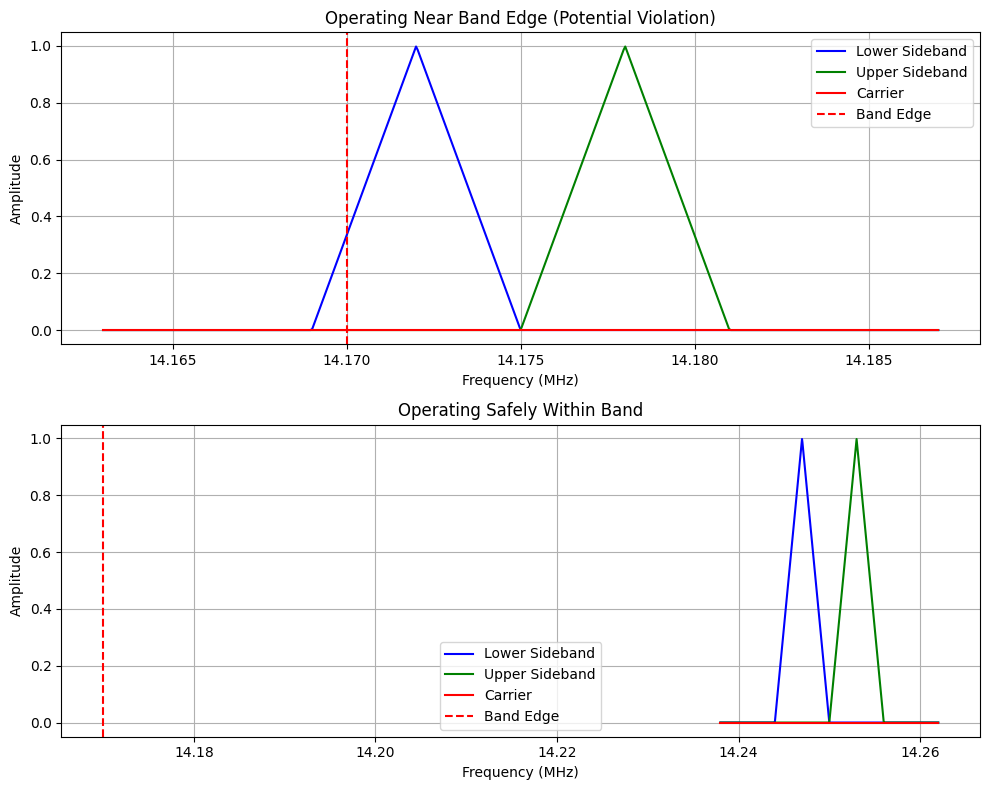
\includegraphics[width=0.8\textwidth]{tech/images/sideband_edge.png}
    \caption{Illustration of Amplitude Modulated (AM) Signal Sidebands and Their Relationship to a Band Edge. The plot depicts two scenarios: (top) a signal operating dangerously close to the lower band edge, with its lower sideband extending beyond the permitted limit; and (bottom) a signal operating safely within the band, with both sidebands contained within the allocated frequencies.}
    \label{fig:sidebands}
    % Prompt: Illustration of modulation sidebands extending beyond the band edge, showing why operating at the edge is discouraged.
    % Software: Matplotlib
\end{figure}


\subsubsection*{Questions}
\begin{tcolorbox}[colback=gray!10!white,colframe=black!75!black,title={T1B01}]
    Which of the following frequency ranges are available for phone operation by Technician licensees?
    \begin{enumerate}[label=\Alph*),noitemsep]
        \item 28.050 MHz to 28.150 MHz
        \item 28.100 MHz to 28.300 MHz
        \item \textbf{28.300 MHz to 28.500 MHz}
        \item 28.500 MHz to 28.600 MHz
    \end{enumerate}
\end{tcolorbox}
Technician licensees have phone privileges on the 10-meter band from 28.300 to 28.500 MHz. The other options fall outside this range.

\begin{tcolorbox}[colback=gray!10!white,colframe=black!75!black,title={T1B02}]
    Which amateurs may contact the International Space Station (ISS) on VHF bands?
    \begin{enumerate}[label=\Alph*),noitemsep]
        \item Any amateur holding a General class or higher license
        \item \textbf{Any amateur holding a Technician class or higher license}
        \item Any amateur holding a General class or higher license who has applied for and received approval from NASA
        \item Any amateur holding a Technician class or higher license who has applied for and received approval from NASA
    \end{enumerate}
\end{tcolorbox}
Any amateur with a Technician class license or higher can contact the ISS on VHF bands. No special approval from NASA is required.

\begin{tcolorbox}[colback=gray!10!white,colframe=black!75!black,title={T1B03}]
    Which frequency is in the 6 meter amateur band?
    \begin{enumerate}[label=\Alph*),noitemsep]
        \item 49.00 MHz
        \item \textbf{52.525 MHz}
        \item 28.50 MHz
        \item 222.15 MHz
    \end{enumerate}
\end{tcolorbox}
The 6-meter band spans 50–54 MHz, so 52.525 MHz falls within this range. The other options are either too low or too high. Another way to remember this is that the product of the frequency (in MHz) and wavelength (in meters) is about 300. So we should be looking for a frequency that is close to 300/6 = 50 MHz. This would eliminate 28.50 MHz and 222.15 MHz. 49.00 MHz is not in the 6-meter band by definition.

\begin{tcolorbox}[colback=gray!10!white,colframe=black!75!black,title={T1B04}]
    Which amateur band includes 146.52 MHz?
    \begin{enumerate}[label=\Alph*),noitemsep]
        \item 6 meters
        \item 20 meters
        \item 70 centimeters
        \item \textbf{2 meters}
    \end{enumerate}
\end{tcolorbox}
146.52 MHz is the national calling frequency for the 2-meter band (144–148 MHz). The other bands don’t include this frequency. We can again use the 300/wavelength rule to infer that 146.52 MHz is in the 2-meter band.

\begin{tcolorbox}[colback=gray!10!white,colframe=black!75!black,title={T1B05}]
    How may amateurs use the 219 to 220 MHz segment of 1.25 meter band?
    \begin{enumerate}[label=\Alph*),noitemsep]
        \item Spread spectrum only
        \item Fast-scan television only
        \item Emergency traffic only
        \item \textbf{Fixed digital message forwarding systems only}
    \end{enumerate}
\end{tcolorbox}
There is no good reason but just because FCC said so.
The 219–220 MHz segment is reserved for fixed digital message forwarding systems. Other modes are not permitted in this segment. (This is a good excuse to get a General license!)

\begin{tcolorbox}[colback=gray!10!white,colframe=black!75!black,title={T1B06}]
    On which HF bands does a Technician class operator have phone privileges?
    \begin{enumerate}[label=\Alph*),noitemsep]
        \item None
        \item \textbf{10 meter band only}
        \item 80 meter, 40 meter, 15 meter, and 10 meter bands
        \item 30 meter band only
    \end{enumerate}
\end{tcolorbox}
Technician licensees have phone privileges only on the 10-meter band (28.300–28.500 MHz). The other bands are either not available or restricted to CW or digital modes.

\begin{tcolorbox}[colback=gray!10!white,colframe=black!75!black,title={T1B07}]
    Which of the following VHF/UHF band segments are limited to CW only?
    \begin{enumerate}[label=\Alph*),noitemsep]
        \item \textbf{50.0 MHz to 50.1 MHz and 144.0 MHz to 144.1 MHz}
        \item 219 MHz to 220 MHz and 420.0 MHz to 420.1 MHz
        \item 902.0 MHz to 902.1 MHz
        \item All these choices are correct
    \end{enumerate}
\end{tcolorbox}
The 50.0–50.1 MHz and 144.0–144.1 MHz segments are reserved for CW only. The other segments allow different modes.

\begin{tcolorbox}[colback=gray!10!white,colframe=black!75!black,title={T1B08}]
    How are US amateurs restricted in segments of bands where the Amateur Radio Service is secondary?
    \begin{enumerate}[label=\Alph*),noitemsep]
        \item \textbf{U.S. amateurs may find non-amateur stations in those segments, and must avoid interfering with them}
        \item U.S. amateurs must give foreign amateur stations priority in those segments
        \item International communications are not permitted in those segments
        \item Digital transmissions are not permitted in those segments
    \end{enumerate}
\end{tcolorbox}
In secondary segments, amateurs must avoid interfering with primary users, which may include non-amateur stations. There’s no requirement to prioritize foreign amateur stations or restrict international communications.

\begin{tcolorbox}[colback=gray!10!white,colframe=black!75!black,title={T1B09}]
    Why should you not set your transmit frequency to be exactly at the edge of an amateur band or sub-band?
    \begin{enumerate}[label=\Alph*),noitemsep]
        \item To allow for calibration error in the transmitter frequency display
        \item So that modulation sidebands do not extend beyond the band edge
        \item To allow for transmitter frequency drift
        \item \textbf{All these choices are correct}
    \end{enumerate}
\end{tcolorbox}
All of these reasons are valid. Operating near the band edge risks interference due to calibration errors, sideband spillover, and frequency drift.

\begin{tcolorbox}[colback=gray!10!white,colframe=black!75!black,title={T1B10}]
    Where may SSB phone be used in amateur bands above 50 MHz?
    \begin{enumerate}[label=\Alph*),noitemsep]
        \item Only in sub-bands allocated to General class or higher licensees
        \item Only on repeaters
        \item \textbf{In at least some segment of all these bands}
        \item On any band if the power is limited to 25 watts
    \end{enumerate}
\end{tcolorbox}
We haven't talked about SSB yet, for now just remember that SSB phone is permitted in at least some segment of all amateur bands above 50 MHz. It’s not limited to repeaters or specific license classes.

\begin{tcolorbox}[colback=gray!10!white,colframe=black!75!black,title={T1B11}]
    What is the maximum peak envelope power output for Technician class operators in their HF band segments?
    \begin{enumerate}[label=\Alph*),noitemsep]
        \item \textbf{200 watts}
        \item 100 watts
        \item 50 watts
        \item 10 watts
    \end{enumerate}
\end{tcolorbox}
Technician licensees are limited to 200 watts PEP on their HF band segments. This ensures they can operate effectively without causing excessive interference.

We will discuss what PEP is in more detail in later chapters.

\begin{tcolorbox}[colback=gray!10!white,colframe=black!75!black,title={T1B12}]
    Except for some specific restrictions, what is the maximum peak envelope power output for Technician class operators using frequencies above 30 MHz?
    \begin{enumerate}[label=\Alph*),noitemsep]
        \item 50 watts
        \item 100 watts
        \item 500 watts
        \item \textbf{1500 watts}
    \end{enumerate}
\end{tcolorbox}
Technician licensees can operate at up to 1500 watts PEP on frequencies above 30 MHz, unless specific restrictions apply (e.g., in certain sub-bands or near band edges).

For maximum power restrictions, see Table~\ref{tab:license_privileges}. Just remember that all licensees can use up to 1500W PEP for any band, except for Technician licensees who are limited to 200W PEP on their HF band segments.
% \section{Getting Your License}
% \subsection{Obtaining and Renewing}
\label{subsec:obtain-renew}

So, you've decided to dive into the world of amateur radio! Congratulations! But before you can start chatting with fellow hams across the globe, you'll need to get your hands on a license. Let's break down the process, step by step.

\subsubsection{License Exam}
First things first, you need to pass an exam. You can take the exam in-person or online. 
I can share my experience that the online exam is much easier to take as long as you are comfortable with video conferencing.  

The first step is to register at the FCC Commission Registration System\footnote{https://apps.fcc.gov/cores/}. This is to obtain your FCC FRN\footnote{An FRN is a Federal Communications Commission Registration Number} number. 

Then you need to register for an exam session. The most user friendly portal to find an exam session would be on HamStudy\footnote{https://hamstudy.org/sessions/remote}. You can find the exam session that is the most convenient for you. You'll need to use your FRN number. The fee for the exam is typically \$15, you have to pay it online before the exam. 

Before the exam, the exam team will send you an email with the exam instructions with a Zoom link. The email has the tendency to go to your spam folder, so make sure to check it. 

During the exam, the examiners will ask you to show both your physical and computer environments. So I'd suggest you to be alone in a simple room with a clean desk and a closed door. Remove all smart devices from your desk and from your body. That means you should put away your smart watch, smart glasses, smart phone, smart shoes, and smart anything. This doesn't mean your dumb brother can stay in the room with you. You should also close all programs on your computer except for a web browser. The examiners would allow you to use a physical calculator or the calculator app on your computer for the exam but you should be able to do the technician exam without it. 

You have to show a photo ID to the examiners before the exam. 

The exam is a multiple choice exam. You will have 90 minutes to complete the exam. For Technician and General class, you need to get 26  out of 35 questions correct to pass. For Extra class, you need to get 37 out of 50 questions correct to pass. 

The online exam is exactly the same format as the practice exams on the HamStudy website. You should definitely get their mobile app to practice the exam questions while you are waiting in a cashier line. 

The examiners, from all 3 exams I took, were the most friendly and helpful you can imagine. But they are also very strict. There will be at least 3 examiners there  overseeing you taking the exam. They will be watching your every move. I had the pleasure to have 14(!) examiners watching me as the lone examinee taking the General exam, and 9 for the Extra exam, no pressure at all. 


\subsubsection{License Grant}
Once you've aced tje, the FCC (Federal Communications Commission) will issue you an operator/primary station license grant, and a call sign. But you need to pay a \$35 fee to the FCC to get your license. 

Now, here's the kicker: you can only hold one of these at a time. That's right, no hoarding licenses for different bands or locations. Just one per person, as per FCC rules.


\subsubsection{FCC ULS Database}
Once the FCC grants your license, it will appear in the FCC ULS (Universal Licensing System) database. This is your golden ticket. If your license is in the ULS, you're good to go. No need to wait for a physical copy in the mail or an email notification. The ULS is the ultimate authority on your licensing status.

\subsubsection*{License Term and Grace Period}
Your shiny new license is valid for ten years. Yes, a whole decade of radio fun! But what happens if you forget to renew it? Don't worry, the FCC has a grace period of two years. During this time, you can still renew your license without having to retake the exam. However, and this is important, you cannot transmit during the grace period. You must wait until your license is officially renewed.

\subsubsection*{Transmission Authorization}
Once your license appears in the ULS database, you're officially authorized to transmit. No need to wait for a physical copy or any other confirmation. The ULS is your go-to source for all things licensing.


\begin{table}[h]
    \centering
    \begin{tabular}{|l|l|}
        \hline
        \textbf{Key Point} & \textbf{Details} \\ \hline
        License Grant & One per person, issued by the FCC \\ \hline
        FCC ULS Database & Official record of license status \\ \hline
        License Term & 10 years \\ \hline
        Grace Period & 2 years, no transmission allowed \\ \hline
        Transmission Authorization & Upon ULS database entry \\ \hline
    \end{tabular}
    \caption{Summary of License Obtaining and Renewing}
    \label{tab:license-summary}
\end{table}

\subsubsection*{Questions}

\begin{tcolorbox}[colback=gray!10!white,colframe=black!75!black,title={T1A04}]
    How many operator/primary station license grants may be held by any one person?
    \begin{enumerate}[label=\Alph*),noitemsep]
        \item \textbf{One}
        \item No more than two
        \item One for each band on which the person plans to operate
        \item One for each permanent station location from which the person plans to operate
    \end{enumerate}
\end{tcolorbox}
The FCC allows only one operator/primary station license grant per person. This ensures that each licensee is responsible for their own station and operations.

\begin{tcolorbox}[colback=gray!10!white,colframe=black!75!black,title={T1A05}]
    What proves that the FCC has issued an operator/primary license grant?
    \begin{enumerate}[label=\Alph*),noitemsep]
        \item A printed copy of the certificate of successful completion of examination
        \item An email notification from the NCVEC granting the license
        \item \textbf{The license appears in the FCC ULS database}
        \item All these choices are correct
    \end{enumerate}
\end{tcolorbox}
The FCC ULS database is the official record of your license status. If your license is listed there, it's official.

\begin{tcolorbox}[colback=gray!10!white,colframe=black!75!black,title={T1C08}]
    What is the normal term for an FCC-issued amateur radio license?
    \begin{enumerate}[label=\Alph*),noitemsep]
        \item Five years
        \item Life
        \item \textbf{Ten years}
        \item Eight years
    \end{enumerate}
\end{tcolorbox}
An amateur radio license is valid for ten years. After that, you'll need to renew it to continue operating.

\begin{tcolorbox}[colback=gray!10!white,colframe=black!75!black,title={T1C09}]
    What is the grace period for renewal if an amateur license expires?
    \begin{enumerate}[label=\Alph*),noitemsep]
        \item \textbf{Two years}
        \item Three years
        \item Five years
        \item Ten years
    \end{enumerate}
\end{tcolorbox}
The grace period for renewing an expired license is two years. During this time, you can renew without retaking the exam, but you cannot transmit.

\begin{tcolorbox}[colback=gray!10!white,colframe=black!75!black,title={T1C10}]
    How soon after passing the examination for your first amateur radio license may you transmit on the amateur radio bands?
    \begin{enumerate}[label=\Alph*),noitemsep]
        \item Immediately on receiving your Certificate of Successful Completion of Examination (CSCE)
        \item As soon as your operator/station license grant appears on the ARRL website
        \item \textbf{As soon as your operator/station license grant appears in the FCC’s license database}
        \item As soon as you receive your license in the mail from the FCC
    \end{enumerate}
\end{tcolorbox}
You can start transmitting as soon as your license appears in the FCC ULS database. No need to wait for physical copies or other confirmations.

\begin{tcolorbox}[colback=gray!10!white,colframe=black!75!black,title={T1C11}]
    If your license has expired and is still within the allowable grace period, may you continue to transmit on the amateur radio bands?
    \begin{enumerate}[label=\Alph*),noitemsep]
        \item Yes, for up to two years
        \item Yes, as soon as you apply for renewal
        \item Yes, for up to one year
        \item \textbf{No, you must wait until the license has been renewed}
    \end{enumerate}
\end{tcolorbox}
Even if your license is within the grace period, you cannot transmit until it has been officially renewed. This ensures that all operators are properly licensed and compliant with FCC regulations.

% \subsection{Call Signs}
\label{subsec:call-signs}

In the world of amateur radio, call signs are like your personal identifier—your radio name, if you will. They are unique to each operator and are used to identify who is transmitting. Let’s dive into the rules and formats for these call signs, and maybe have a little fun along the way.

\subsubsection*{Vanity Call Sign Rules}
Ever wanted to pick your own call sign? Well, under the vanity call sign rules, you can! Any licensed amateur, regardless of their license class, can select a desired call sign. That’s right, whether you’re a Technician, General, or Extra class operator, you can choose a call sign that resonates with you. This is a great way to personalize your presence on the airwaves. Just remember, the call sign you choose must still follow the FCC’s format rules.

\subsubsection*{Call Sign Formats}
Now, let's talk about the structure of these call signs. In the United States, amateur radio call signs follow specific format rules based on the license class and region. Here's how they break down:

\begin{itemize}
    \item \textbf{Prefix}: 1 or 2 letters, starting with K, N, or W (and some special cases with AA-AL, KA-KZ, NA-NZ, WA-WZ)
    \item \textbf{Region Number}: A single digit (0-9) indicating the geographic region\footnote{https://www.radioqth.net/vanity/SeqCallSystem}
    \item \textbf{Suffix}: 1 to 3 letters
\end{itemize}

For Technician class operators, the call sign typically follows formats like:
\begin{itemize}
    \item 2x3 format: Two-letter prefix, one number, three-letter suffix (e.g., \texttt{KF1XXX})
    \item 1x3 format: One-letter prefix, one number, three-letter suffix (e.g., \texttt{K1XXX})
\end{itemize}

The length of the suffix can indicate license class:
\begin{itemize}
    \item 2-letter suffix (1x2): Usually reserved for Extra class
    \item 3-letter suffix (1x3 or 2x3): Common for Technician and General class
\end{itemize}

\begin{figure}[h]
    \centering
    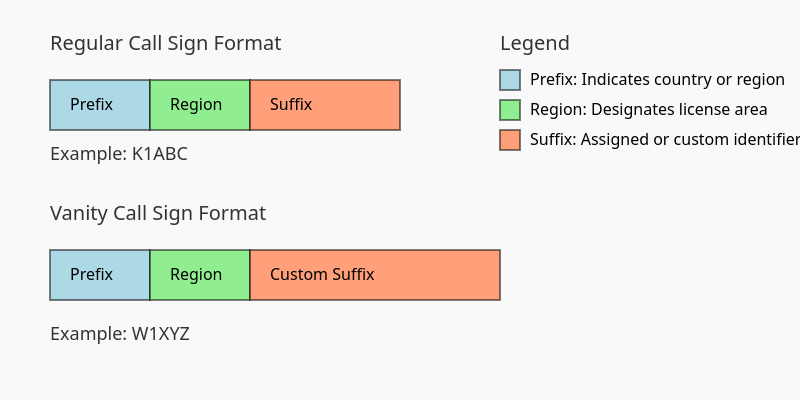
\includegraphics[width=0.8\textwidth]{tech/images/call-sign-structure.png}
    \caption{Structure of an Amateur Radio Call Sign}
    \label{fig:call-sign-structure}
    % Diagram showing the structure of a typical amateur radio call sign.
\end{figure}

\begin{table}[h]
    \centering
    \begin{tabular}{|l|l|l|}
        \hline
        \textbf{Format} & \textbf{Example} & \textbf{Typical Class} \\
        \hline
        1x2 & W1XX & Extra \\
        1x3 & K1XXX & General/Tech \\
        2x3 & KF1XXX & Tech/General \\
        \hline
    \end{tabular}
    \caption{Common Call Sign Formats}
    \label{tab:call-sign-formats}
\end{table}

\subsubsection*{Questions}

\begin{tcolorbox}[colback=gray!10!white,colframe=black!75!black,title={T1C02}]
    Who may select a desired call sign under the vanity call sign rules?
    \begin{enumerate}[label=\Alph*),noitemsep]
        \item Only a licensed amateur with a General or Amateur Extra Class license
        \item Only a licensed amateur with an Amateur Extra Class license
        \item Only a licensed amateur who has been licensed continuously for more than 10 years
        \item \textbf{Any licensed amateur}
    \end{enumerate}
\end{tcolorbox}

Under the vanity call sign rules, any licensed amateur, regardless of their license class, can select a desired call sign. This means even a Technician class operator can choose a call sign that suits them. However, only an Amateur Extra Class operator can select a call sign that is 1x2 or 2x1.

\begin{tcolorbox}[colback=gray!10!white,colframe=black!75!black,title={T1C05}]
    Which of the following is a valid Technician class call sign format?
    \begin{enumerate}[label=\Alph*),noitemsep]
        \item \textbf{KF1XXX}
        \item KA1X
        \item W1XX
        \item All these choices are correct
    \end{enumerate}
\end{tcolorbox}

The correct format for a Technician class call sign is \texttt{KF1XXX}. This format includes a prefix (\texttt{KF}), a number (\texttt{1}), and a suffix (\texttt{XXX}). The other options either do not follow the correct format or are incomplete. Therefore, the correct answer is \textbf{A}.

% \subsection{License Maintenance, Contact Information}
\label{subsec:maint-contact}

Maintaining accurate contact information with the FCC is not just a bureaucratic formality—it’s a critical part of being a responsible amateur radio operator. Imagine the FCC trying to reach you about an important update or issue, only to find that your email address is outdated. Spoiler alert: it doesn’t end well. Let’s dive into why this matters and what could happen if you drop the ball.

\subsubsection*{Why Accurate Contact Information Matters}
The FCC requires you to provide and maintain a correct email address. Why? Because email is their primary method of communication with licensees. If they can’t reach you, they can’t notify you about important updates, rule changes, or even issues with your station. And trust me, you don’t want to be in the dark about those things.

\subsubsection*{Consequences of Failing to Maintain Contact Information}
If the FCC is unable to reach you by email, they have the authority to take action. This could include revoking your station license or suspending your operator license. Yes, you read that right—your license could be on the line. This isn’t just a slap on the wrist; it’s a serious consequence for what might seem like a minor oversight.


\begin{table}[h!]
    \centering
    \begin{tabular}{|l|l|}
        \hline
        \textbf{Requirement} & \textbf{Consequence} \\
        \hline
        Provide a correct email address & Revocation of station license or suspension of operator license \\
        \hline
        Update contact information promptly & Avoid fines and license issues \\
        \hline
    \end{tabular}
    \caption{Summary of License Maintenance and Contact Information Requirements}
    \label{tab:license-maintenance-summary}
\end{table}

\subsubsection{Questions}

\begin{tcolorbox}[colback=gray!10!white,colframe=black!75!black,title={T1C04}]
What may happen if the FCC is unable to reach you by email?
\begin{enumerate}[label=\Alph*),noitemsep]
    \item Fine and suspension of operator license
    \item \textbf{Revocation of the station license or suspension of the operator license}
    \item Revocation of access to the license record in the FCC system
    \item Nothing; there is no such requirement
\end{enumerate}
\end{tcolorbox}

If the FCC can’t reach you by email, they have the authority to revoke your station license or suspend your operator license. This is because email is their primary method of communication, and they need to be able to contact you for important updates or issues. Options A and C are incorrect because the FCC’s primary concern is communication, not fines or access to records. Option D is incorrect because there is indeed a requirement to maintain a correct email address.

\begin{tcolorbox}[colback=gray!10!white,colframe=black!75!black,title={T1C07}]
Which of the following can result in revocation of the station license or suspension of the operator license?
\begin{enumerate}[label=\Alph*),noitemsep]
    \item Failure to inform the FCC of any changes in the amateur station following performance of an RF safety environmental evaluation
    \item \textbf{Failure to provide and maintain a correct email address with the FCC}
    \item Failure to obtain FCC type acceptance prior to using a home-built transmitter
    \item Failure to have a copy of your license available at your station
\end{enumerate}
\end{tcolorbox}

Failure to provide and maintain a correct email address with the FCC can result in revocation of your station license or suspension of your operator license. This is because the FCC relies on email to communicate with licensees. Option A is incorrect because while RF safety evaluations are important, they don’t directly relate to contact information. Option C is incorrect because type acceptance is about equipment, not contact information. Option D is incorrect because while having a copy of your license at your station is a good practice, it’s not directly related to contact information.

% \subsection{Operating Locations}
\label{subsec:operating-location}

When it comes to operating your FCC-licensed amateur station, the rules about where you can transmit are pretty straightforward, but they do have some interesting nuances. Let's dive into the specifics, especially when it comes to operating from international waters.

First off, you might be wondering, "Can I just set up my station anywhere in the world and start transmitting?" Well, not quite. The FCC has some clear guidelines on this. According to FCC regulations, an FCC-licensed amateur station can transmit from any vessel or craft located in international waters, provided that the vessel or craft is documented or registered in the United States. This means that if you're on a U.S.-registered boat in the middle of the ocean, you're good to go!

But what about on land? The rules are a bit different there. You can't just set up shop in any country and start transmitting. The FCC doesn't have jurisdiction outside the United States, so you need to be mindful of the local laws and regulations of the country you're in. However, if you're in a country that belongs to the International Telecommunication Union (ITU), you might have some leeway, but it's always best to check with the local authorities.

Now, let's talk about international waters. These are areas of the ocean that are not under the jurisdiction of any single country. If you're on a U.S.-registered vessel in these waters, you're essentially operating under U.S. jurisdiction, which means you can transmit as long as you follow FCC rules. This is a great option for those who love to combine their passion for amateur radio with a bit of maritime adventure.

% To help visualize this, take a look at Figure~\ref{fig:operating-locations-map}, which shows the permissible operating locations for FCC-licensed amateur stations. The map highlights the areas where you can legally operate your station, including international waters.

% \begin{figure}[h]
%     \centering
%     % \includegraphics[width=0.8\textwidth]{operating-locations-map.png}
%     \caption{Permissible Operating Locations for FCC-Licensed Amateur Stations}
%     \label{fig:operating-locations-map}
%     % Prompt: Map showing permissible operating locations for FCC-licensed amateur stations. The map should highlight international waters and areas under U.S. jurisdiction.
% \end{figure}

For a quick summary of the rules, refer to Table~\ref{tab:operating-location-summary}. This table breaks down the key points about where you can and cannot operate your amateur station.

\begin{table}[h]
    \centering
    \begin{tabular}{|l|l|}
        \hline
        \textbf{Location} & \textbf{Permission} \\
        \hline
        U.S. Territory & Allowed \\
        International Waters (U.S.-registered vessel) & Allowed \\
        ITU Member Countries & Check Local Laws \\
        Non-ITU Member Countries & Generally Not Allowed \\
        \hline
    \end{tabular}
    \caption{Summary of Operating Location Rules}
    \label{tab:operating-location-summary}
\end{table}

\subsubsection*{Questions}

\begin{tcolorbox}[colback=gray!10!white,colframe=black!75!black,title={T1C06}]
    From which of the following locations may an FCC-licensed amateur station transmit?
    \begin{enumerate}[label=\Alph*),noitemsep]
        \item From within any country that belongs to the International Telecommunication Union
        \item From within any country that is a member of the United Nations
        \item From anywhere within International Telecommunication Union (ITU) Regions 2 and 3
        \item \textbf{From any vessel or craft located in international waters and documented or registered in the United States}
    \end{enumerate}
\end{tcolorbox}

The correct answer is \textbf{D}. According to FCC regulations, an FCC-licensed amateur station may transmit from any vessel or craft located in international waters, provided that the vessel or craft is documented or registered in the United States. This is a specific provision that allows amateur radio operators to operate in international waters under U.S. jurisdiction. Options A, B, and C are incorrect because they do not align with the FCC's specific rules regarding operating locations. While ITU membership or UN membership might imply certain international agreements, they do not override the FCC's jurisdiction requirements for amateur radio operations.

% \part{FCC Rules and Station Operation}
% \chapter{FCC Rules and Regulations}
% \section{Regulatory Framework}
% \subsection{Definitions, Basis, and Purpose}
\label{subsec:reg-basis}

Welcome to the section where we dive into the nitty-gritty of radio regulations! Don't worry, we'll keep it light and conversational, even though we're dealing with some serious topics. By now, you've probably got a good grasp of the basics, so let's build on that foundation.

In this subsection, we'll explore the definitions, basis, and purpose behind the regulations that govern radio technology. These rules aren't just arbitrary; they're designed to ensure that everyone can enjoy clear, interference-free communication. Think of it as the traffic laws of the airwaves—without them, it would be chaos!

\subsubsection*{Why Do We Need These Regulations?}

You might be wondering, "Why do we need all these rules?" Well, imagine a world where everyone could transmit on any frequency they wanted, at any power level. It would be like trying to have a conversation in a crowded room where everyone is shouting at the top of their lungs. Not very effective, right? The regulations help to keep things orderly, so that everyone can communicate without stepping on each other's toes.

\subsubsection*{The Basis of Radio Regulations}

The basis for these regulations comes from a combination of physics, engineering, and good old-fashioned common sense. For example, the Federal Communications Commission (FCC) in the United States has a set of rules known as Part 97, which governs amateur radio operations. These rules are based on the idea that amateur radio operators should have the freedom to experiment and communicate, but not at the expense of others.

\subsubsection*{The Purpose Behind the Rules}

The purpose of these regulations is to promote the efficient use of the radio spectrum, ensure safety, and encourage innovation. By setting clear guidelines, the regulations help to prevent interference, protect public safety, and foster a community of knowledgeable and responsible radio operators.

So, as we move forward, keep in mind that these regulations aren't just red tape—they're the backbone of a system that allows us to communicate effectively and safely. And who knows, maybe you'll even find some humor in the process!

\subsubsection*{What's Next?}

Now that we've laid the groundwork, we'll move on to more specific topics, like frequency allocation, power limits, and licensing requirements. But don't worry, we'll keep the tone light and the explanations clear. After all, radio technology should be fun, not frustrating!


% \section{Authorized vs. Prohibited Communications}
% \subsection{International Communications, Third-Party Traffic}
\label{subsec:intl-third-party}

In the world of amateur radio, communication isn't just about chatting with your neighbor down the street. Sometimes, it's about connecting with someone halfway across the globe. But before you start dreaming of chatting with a ham operator in Antarctica, let's talk about the rules—specifically, international communications and third-party traffic.

\subsubsection*{Third-Party Communications}

Third-party communications in amateur radio are like being the middleman in a conversation. Imagine you're the control operator of a station, and your friend, who isn't licensed, wants to send a message to another amateur station. You, as the control operator, are responsible for ensuring that the message is transmitted correctly and that all regulations are followed. This is what we call third-party communications.

The key here is that the control operator must always be in control of the station. The third party (your unlicensed friend) can speak, but you're the one who ensures everything is done by the book. There are also restrictions, especially when it comes to international communications. For example, the foreign station must be in a country with which the U.S. has a third-party agreement. This ensures that both sides are playing by the same rules.

\subsubsection*{International Communications}

When it comes to international communications, the FCC has some specific guidelines. Amateur radio stations are allowed to make communications that are incidental to the purposes of the Amateur Radio Service. This means you can chat about personal stuff, as long as it's not business-related. So, no trying to sell your homemade antennas to someone in France!

But here's the catch: if you're allowing a non-licensed person to speak to a foreign station, there are additional restrictions. The foreign station must be in a country with which the U.S. has a third-party agreement. This is to ensure that the communication is legal on both ends. And, of course, the licensed control operator must do the station identification. You can't just let your friend take over the mic without proper oversight.



\subsubsection*{What Counts as Personal Remarks}
When we talk about "personal remarks" in amateur radio, we're referring to casual, non-business conversations about your daily life, hobbies, experiences, and other personal topics. These are the friendly chats that make amateur radio such an engaging hobby.


Personal remarks typically include:
\begin{itemize}[noitemsep]
    \item Discussion about your radio equipment and setup
    \item Weather conditions in your area
    \item Family news and activities
    \item Personal experiences and stories
    \item Hobbies and interests
    \item Technical discussions and experimentation
    \item Health and welfare messages during emergencies
\end{itemize}

\subsubsection*{What's Not Allowed}
To maintain the non-commercial nature of amateur radio, these topics are prohibited:
\begin{itemize}[noitemsep]
    \item Business transactions or advertisements
    \item Promoting products or services
    \item Professional activities for compensation
    \item Political lobbying or fundraising
    \item Obscene or indecent language
\end{itemize}

\subsubsection{Questions}

\begin{tcolorbox}[colback=gray!10!white,colframe=black!75!black,title={T1C03}]
    What types of international communications are an FCC-licensed amateur radio station permitted to make?
    \begin{enumerate}[label=\Alph*),noitemsep]
        \item \textbf{Communications incidental to the purposes of the Amateur Radio Service and remarks of a personal character}
        \item Communications incidental to conducting business or remarks of a personal nature
        \item Only communications incidental to contest exchanges; all other communications are prohibited
        \item Any communications that would be permitted by an international broadcast station
    \end{enumerate}
\end{tcolorbox}

According to FCC regulations, amateur radio stations are allowed to make communications that are incidental to the purposes of the Amateur Radio Service, which includes personal remarks. Business-related communications are strictly prohibited.

\begin{tcolorbox}[colback=gray!10!white,colframe=black!75!black,title={T1F07}]
    Which of the following restrictions apply when a non-licensed person is allowed to speak to a foreign station using a station under the control of a licensed amateur operator?
    \begin{enumerate}[label=\Alph*),noitemsep]
        \item The person must be a U.S. citizen
        \item \textbf{The foreign station must be in a country with which the U.S. has a third party agreement}
        \item The licensed control operator must do the station identification
        \item All these choices are correct
    \end{enumerate}
\end{tcolorbox}

The foreign station must be in a country with which the U.S. has a third-party agreement. This ensures that the communication is legal on both ends. The control operator must also handle the station identification, but the person speaking does not need to be a U.S. citizen.

\begin{tcolorbox}[colback=gray!10!white,colframe=black!75!black,title={T1F08}]
    What is the definition of third party communications?
    \begin{enumerate}[label=\Alph*),noitemsep]
        \item \textbf{A message from a control operator to another amateur station control operator on behalf of another person}
        \item Amateur radio communications where three stations are in communications with one another
        \item Operation when the transmitting equipment is licensed to a person other than the control operator
        \item Temporary authorization for an unlicensed person to transmit on the amateur bands for technical experiments
    \end{enumerate}
\end{tcolorbox}

Third-party communications involve a control operator transmitting a message on behalf of another person. This is a common scenario in amateur radio, especially when the third party is not licensed.

% \subsection{Prohibited Content}
\label{subsec:prohibited-content}

In the world of amateur radio, not everything goes. There are specific rules and regulations that govern what you can and cannot transmit. Let's dive into some of the key prohibitions, starting with broadcasting and indecent language.

\subsubsection*{Broadcasting in Amateur Radio}
Broadcasting, in the context of amateur radio, refers to transmissions intended for reception by the general public. This is generally prohibited because amateur radio is meant for two-way communication, not for sending out content to a wide audience. Think of it like this: you're at a party, and instead of having a conversation, you start giving a speech to everyone in the room. That's not what amateur radio is for!

The FCC defines broadcasting as "transmissions intended for reception by the general public" (FCC Part 97.3(a)(10)). This means that if you're sending out a message that isn't directed at a specific individual or group, you're likely violating the rules.

\subsubsection*{Prohibited Language}
Another big no-no in amateur radio is the use of indecent or obscene language. The FCC has clear rules about this: any such language is prohibited. This means that you need to keep your transmissions clean and professional. Remember, amateur radio is a public service, and your transmissions could be heard by anyone, including children.

\subsubsection*{Summary of Prohibited Content}
To help you keep track of what's allowed and what's not, here's a quick summary of the types of prohibited content in amateur radio communications:

\begin{table}[h]
\centering
\caption{Prohibited Content in Amateur Radio}
\label{tab:prohibited-content}
\begin{tabular}{|l|l|}
\hline
\textbf{Type of Content} & \textbf{Description} \\
\hline
Broadcasting & Transmissions intended for the general public \\
Indecent/Obscene Language & Any language considered indecent or obscene \\
\hline
\end{tabular}
\end{table}

% \subsubsection*{Illustration: Broadcasting vs. Two-Way Communication}
% To better understand the difference between broadcasting and two-way communication, take a look at Figure~\ref{fig:broadcast-vs-two-way}. The illustration shows how broadcasting sends a message out to a wide audience, while two-way communication is a back-and-forth exchange between specific individuals.

% \begin{figure}[h]
% \centering
% % \includegraphics[width=0.8\textwidth]{broadcast-vs-two-way}
% \caption{Broadcasting vs. Two-Way Communication in Amateur Radio}
% \label{fig:broadcast-vs-two-way}
% \end{figure}

\subsubsection{Questions}

\begin{tcolorbox}[colback=gray!10!white,colframe=black!75!black,title={T1D02}]
Under which of the following circumstances are one-way transmissions by an amateur station prohibited?
\begin{enumerate}[label=\Alph*),noitemsep]
    \item In all circumstances
    \item \textbf{Broadcasting}
    \item International Morse Code Practice
    \item Telecommand or transmissions of telemetry
\end{enumerate}
\end{tcolorbox}

Broadcasting is the correct answer because one-way transmissions intended for the general public are prohibited in amateur radio. The other options, such as International Morse Code Practice and telecommand, are allowed under specific circumstances.

\begin{tcolorbox}[colback=gray!10!white,colframe=black!75!black,title={T1D06}]
What, if any, are the restrictions concerning transmission of language that may be considered indecent or obscene?
\begin{enumerate}[label=\Alph*),noitemsep]
    \item The FCC maintains a list of words that are not permitted to be used on amateur frequencies
    \item \textbf{Any such language is prohibited}
    \item The ITU maintains a list of words that are not permitted to be used on amateur frequencies
    \item There is no such prohibition
\end{enumerate}
\end{tcolorbox}

Any indecent or obscene language is prohibited in amateur radio transmissions. The FCC does not maintain a specific list of prohibited words, but the general rule is clear: keep it clean.

\begin{tcolorbox}[colback=gray!10!white,colframe=black!75!black,title={T1D10}]
How does the FCC define broadcasting for the Amateur Radio Service?
\begin{enumerate}[label=\Alph*),noitemsep]
    \item Two-way transmissions by amateur stations
    \item Any transmission made by the licensed station
    \item Transmission of messages directed only to amateur operators
    \item \textbf{Transmissions intended for reception by the general public}
\end{enumerate}
\end{tcolorbox}

The FCC defines broadcasting as "transmissions intended for reception by the general public." This is the key distinction between broadcasting and other types of transmissions in amateur radio.

% \subsection{Business Communications, Broadcasting, Music}
\label{subsec:biz-broadcast-music}

Amateur radio operators often wonder about the boundaries of what they can and cannot do with their stations, especially when it comes to business communications and broadcasting music. Let's dive into the specifics of these rules, so you can stay on the right side of the regulations while still having fun with your radio.

\subsubsection*{Music Transmission in Amateur Radio}
One of the most common questions is: "Can I play music over my amateur radio station?" The answer is yes, but only under very specific conditions. According to FCC regulations, music can be transmitted using a phone emission if it is \textit{incidental to an authorized retransmission of manned spacecraft communications}. This means that if you're retransmitting communications from a manned spacecraft (like the International Space Station), and there happens to be music in the background, you're in the clear. However, playing your favorite tunes just for fun? That's a no-go.

% \begin{figure}[h]
%     \centering
%     % \includegraphics[width=0.8\textwidth]{figures/music-transmission.png}
%     \caption{Permitted Scenarios for Music Transmission in Amateur Radio}
%     \label{fig:music-transmission}
%     % Diagram showing the scenarios where music transmission is permitted in amateur radio.
%     % The figure should include a flowchart with nodes representing different scenarios, such as "Retransmission of Spacecraft Communications" and "Incidental Music Transmission."
% \end{figure}

\subsubsection*{Business Communications and Equipment Sales}
Now, let's talk about business communications. Amateur radio stations are not meant for commercial use, but there are some exceptions. For example, you can use your station to notify other amateurs about equipment that's available for sale or trade, as long as it's not done on a regular basis. This means you can't turn your amateur radio station into a full-time eBay for radio gear. The key here is that the sale should be occasional and not part of a regular business operation.

\subsubsection{Questions}

\begin{tcolorbox}[colback=gray!10!white,colframe=black!75!black,title={T1D04}]
    Under what conditions is an amateur station authorized to transmit music using a phone emission?
    \begin{enumerate}[label=\Alph*),noitemsep]
        \item \textbf{When incidental to an authorized retransmission of manned spacecraft communications}
        \item When the music produces no spurious emissions
        \item When transmissions are limited to less than three minutes per hour
        \item When the music is transmitted above 1280 MHz
    \end{enumerate}
\end{tcolorbox}

Music can only be transmitted if it is incidental to the retransmission of manned spacecraft communications. This is a very specific scenario, and it's important to remember that playing music for entertainment purposes is not allowed.

\begin{tcolorbox}[colback=gray!10!white,colframe=black!75!black,title={T1D05}]
    When may amateur radio operators use their stations to notify other amateurs of the availability of equipment for sale or trade?
    \begin{enumerate}[label=\Alph*),noitemsep]
        \item Never
        \item When the equipment is not the personal property of either the station licensee, or the control operator, or their close relatives
        \item When no profit is made on the sale
        \item \textbf{When selling amateur radio equipment and not on a regular basis} 
    \end{enumerate}
\end{tcolorbox}

Amateur radio operators can notify others about equipment for sale or trade, but it must not be done on a regular basis. This ensures that the amateur radio service is not used as a commercial platform.



% \subsection{Coded Messages, News Gathering}
\label{subsec:coded-news}

In this section, we'll dive into the fascinating world of coded messages and news gathering in amateur radio. Don't worry, we won't be cracking any secret codes or breaking news stories, but we will explore the rules and conditions under which these activities are permitted. So, grab your decoder rings and let's get started!

\subsubsection*{Coded Messages}
Coded messages in amateur radio are like the secret handshakes of the radio world—they're not for everyone, and there are strict rules about when and how they can be used. According to FCC regulations, transmitting messages encoded to obscure their meaning is generally a big no-no. However, there are a few exceptions to this rule. For example, you can use coded messages when transmitting control commands to space stations or radio control craft. This makes sense, right? You wouldn't want your drone to start doing loop-de-loops because someone accidentally sent it the wrong signal!

\subsubsection*{News Gathering}
Now, let's talk about news gathering. Amateur radio operators are not typically in the business of breaking news, but there are times when they can lend a hand. For instance, if there's an emergency situation where human life or property is at immediate risk, and no other means of communication is available, amateur stations can transmit information in support of broadcasting, program production, or news gathering. This is a great example of how amateur radio can step up in times of crisis.

% \begin{figure}[h]
%     \centering
%     % \includegraphics[width=0.8\textwidth]{figures/coded-news-flow.png}
%     \caption{Conditions for Coded Messages and News Gathering in Amateur Radio}
%     \label{fig:coded-news-flow}
%     % Flowchart showing the conditions under which coded messages and news gathering are permitted in amateur radio. The flowchart should include decision points for coded messages (e.g., "Is the message a control command for a space station or radio control craft?") and news gathering (e.g., "Is there an immediate safety concern?").
% \end{figure}

% \begin{table}[h]
%     \centering
%     \begin{tabular}{|l|l|}
%         \hline
%         \textbf{Activity} & \textbf{Permitted Conditions} \\
%         \hline
%         Coded Messages & Only when transmitting control commands to space stations or radio control craft \\
%         \hline
%         News Gathering & Only when directly related to the immediate safety of human life or protection of property, and no other means is available \\
%         \hline
%     \end{tabular}
%     \caption{Rules for Coded Messages and News Gathering}
%     \label{tab:coded-news-rules}
% \end{table}

\subsubsection{Questions}

\begin{tcolorbox}[colback=gray!10!white,colframe=black!75!black,title={T1D03}]
    When is it permissible to transmit messages encoded to obscure their meaning?
    \begin{enumerate}[label=\Alph*),noitemsep]
        \item Only during contests
        \item Only when transmitting certain approved digital codes
        \item \textbf{Only when transmitting control commands to space stations or radio control craft}
        \item Never
    \end{enumerate}
\end{tcolorbox}

According to FCC regulations, coded messages are only allowed when transmitting control commands to space stations or radio control craft. This ensures that the use of coded messages is limited to specific, necessary scenarios.

\begin{tcolorbox}[colback=gray!10!white,colframe=black!75!black,title={T1D09}]
    When may amateur stations transmit information in support of broadcasting, program production, or news gathering, assuming no other means is available?
    \begin{enumerate}[label=\Alph*),noitemsep]
        \item \textbf{When such communications are directly related to the immediate safety of human life or protection of property}
        \item When broadcasting communications to or from the space shuttle
        \item Where noncommercial programming is gathered and supplied exclusively to the National Public Radio network
        \item Never
    \end{enumerate}
\end{tcolorbox}

Amateur stations can transmit information in support of broadcasting, program production, or news gathering only when it is directly related to the immediate safety of human life or protection of property, and no other means of communication is available. This ensures that amateur radio is used responsibly in emergency situations.

And there you have it! A quick rundown of the rules and regulations surrounding coded messages and news gathering in amateur radio. Remember, these rules are in place to ensure that amateur radio remains a safe and effective means of communication for everyone. Happy transmitting!

% \subsection{When is Interference Permitted?}
\label{subsec:intf-permitted}

In the world of amateur radio, interference is generally something we try to avoid. However, there are specific scenarios where interference is not only tolerated but actually permitted. Let's dive into these scenarios and understand the rules that govern them.

\subsubsection*{Permitted Interference}
Interference in amateur radio is permitted under certain conditions. For example, if an amateur station is operating within the rules and regulations set by the FCC, and the interference is unintentional, it may be allowed. This is often the case when the interference is a byproduct of legitimate communication activities. Additionally, interference is permitted when it is necessary for the operation of emergency services or other critical communications.

\subsubsection*{Compensation for Operation}
Another interesting aspect of amateur radio is the rules surrounding compensation for operating a station. Generally, amateur radio operators are not allowed to receive compensation for their activities. However, there are exceptions. For instance, if the communication is incidental to classroom instruction at an educational institution, the control operator may receive compensation. This ensures that amateur radio can be used as a teaching tool without violating the spirit of the amateur radio service.

% \begin{figure}[h]
%     \centering
%     % \includegraphics[width=0.8\textwidth]{interference-scenarios}
%     \caption{Permitted Scenarios for Interference in Amateur Radio}
%     \label{fig:interference-scenarios}
%     % Diagram showing the scenarios where interference is permitted in amateur radio.
%     % The diagram should include scenarios such as unintentional interference, emergency communications, and educational use.
% \end{figure}

\begin{table}[h]
    \centering
    \begin{tabular}{|l|l|}
        \hline
        \textbf{Scenario} & \textbf{Rules} \\
        \hline
        Unintentional Interference & Permitted if within FCC regulations \\
        Emergency Communications & Permitted for critical communications \\
        Educational Use & Compensation allowed for classroom instruction \\
        \hline
    \end{tabular}
    \caption{Rules for Permitted Interference and Compensation}
    \label{tab:intf-comp-rules}
\end{table}

\subsubsection*{Questions}

\begin{tcolorbox}[colback=gray!10!white,colframe=black!75!black,title={T1D01}]
    With which countries are FCC-licensed amateur radio stations prohibited from exchanging communications?
    \begin{enumerate}[label=\Alph*),noitemsep]
        \item \textbf{Any country whose administration has notified the International Telecommunication Union (ITU) that it objects to such communications} 
        \item Any country whose administration has notified the American Radio Relay League (ARRL) that it objects to such communications
        \item Any country banned from such communications by the International Amateur Radio Union (IARU)
        \item Any country banned from making such communications by the American Radio Relay League (ARRL)
    \end{enumerate}
\end{tcolorbox}

According to FCC regulations, amateur radio stations are prohibited from exchanging communications with any country whose administration has notified the ITU of its objection. This ensures that international communications are conducted in accordance with global agreements. That said, as of 2025, there is \textbf{no country} that has notified the ITU of its objection, and Wakanda is not a member of the ITU.

\begin{tcolorbox}[colback=gray!10!white,colframe=black!75!black,title={T1D07}]
    What types of amateur stations can automatically retransmit the signals of other amateur stations?
    \begin{enumerate}[label=\Alph*),noitemsep]
        \item Auxiliary, beacon, or Earth stations
        \item Earth, repeater, or space stations
        \item Beacon, repeater, or space stations
        \item \textbf{Repeater, auxiliary, or space stations}
    \end{enumerate}
\end{tcolorbox}

 Repeater, auxiliary, and space stations are permitted to automatically retransmit signals. This capability is essential for extending the range and reliability of amateur radio communications.

\begin{tcolorbox}[colback=gray!10!white,colframe=black!75!black,title={T1D08}]
    In which of the following circumstances may the control operator of an amateur station receive compensation for operating that station?
    \begin{enumerate}[label=\Alph*),noitemsep]
        \item When the communication is related to the sale of amateur equipment by the control operator's employer
        \item \textbf{When the communication is incidental to classroom instruction at an educational institution}
        \item When the communication is made to obtain emergency information for a local broadcast station
        \item All these choices are correct
    \end{enumerate}
\end{tcolorbox}

Compensation is permitted when the communication is incidental to classroom instruction. This exception allows amateur radio to be used as an educational tool without violating the non-commercial nature of the amateur radio service.

% \subsection{Operating Without Identification}
\label{subsec:operating-no-id}

In the world of amateur radio, there are specific rules and regulations that govern how and when a station must identify itself. However, there is a particular scenario under FCC regulations where an amateur station may transmit \emph{without} identifying on the air: telecommand of certain model craft. Let's examine this exemption and also clarify why other commonly mentioned cases still require identification under normal circumstances.

\subsubsection*{When Identification is Not Required}
According to FCC Part 97.215, an amateur station transmitting signals to \emph{telecommand a model craft} (e.g., model airplanes or boats) \textbf{is not} required to identify, as long as:
\begin{itemize}
    \item The station controls the model craft on frequencies specifically authorized for telecommand.
    \item The transmitter power does not exceed 1~watt.
\end{itemize}
Under these conditions, the station does not need to transmit its callsign.

\subsubsection*{Commonly Misunderstood Cases}
While the following situations are often cited as ``ID exemptions,'' they generally remain subject to the normal FCC requirement to identify every 10 minutes during a communication and at the end of the final transmission:

\begin{itemize}
    \item \textbf{Brief Transmissions for Station Adjustments}: Even when making quick adjustments or tests, you must still provide station identification if you transmit beyond the short, permissible interval or if your transmissions include actual voice/audio.  
    \item \textbf{Unmodulated Transmissions}: When testing or calibrating with a carrier, the station must identify if transmissions continue for longer than the permitted interval or if you modulate at any point.  
    \item \textbf{Low-Power Transmissions}: Running below 1~watt does not, by itself, eliminate the ID requirement unless it meets the telecommand exemption for model craft.
\end{itemize}

\begin{tcolorbox}[colback=gray!10!white,colframe=black!75!black,title={T1D11}]
    When may an amateur station transmit without identifying on the air?
    \begin{enumerate}[label=\Alph*),noitemsep]
        \item When the transmissions are of a brief nature to make station adjustments
        \item When the transmissions are unmodulated
        \item When the transmitted power level is below 1 watt
        \item \textbf{When transmitting signals to control model craft}
    \end{enumerate}
\end{tcolorbox}

As reflected in the current FCC regulations, transmitting signals to control model craft (within the specified power limit and frequency allocations) is the primary case where identification is explicitly exempted. The other cases listed (brief transmissions, unmodulated signals, or low power) generally still require station identification unless they specifically qualify under the telecommand-of-model-craft rules.

% \section{Station Identification and Control Operators}
% \subsection{Station ID Requirements}
\label{subsec:id-requirements}

In amateur radio communications, identifying your station is not just a formality—it's a legal requirement. The FCC has specific rules about how and when you must transmit your call sign, and understanding these rules is crucial for staying compliant. Let's dive into the details.

\subsubsection*{Tactical Call Signs}
Tactical call signs, like "Race Headquarters," are often used in events or emergencies to simplify communication. However, they don't replace your FCC-assigned call sign. You still need to identify with your official call sign at specific intervals. Think of it as wearing a name tag at a party—it helps everyone know who's talking!

\subsubsection*{Call Sign Identification Frequency}
The FCC requires you to transmit your call sign at least every 10 minutes during a communication and at the end of each transmission. This ensures that your station is easily identifiable, even if you're using tactical call signs. For example, if you're chatting away about the latest antenna design, don't forget to drop your call sign every 10 minutes—like a friendly reminder of who's on the air.

\subsubsection*{Language for Identification}
When operating in a phone sub-band, the FCC mandates that you use English for station identification. This rule helps maintain clarity and consistency across the airwaves. So, while you might be fluent in Elvish, stick to English when identifying your station.  A dōr ammen?

\subsubsection*{Phone Emission Identification}
For phone transmissions, you can identify your station using either voice (phone emission) or Morse code (CW). This flexibility allows you to choose the method that works best for you. Just make sure your call sign is clear and unmistakable.

\subsubsection*{Self-Assigned Indicators}
Self-assigned indicators, like "KL7CC/W3," are acceptable for phone transmissions. These indicators can provide additional information about your location or operating conditions. The FCC allows various formats, so feel free to get creative—just don't forget the basics!

\subsubsection*{Phonetic Alphabet Usage}
While not mandatory, the FCC encourages the use of the phonetic alphabet for station identification. It can make your call sign easier to understand, especially in noisy or crowded bands. So, if you're feeling fancy, go ahead and say "Alpha Bravo Charlie" instead of "ABC."The NATO phonetic alphabet is widely used in amateur radio.

\begin{table}[h]
    \centering
    \footnotesize
    \begin{tabular}{|c|l||c|l||c|l|}
        \hline
        \textbf{Letter} & \textbf{Word} & \textbf{Letter} & \textbf{Word} & \textbf{Letter} & \textbf{Word} \\
        \hline
        A & Alpha & J & Juliet & S & Sierra \\
        B & Bravo & K & Kilo & T & Tango \\
        C & Charlie & L & Lima & U & Uniform \\
        D & Delta & M & Mike & V & Victor \\
        E & Echo & N & November & W & Whiskey \\
        F & Foxtrot & O & Oscar & X & X-ray \\
        G & Golf & P & Papa & Y & Yankee \\
        H & Hotel & Q & Quebec & Z & Zulu \\
        I & India & R & Romeo & & \\
        \hline
    \end{tabular}
    \caption{NATO Phonetic Alphabet}
    \label{tab:phonetic-alphabet}
\end{table}

For example, the call sign "K1ABC" would be pronounced as "Kilo One Alpha Bravo Charlie". This standardized system helps prevent confusion between similar-sounding letters like B/D/E or M/N.



\begin{figure}[h]
    \centering
    % \includegraphics[width=0.8\textwidth]{figures/call-sign-timing.svg}
    \caption{Timing of Call Sign Identification}
    \label{fig:call-sign-timing}
    % Diagram showing the timing of call sign identification during a transmission.
    % The figure should include a timeline with markers at 10-minute intervals, indicating when the call sign should be transmitted.
\end{figure}

\begin{table}[h]
    \centering
    \begin{tabular}{|l|l|}
        \hline
        \textbf{Rule} & \textbf{Description} \\
        \hline
        Identification Frequency & Every 10 minutes and at the end of each transmission \\
        Language & English for phone sub-bands \\
        Emission Types & Phone or CW \\
        Self-Assigned Indicators & Acceptable in various formats \\
        Phonetic Alphabet & Encouraged but not required \\
        \hline
    \end{tabular}
    \caption{FCC Rules for Station Identification}
    \label{tab:station-id-rules}
\end{table}

\subsection*{Questions}
\begin{tcolorbox}[colback=gray!10!white,colframe=black!75!black,title={T1F02}]
    How often must you identify with your FCC-assigned call sign when using tactical call signs such as “Race Headquarters”?
    \begin{enumerate}[label=\Alph*),noitemsep]
        \item Never, the tactical call is sufficient
        \item Once during every hour
        \item \textbf{At the end of each communication and every ten minutes during a communication}
        \item At the end of every transmission
    \end{enumerate}
\end{tcolorbox}
The FCC requires you to identify with your call sign at the end of each communication and every ten minutes during a communication, even when using tactical call signs. This ensures that your station is properly identified.

\begin{tcolorbox}[colback=gray!10!white,colframe=black!75!black,title={T1F03}]
    When are you required to transmit your assigned call sign?
    \begin{enumerate}[label=\Alph*),noitemsep]
        \item At the beginning of each contact, and every 10 minutes thereafter
        \item At least once during each transmission
        \item At least every 15 minutes during and at the end of a communication
        \item \textbf{At least every 10 minutes during and at the end of a communication}
    \end{enumerate}
\end{tcolorbox}
You must transmit your call sign at least every 10 minutes during a communication and at the end of the communication. This rule ensures that your station is identifiable throughout the transmission.

\begin{tcolorbox}[colback=gray!10!white,colframe=black!75!black,title={T1F04}]
    What language may you use for identification when operating in a phone sub-band?
    \begin{enumerate}[label=\Alph*),noitemsep]
        \item Any language recognized by the United Nations
        \item Any language recognized by the ITU
        \item \textbf{English}
        \item English, French, or Spanish
    \end{enumerate}
\end{tcolorbox}
When operating in a phone sub-band, you must use English for station identification. This rule helps maintain clarity and consistency in communications.

\begin{tcolorbox}[colback=gray!10!white,colframe=black!75!black,title={T1F05}]
    What method of call sign identification is required for a station transmitting phone signals?
    \begin{enumerate}[label=\Alph*),noitemsep]
        \item Send the call sign followed by the indicator RPT
        \item \textbf{Send the call sign using a CW or phone emission}
        \item Send the call sign followed by the indicator R
        \item Send the call sign using only a phone emission
    \end{enumerate}
\end{tcolorbox}
For phone transmissions, you can identify your station using either voice (phone emission) or Morse code (CW). This flexibility allows you to choose the method that works best for you.

\begin{tcolorbox}[colback=gray!10!white,colframe=black!75!black,title={T1F06}]
    Which of the following self-assigned indicators are acceptable when using a phone transmission?
    \begin{enumerate}[label=\Alph*),noitemsep]
        \item KL7CC stroke W3
        \item KL7CC slant W3
        \item KL7CC slash W3
        \item \textbf{All these choices are correct}
    \end{enumerate}
\end{tcolorbox}
All the listed self-assigned indicators are acceptable for phone transmissions. The FCC allows various formats, so you can choose the one that best suits your needs.

\begin{tcolorbox}[colback=gray!10!white,colframe=black!75!black,title={T1A03}]
    What do the FCC rules state regarding the use of a phonetic alphabet for station identification in the Amateur Radio Service?
    \begin{enumerate}[label=\Alph*),noitemsep]
        \item It is required when transmitting emergency messages
        \item \textbf{It is encouraged}
        \item It is required when in contact with foreign stations
        \item All these choices are correct
    \end{enumerate}
\end{tcolorbox}
The FCC encourages the use of the phonetic alphabet for station identification, as it can make your call sign easier to understand. However, it is not mandatory.

% \subsection{Control Operator Duties}
\label{subsec:control-ops}

The control operator is the backbone of any amateur radio station. Think of them as the captain of a ship—without them, the station would be adrift in a sea of frequencies. The control operator is responsible for ensuring that the station operates within the rules and regulations set by the FCC. This includes making sure that transmissions are made on the correct frequencies, that the station is properly identified, and that all communications are conducted in a manner consistent with the amateur radio service.

\subsubsection*{Automatic Control}
Automatic control is like having a robot co-pilot. It allows the station to operate without a human control operator present, but only under specific conditions. For example, repeaters often operate under automatic control, retransmitting signals without the need for constant human oversight. However, even in automatic control, the control operator is still responsible for the station's operation.

\subsubsection*{Remote Control}
Remote control is the next level of convenience. It allows the control operator to manage the station from a distance, often over the internet. This is particularly useful for operators who want to control their station from home while the equipment is located elsewhere. However, the control operator must still be present at the control point, even if that point is miles away from the actual transmitting equipment.

\subsubsection*{Station Control Point}
The station control point is where the magic happens. It's the location where the control operator performs their duties. This could be a physical location, like a shack filled with radios and antennas, or a virtual one, like a computer connected to the station via the internet. The control point is crucial because it's where the control operator ensures that everything is running smoothly.

\subsubsection*{License Class Privileges}
The control operator's license class is like a key that unlocks certain frequency privileges. The higher the license class, the more frequencies the operator can access. For example, a Technician class licensee has limited frequency privileges compared to an Amateur Extra class licensee. This means that the control operator's license class directly determines the station's transmitting frequency privileges.

\subsubsection*{Station Licensee vs. Control Operator}
The station licensee and the control operator are like the owner and the captain of a ship. The licensee owns the station, but the control operator is responsible for its day-to-day operation. Both have shared responsibilities, especially when it comes to ensuring that the station complies with FCC regulations. If the control operator is not the licensee, both parties are responsible for the station's proper operation.

% \begin{figure}[h]
%     \centering
%     % \includegraphics[width=0.8\textwidth]{figures/licensee-control-operator}
%     \caption{Relationship Between Licensee and Control Operator}
%     \label{fig:licensee-control-operator}
%     % Diagram illustrating the relationship between the station licensee and the control operator.
% \end{figure}

% \begin{figure}[h]
%     \centering
%     % \includegraphics[width=0.8\textwidth]{figures/control-operator-flowchart}
%     \caption{Control Operator Decision Flowchart}
%     \label{fig:control-operator-flowchart}
%     % Flowchart showing the decision-making process for determining control operator responsibilities.
% \end{figure}

\begin{table}[h]
    \centering
    \begin{tabular}{|l|l|}
        \hline
        \textbf{Duty} & \textbf{Responsibility} \\
        \hline
        Frequency Compliance & Ensure transmissions are on authorized frequencies \\
        Station Identification & Properly identify the station during transmissions \\
        Operational Oversight & Monitor and manage station operations \\
        \hline
    \end{tabular}
    \caption{Control Operator Duties and Responsibilities}
    \label{tab:control-operator-duties}
\end{table}

\subsubsection*{Questions}

\begin{tcolorbox}[colback=gray!10!white,colframe=black!75!black,title={T1E01}]
    When may an amateur station transmit without a control operator?
    \begin{enumerate}[label=\Alph*),noitemsep]
        \item When using automatic control, such as in the case of a repeater
        \item When the station licensee is away and another licensed amateur is using the station
        \item When the transmitting station is an auxiliary station
        \item \textbf{Never}
    \end{enumerate}
\end{tcolorbox}
An amateur station must always have a control operator present, either physically or through automatic control. The control operator is responsible for ensuring that the station operates within FCC regulations, and this responsibility cannot be delegated away.

\begin{tcolorbox}[colback=gray!10!white,colframe=black!75!black,title={T1E02}]
    Who may be the control operator of a station communicating through an amateur satellite or space station?
    \begin{enumerate}[label=\Alph*),noitemsep]
        \item Only an Amateur Extra Class operator
        \item A General class or higher licensee with a satellite operator certification
        \item Only an Amateur Extra Class operator who is also an AMSAT member
        \item \textbf{Any amateur allowed to transmit on the satellite uplink frequency}
    \end{enumerate}
\end{tcolorbox}
Any licensed amateur who is authorized to transmit on the satellite's uplink frequency can be the control operator. There are no additional certifications or memberships required beyond the standard amateur radio license.

\begin{tcolorbox}[colback=gray!10!white,colframe=black!75!black,title={T1E03}]
    Who must designate the station control operator?
    \begin{enumerate}[label=\Alph*),noitemsep]
        \item \textbf{The station licensee}
        \item The FCC
        \item The frequency coordinator
        \item Any licensed operator
    \end{enumerate}
\end{tcolorbox}
The station licensee is responsible for designating the control operator. This ensures that the person operating the station is qualified and authorized to do so.

\begin{tcolorbox}[colback=gray!10!white,colframe=black!75!black,title={T1E04}]
    What determines the transmitting frequency privileges of an amateur station?
    \begin{enumerate}[label=\Alph*),noitemsep]
        \item The frequency authorized by the frequency coordinator
        \item The frequencies printed on the license grant
        \item The highest class of operator license held by anyone on the premises
        \item \textbf{The class of operator license held by the control operator}
    \end{enumerate}
\end{tcolorbox}
The control operator's license class determines the station's transmitting frequency privileges. This ensures that the station operates within the limits of the control operator's authorization.

\begin{tcolorbox}[colback=gray!10!white,colframe=black!75!black,title={T1E05}]
    What is an amateur station’s control point?
    \begin{enumerate}[label=\Alph*),noitemsep]
        \item The location of the station’s transmitting antenna
        \item The location of the station’s transmitting apparatus
        \item \textbf{The location at which the control operator function is performed}
        \item The mailing address of the station licensee
    \end{enumerate}
\end{tcolorbox}
The control point is where the control operator performs their duties. This could be a physical location or a virtual one, depending on how the station is set up.

\begin{tcolorbox}[colback=gray!10!white,colframe=black!75!black,title={T1E06}]
    When, under normal circumstances, may a Technician class licensee be the control operator of a station operating in an Amateur Extra Class band segment?
    \begin{enumerate}[label=\Alph*),noitemsep]
        \item \textbf{At no time}
        \item When designated as the control operator by an Amateur Extra Class licensee
        \item As part of a multi-operator contest team
        \item When using a club station whose trustee holds an Amateur Extra Class license
    \end{enumerate}
\end{tcolorbox}
A Technician class licensee does not have the privileges to operate in Amateur Extra Class band segments, regardless of the circumstances.

\begin{tcolorbox}[colback=gray!10!white,colframe=black!75!black,title={T1E07}]
    When the control operator is not the station licensee, who is responsible for the proper operation of the station?
    \begin{enumerate}[label=\Alph*),noitemsep]
        \item All licensed amateurs who are present at the operation
        \item Only the station licensee
        \item Only the control operator
        \item \textbf{The control operator and the station licensee}
    \end{enumerate}
\end{tcolorbox}
Both the control operator and the station licensee share responsibility for the station's proper operation. This ensures that both parties are accountable for compliance with FCC regulations.

\begin{tcolorbox}[colback=gray!10!white,colframe=black!75!black,title={T1E08}]
    Which of the following is an example of automatic control?
    \begin{enumerate}[label=\Alph*),noitemsep]
        \item \textbf{Repeater operation}
        \item Controlling a station over the internet
        \item Using a computer or other device to send CW automatically
        \item Using a computer or other device to identify automatically
    \end{enumerate}
\end{tcolorbox}
Repeater operation is a classic example of automatic control, where the station operates without direct human intervention.

\begin{tcolorbox}[colback=gray!10!white,colframe=black!75!black,title={T1E09}]
    Which of the following are required for remote control operation?
    \begin{enumerate}[label=\Alph*),noitemsep]
        \item The control operator must be at the control point
        \item A control operator is required at all times
        \item The control operator must indirectly manipulate the controls
        \item \textbf{All these choices are correct}
    \end{enumerate}
\end{tcolorbox}
All of the listed requirements are necessary for remote control operation. The control operator must be present at the control point, even if that point is remote from the transmitting equipment.

\begin{tcolorbox}[colback=gray!10!white,colframe=black!75!black,title={T1E10}]
    Which of the following is an example of remote control as defined in Part 97?
    \begin{enumerate}[label=\Alph*),noitemsep]
        \item Repeater operation
        \item \textbf{Operating the station over the internet}
        \item Controlling a model aircraft, boat, or car by amateur radio
        \item All these choices are correct
    \end{enumerate}
\end{tcolorbox}
Operating the station over the internet is a clear example of remote control, where the control operator manages the station from a distance.

\begin{tcolorbox}[colback=gray!10!white,colframe=black!75!black,title={T1E11}]
    Who does the FCC presume to be the control operator of an amateur station, unless documentation to the contrary is in the station records?
    \begin{enumerate}[label=\Alph*),noitemsep]
        \item The station custodian
        \item The third party participant
        \item The person operating the station equipment
        \item \textbf{The station licensee}
    \end{enumerate}
\end{tcolorbox}
The FCC presumes that the station licensee is the control operator unless there is documentation indicating otherwise. This places the responsibility for the station's operation squarely on the licensee.

% \section{Enforcement, Inspections, and Penalties}
% \subsection{Inspections}
\label{subsec:inspections}

Alright, let's dive into the world of FCC inspections! If you're an amateur radio operator, you might be wondering, "When can the FCC show up at my door and ask to see my station?" Well, the answer is pretty straightforward, but let's break it down.

\subsubsection*{FCC Inspection Requirements}
The Federal Communications Commission (FCC) has the authority to inspect your amateur radio station and its records. According to FCC regulations, your station and its records must be available for inspection \textbf{at any time upon request by an FCC representative}. That's right—no ten-day notice, no written notification, and definitely no need for a warrant. If an FCC representative knocks on your door and asks to see your station, you better be ready to show them around.

\subsubsection*{Station Records}
Now, what exactly are these "records" that the FCC might want to see? Well, as an amateur radio operator, you're required to maintain certain records, such as your station log, which includes details of your transmissions, frequencies used, and any contacts made. These records should be organized and easily accessible, so when the FCC comes knocking, you can quickly pull them up without breaking a sweat.

\subsubsection*{Consequences of Non-Compliance}
Failing to comply with an FCC inspection request can have serious consequences. If you refuse to allow an inspection or fail to provide the necessary records, you could face fines, license revocation, or even criminal charges. So, it's in your best interest to keep your station and records in tip-top shape and ready for inspection at any time.

% \begin{figure}[h]
%     \centering
%     % \includegraphics[width=0.8\textwidth]{fcc-inspection-process}
%     \caption{Process of FCC Inspection}
%     \label{fig:fcc-inspection-process}
%     % Diagram showing the process of an FCC inspection of an amateur radio station. The diagram should include steps such as FCC representative arrival, station inspection, record review, and conclusion of inspection.
% \end{figure}

\begin{table}[h]
    \footnotesize
    \centering
    \begin{tabular}{|l|l|}
        \hline
        \textbf{Requirement} & \textbf{Description} \\
        \hline
        Availability & Station and records must be available at any time upon request by an FCC representative. \\
        \hline
        Records & Maintain a station log with details of transmissions, frequencies used, and contacts made. \\
        \hline
        Consequences & Non-compliance can result in fines, license revocation, or criminal charges. \\
        \hline
    \end{tabular}
    \caption{FCC Inspection Requirements Summary}
    \label{tab:fcc-inspection-summary}
\end{table}

\subsubsection*{Questions}

\begin{tcolorbox}[colback=gray!10!white,colframe=black!75!black,title={T1F01}]
    When must the station and its records be available for FCC inspection?
    \begin{enumerate}[label=\Alph*),noitemsep]
        \item At any time ten days after notification by the FCC of such an inspection
        \item \textbf{At any time upon request by an FCC representative}
        \item At any time after written notification by the FCC of such inspection
        \item Only when presented with a valid warrant by an FCC official or government agent
    \end{enumerate}
\end{tcolorbox}

The FCC can request to inspect your station and its records at any time, without prior notice. This is a key requirement under FCC regulations to ensure compliance with amateur radio operating rules. Options A, C, and D are incorrect because they suggest that the FCC needs to provide some form of notice or warrant, which is not the case. The FCC has the authority to conduct inspections without any prior notification or warrant.

So, keep your station ready, and remember, the FCC could show up at any time!

% \subsection{Penalties for Violations}
\label{subsec:penalties}

When it comes to amateur radio, the Federal Communications Commission (FCC) has a set of rules that must be followed to ensure the airwaves remain orderly and interference-free. But what happens when someone breaks these rules? Let's dive into the world of penalties, accountability, and how to avoid getting on the FCC's naughty list.

\subsubsection*{Repeater Violations Accountability}
Imagine this: you're using a repeater to extend your signal's reach, and suddenly, it retransmits something that violates FCC rules. Who's to blame? According to the FCC, the control operator of the originating station is accountable. Yes, that's right—it's not the repeater's fault, nor the repeater owner's. The buck stops with the person who started the transmission. This is outlined in FCC Part 97, which states that the control operator is responsible for ensuring that all transmissions comply with the rules.

% \begin{figure}[h]
%     \centering
%     % \includegraphics[width=0.8\textwidth]{repeater-violations-accountability}
%     \caption{Accountability in Repeater Violations}
%     \label{fig:repeater-violations-accountability}
%     % Prompt: Flowchart showing the accountability chain in repeater violations
%     % Software: Graphviz
% \end{figure}

\subsubsection*{Club Station License Requirements}
Now, let's talk about club stations. If you're part of a radio club and want to get a club station license, there are a few hoops to jump through. First, the club must have at least \textbf{four members}. That's right—no three-member clubs allowed! Additionally, the trustee of the club station doesn't need to have an Amateur Extra Class license, and the club doesn't need to be registered with the American Radio Relay League (ARRL). So, if you're thinking of starting a club, make sure you have enough members to meet the FCC's requirements.

% \begin{figure}[h]
%     \centering
%     % \includegraphics[width=0.8\textwidth]{club-license-requirements}
%     \caption{Club Station License Requirements}
%     \label{fig:club-license-requirements}
%     % Prompt: Diagram illustrating the requirements for a club station license grant
%     % Software: SVG
% \end{figure}

\subsubsection*{Penalties for FCC Rule Violations}
Violating FCC rules can lead to some serious consequences. The penalties can range from fines to license revocation, depending on the severity of the violation. To give you a clearer picture, here's a table summarizing the penalties for different types of FCC rule violations in amateur radio.

\begin{table}[h]
    \centering
    \caption{Penalties for FCC Rule Violations}
    \label{tab:fcc-violation-penalties}
    \begin{tabular}{|l|l|}
        \hline
        \textbf{Violation Type} & \textbf{Penalty} \\
        \hline
        Unauthorized transmission & Fine up to \$10,000 \\
        Interference with other communications & Fine up to \$10,000 \\
        Failure to identify station & Fine up to \$7,000 \\
        Operating without a license & Fine up to \$10,000 and license revocation \\
        \hline
    \end{tabular}
\end{table}

\subsubsection{Questions}

\begin{tcolorbox}[colback=gray!10!white,colframe=black!75!black,title={T1F10}]
    Who is accountable if a repeater inadvertently retransmits communications that violate the FCC rules?
    \begin{enumerate}[label=\Alph*),noitemsep]
        \item \textbf{The control operator of the originating station}
        \item The control operator of the repeater
        \item The owner of the repeater
        \item Both the originating station and the repeater owner
    \end{enumerate}
\end{tcolorbox}

The control operator of the originating station is accountable because they are responsible for ensuring that all transmissions comply with FCC rules. The repeater and its owner are not held accountable for retransmitting violations that originated elsewhere.

\begin{tcolorbox}[colback=gray!10!white,colframe=black!75!black,title={T1F11}]
    Which of the following is a requirement for the issuance of a club station license grant?
    \begin{enumerate}[label=\Alph*),noitemsep]
        \item The trustee must have an Amateur Extra Class operator license grant
        \item \textbf{The club must have at least four members}
        \item The club must be registered with the American Radio Relay League
        \item All these choices are correct
    \end{enumerate}
\end{tcolorbox}

The club must have at least four members to qualify for a club station license grant. The trustee does not need to have an Amateur Extra Class license, and the club does not need to be registered with the ARRL. Therefore, option B is the correct answer.

% \chapter{Operating Rules and Procedures}
% \section{Operating Etiquette and Procedures}
% \subsection{Basic Concepts (Calling CQ, etc.)}
\label{subsec:basics-calling}

In this section, we'll dive into some of the fundamental concepts that every amateur radio operator should know. Whether you're just starting out or need a refresher, we'll cover the essentials of calling CQ, operating etiquette, and standard procedures. Let's get started!

\subsubsection*{Calling CQ}
Calling CQ is one of the first things you'll learn as an amateur radio operator. It's essentially a way to announce that you're looking to make contact with anyone who might be listening. Think of it as shouting, "Hey, is anyone out there?" into the void of the radio spectrum. The purpose of calling CQ is to initiate a conversation, and it's typically used when you're not targeting a specific station but are open to talking to anyone who responds.

For example, you might call CQ when you're testing a new antenna or just want to chat with fellow operators. The process usually involves repeating "CQ" a few times, followed by your call sign. This repetition ensures that anyone tuning in has a chance to catch your call. We'll break down the steps in more detail later, but for now, just know that calling CQ is your way of saying, "I'm here, and I'm ready to talk!"

\subsubsection*{Operating Etiquette}
Operating etiquette is the glue that holds the amateur radio community together. Without it, the airwaves would be chaos! Etiquette ensures that communication is smooth, respectful, and efficient. For instance, it's considered good practice to listen before transmitting to avoid stepping on someone else's conversation. Additionally, always identify yourself with your call sign at the beginning and end of your transmission.

Respect is key. If someone makes a mistake, don't call them out publicly. Instead, offer guidance privately if necessary. Remember, we're all here to learn and enjoy the hobby. Proper etiquette not only makes the experience better for everyone but also helps maintain the integrity of amateur radio as a whole.

\subsubsection*{Standard Procedures}
When it comes to amateur radio operations, there's a certain rhythm to how things are done. Standard procedures help ensure that communication is clear and effective. For example, when establishing contact, you'll typically start by calling CQ, then wait for a response. Once someone replies, you'll exchange call signs, signal reports, and perhaps a bit of small talk before signing off.

Maintaining communication involves more than just talking. You'll need to monitor your signal strength, adjust your equipment as needed, and be mindful of other operators sharing the frequency. Following these procedures not only makes you a better operator but also helps keep the airwaves organized.

% Figure: Steps involved in Calling CQ
% \begin{figure}[h]
%     \centering
%     % \includegraphics[width=0.8\textwidth]{calling-cq-steps.svg} % Placeholder for the diagram
%     \caption{Steps involved in Calling CQ. The diagram illustrates the sequence of actions, from initiating the call to establishing contact.}
%     \label{fig:calling-cq-steps}
% \end{figure}

% % Figure: Proper operating etiquette in amateur radio
% \begin{figure}[h]
%     \centering
%     % \includegraphics[width=0.8\textwidth]{operating-etiquette.png} % Placeholder for the illustration
%     \caption{Proper operating etiquette in amateur radio. The illustration highlights key behaviors, such as listening before transmitting and identifying with your call sign.}
%     \label{fig:operating-etiquette}
% \end{figure}

% Table: Key Steps in Calling CQ
\begin{table}[h]
    \centering
    \begin{tabular}{|l|l|}
        \hline
        \textbf{Step} & \textbf{Description} \\
        \hline
        1 & Repeat "CQ" three times. \\
        2 & State your call sign clearly. \\
        3 & Indicate your location and the frequency you're using. \\
        4 & Wait for a response. \\
        5 & Acknowledge the responding station and exchange information. \\
        \hline
    \end{tabular}
    \caption{Key Steps in Calling CQ. This table summarizes the essential actions for initiating contact.}
    \label{tab:calling-cq-steps}
\end{table}

% \section{Repeater Operation}
% \subsection{What is a Repeater, Offsets}
\label{subsec:repeater-basics}

Alright, let’s dive into the world of repeaters! If you’ve ever wondered how amateur radio operators can communicate over long distances without shouting into their microphones, you’re about to find out. Repeater stations are the unsung heroes of the amateur radio world, and they’re here to save the day—or at least your signal.

\subsubsection*{The Magic of Repeater Stations}

A repeater station is like a relay runner in a race. It takes your signal, grabs the baton, and runs with it to the finish line—or in this case, to another station. Specifically, a repeater station simultaneously retransmits the signal of another amateur station on a different channel or channels. This is incredibly useful because it allows signals to travel much farther than they would on their own. Imagine trying to throw a ball across a football field versus passing it to a teammate halfway down the field. The repeater is that teammate.

The primary purpose of a repeater is to extend the range of communication. If you’re in a valley and your signal can’t reach the other side of the mountain, a repeater perched on top of that mountain can pick up your signal and retransmit it, effectively giving your signal a boost. This is especially handy in emergency situations where reliable communication over long distances is crucial.

\subsubsection*{Channel Offsets: The Secret Sauce}

Now, let’s talk about channel offsets. When a repeater retransmits your signal, it doesn’t just blast it out on the same frequency. That would be like trying to have a conversation in a room where everyone is talking at the same time—chaos! Instead, the repeater uses a different frequency for retransmission. This difference in frequency is called the \textit{channel offset}.

For example, if you’re transmitting on 146.52 MHz, the repeater might retransmit your signal on 146.12 MHz. The offset here is 0.4 MHz (or 400 kHz). This separation ensures that the repeater’s output doesn’t interfere with the input signal, allowing for clear and reliable communication.

\subsubsection*{How Does It All Work?}

Let’s get a bit technical. A repeater station typically consists of a receiver, a transmitter, and a controller. The receiver picks up your signal on one frequency, the controller processes it, and the transmitter sends it out on another frequency. This all happens in real-time, so it feels like you’re having a direct conversation, even though your signal is making a pit stop at the repeater.

To visualize this, take a look at Figure~\ref{fig:repeater-operation}, which shows a diagram of how a repeater station operates. You’ll see the signal coming in on one frequency, being processed, and then going out on another frequency. It’s like a well-oiled machine!

\subsubsection*{Why Are Repeaters So Important?}

Repeaters are essential for enhancing communication range and reliability. Without them, your signal might get lost in the noise or simply not reach its destination. Repeaters are particularly useful in urban areas with lots of obstacles, or in rural areas where the terrain can block signals. They’re also a lifesaver during emergencies, ensuring that critical messages get through when it matters most.

To summarize, repeater stations are the backbone of amateur radio communication, extending the range of your signal and ensuring that your message gets through loud and clear. And with channel offsets, they do all this without causing interference. Pretty neat, right?

% \begin{figure}[h]
%     \centering
%     % \includegraphics[width=0.8\textwidth]{repeater-operation}
%     \caption{Operation of a Repeater Station}
%     \label{fig:repeater-operation}
%     % Diagram illustrating the operation of a repeater station, showing signal reception and retransmission on different channels.
% \end{figure}

% \begin{figure}[h]
%     \centering
%     % \includegraphics[width=0.8\textwidth]{repeater-frequency}
%     \caption{Frequency Relationship in Repeater Operation}
%     \label{fig:repeater-frequency}
%     % Graph showing the relationship between input and output frequencies in a repeater station, highlighting channel offsets.
% \end{figure}

\begin{table}[h]
    \centering
    \begin{tabular}{|l|l|}
        \hline
        \textbf{Station Type} & \textbf{Key Characteristics} \\
        \hline
        Repeater Station & Retransmits signals on different channels to extend range. \\
        Beacon Station & Transmits continuous signals for propagation studies. \\
        Message Forwarding Station & Relays messages between stations, often in digital formats. \\
        \hline
    \end{tabular}
    \caption{Comparison of Amateur Station Types}
    \label{tab:station-comparison}
\end{table}

\subsubsection*{Questions}

\begin{tcolorbox}[colback=gray!10!white,colframe=black!75!black,title={T1F09}]
    What type of amateur station simultaneously retransmits the signal of another amateur station on a different channel or channels?
    \begin{enumerate}[label=\Alph*),noitemsep]
        \item Beacon station
        \item Earth station
        \item \textbf{Repeater station}
        \item Message forwarding station
    \end{enumerate}
\end{tcolorbox}

As we’ve discussed, a repeater station is designed to retransmit signals on different channels to extend the range of communication. Beacon stations (A) are used for propagation studies, Earth stations (B) are typically used for satellite communication, and message forwarding stations (D) relay messages but not necessarily on different channels. So, the repeater station is the clear winner here!



\part{Basic Electrical Principles and Components}
\chapter{Electrical Fundamentals}
\section{Voltage, Current, Resistance}
\subsection{Core Definitions}
\label{subsec:core-defs}

Let's dive into some core definitions that are essential for understanding radio technology. These concepts are the building blocks of everything we'll discuss later. We have already discussed some of these concepts in Section~\ref{subsec:minimal-core-defs} but here we will discuss them in more detail.

\subsubsection*{Electric Charge}
Electric charge is the fundamental property of matter that causes it to experience electromagnetic forces. It's measured in \textbf{Coulombs} (C), named after Charles-Augustin de Coulomb, who probably spent a lot of time rubbing balloons on his hair for science. One Coulomb is approximately equal to \(6.242 \times 10^{18}\) elementary charges (like electrons or protons).

Think of electric charge like tiny magnets that can either attract or repel each other:
\begin{itemize}[noitemsep]
    \item Positive charges (like protons) repel other positive charges
    \item Negative charges (like electrons) repel other negative charges
    \item Positive and negative charges attract each other (opposites attract!)
\end{itemize}

When we talk about current flow in a circuit, we're really talking about the movement of these charges. A current of one Ampere means one Coulomb of charge is flowing past a point each second. That's a lot of electrons doing a synchronized dance through your circuit!

\subsubsection*{Electrical Current}
Electrical current is the flow of electric charge, typically carried by electrons in a conductor. It's measured in \textbf{Amperes} (A), named after André-Marie Ampère, who was quite the electrifying figure in the world of physics. The current can be calculated using the formula:
\begin{equation}
    I = \frac{Q}{t}
    \label{eq:current}
\end{equation}
where \( I \) is the current, \( Q \) is the charge in Coulombs, and \( t \) is the time in seconds. Think of it like water flowing through a pipe—the more water (charge) that flows per second, the higher the current.

\subsubsection*{Electron Flow}
In an electric circuit, electrons flow from the negative terminal to the positive terminal. This flow is what we call \textbf{current}. It's like a river of electrons, and the direction of the flow is crucial for understanding how circuits work. 
%For a visual representation, check out Figure~\ref{fig:electron-flow}.

\subsubsection*{Electrical Resistance}
Resistance is the opposition to the flow of current in a circuit. It's measured in \textbf{Ohms} (\(\Omega\)), named after Georg Simon Ohm, who must have had a lot of resistance to naming things after himself. Resistance is like the friction in our river analogy—it slows down the flow of electrons.

\subsubsection*{Voltage}
Voltage, also known as electric potential difference, is the force that causes electrons to flow in a circuit. It's measured in \textbf{Volts} (V), named after Alessandro Volta, who probably never imagined his name would be used in so many battery commercials. Voltage can be thought of as the "push" that gets the electrons moving.

\subsubsection*{Conductors and Insulators}
Metals are generally good conductors of electricity because they have many free electrons that can move easily. This is why copper and aluminum are commonly used in electrical wiring. On the other hand, materials like glass are good insulators because they don't have free electrons to carry the current. 
%For a detailed comparison, see Figure~\ref{fig:conductors-insulators}.

\subsubsection*{Alternating Current}
Alternating current (AC) is a type of current that periodically reverses direction. This is different from direct current (DC), which flows in one direction only. AC is what powers most of our homes and appliances. It alternates between positive and negative directions, making it ideal for long-distance power transmission.

\subsubsection*{Electrical Power}
Electrical power is the rate at which electrical energy is transferred by an electric circuit. In simpler terms, it's how much "oomph" your radio signal has. The unit of power is the \textbf{Watt} (W), named after the Scottish engineer James Watt. You might have heard of other units like volts or amperes, but when it comes to power, watts are the star of the show. 

In radio technology, power is everything. It determines how far your signal can travel and how well it can overcome obstacles. Whether you're transmitting a signal or receiving one, power is the key player.

\begin{table}[h]
    \centering
    \caption{Summary of key electrical concepts.}
    \label{tab:electrical-concepts}
    \begin{tabular}{|l|l|l|}
        \hline
        \textbf{Concept} & \textbf{Unit} & \textbf{Definition} \\
        \hline
        Charge & Coulombs (C) & Fundamental property causing electromagnetic force \\
        Current & Amperes (A) & Flow of electric charge \\
        Voltage & Volts (V) & Electric potential difference \\
        Resistance & Ohms (\(\Omega\)) & Opposition to current flow \\
        Power & Watts (W) & Rate of energy usage \\
        \hline
    \end{tabular}
\end{table}

% \begin{figure}[h]
%     \centering
%     % \includegraphics[width=0.8\textwidth]{electron-flow}
%     \caption{Electron flow in an electric circuit.}
%     \label{fig:electron-flow}
%     % Diagram showing the flow of electrons in a simple electric circuit.
% \end{figure}

% \begin{figure}[h]
%     \centering
%     % \includegraphics[width=0.8\textwidth]{conductors-insulators}
%     \caption{Comparison of conductors and insulators.}
%     \label{fig:conductors-insulators}
%     % Illustration comparing conductors and insulators at the atomic level.
% \end{figure}

\subsubsection{Questions}

\begin{tcolorbox}[colback=gray!10!white,colframe=black!75!black,title={T5A01}]
    Electrical current is measured in which of the following units?
    \begin{enumerate}[label=\Alph*),noitemsep]
        \item Volts
        \item Watts
        \item Ohms
        \item \textbf{Amperes}
    \end{enumerate}
\end{tcolorbox}
Electrical current is measured in Amperes (A). Volts measure voltage, Watts measure power, and Ohms measure resistance.

\begin{tcolorbox}[colback=gray!10!white,colframe=black!75!black,title={T5A03}]
    What is the name for the flow of electrons in an electric circuit?
    \begin{enumerate}[label=\Alph*),noitemsep]
        \item Voltage
        \item Resistance
        \item Capacitance
        \item \textbf{Current}
    \end{enumerate}
\end{tcolorbox}
The flow of electrons in an electric circuit is called current. Voltage is the force that causes the flow, resistance opposes it, and capacitance is the ability to store charge.

\begin{tcolorbox}[colback=gray!10!white,colframe=black!75!black,title={T5A04}]
    What are the units of electrical resistance?
    \begin{enumerate}[label=\Alph*),noitemsep]
        \item Siemens
        \item Mhos
        \item \textbf{Ohms}
        \item Coulombs
    \end{enumerate}
\end{tcolorbox}
Electrical resistance is measured in Ohms (\(\Omega\)). Siemens and Mhos are units of conductance, and Coulombs measure charge.

\begin{tcolorbox}[colback=gray!10!white,colframe=black!75!black,title={T5A05}]
    What is the electrical term for the force that causes electron flow?
    \begin{enumerate}[label=\Alph*),noitemsep]
        \item \textbf{Voltage}
        \item Ampere-hours
        \item Capacitance
        \item Inductance
    \end{enumerate}
\end{tcolorbox}
Voltage is the force that causes electron flow. Ampere-hours measure charge, capacitance is the ability to store charge, and inductance is the property of a conductor that opposes changes in current.

\begin{tcolorbox}[colback=gray!10!white,colframe=black!75!black,title={T5A07}]
    Why are metals generally good conductors of electricity?
    \begin{enumerate}[label=\Alph*),noitemsep]
        \item They have relatively high density
        \item \textbf{They have many free electrons}
        \item They have many free protons
        \item All these choices are correct
    \end{enumerate}
\end{tcolorbox}
Metals are good conductors because they have many free electrons that can move easily, allowing for the flow of current. Density and protons are not directly related to conductivity.

\begin{tcolorbox}[colback=gray!10!white,colframe=black!75!black,title={T5A08}]
    Which of the following is a good electrical insulator?
    \begin{enumerate}[label=\Alph*),noitemsep]
        \item Copper
        \item \textbf{Glass}
        \item Aluminum
        \item Mercury
    \end{enumerate}
\end{tcolorbox}
Glass is a good electrical insulator because it does not have free electrons to carry current. Copper, aluminum, and mercury are all conductors.

\begin{tcolorbox}[colback=gray!10!white,colframe=black!75!black,title={T5A09}]
    Which of the following describes alternating current?
    \begin{enumerate}[label=\Alph*),noitemsep]
        \item Current that alternates between a positive direction and zero
        \item Current that alternates between a negative direction and zero
        \item \textbf{Current that alternates between positive and negative directions}
        \item All these answers are correct
    \end{enumerate}
\end{tcolorbox}
Alternating current (AC) alternates between positive and negative directions. It does not just alternate between a direction and zero.


\begin{tcolorbox}[colback=gray!10!white,colframe=black!75!black,title={T5A11}]
    What type of current flow is opposed by resistance?
    \begin{enumerate}[label=\Alph*),noitemsep]
        \item Direct current
        \item Alternating current
        \item RF current
        \item \textbf{All these choices are correct}
    \end{enumerate}
\end{tcolorbox}
Resistance opposes all types of current flow, whether it's direct current (DC), alternating current (AC), or radio frequency (RF) current. Resistance is a universal party pooper for electron flow.


\subsection{Ohm’s Law and Circuit Calculations}
\label{subsec:ohms-law}

Ohm's Law is one of the most fundamental principles in electrical engineering, and it’s as simple as it is powerful. It describes the relationship between voltage (\(E\)), current (\(I\)), and resistance (\(R\)) in a circuit. The law is often summarized by the equation:

\begin{equation}
    E = I \times R
    \label{eq:ohms-law}
\end{equation}

This equation tells us that the voltage across a resistor is equal to the current flowing through it multiplied by its resistance. But wait, there’s more! Ohm’s Law can be rearranged to solve for any of the three variables, depending on what you’re trying to find. For example, if you want to calculate current, you can rearrange the equation to:

\begin{equation}
    I = \frac{E}{R}
    \label{eq:current}
\end{equation}

Similarly, if you need to find resistance, you can use:

\begin{equation}
    R = \frac{E}{I}
    \label{eq:resistance}
\end{equation}

These formulas are your best friends when it comes to analyzing circuits. Let’s break it down further.

\begin{figure}[h]
    \centering
    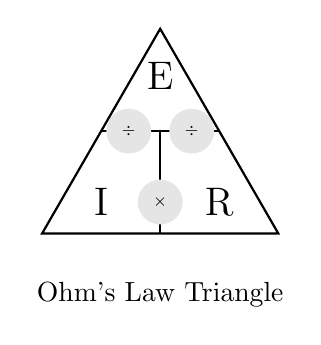
\begin{tikzpicture}
        % Draw the triangle
        \draw[thick] (0,0) -- (3,0) -- (1.5,2.6) -- cycle;
        
        % Add the dividing lines
        \draw[thick] (1.5,0) -- (1.5,1.3);
        \draw[thick] (0.75,1.3) -- (2.25,1.3);
        
        % Add the variables
        \node at (1.5,2.0) {\Large E};  % Voltage at top
        \node at (0.75,0.4) {\Large I}; % Current at bottom left
        \node at (2.25,0.4) {\Large R}; % Resistance at bottom right
        
        % Add multiplication and division symbols in filled circles
        \node[circle, fill=black!10, minimum size=0.02cm] at (1.5,0.4) {\tiny $\times$};  % Multiplication symbol
        \node[circle, fill=black!10, minimum size=0.02cm] at (1.1,1.3) {\tiny $\div$};    % Division symbol
        \node[circle, fill=black!10, minimum size=0.02cm] at (1.9,1.3) {\tiny$\div$};    % Division symbol
        
        % Optional: Add a caption below
        \node[below] at (1.5,-0.5) {Ohm's Law Triangle};
    \end{tikzpicture}
    \caption{Ohm's Law Triangle: To find any value, cover that letter and perform the operation shown between the remaining letters. For voltage (E), multiply I × R. For current (I), divide E ÷ R. For resistance (R), divide E ÷ I.}
    \label{fig:ohms-law-triangle}
\end{figure}

\subsubsection*{Calculating Current}
To calculate current, you need to know the voltage and resistance in the circuit. Using Equation \ref{eq:current}, you can find the current by dividing the voltage by the resistance. For example, if you have a circuit with a 12-volt battery and a 4-ohm resistor, the current would be:

\[
I = \frac{12\,\text{V}}{4\,\Omega} = 3\,\text{A}
\]

\subsubsection*{Calculating Voltage}
If you know the current and resistance, you can calculate the voltage using Equation \ref{eq:ohms-law}. For instance, if a circuit has a current of 2 amperes and a resistance of 5 ohms, the voltage would be:

\[
E = 2\,\text{A} \times 5\,\Omega = 10\,\text{V}
\]

\subsubsection*{Calculating Resistance}
Finally, if you know the voltage and current, you can find the resistance using Equation \ref{eq:resistance}. For example, if a circuit has a voltage of 9 volts and a current of 3 amperes, the resistance would be:

\[
R = \frac{9\,\text{V}}{3\,\text{A}} = 3\,\Omega
\]

\subsubsection*{Series and Parallel Circuits}
In a series circuit, the current is the same through all components, but the voltage across each component can vary. This is because the total resistance in a series circuit is the sum of all individual resistances. On the other hand, in a parallel circuit, the voltage is the same across all components, but the current can vary. The total resistance in a parallel circuit is less than the smallest individual resistance.

\begin{figure}[h!]
    \centering
    % \includegraphics[width=0.8\textwidth]{tech/images/simple-loop-circuit.png}
    \caption{Ohm's Law in a simple circuit}
    \label{fig:ohms-law}
    % Diagram illustrating Ohm's Law with a simple circuit showing voltage, current, and resistance.
\end{figure}

\begin{figure}[h!]
    \centering
    %\includegraphics[width=0.8\textwidth]{figures/series-parallel}

    \caption{Series vs. parallel circuits.}
    \label{fig:series-parallel}
    % Comparison diagram of series and parallel circuits, highlighting differences in current and voltage.
\end{figure}

\begin{table}[h!]
    \centering
    \begin{tabular}{|c|c|}
        \hline
        \textbf{Quantity} & \textbf{Formula} \\
        \hline
        Voltage (\(E\)) & \(E = I \times R\) \\
        Current (\(I\)) & \(I = \frac{E}{R}\) \\
        Resistance (\(R\)) & \(R = \frac{E}{I}\) \\
        \hline
    \end{tabular}
    \caption{Ohm's Law formulas.}
    \label{tab:ohms-law-formulas}
\end{table}

\subsubsection*{Questions}

\begin{tcolorbox}[colback=gray!10!white,colframe=black!75!black,title={T5D01}]
    What formula is used to calculate current in a circuit?
    \begin{enumerate}[label=\Alph*),noitemsep]
        \item \(I = E R\)
        \item \textbf{\(I = E / R\)}
        \item \(I = E + R\)
        \item \(I = E - R\)
    \end{enumerate}
\end{tcolorbox}
The correct formula for calculating current is \(I = E / R\), as shown in Equation \ref{eq:current}. The other options are incorrect because they either multiply, add, or subtract the voltage and resistance, which doesn’t make sense in the context of Ohm’s Law.

\begin{tcolorbox}[colback=gray!10!white,colframe=black!75!black,title={T5D02}]
    What formula is used to calculate voltage in a circuit?
    \begin{enumerate}[label=\Alph*),noitemsep]
        \item \textbf{\(E = I \times R\)}
        \item \(E = I / R\)
        \item \(E = I + R\)
        \item \(E = I - R\)
    \end{enumerate}
\end{tcolorbox}
The correct formula for calculating voltage is \(E = I \times R\), as shown in Equation \ref{eq:ohms-law}. The other options are incorrect because they either divide, add, or subtract the current and resistance, which doesn’t align with Ohm’s Law.

\begin{tcolorbox}[colback=gray!10!white,colframe=black!75!black,title={T5D03}]
    What formula is used to calculate resistance in a circuit?
    \begin{enumerate}[label=\Alph*),noitemsep]
        \item \(R = E \times I\)
        \item \textbf{\(R = E / I\)}
        \item \(R = E + I\)
        \item \(R = E - I\)
    \end{enumerate}
\end{tcolorbox}
The correct formula for calculating resistance is \(R = E / I\), as shown in Equation \ref{eq:resistance}. The other options are incorrect because they either multiply, add, or subtract the voltage and current, which doesn’t follow Ohm’s Law.

\begin{tcolorbox}[colback=gray!10!white,colframe=black!75!black,title={T5D04}]
    What is the resistance of a circuit in which a current of 3 amperes flows when connected to 90 volts?
    \begin{enumerate}[label=\Alph*),noitemsep]
        \item 3 ohms
        \item \textbf{30 ohms}
        \item 93 ohms
        \item 270 ohms
    \end{enumerate}
\end{tcolorbox}
Using Equation \ref{eq:resistance}, the resistance is calculated as \(R = \frac{90\,\text{V}}{3\,\text{A}} = 30\,\Omega\). The other options are incorrect because they either misapply the formula or perform incorrect calculations.

\begin{tcolorbox}[colback=gray!10!white,colframe=black!75!black,title={T5D05}]
    What is the resistance of a circuit for which the applied voltage is 12 volts and the current flow is 1.5 amperes?
    \begin{enumerate}[label=\Alph*),noitemsep]
        \item 18 ohms
        \item 0.125 ohms
        \item \textbf{8 ohms}
        \item 13.5 ohms
    \end{enumerate}
\end{tcolorbox}
Using Equation \ref{eq:resistance}, the resistance is calculated as \(R = \frac{12\,\text{V}}{1.5\,\text{A}} = 8\,\Omega\). The other options are incorrect because they either misapply the formula or perform incorrect calculations.

\begin{tcolorbox}[colback=gray!10!white,colframe=black!75!black,title={T5D06}]
    What is the resistance of a circuit that draws 4 amperes from a 12-volt source?
    \begin{enumerate}[label=\Alph*),noitemsep]
        \item \textbf{3 ohms}
        \item 16 ohms
        \item 48 ohms
        \item 8 ohms
    \end{enumerate}
\end{tcolorbox}
Using Equation \ref{eq:resistance}, the resistance is calculated as \(R = \frac{12\,\text{V}}{4\,\text{A}} = 3\,\Omega\). The other options are incorrect because they either misapply the formula or perform incorrect calculations.

\begin{tcolorbox}[colback=gray!10!white,colframe=black!75!black,title={T5D07}]
    What is the current in a circuit with an applied voltage of 120 volts and a resistance of 80 ohms?
    \begin{enumerate}[label=\Alph*),noitemsep]
        \item 9600 amperes
        \item 200 amperes
        \item 0.667 amperes
        \item \textbf{1.5 amperes}
    \end{enumerate}
\end{tcolorbox}
Using Equation \ref{eq:current}, the current is calculated as \(I = \frac{120\,\text{V}}{80\,\Omega} = 1.5\,\text{A}\). The other options are incorrect because they either misapply the formula or perform incorrect calculations.

\begin{tcolorbox}[colback=gray!10!white,colframe=black!75!black,title={T5D08}]
    What is the current through a 100-ohm resistor connected across 200 volts?
    \begin{enumerate}[label=\Alph*),noitemsep]
        \item 20,000 amperes
        \item 0.5 amperes
        \item \textbf{2 amperes}
        \item 100 amperes
    \end{enumerate}
\end{tcolorbox}
Using Equation \ref{eq:current}, the current is calculated as \(I = \frac{200\,\text{V}}{100\,\Omega} = 2\,\text{A}\). The other options are incorrect because they either misapply the formula or perform incorrect calculations.

\begin{tcolorbox}[colback=gray!10!white,colframe=black!75!black,title={T5D09}]
    What is the current through a 24-ohm resistor connected across 240 volts?
    \begin{enumerate}[label=\Alph*),noitemsep]
        \item 24,000 amperes
        \item 0.1 amperes
        \item \textbf{10 amperes}
        \item 216 amperes
    \end{enumerate}
\end{tcolorbox}
Using Equation \ref{eq:current}, the current is calculated as \(I = \frac{240\,\text{V}}{24\,\Omega} = 10\,\text{A}\). The other options are incorrect because they either misapply the formula or perform incorrect calculations.

\begin{tcolorbox}[colback=gray!10!white,colframe=black!75!black,title={T5D10}]
    What is the voltage across a 2-ohm resistor if a current of 0.5 amperes flows through it?
    \begin{enumerate}[label=\Alph*),noitemsep]
        \item \textbf{1 volt}
        \item 0.25 volts
        \item 2.5 volts
        \item 1.5 volts
    \end{enumerate}
\end{tcolorbox}
Using Equation \ref{eq:ohms-law}, the voltage is calculated as \(E = 0.5\,\text{A} \times 2\,\Omega = 1\,\text{V}\). The other options are incorrect because they either misapply the formula or perform incorrect calculations.

\begin{tcolorbox}[colback=gray!10!white,colframe=black!75!black,title={T5D11}]
    What is the voltage across a 10-ohm resistor if a current of 1 ampere flows through it?
    \begin{enumerate}[label=\Alph*),noitemsep]
        \item 1 volt
        \item \textbf{10 volts}
        \item 11 volts
        \item 9 volts
    \end{enumerate}
\end{tcolorbox}
Using Equation \ref{eq:ohms-law}, the voltage is calculated as \(E = 1\,\text{A} \times 10\,\Omega = 10\,\text{V}\). The other options are incorrect because they either misapply the formula or perform incorrect calculations.

\begin{tcolorbox}[colback=gray!10!white,colframe=black!75!black,title={T5D12}]
    What is the voltage across a 10-ohm resistor if a current of 2 amperes flows through it?
    \begin{enumerate}[label=\Alph*),noitemsep]
        \item 8 volts
        \item 0.2 volts
        \item 12 volts
        \item \textbf{20 volts}
    \end{enumerate}
\end{tcolorbox}
Using Equation \ref{eq:ohms-law}, the voltage is calculated as \(E = 2\,\text{A} \times 10\,\Omega = 20\,\text{V}\). The other options are incorrect because they either misapply the formula or perform incorrect calculations.

\begin{tcolorbox}[colback=gray!10!white,colframe=black!75!black,title={T5D13}]
    In which type of circuit is DC current the same through all components?
    \begin{enumerate}[label=\Alph*),noitemsep]
        \item \textbf{Series}
        \item Parallel
        \item Resonant
        \item Branch
    \end{enumerate}
\end{tcolorbox}
In a series circuit, the current is the same through all components. This is because there’s only one path for the current to flow. In parallel circuits, the current can vary across different branches.

\begin{tcolorbox}[colback=gray!10!white,colframe=black!75!black,title={T5D14}]
    In which type of circuit is voltage the same across all components?
    \begin{enumerate}[label=\Alph*),noitemsep]
        \item Series
        \item \textbf{Parallel}
        \item Resonant
        \item Branch
    \end{enumerate}
\end{tcolorbox}
In a parallel circuit, the voltage is the same across all components. This is because each component is connected directly to the voltage source. In series circuits, the voltage can vary across different components.

\section{Power and Decibels}
\subsection{Decibel Calculations}
\label{subsec:power-db}

Now, let's talk about decibels (dB). Decibels are a logarithmic unit used to express the ratio of two values of a physical quantity, often power or intensity. In radio systems, decibels are used to describe power changes in a way that's easy to understand and compare.

The formula to calculate the decibel value for a power change is:

\begin{equation}
\text{dB} = 10 \log_{10}\left(\frac{P_2}{P_1}\right)
\label{eq:db-calc}
\end{equation}

where \(P_1\) is the initial power and \(P_2\) is the final power. This formula is your best friend when dealing with power changes in radio systems.

\subsubsection*{Examples of Power Changes in Decibels}
Let's look at some examples to make this clearer. Suppose you increase the power from 5 watts to 10 watts. Using equation \ref{eq:db-calc}, we get:

\[
\text{dB} = 10 \log_{10}\left(\frac{10}{5}\right) = 10 \log_{10}(2) \approx 3 \text{ dB}
\]

So, a power increase from 5 watts to 10 watts is approximately 3 dB. Similarly, if you decrease the power from 12 watts to 3 watts, the calculation would be:

\[
\text{dB} = 10 \log_{10}\left(\frac{3}{12}\right) = 10 \log_{10}(0.25) \approx -6 \text{ dB}
\]

This means a power decrease from 12 watts to 3 watts is approximately -6 dB.

\begin{figure}[h]
    \centering
    \begin{minipage}{0.48\textwidth}
        \centering
        \scriptsize
        \begin{tabular}{|c|c||c|c|}
            \hline
            \textbf{Ratio} & \textbf{dB} & \textbf{Ratio} & \textbf{dB} \\
            \hline
            10000 & +40.0 & 1/10000 & -40.0 \\
            1000 & +30.0 & 1/1000 & -30.0 \\
            100 & +20.0 & 1/100 & -20.0 \\
            90 & +19.5 & 1/90 & -19.5 \\
            80 & +19.0 & 1/80 & -19.0 \\
            70 & +18.5 & 1/70 & -18.5 \\
            60 & +17.8 & 1/60 & -17.8 \\
            50 & +17.0 & 1/50 & -17.0 \\
            40 & +16.0 & 1/40 & -16.0 \\
            30 & +14.8 & 1/30 & -14.8 \\
            20 & +13.0 & 1/20 & -13.0 \\
            10 & +10.0 & 1/10 & -10.0 \\
            9 & +9.5 & 1/9 & -9.5 \\
            8 & +9.0 & 1/8 & -9.0 \\
            7 & +8.5 & 1/7 & -8.5 \\
            6 & +7.8 & 1/6 & -7.8 \\
            5 & +7.0 & 1/5 & -7.0 \\
            4 & +6.0 & 1/4 & -6.0 \\
            3 & +4.8 & 1/3 & -4.8 \\
            2 & +3.0 & 1/2 & -3.0 \\
            1 & 0.0 & 1 & 0.0 \\
            \hline
        \end{tabular}
        \captionof{table}{Power Ratios to dB}
        \label{tab:power-db-ratios}
    \end{minipage}%
    \begin{minipage}{0.48\textwidth}
        \centering
        \scriptsize
        \begin{tabular}{|c|c||c|c|}
            \hline
            \textbf{dB} & \textbf{Ratio} & \textbf{dB} & \textbf{Ratio} \\
            \hline
            +20 & 100.0 & -20 & 0.010 \\
            +19 & 79.4 & -19 & 0.013 \\
            +18 & 63.1 & -18 & 0.016 \\
            +17 & 50.1 & -17 & 0.020 \\
            +16 & 39.8 & -16 & 0.025 \\
            +15 & 31.6 & -15 & 0.032 \\
            +14 & 25.1 & -14 & 0.040 \\
            +13 & 20.0 & -13 & 0.050 \\
            +12 & 15.8 & -12 & 0.063 \\
            +11 & 12.6 & -11 & 0.079 \\
            +10 & 10.0 & -10 & 0.100 \\
            +9 & 7.94 & -9 & 0.126 \\
            +8 & 6.31 & -8 & 0.158 \\
            +7 & 5.01 & -7 & 0.200 \\
            +6 & 3.98 & -6 & 0.251 \\
            +5 & 3.16 & -5 & 0.316 \\
            +4 & 2.51 & -4 & 0.398 \\
            +3 & 2.00 & -3 & 0.500 \\
            +2 & 1.58 & -2 & 0.631 \\
            +1 & 1.26 & -1 & 0.794 \\
            0 & 1.00 & 0 & 1.000 \\
            \hline
        \end{tabular}
        \captionof{table}{dB to Power Ratios}
        \label{tab:db-power-ratios}
    \end{minipage}
    \begin{tcolorbox}[colback=gray!10!white,colframe=black!75!black,title={Key Points}]
        Common values to remember:
        \begin{itemize}[noitemsep]            \item Double power (+3 dB) / Half power (-3 dB)
            \item 10 times power (+10 dB) / One-tenth power (-10 dB)
            \item 100 times power (+20 dB) / One-hundredth power (-20 dB)
        \end{itemize}
        \end{tcolorbox}
        \end{figure}

Understanding decibel values is crucial in radio communication. It helps you determine how much power you need to transmit a signal over a certain distance or how much power you can expect to lose due to obstacles. It's like knowing the fuel efficiency of your car—it helps you plan your journey better.


\subsubsection*{Questions}

\begin{tcolorbox}[colback=gray!10!white,colframe=black!75!black,title={T5B09}]
Which decibel value most closely represents a power increase from 5 watts to 10 watts?
\begin{enumerate}[label=\Alph*),noitemsep]
    \item 2 dB
    \item \textbf{3 dB}
    \item 5 dB
    \item 10 dB
\end{enumerate}
\end{tcolorbox}

Using $\text{dB} = 10 \log_{10}(\frac{P_2}{P_1})$:
$\text{dB} = 10 \log_{10}(\frac{10\text{ W}}{5\text{ W}}) = 10 \log_{10}(2) \approx 3\text{ dB}$

\begin{tcolorbox}[colback=gray!10!white,colframe=black!75!black,title={T5B10}]
Which decibel value most closely represents a power decrease from 12 watts to 3 watts?
\begin{enumerate}[label=\Alph*),noitemsep]
    \item -1 dB
    \item -3 dB
    \item \textbf{-6 dB}
    \item -9 dB
\end{enumerate}
\end{tcolorbox}

Using $\text{dB} = 10 \log_{10}(\frac{P_2}{P_1})$:
$\text{dB} = 10 \log_{10}(\frac{3\text{ W}}{12\text{ W}}) = 10 \log_{10}(0.25) \approx -6\text{ dB}$

\begin{tcolorbox}[colback=gray!10!white,colframe=black!75!black,title={T5B11}]
Which decibel value represents a power increase from 20 watts to 200 watts?
\begin{enumerate}[label=\Alph*),noitemsep]
    \item \textbf{10 dB}
    \item 12 dB
    \item 18 dB
    \item 28 dB
\end{enumerate}
\end{tcolorbox}

Using $\text{dB} = 10 \log_{10}(\frac{P_2}{P_1})$:
$\text{dB} = 10 \log_{10}(\frac{200\text{ W}}{20\text{ W}}) = 10 \log_{10}(10) = 10\text{ dB}$

\section{Units and Conversions}
\subsection{Metric Units (k, M, etc.)}
\label{subsec:metric}

When working with radio technology, understanding metric prefixes is like knowing the alphabet before you can read. These prefixes help us express very large or very small numbers in a more manageable way. For example, instead of saying "1,000,000 hertz," we can say "1 megahertz" (1 MHz). This not only saves time but also makes communication clearer, especially when dealing with frequencies, voltages, and currents.

\subsubsection*{Metric Prefixes and Their Significance}
Metric prefixes are like the shorthand of the engineering world. They represent powers of ten, making it easier to work with numbers that would otherwise be unwieldy. For instance, "kilo" (k) stands for $10^3$, "mega" (M) for $10^6$, and "milli" (m) for $10^{-3}$. These prefixes are used across various units, such as volts, amperes, and hertz, to simplify calculations and discussions.

\subsubsection*{Unit Conversions}
Converting between units is a fundamental skill in radio technology. For example, converting amperes to milliamperes involves multiplying by 1,000, since 1 ampere (A) equals 1,000 milliamperes (mA). Similarly, converting hertz to kilohertz involves dividing by 1,000. These conversions are essential when working with different components and systems, ensuring that everything is compatible and functions as intended.

\subsubsection*{Frequency Units in Radio Communications}
Frequency is the heartbeat of radio communications. Understanding units like hertz (Hz), kilohertz (kHz), and megahertz (MHz) is crucial because they define the range of frequencies that radios can transmit and receive. For example, the AM radio band operates in the range of 530 to 1700 kHz, while FM radio operates between 88 and 108 MHz. Knowing how to convert between these units helps in tuning radios and understanding signal propagation.

\subsubsection*{Voltage and Power Conversions}
Voltage and power are also expressed using metric prefixes. For instance, 1 kilovolt (kV) is equal to 1,000 volts (V), and 1 milliwatt (mW) is equal to 0.001 watts (W). These conversions are important when designing circuits or selecting components, as they ensure that the correct voltage and power levels are maintained.

\subsubsection*{Capacitance and Picofarads}
Capacitance, measured in farads (F), often involves very small values, such as picofarads (pF). One picofarad is equal to $10^{-12}$ farads. Understanding these units is essential when working with capacitors, which are used in tuning circuits and filtering signals.

\subsubsection*{Practical Applications of Frequency Conversions}
Frequency conversions are not just theoretical; they have practical applications in radio technology. For example, converting MHz to kHz is necessary when working with different radio bands. Similarly, converting GHz to MHz is important in microwave communications. These conversions ensure that signals are transmitted and received at the correct frequencies, avoiding interference and ensuring clear communication.

% \begin{figure}[htbp]
%     \centering
%     % \includegraphics[width=0.8\textwidth]{metric-prefixes}
%     \caption{Metric Prefixes and Their Values}
%     \label{fig:metric-prefixes}
%     % Diagram showing the relationship between different metric prefixes (kilo, mega, milli, micro, etc.) and their corresponding values.
% \end{figure}

% \begin{figure}[htbp]
%     \centering
%     % \includegraphics[width=0.8\textwidth]{unit-conversion-flowchart}
%     \caption{Unit Conversion Flowchart}
%     \label{fig:unit-conversion-flowchart}
%     % Flowchart illustrating the process of converting between different units of electrical measurements.
% \end{figure}

% \begin{figure}[htbp]
%     \centering
%     % \includegraphics[width=0.8\textwidth]{frequency-units}
%     \caption{Frequency Unit Relationships}
%     \label{fig:frequency-units}
%     % Graph showing the relationship between frequency units (Hz, kHz, MHz, GHz).
% \end{figure}

\begin{table}[htbp]
    \centering
    \caption{Common Metric Prefixes and Electrical Units}
    \label{tab:metric-prefixes}
    \scriptsize
    \begin{tabular}{|c|c|c|c|c|c|c|c|}
        \hline
        Prefix & Symbol & Scientific & Current & Voltage & Resistance & Frequency & Power \\
        & & Notation & (Amperes) & (Volts) & (Ohms) & (Hertz) & (Watts) \\
        \hline
        Tera & T & $10^{12}$ & TA & TV & T$\Omega$ & THz & TW \\
        Giga & G & $10^9$ & GA & GV & G$\Omega$ & GHz & GW \\
        Mega & M & $10^6$ & MA & MV & M$\Omega$ & MHz & MW \\
        Kilo & k & $10^3$ & kA & kV & k$\Omega$ & kHz & kW \\
        \hline
        (unit) & - & $10^0$ & A & V & $\Omega$ & Hz & W \\
        \hline
        milli & m & $10^{-3}$ & mA & mV & m$\Omega$ & mHz & mW \\
        micro & $\mu$ & $10^{-6}$ & $\mu$A & $\mu$V & $\mu\Omega$ & $\mu$Hz & $\mu$W \\
        nano & n & $10^{-9}$ & nA & nV & n$\Omega$ & nHz & nW \\
        pico & p & $10^{-12}$ & pA & pV & p$\Omega$ & pHz & pW \\
        femto & f & $10^{-15}$ & fA & fV & f$\Omega$ & fHz & fW \\
        \hline
    \end{tabular}
\end{table}

\begin{tcolorbox}[colback=gray!10!white,colframe=black!75!black,title={Common Usage}]
Most frequently used combinations in amateur radio:
\begin{itemize}[noitemsep]
    \item Current: mA, A
    \item Voltage: mV, V, kV
    \item Resistance: $\Omega$, k$\Omega$, M$\Omega$
    \item Capacitance: pF, nF, $\mu$F
    \item Inductance: $\mu$H, mH, H
    \item Frequency: Hz, kHz, MHz, GHz
    \item Power: mW, W, kW
\end{itemize}
\end{tcolorbox}

% \begin{table}[htbp]
%     \centering
%     \caption{Unit Conversion Factors}
%     \label{tab:unit-conversion-factors}
%     \begin{tabular}{|c|c|}
%         \hline
%         Conversion & Factor \\
%         \hline
%         1 A to mA & 1,000 \\
%         1 V to kV & 0.001 \\
%         1 W to mW & 1,000 \\
%         1 F to pF & $10^{12}$ \\
%         \hline
%     \end{tabular}
% \end{table}

% \begin{table}[htbp]
%     \centering
%     \caption{Frequency Unit Conversions}
%     \label{tab:frequency-conversions}
%     \begin{tabular}{|c|c|}
%         \hline
%         Conversion & Factor \\
%         \hline
%         1 Hz to kHz & 0.001 \\
%         1 kHz to MHz & 0.001 \\
%         1 MHz to GHz & 0.001 \\
%         \hline
%     \end{tabular}
% \end{table}

\textbf{Questions}

\begin{tcolorbox}[colback=gray!10!white,colframe=black!75!black,title={T5B01}]
    How many milliamperes is 1.5 amperes?
    \begin{enumerate}[label=\Alph*),noitemsep]
        \item 15 milliamperes
        \item 150 milliamperes
        \item \textbf{1500 milliamperes}
        \item 15,000 milliamperes
    \end{enumerate}
\end{tcolorbox}
To convert amperes to milliamperes, multiply by 1,000. Therefore, 1.5 amperes is equal to 1,500 milliamperes. The other options are incorrect because they either under or overestimate the conversion factor.


\begin{tcolorbox}[colback=gray!10!white,colframe=black!75!black,title={T5B03}]
    Which is equal to one kilovolt?
    \begin{enumerate}[label=\Alph*),noitemsep]
        \item One one-thousandth of a volt
        \item One hundred volts
        \item \textbf{One thousand volts}
        \item One million volts
    \end{enumerate}
\end{tcolorbox}
One kilovolt is equal to 1,000 volts. The other options are incorrect because they either under or overestimate the conversion factor.

\begin{tcolorbox}[colback=gray!10!white,colframe=black!75!black,title={T5B04}]
    Which is equal to one microvolt?
    \begin{enumerate}[label=\Alph*),noitemsep]
        \item \textbf{One one-millionth of a volt}
        \item One million volts
        \item One thousand kilovolts
        \item One one-thousandth of a volt
    \end{enumerate}
\end{tcolorbox}
One microvolt is equal to one one-millionth of a volt. The other options are incorrect because they either over or underestimate the conversion factor.


\begin{tcolorbox}[colback=gray!10!white,colframe=black!75!black,title={T5B06}]
    Which is equal to 3000 milliamperes?
    \begin{enumerate}[label=\Alph*),noitemsep]
        \item 0.003 amperes
        \item 0.3 amperes
        \item 3,000,000 amperes
        \item \textbf{3 amperes}
    \end{enumerate}
\end{tcolorbox}
3000 milliamperes is equal to 3 amperes. The other options are incorrect because they either under or overestimate the conversion factor.


\begin{tcolorbox}[colback=gray!10!white,colframe=black!75!black,title={T5B08}]
    Which is equal to 1,000,000 picofarads?
    \begin{enumerate}[label=\Alph*),noitemsep]
        \item 0.001 microfarads
        \item \textbf{1 microfarad}
        \item 1000 microfarads
        \item 1,000,000,000 microfarads
    \end{enumerate}
\end{tcolorbox}
1,000,000 picofarads is equal to 1 microfarad. The other options are incorrect because they either under or overestimate the conversion factor.


\chapter{AC, Impedance, and Circuit Concepts}
\section{AC vs. DC, Frequency, Wavelength}
\subsection{Definitions and Effects}
\label{subsec:ac-basics2}

Let's dive into the fascinating world of electromagnetic waves! These waves are the backbone of radio technology, and understanding their properties is crucial. At their core, electromagnetic waves are composed of two primary components: the electric field and the magnetic field. These fields are perpendicular to each other and to the direction of wave propagation. Imagine them as two dancers moving in perfect harmony, each influencing the other. 

Maxwell's equations describe four fundamental relationships in electromagnetism (and they're like the superhero team of physics - each one has its own special power!):
\begin{itemize}[noitemsep]    \item How electric charges create electric fields (Captain Electric's origin story)
    \item How magnetic fields are created by moving charges and changing electric fields (The Magnetic Marvel's secret technique)
    \item How magnetic fields circulate around electric currents and changing electric fields (The Dynamic Duo's team-up move)
    \item How magnetic poles always come in pairs - nature's way of saying "you complete me" (no lonely magnetic monopoles allowed!)
\end{itemize}

Now, let's talk about polarization. Polarization refers to the orientation of the electric field as the wave travels. If the electric field oscillates in a single plane, the wave is said to be linearly polarized. If the electric field rotates as the wave propagates, it can be circularly or elliptically polarized. The orientation of the electric field determines the polarization state, which is crucial for applications like satellite communication and radar systems.

\begin{figure}[h]
    \centering
    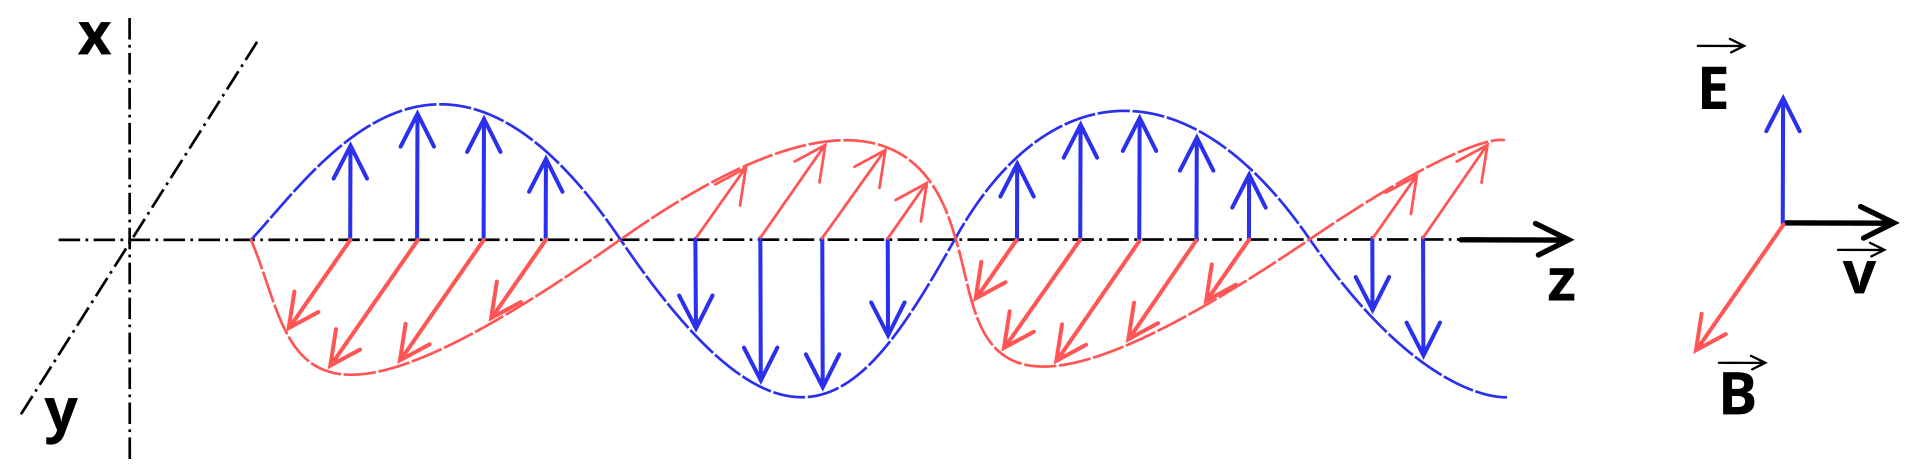
\includegraphics[width=0.8\textwidth]{tech/images/em-wave.png}
    \caption{Relationship between electric and magnetic fields in an electromagnetic wave. The electric field (E) and magnetic field (B) are perpendicular to each other and to the direction of wave propagation. As one field increases, the other follows 90 degrees later in space (like a synchronized dance where one partner bows while the other steps sideways). The wave's energy alternates between electric and magnetic fields as it travels through space, with both fields reaching their maximum and minimum values at different points.}
    \label{fig:em-wave}
    % Image prompt: Diagram showing the relationship between electric and magnetic fields in an electromagnetic wave. The electric field (E) and magnetic field (B) should be shown as perpendicular vectors, with the wave propagating in a direction perpendicular to both.
\end{figure}

\begin{figure}[h]
    \centering
    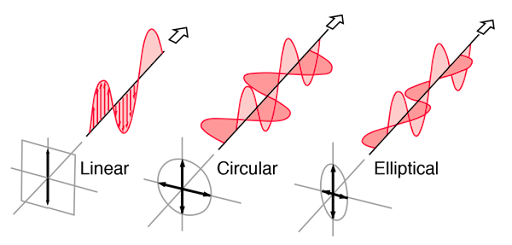
\includegraphics[width=0.8\textwidth]{tech/images/polarization.png}
    \caption{Radio wave polarization determined by the orientation of the electric field. Linear polarization occurs when the electric field oscillates in a single fixed plane (like a jump rope moving up and down). Circular polarization happens when the electric field rotates uniformly around the direction of propagation (like a spiral staircase). Elliptical polarization is similar to circular, but the field strength varies during rotation (imagine squishing that spiral staircase slightly).}
    \label{fig:polarization}
    % Image prompt: Illustration of radio wave polarization showing the orientation of the electric field. The electric field should be shown oscillating in different planes for linear, circular, and elliptical polarization.
\end{figure}

In summary, the electric and magnetic fields are the yin and yang of electromagnetic waves. They work together to create the waves that carry information across vast distances. Understanding their relationship and the concept of polarization is essential for anyone working in radio technology. So, next time you tune into your favorite radio station, remember the intricate dance of electric and magnetic fields that makes it all possible!

\begin{table}[h]
    \centering
    \begin{tabular}{|c|c|c|}
        \hline
        \textbf{Band} & \textbf{Frequency Range} & \textbf{Wavelength Range} \\
        \hline
        HF & 3 MHz to 30 MHz & 100 m to 10 m \\
        VHF & 30 MHz to 300 MHz & 10 m to 1 m \\
        UHF & 300 MHz to 3 GHz & 1 m to 10 cm \\
        SHF & 3 GHz to 30 GHz & 10 cm to 1 cm \\
        EHF & 30 GHz to 300 GHz & 1 cm to 1 mm \\
        \hline
    \end{tabular}
    \caption{Frequency and wavelength ranges for radio frequency bands.}
    \label{tab:frequency-ranges}
\end{table}

\subsection{Frequency \& Wavelength Calculations}
\label{subsec:freq-wavelength}

Radio waves are fascinating, aren't they? They zip through space at the speed of light, carrying information across vast distances. But how fast is that, exactly? Well, in free space, radio waves travel at approximately 300,000,000 meters per second. That's fast enough to circle the Earth about 7.5 times in one second! This speed is crucial in radio communication because it determines how quickly signals can travel from one point to another.

Now, let's talk about the relationship between wavelength and frequency. These two are inversely related, meaning as one increases, the other decreases. The formula to convert frequency to wavelength is:

\begin{equation}
\lambda = \frac{c}{f}
\label{eq:wavelength}
\end{equation}

where \(\lambda\) is the wavelength in meters, \(c\) is the speed of light (approximately 300,000,000 meters per second), and \(f\) is the frequency in hertz. For example, if you have a frequency of 150 MHz, the wavelength would be:

\[
\lambda = \frac{300,000,000}{150,000,000} = 2 \text{ meters}
\]

Amateur radio bands are often identified by both their frequency and their approximate wavelength. For instance, the 2-meter band is a popular VHF band used by amateur radio operators. This dual identification helps in understanding the practical applications and limitations of different frequency ranges.

Speaking of frequency ranges, let's break down the VHF, UHF, and HF bands:

\begin{itemize}[noitemsep]    \item \textbf{VHF (Very High Frequency)}: 30 MHz to 300 MHz. This range is commonly used for FM radio, television broadcasting, and two-way land mobile radio systems.
    \item \textbf{UHF (Ultra High Frequency)}: 300 MHz to 3000 MHz. UHF is used for television broadcasting, mobile phones, and Wi-Fi.
    \item \textbf{HF (High Frequency)}: 3 MHz to 30 MHz. HF is known for its ability to communicate over long distances, making it ideal for international broadcasting and maritime communication.
\end{itemize}

The unit of frequency is the hertz (Hz), named after Heinrich Hertz, who first demonstrated the existence of electromagnetic waves. One hertz represents one cycle per second. This unit is essential in describing how often an alternating current completes a full cycle, which is directly related to the frequency of the radio wave.


\begin{table}[h]
    \centering
    \begin{tabular}{|c|c|}
        \hline
        \textbf{Band} & \textbf{Frequency Range} \\
        \hline
        VHF & 30 MHz to 300 MHz \\
        UHF & 300 MHz to 3000 MHz \\
        HF & 3 MHz to 30 MHz \\
        \hline
    \end{tabular}
    \caption{Frequency ranges for VHF, UHF, and HF bands.}
    \label{tab:frequency-ranges}
\end{table}

\subsubsection*{Questions}

\begin{tcolorbox}[colback=gray!10!white,colframe=black!75!black,title={T3B01}]
What is the relationship between the electric and magnetic fields of an electromagnetic wave?
\begin{enumerate}[label=\Alph*),noitemsep]
    \item They travel at different speeds
    \item They are in parallel
    \item They revolve in opposite directions
    \item \textbf{They are at right angles}
\end{enumerate}
\end{tcolorbox}

The electric and magnetic fields of an electromagnetic wave are perpendicular to each other and to the direction of wave propagation. This orthogonal relationship is fundamental to the nature of electromagnetic waves.

\begin{tcolorbox}[colback=gray!10!white,colframe=black!75!black,title={T3B02}]
What property of a radio wave defines its polarization?
\begin{enumerate}[label=\Alph*),noitemsep]
    \item \textbf{The orientation of the electric field}
    \item The orientation of the magnetic field
    \item The ratio of the energy in the magnetic field to the energy in the electric field
    \item The ratio of the velocity to the wavelength
\end{enumerate}
\end{tcolorbox}

Polarization refers to the orientation of the electric field of the radio wave. This orientation can be horizontal, vertical, or circular, depending on the application.

\begin{tcolorbox}[colback=gray!10!white,colframe=black!75!black,title={T3B03}]
What are the two components of a radio wave?
\begin{enumerate}[label=\Alph*),noitemsep]
    \item Impedance and reactance
    \item Voltage and current
    \item \textbf{Electric and magnetic fields}
    \item Ionizing and non-ionizing radiation
\end{enumerate}
\end{tcolorbox}

A radio wave consists of oscillating electric and magnetic fields. These fields propagate through space, carrying energy and information.

\begin{tcolorbox}[colback=gray!10!white,colframe=black!75!black,title={T3B04}]
What is the velocity of a radio wave traveling through free space?
\begin{enumerate}[label=\Alph*),noitemsep]
    \item \textbf{Speed of light}
    \item Speed of sound
    \item Speed inversely proportional to its wavelength
    \item Speed that increases as the frequency increases
\end{enumerate}
\end{tcolorbox}

In free space, radio waves travel at the speed of light, which is approximately 300,000,000 meters per second.

\begin{tcolorbox}[colback=gray!10!white,colframe=black!75!black,title={T3B05}]
What is the relationship between wavelength and frequency?
\begin{enumerate}[label=\Alph*),noitemsep]
    \item Wavelength gets longer as frequency increases
    \item \textbf{Wavelength gets shorter as frequency increases}
    \item Wavelength and frequency are unrelated
    \item Wavelength and frequency increase as path length increases
\end{enumerate}
\end{tcolorbox}

Wavelength and frequency are inversely related. As frequency increases, wavelength decreases, and vice versa.

\begin{tcolorbox}[colback=gray!10!white,colframe=black!75!black,title={T3B06}]
What is the formula for converting frequency to approximate wavelength in meters?
\begin{enumerate}[label=\Alph*),noitemsep]
    \item Wavelength in meters equals frequency in hertz multiplied by 300
    \item Wavelength in meters equals frequency in hertz divided by 300
    \item Wavelength in meters equals frequency in megahertz divided by 300
    \item \textbf{Wavelength in meters equals 300 divided by frequency in megahertz}
\end{enumerate}
\end{tcolorbox}

The formula \(\lambda = \frac{300}{f}\) (where \(f\) is in MHz) is a quick way to estimate wavelength in meters.

\begin{tcolorbox}[colback=gray!10!white,colframe=black!75!black,title={T3B07}]
In addition to frequency, which of the following is used to identify amateur radio bands?
\begin{enumerate}[label=\Alph*),noitemsep]
    \item \textbf{The approximate wavelength in meters}
    \item Traditional letter/number designators
    \item Channel numbers
    \item All these choices are correct
\end{enumerate}
\end{tcolorbox}

Amateur radio bands are often identified by their approximate wavelength in meters, which helps in understanding their practical use.

\begin{tcolorbox}[colback=gray!10!white,colframe=black!75!black,title={T3B08}]
What frequency range is referred to as VHF?
\begin{enumerate}[label=\Alph*),noitemsep]
    \item 30 kHz to 300 kHz
    \item \textbf{30 MHz to 300 MHz}
    \item 300 kHz to 3000 kHz
    \item 300 MHz to 3000 MHz
\end{enumerate}
\end{tcolorbox}

VHF stands for Very High Frequency and covers the range from 30 MHz to 300 MHz.

\begin{tcolorbox}[colback=gray!10!white,colframe=black!75!black,title={T3B09}]
What frequency range is referred to as UHF?
\begin{enumerate}[label=\Alph*),noitemsep]
    \item 30 to 300 kHz
    \item 30 to 300 MHz
    \item 300 to 3000 kHz
    \item \textbf{300 to 3000 MHz}
\end{enumerate}
\end{tcolorbox}

UHF, or Ultra High Frequency, ranges from 300 MHz to 3000 MHz.

\begin{tcolorbox}[colback=gray!10!white,colframe=black!75!black,title={T3B10}]
What frequency range is referred to as HF?
\begin{enumerate}[label=\Alph*),noitemsep]
    \item 300 to 3000 MHz
    \item 30 to 300 MHz
    \item \textbf{3 to 30 MHz}
    \item 300 to 3000 kHz
\end{enumerate}
\end{tcolorbox}

HF, or High Frequency, spans from 3 MHz to 30 MHz and is known for its long-distance communication capabilities.

\begin{tcolorbox}[colback=gray!10!white,colframe=black!75!black,title={T3B11}]
What is the approximate velocity of a radio wave in free space?
\begin{enumerate}[label=\Alph*),noitemsep]
    \item 150,000 meters per second
    \item \textbf{300,000,000 meters per second}
    \item 300,000,000 miles per hour
    \item 150,000 miles per hour
\end{enumerate}
\end{tcolorbox}

Radio waves travel at the speed of light, which is approximately 300,000,000 meters per second in free space.

\begin{tcolorbox}[colback=gray!10!white,colframe=black!75!black,title={T5A06}]
What is the unit of frequency?
\begin{enumerate}[label=\Alph*),noitemsep]
    \item \textbf{Hertz}
    \item Henry
    \item Farad
    \item Tesla
\end{enumerate}
\end{tcolorbox}

The unit of frequency is the hertz (Hz), named after Heinrich Hertz.

\begin{tcolorbox}[colback=gray!10!white,colframe=black!75!black,title={T5A12}]
What describes the number of times per second that an alternating current makes a complete cycle?
\begin{enumerate}[label=\Alph*),noitemsep]
    \item Pulse rate
    \item Speed
    \item Wavelength
    \item \textbf{Frequency}
\end{enumerate}
\end{tcolorbox}

Frequency is the term used to describe how many times per second an alternating current completes a full cycle.

\section{Capacitance, Inductance, and Impedance}
\subsection{Capacitors}
\label{subsec:capacitors}

In this section, we'll dive into the fascinating world of capacitors. If you've ever wondered how energy can be stored in an electric field, you're in the right place. Let's start by understanding the concept of capacitance and its role in storing energy.

\subsubsection*{Capacitance: Storing Energy in an Electric Field}

Capacitance is the ability of a system to store energy in an electric field. Think of it as a tiny energy reservoir that can hold onto electrical energy until it's needed. This is particularly useful in circuits where you might need a quick burst of energy, like in a camera flash or a defibrillator.

The basic idea is that when you apply a voltage across a capacitor, it stores energy in the form of an electric field between its plates. The amount of energy stored depends on the capacitance of the capacitor, which is measured in farads (F). The higher the capacitance, the more energy it can store.

Mathematically, the energy \( E \) stored in a capacitor is given by:
\begin{equation}
    E = \frac{1}{2} C V^2
\end{equation}
where \( C \) is the capacitance and \( V \) is the voltage across the capacitor.

\subsubsection*{The Farad: Unit of Capacitance}

The unit of capacitance is the farad, named after the English physicist Michael Faraday. One farad is defined as the capacitance of a capacitor that stores one coulomb of charge when one volt is applied across it. In practical terms, a farad is a pretty large unit, so you'll often see capacitors measured in microfarads (\( \mu F \)), nanofarads (\( nF \)), or picofarads (\( pF \)).

The farad is crucial in electrical circuits because it determines how much energy a capacitor can store and how quickly it can release that energy. For example, in a timing circuit, the capacitance value will directly affect the time constant of the circuit.


\begin{table}[h]
    \centering
    \begin{tabular}{|c|c|}
        \hline
        \textbf{Capacitor Type} & \textbf{Capacitance Range} \\
        \hline
        Ceramic & 1 pF to 100 \(\mu F\) \\
        Electrolytic & 1 \(\mu F\) to 1 F \\
        Tantalum & 1 \(\mu F\) to 100 \(\mu F\) \\
        Film & 1 pF to 100 \(\mu F\) \\
        \hline
    \end{tabular}
    \caption{Comparison of capacitance values for various capacitor types.}
    \label{tab:capacitance-values}
\end{table}

\subsubsection{Questions}

\begin{tcolorbox}[colback=gray!10!white,colframe=black!75!black,title={T5C01}]
    What describes the ability to store energy in an electric field?
    \begin{enumerate}[label=\Alph*),noitemsep]
        \item Inductance
        \item Resistance
        \item Tolerance
        \item \textbf{Capacitance}
    \end{enumerate}
\end{tcolorbox}

Capacitance is the correct answer because it directly relates to the ability to store energy in an electric field. Inductance (A) is related to magnetic fields, resistance (B) is about opposing current flow, and tolerance (C) refers to the allowable variation in a component's value.

\begin{tcolorbox}[colback=gray!10!white,colframe=black!75!black,title={T5C02}]
    What is the unit of capacitance?
    \begin{enumerate}[label=\Alph*),noitemsep]
        \item \textbf{The farad}
        \item The ohm
        \item The volt
        \item The henry
    \end{enumerate}
\end{tcolorbox}

The farad (A) is the unit of capacitance, named after Michael Faraday. The ohm (B) is the unit of resistance, the volt (C) is the unit of voltage, and the henry (D) is the unit of inductance.

That's it for capacitors! Now you know how they store energy and why the farad is such an important unit in electrical circuits. Next time you see a capacitor, you'll appreciate the tiny electric field powerhouse it truly is.

\subsection{Inductors}
\label{subsec:inductors}

Inductors are fascinating little components that play a crucial role in electrical circuits. At their core, inductors are all about storing energy in a magnetic field. This ability is known as \textbf{inductance}. When current flows through an inductor, it generates a magnetic field around it. The energy stored in this magnetic field can be released back into the circuit when the current changes, making inductors essential in applications like filtering, tuning, and energy storage.

The unit of inductance is the \textbf{henry} (H), named after the American scientist Joseph Henry. One henry is defined as the inductance of a circuit in which an electromotive force of one volt is produced when the current in the circuit changes at a rate of one ampere per second. In simpler terms, the henry tells us how much magnetic field an inductor can generate for a given current. It's like the inductor's way of saying, "Hey, I can store this much energy in my magnetic field!"

% \begin{figure}[h]
%     \centering
%     % \includegraphics[width=0.8\textwidth]{inductor-circuit.svg}
%     \caption{Inductor in a circuit with magnetic field representation.}
%     \label{fig:inductor-circuit}
%     % Diagram showing an inductor in a circuit and its magnetic field. The inductor is represented as a coil, and the magnetic field lines are shown surrounding it, illustrating the energy storage mechanism.
% \end{figure}

\begin{table}[h]
    \centering
    \begin{tabular}{|c|c|}
        \hline
        \textbf{Inductor Type} & \textbf{Inductance (H)} \\
        \hline
        Air-core & 0.001 - 0.1 \\
        Iron-core & 0.1 - 10 \\
        Ferrite-core & 0.01 - 1 \\
        Toroidal & 0.1 - 100 \\
        \hline
    \end{tabular}
    \caption{Comparison of inductance values for various inductor types.}
    \label{tab:inductance-values}
\end{table}

\subsubsection{Questions}

\begin{tcolorbox}[colback=gray!10!white,colframe=black!75!black,title={T5C03}]
    What describes the ability to store energy in a magnetic field?
    \begin{enumerate}[label=\Alph*),noitemsep]
        \item Admittance
        \item Capacitance
        \item Resistance
        \item \textbf{Inductance}
    \end{enumerate}
\end{tcolorbox}

Inductance is the property that allows an inductor to store energy in a magnetic field. Capacitance, on the other hand, stores energy in an electric field, while resistance dissipates energy as heat. Admittance is a measure of how easily a circuit allows current to flow, but it doesn't directly relate to energy storage in a magnetic field.

\begin{tcolorbox}[colback=gray!10!white,colframe=black!75!black,title={T5C04}]
    What is the unit of inductance?
    \begin{enumerate}[label=\Alph*),noitemsep]
        \item The coulomb
        \item The farad
        \item \textbf{The henry}
        \item The ohm
    \end{enumerate}
\end{tcolorbox}

The henry is the unit of inductance, named after Joseph Henry. The coulomb is the unit of electric charge, the farad is the unit of capacitance, and the ohm is the unit of resistance. So, if you're talking about inductance, you're talking about henries!

\subsection{Impedance, Reactance, etc.}
\label{subsec:imp-react}

In this section, we’ll dive into the fascinating world of impedance and reactance. If you’ve ever wondered why your AC circuits behave differently from DC circuits, you’re in the right place. Let’s start by understanding what impedance is and why it’s such a big deal in AC circuits.

\subsubsection*{What is Impedance?}
Impedance is the opposition that a circuit presents to alternating current (AC). Think of it as the AC version of resistance, but with a twist. While resistance opposes DC current, impedance takes into account not just resistance but also reactance, which is the opposition caused by inductors and capacitors. Mathematically, impedance \( Z \) is represented as:
\begin{equation}
    Z = R + jX
\end{equation}
where \( R \) is the resistance, \( X \) is the reactance, and \( j \) is the imaginary unit (because, yes, AC circuits love to get complex).

\subsubsection*{The Unit of Impedance: The Ohm}
Just like resistance, impedance is measured in ohms (\( \Omega \)). This makes sense because impedance is essentially the AC equivalent of resistance. So, when you see a circuit component with an impedance of 50 ohms, it means it opposes AC current flow with a magnitude of 50 ohms. Simple, right?

\subsubsection*{Impedance vs. Reactance}
Now, let’s clear up a common confusion: the difference between impedance and reactance. Reactance is a component of impedance and is caused by inductors and capacitors. Inductive reactance (\( X_L \)) and capacitive reactance (\( X_C \)) are given by:
\begin{equation}
    X_L = 2\pi f L
\end{equation}
\begin{equation}
    X_C = \frac{1}{2\pi f C}
\end{equation}
where \( f \) is the frequency, \( L \) is the inductance, and \( C \) is the capacitance. Impedance, on the other hand, is the combination of resistance and reactance, as shown in equation (1).

\begin{figure}[h]
    \centering
    % \includegraphics{impedance-circuit.svg} % Placeholder for the image
    \caption{Impedance in an AC circuit. The diagram shows how impedance combines resistance and reactance to oppose AC current flow.}
    \label{fig:impedance-circuit}
\end{figure}

\begin{table}[h]
    \centering
    \begin{tabular}{|c|c|}
        \hline
        \textbf{Component} & \textbf{Impedance} \\
        \hline
        Resistor & \( R \) \\
        Inductor & \( jX_L \) \\
        Capacitor & \( -jX_C \) \\
        \hline
    \end{tabular}
    \caption{Comparison of impedance values for various circuit components.}
    \label{tab:impedance-values}
\end{table}

\subsubsection*{Questions}
\begin{tcolorbox}[colback=gray!10!white,colframe=black!75!black,title={T5C05}]
    What is the unit of impedance?
    \begin{enumerate}[label=\Alph*),noitemsep]
        \item The volt
        \item The ampere
        \item The coulomb
        \item \textbf{The ohm}
    \end{enumerate}
\end{tcolorbox}
The unit of impedance is the ohm (\( \Omega \)), just like resistance. This is because impedance is essentially the AC equivalent of resistance, and both are measures of opposition to current flow.

\begin{tcolorbox}[colback=gray!10!white,colframe=black!75!black,title={T5C12}]
    What is impedance?
    \begin{enumerate}[label=\Alph*),noitemsep]
        \item \textbf{The opposition to AC current flow}
        \item The inverse of resistance
        \item The Q or Quality Factor of a component
        \item The power handling capability of a component
    \end{enumerate}
\end{tcolorbox}
Impedance is the opposition to AC current flow, combining both resistance and reactance. The other options are incorrect because impedance is not the inverse of resistance, nor is it related to the Quality Factor or power handling capability.

\begin{tcolorbox}[colback=gray!10!white,colframe=black!75!black,title={T5C13}]
    What is the abbreviation for kilohertz?
    \begin{enumerate}[label=\Alph*),noitemsep]
        \item KHZ
        \item khz
        \item khZ
        \item \textbf{kHz}
    \end{enumerate}
\end{tcolorbox}
The correct abbreviation for kilohertz is kHz. The lowercase 'k' stands for kilo, and the uppercase 'Hz' stands for hertz. The other options are incorrect due to improper capitalization or letter order.

\subsection{RF and Frequency Abbreviations}
\label{subsec:rf-abbrev}

In this section, we'll dive into some of the most common abbreviations you'll encounter in the world of radio technology. Don't worry, we'll keep it light and fun—no need to panic if you're not a math whiz or a physics guru. We'll start with the basics and build up from there.

\subsubsection*{What is RF?}

First up, let's talk about \textbf{RF}. No, it's not short for "Really Fun" (although radio can be pretty fun). RF stands for \textbf{Radio Frequency}, and it refers to the range of electromagnetic signals used for wireless communication. These signals can be anything from the low-frequency waves used in AM radio to the high-frequency waves used in satellite communications. Essentially, RF is the backbone of all wireless communication, from your Wi-Fi router to your favorite FM radio station.

\subsubsection*{Megahertz and Kilohertz}

Next, let's tackle the abbreviations for frequency measurements. You've probably heard of \textbf{MHz} and \textbf{kHz}, but what do they actually mean? 

- \textbf{MHz} stands for \textbf{Megahertz}, which is a unit of frequency equal to one million hertz. It's commonly used to describe the frequency of radio waves, computer processors, and even some types of light.
  
- \textbf{kHz} stands for \textbf{Kilohertz}, which is a unit of frequency equal to one thousand hertz. This is often used to describe lower-frequency signals, like those used in AM radio.

Both of these units are crucial for understanding how different types of signals are transmitted and received. For example, when you tune your radio to 98.5 FM, you're actually tuning it to 98.5 MHz.

\begin{figure}[h]
    \centering
    % \includegraphics[width=0.8\textwidth]{frequency-spectrum}
    \caption{Frequency spectrum with RF, MHz, and kHz labeled.}
    \label{fig:frequency-spectrum}
    % Prompt: Diagram showing the frequency spectrum with RF, MHz, and kHz labeled.
\end{figure}

\begin{table}[h]
    \centering
    \begin{tabular}{|c|c|}
        \hline
        \textbf{Abbreviation} & \textbf{Meaning} \\
        \hline
        RF & Radio Frequency \\
        MHz & Megahertz \\
        kHz & Kilohertz \\
        \hline
    \end{tabular}
    \caption{Common RF and frequency abbreviations.}
    \label{tab:rf-abbreviations}
\end{table}

\subsubsection{Questions}

\begin{tcolorbox}[colback=gray!10!white,colframe=black!75!black,title={T5C06}]
    What does the abbreviation “RF” mean?
    \begin{enumerate}[label=\Alph*),noitemsep]
        \item \textbf{Radio frequency signals of all types}
        \item The resonant frequency of a tuned circuit
        \item The real frequency transmitted as opposed to the apparent frequency
        \item Reflective force in antenna transmission lines
    \end{enumerate}
\end{tcolorbox}

RF stands for Radio Frequency, which encompasses all types of radio frequency signals used in wireless communication. The other options are either incorrect or unrelated to the abbreviation RF.

\begin{tcolorbox}[colback=gray!10!white,colframe=black!75!black,title={T5C07}]
    What is the abbreviation for megahertz?
    \begin{enumerate}[label=\Alph*),noitemsep]
        \item MH
        \item mh
        \item Mhz
        \item \textbf{MHz}
    \end{enumerate}
\end{tcolorbox}

The correct abbreviation for megahertz is \textbf{MHz}. The other options either use incorrect capitalization or incorrect lettering, which can lead to confusion in technical contexts.

\subsection{Calculating Power with Voltage/Current}
\label{subsec:calc-power}

In this section, we'll dive into the world of electrical power calculations. Don't worry, it's not as shocking as it sounds! (Pun intended.) We'll start by understanding the basic formula for calculating power in a DC circuit and then work through some examples to solidify your understanding.

\subsubsection*{The Power Formula}
The formula for calculating electrical power \( P \) in a DC circuit is straightforward:
\begin{equation}
    P = I \times E
    \label{eq:power-formula}
\end{equation}
where:
\begin{itemize}
    \item \( P \) is the power in watts (W),
    \item \( I \) is the current in amperes (A),
    \item \( E \) is the voltage in volts (V).
\end{itemize}

This equation tells us that power is the product of current and voltage. So, if you know the voltage across a component and the current flowing through it, you can easily calculate the power being delivered.

\subsubsection*{Examples of Power Calculations}
Let's put this formula to work with some examples. Suppose you have a DC circuit with a voltage of 13.8 volts and a current of 10 amperes. Using the power formula:
\begin{equation}
    P = 10 \, \text{A} \times 13.8 \, \text{V} = 138 \, \text{W}
    \label{eq:power-example1}
\end{equation}
So, the power delivered is 138 watts. Easy, right?

Now, let's try another example. If you have a voltage of 12 volts and a current of 2.5 amperes:
\begin{equation}
    P = 2.5 \, \text{A} \times 12 \, \text{V} = 30 \, \text{W}
    \label{eq:power-example2}
\end{equation}
Here, the power delivered is 30 watts.

\subsubsection*{Relationship Between Power, Voltage, and Current}
The relationship between power, voltage, and current is fundamental in electrical circuits. As you can see from the formula, power increases with either an increase in voltage or current. This means that if you want to deliver more power, you can either increase the voltage or the current (or both, if you're feeling adventurous).

\begin{figure}[h]
    \centering
    % \includegraphics[width=0.8\textwidth]{dc-circuit.svg}
    \caption{Simple DC circuit with voltage, current, and power labeled.}
    \label{fig:dc-circuit}
    % Prompt: Diagram showing a simple DC circuit with voltage, current, and power labeled.
\end{figure}

\begin{table}[h]
    \centering
    \begin{tabular}{|c|c|c|}
        \hline
        Voltage (V) & Current (A) & Power (W) \\
        \hline
        13.8 & 10 & 138 \\
        12 & 2.5 & 30 \\
        12 & 10 & 120 \\
        \hline
    \end{tabular}
    \caption{Power calculations for various voltage and current values.}
    \label{tab:power-calculations}
\end{table}

\subsubsection*{Questions}
\begin{tcolorbox}[colback=gray!10!white,colframe=black!75!black,title={T5C08}]
    What is the formula used to calculate electrical power (P) in a DC circuit?
    \begin{enumerate}[label=\Alph*),noitemsep]
        \item \( P = I E \)
        \item \( P = E / I \)
        \item \( P = E - I \)
        \item \( P = I + E \)
    \end{enumerate}
\end{tcolorbox}
The formula for calculating electrical power in a DC circuit is \( P = I E \). This is derived from the basic relationship between power, voltage, and current. The other options are incorrect because they either involve incorrect operations or do not represent the correct relationship between the variables.

\begin{tcolorbox}[colback=gray!10!white,colframe=black!75!black,title={T5C09}]
    How much power is delivered by a voltage of 13.8 volts DC and a current of 10 amperes?
    \begin{enumerate}[label=\Alph*),noitemsep]
        \item \textbf{138 watts}
        \item 0.7 watts
        \item 23.8 watts
        \item 3.8 watts
    \end{enumerate}
\end{tcolorbox}
Using the power formula \( P = I E \), we calculate \( P = 10 \, \text{A} \times 13.8 \, \text{V} = 138 \, \text{W} \). The other options are incorrect because they do not match the result of this calculation.

\begin{tcolorbox}[colback=gray!10!white,colframe=black!75!black,title={T5C10}]
    How much power is delivered by a voltage of 12 volts DC and a current of 2.5 amperes?
    \begin{enumerate}[label=\Alph*),noitemsep]
        \item 4.8 watts
        \item \textbf{30 watts}
        \item 14.5 watts
        \item 0.208 watts
    \end{enumerate}
\end{tcolorbox}
Using the power formula \( P = I E \), we calculate \( P = 2.5 \, \text{A} \times 12 \, \text{V} = 30 \, \text{W} \). The other options are incorrect because they do not match the result of this calculation.

\begin{tcolorbox}[colback=gray!10!white,colframe=black!75!black,title={T5C11}]
    How much current is required to deliver 120 watts at a voltage of 12 volts DC?
    \begin{enumerate}[label=\Alph*),noitemsep]
        \item 0.1 amperes
        \item \textbf{10 amperes}
        \item 12 amperes
        \item 132 amperes
    \end{enumerate}
\end{tcolorbox}
To find the current, we rearrange the power formula to \( I = P / E \). Plugging in the values, \( I = 120 \, \text{W} / 12 \, \text{V} = 10 \, \text{A} \). The other options are incorrect because they do not match the result of this calculation.

\chapter{Electronic and Electrical Components}
\section{Resistors, Capacitors, Inductors}
\subsection{Basics}
\label{subsec:basics-passive}

Let's dive into the fundamental components that make up the backbone of any electronic circuit. These components are like the essential workers of the electronics world—often overlooked but absolutely essential. We'll start with resistors, capacitors, inductors, and switches, and then move on to some battery chemistry basics. By the end of this section, you'll have a solid understanding of how these components work and why they're so important.



\begin{figure}[h!]
    \centering
    \footnotesize
    \begin{tabular}{ccccc}
        % Row 1 - Resistive and Protection Components
        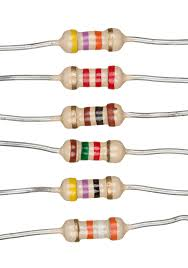
\includegraphics[width=0.11\textwidth]{images/resistor} &
        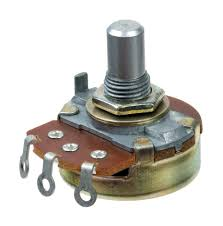
\includegraphics[width=0.11\textwidth]{images/potentiometer} &
        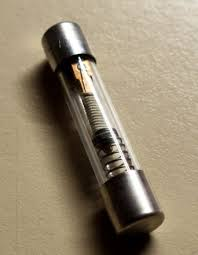
\includegraphics[width=0.11\textwidth]{images/fuse} &
        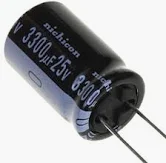
\includegraphics[width=0.11\textwidth]{images/capacitor} &
        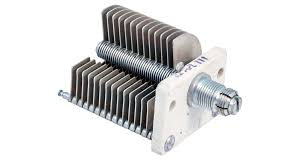
\includegraphics[width=0.11\textwidth]{images/variable-capacitor} \\
        Through-hole Resistor & Potentiometer & Glass Fuse & Ceramic Capacitor & Variable Capacitor \\[2em]
        % Row 2 - Inductors and Switches
        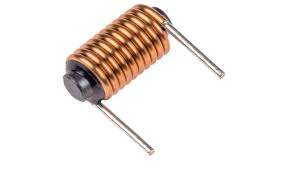
\includegraphics[width=0.11\textwidth]{images/inductor} &
        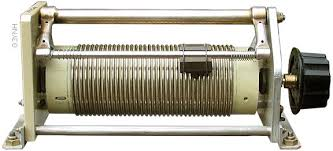
\includegraphics[width=0.11\textwidth]{images/variable-inductor} &
        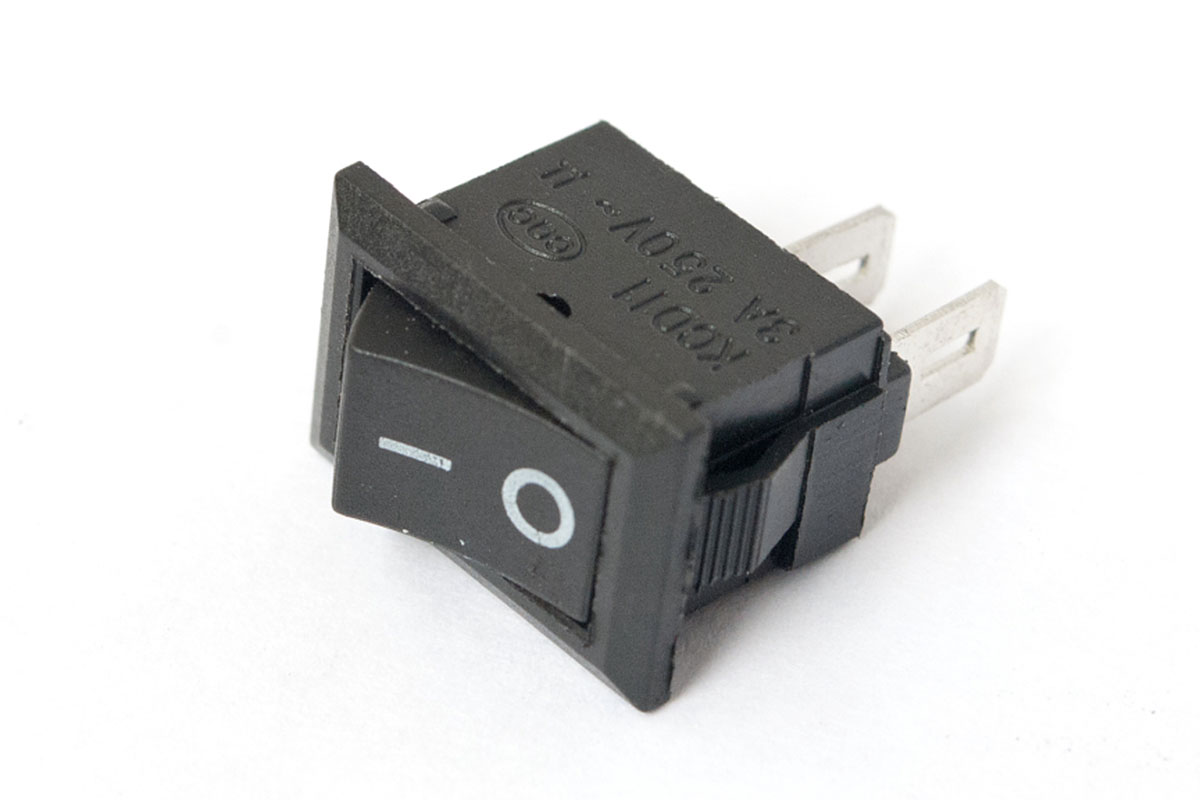
\includegraphics[width=0.11\textwidth]{images/spst} &
        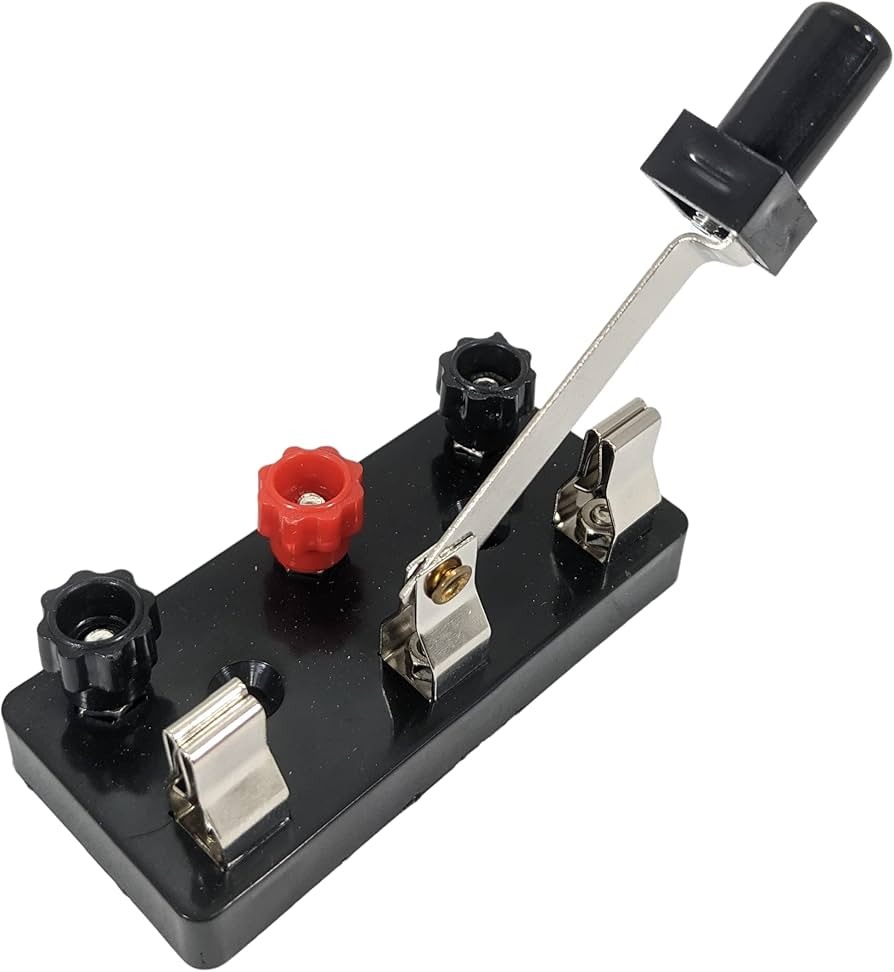
\includegraphics[width=0.11\textwidth]{images/spdt} & \\
        Toroid Inductor & Variable Inductor & SPST Switch & SPDT Switch & \\
    \end{tabular}
    \caption{Common electronic components used in radio circuits. Top row: fixed resistor with color-coded bands, potentiometer for variable resistance, glass fuse for circuit protection, fixed ceramic capacitor, and variable capacitor for tuning. Bottom row: toroidal inductor, variable inductor for RF adjustments, SPST switch for on/off control, and SPDT switch for selecting between two circuits.}
    \label{fig:component-photos}
\end{figure}


\subsubsection*{Resistors: The Traffic Cops of Current}
A resistor is like the traffic cop of a DC circuit—it controls the flow of current. When current tries to flow through a resistor, it faces opposition, which we call resistance. This opposition is measured in ohms ($\Omega$). The higher the resistance, the harder it is for current to flow. This relationship is described by Ohm's Law (Equation~\ref{eq:ohms-law}).

\subsubsection*{Potentiometers: The Volume Knob}
Ever wondered how the volume knob on your stereo works? That's a potentiometer in action! A potentiometer is essentially a variable resistor. It has three terminals: two fixed ends and a movable wiper. By adjusting the wiper, you can change the resistance between the wiper and one of the fixed ends. This is how you control the volume—by adjusting the resistance, you control the amount of current flowing through the circuit, which in turn controls the volume.

\subsubsection*{Capacitors: The Energy Storage Tanks}
Capacitors are like tiny energy storage tanks. They store energy in an electric field between two conductive plates separated by an insulator (called a dielectric). The amount of energy a capacitor can store is determined by its capacitance, measured in farads (F). The basic formula for capacitance is:
\begin{equation}
    C = \frac{Q}{V}
\end{equation}
where $C$ is capacitance, $Q$ is charge, and $V$ is voltage. Capacitors are used in a variety of applications, from filtering out noise in power supplies to timing circuits.

\subsubsection*{Inductors: The Magnetic Field Generators}
Inductors are the magnetic counterparts to capacitors. Instead of storing energy in an electric field, they store it in a magnetic field. An inductor is typically constructed as a coil of wire, and when current flows through it, a magnetic field is generated. The strength of this magnetic field depends on the inductance, measured in henries (H). Inductors are often used in filters and oscillators, where they help to smooth out current or generate specific frequencies.

\subsubsection*{SPDT Switches: The Circuit Directors}
An SPDT (Single-Pole Double-Throw) switch is like a railroad switch for circuits. It allows you to direct the flow of current between two different paths. Unlike a simple on/off switch, an SPDT switch can switch a single circuit between one of two other circuits. This makes it incredibly versatile for controlling complex circuits.

\subsubsection*{Fuses: The Circuit Protectors}
Fuses are critical safety components in electronic circuits. They are designed to break the circuit if the current exceeds a certain level, thereby protecting other components from damage. Think of them as the circuit's emergency brake. When too much current flows through a fuse, the wire inside it melts, breaking the circuit and stopping the flow of current.

\subsubsection*{Battery Chemistries: The Power Source}
Batteries come in all shapes and sizes, but they can be broadly categorized into rechargeable and non-rechargeable types. Rechargeable batteries, like Nickel-Metal Hydride (NiMH), Lithium-Ion (Li-ion), and Lead-Acid, can be recharged multiple times, making them more cost-effective and environmentally friendly in the long run. Non-rechargeable batteries, like Carbon-Zinc, are typically used in low-drain devices and are disposed of after use.

\subsubsection*{Single-Pole Single-Throw Switches: The Simplest Switch}
A Single-Pole Single-Throw (SPST) switch is the simplest type of switch. It has two terminals and can either open or close a single circuit. When the switch is closed, current flows; when it's open, the circuit is broken. It's the most basic form of switch and is used in a wide variety of applications.

\begin{table}[h!]
    \centering
    \caption{Comparison of Resistors, Capacitors, and Inductors}
    \label{tab:resistor-capacitor-inductor-comparison}
    \begin{tabular}{|l|l|l|l|}
        \hline
        \textbf{Component} & \textbf{Function} & \textbf{Energy Storage} & \textbf{Unit} \\
        \hline
        Resistor & Opposes current flow & None & Ohms ($\Omega$) \\
        Capacitor & Stores energy in electric field & Electric field & Farads (F) \\
        Inductor & Stores energy in magnetic field & Magnetic field & Henries (H) \\
        \hline
    \end{tabular}
\end{table}

\begin{table}[h!]
    \centering
    \caption{Common Battery Chemistries}
    \label{tab:battery-chemistries}
    \begin{tabular}{|l|l|l|}
        \hline
        \textbf{Chemistry} & \textbf{Rechargeable} & \textbf{Common Uses} \\
        \hline
        Nickel-Metal Hydride (NiMH) & Yes & Rechargeable batteries \\
        Lithium-Ion (Li-ion) & Yes & Smartphones, laptops \\
        Lead-Acid & Yes & Car batteries \\
        Carbon-Zinc & No & Low-drain devices \\
        \hline
    \end{tabular}
\end{table}


\subsubsection{Questions}

\begin{tcolorbox}[colback=gray!10!white,colframe=black!75!black,title={T6A01}]
    What electrical component opposes the flow of current in a DC circuit?
    \begin{enumerate}[label=\Alph*),noitemsep]
        \item Inductor
        \item \textbf{Resistor}
        \item Inverter
        \item Transformer
    \end{enumerate}
\end{tcolorbox}
A resistor opposes the flow of current in a DC circuit. Inductors and capacitors also affect current flow, but in different ways—inductors oppose changes in current, while capacitors store energy in an electric field.

\begin{tcolorbox}[colback=gray!10!white,colframe=black!75!black,title={T6A02}]
    What type of component is often used as an adjustable volume control?
    \begin{enumerate}[label=\Alph*),noitemsep]
        \item Fixed resistor
        \item Power resistor
        \item \textbf{Potentiometer}
        \item Transformer
    \end{enumerate}
\end{tcolorbox}
A potentiometer is often used as an adjustable volume control. It allows you to vary the resistance, which in turn adjusts the volume.

\begin{tcolorbox}[colback=gray!10!white,colframe=black!75!black,title={T6A03}]
    What electrical parameter is controlled by a potentiometer?
    \begin{enumerate}[label=\Alph*),noitemsep]
        \item Inductance
        \item \textbf{Resistance}
        \item Capacitance
        \item Field strength
    \end{enumerate}
\end{tcolorbox}
A potentiometer controls resistance. By adjusting the wiper, you can change the resistance between the wiper and one of the fixed ends.

\begin{tcolorbox}[colback=gray!10!white,colframe=black!75!black,title={T6A04}]
    What electrical component stores energy in an electric field?
    \begin{enumerate}[label=\Alph*),noitemsep]
        \item Varistor
        \item \textbf{Capacitor}
        \item Inductor
        \item Diode
    \end{enumerate}
\end{tcolorbox}
A capacitor stores energy in an electric field. Inductors store energy in a magnetic field, while varistors and diodes have different functions altogether.

\begin{tcolorbox}[colback=gray!10!white,colframe=black!75!black,title={T6A05}]
    What type of electrical component consists of conductive surfaces separated by an insulator?
    \begin{enumerate}[label=\Alph*),noitemsep]
        \item Resistor
        \item Potentiometer
        \item Oscillator
        \item \textbf{Capacitor}
    \end{enumerate}
\end{tcolorbox}
A capacitor consists of conductive surfaces separated by an insulator. This structure allows it to store energy in an electric field.

\begin{tcolorbox}[colback=gray!10!white,colframe=black!75!black,title={T6A06}]
    What type of electrical component stores energy in a magnetic field?
    \begin{enumerate}[label=\Alph*),noitemsep]
        \item Varistor
        \item Capacitor
        \item \textbf{Inductor}
        \item Diode
    \end{enumerate}
\end{tcolorbox}
An inductor stores energy in a magnetic field. Capacitors store energy in an electric field, while varistors and diodes have different functions.

\begin{tcolorbox}[colback=gray!10!white,colframe=black!75!black,title={T6A07}]
    What electrical component is typically constructed as a coil of wire?
    \begin{enumerate}[label=\Alph*),noitemsep]
        \item Switch
        \item Capacitor
        \item Diode
        \item \textbf{Inductor}
    \end{enumerate}
\end{tcolorbox}
An inductor is typically constructed as a coil of wire. This coil generates a magnetic field when current flows through it.

\begin{tcolorbox}[colback=gray!10!white,colframe=black!75!black,title={T6A08}]
    What is the function of an SPDT switch?
    \begin{enumerate}[label=\Alph*),noitemsep]
        \item A single circuit is opened or closed
        \item Two circuits are opened or closed
        \item \textbf{A single circuit is switched between one of two other circuits}
        \item Two circuits are each switched between one of two other circuits
    \end{enumerate}
\end{tcolorbox}
An SPDT switch allows a single circuit to be switched between one of two other circuits. This makes it useful for directing current flow in complex circuits.

\begin{tcolorbox}[colback=gray!10!white,colframe=black!75!black,title={T6A09}]
    What electrical component is used to protect other circuit components from current overloads?
    \begin{enumerate}[label=\Alph*),noitemsep]
        \item \textbf{Fuse}
        \item Thyratron
        \item Varactor
        \item All these choices are correct
    \end{enumerate}
\end{tcolorbox}
A fuse is used to protect other circuit components from current overloads. When the current exceeds a certain level, the fuse breaks the circuit, preventing damage.

\begin{tcolorbox}[colback=gray!10!white,colframe=black!75!black,title={T6A10}]
    Which of the following battery chemistries is rechargeable?
    \begin{enumerate}[label=\Alph*),noitemsep]
        \item Nickel-metal hydride
        \item Lithium-ion
        \item Lead-acid
        \item \textbf{All these choices are correct}
    \end{enumerate}
\end{tcolorbox}
All the listed battery chemistries—Nickel-Metal Hydride, Lithium-Ion, and Lead-Acid—are rechargeable. They can be recharged multiple times, making them more cost-effective and environmentally friendly.

\begin{tcolorbox}[colback=gray!10!white,colframe=black!75!black,title={T6A11}]
    Which of the following battery chemistries is not rechargeable?
    \begin{enumerate}[label=\Alph*),noitemsep]
        \item Nickel-cadmium
        \item \textbf{Carbon-zinc}
        \item Lead-acid
        \item Lithium-ion
    \end{enumerate}
\end{tcolorbox}
Carbon-Zinc batteries are not rechargeable. They are typically used in low-drain devices and are disposed of after use.

\begin{tcolorbox}[colback=gray!10!white,colframe=black!75!black,title={T6A12}]
    What type of switch is represented by component 3 in figure T-2?
    \begin{enumerate}[label=\Alph*),noitemsep]
        \item \textbf{Single-pole single-throw}
        \item Single-pole double-throw
        \item Double-pole single-throw
        \item Double-pole double-throw
    \end{enumerate}
\end{tcolorbox}
Component 3 in figure T-2 represents a Single-Pole Single-Throw (SPST) switch. This type of switch is the simplest, allowing a single circuit to be opened or closed.

\section{Diodes, Transistors, and Semiconductors}
\subsection{Diode Fundamentals}
\label{subsec:diodes}

Let's dive into the fascinating world of diodes! These little electronic components are like the one-way streets of the electronics world—they let current flow in only one direction. But there's more to them than just that. Let's explore some key concepts.

A diode is a semiconductor device made from a special arrangement of P-type and N-type materials joined together, forming what's called a PN junction. This unique construction is what gives diodes their remarkable ability to conduct current in one direction while blocking it in the other. When voltage is applied in the "forward" direction, the P-type and N-type materials are pushed together, creating a conductive path. However, when voltage is applied in the "reverse" direction, these materials are pulled apart, creating a barrier that blocks current flow—much like a gate that automatically closes when someone tries to go the wrong way! This one-way behavior makes diodes perfect for protecting circuits from reverse current, converting AC to DC power, and many other applications. Think of it as an electronic check valve! Diodes are fundamental building blocks in electronics, used in everything from power supplies to signal processing circuits.

\subsubsection*{Forward Voltage Drop}
When you apply a voltage across a diode in the forward direction (that is, positive voltage to the anode and negative to the cathode), the diode starts conducting current. However, it doesn't do this immediately. There's a small voltage drop across the diode, known as the forward voltage drop. This drop varies depending on the type of diode. For example, a silicon diode typically has a forward voltage drop of around 0.7 volts, while a Schottky diode might have a drop as low as 0.3 volts. This is because different materials and constructions lead to different energy barriers that electrons need to overcome. See Figure \ref{fig:forward-voltage-drop} for a comparison of forward voltage drop in different diode types. 

\begin{figure}[h]
    \centering
    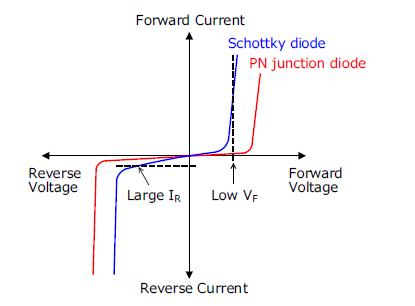
\includegraphics[width=0.5\textwidth]{tech/images/voltage-drop.png}
    \caption{Forward Voltage Drop in Different Diode Types}
    \label{fig:forward-voltage_drop}
    % Diagram showing the forward voltage drop across different types of diodes.
\end{figure}

\subsubsection*{Current Flow in a Diode}
As mentioned earlier, diodes allow current to flow in only one direction. This is due to the PN junction inside the diode, which creates a barrier that prevents current from flowing in the reverse direction. When you apply a forward voltage, this barrier is reduced, and current can flow. Think of it like a gate that only opens one way—pretty neat, right?

\begin{figure}[h]
    \centering
    \begin{circuitikz}
        % First circuit - Forward bias
        \draw (0,0) node[left] {+} 
            to[battery] (0,-2) node[left] {-};
        \draw (0,0) -- (2,0);
        \draw (2,-2) -- (0,-2);
        \draw (2,0) to[D] (2,-2);
        
        % Current flow arrow
        \draw[->, thick, blue] (1,0.3) -- (3,0.3) 
            node[midway, above] {Current flows};
        
        % Label
        \node[below] at (2,-2.5) {Forward Bias};

        % Second circuit - Reverse bias (shifted right)
        \begin{scope}[xshift=6cm]
            \draw (0,0) node[left] {-} 
                to[battery2] (0,-2) node[left] {+};
            \draw (0,0) -- (2,0);
            \draw (2,-2) -- (0,-2);
            \draw (2,0) to[D] (2,-2);
            
            % No current flow symbol (red X)
            \draw[red, thick] (1.7,0.2) -- (2.3,0.5);
            \draw[red, thick] (1.7,0.5) -- (2.3,0.2);
            \node[above] at (2,0.5) {No current};
            
            % Label
            \node[below] at (2,-2.5) {Reverse Bias};
        \end{scope}
    \end{circuitikz}
    \caption{Current Flow in a Diode: Forward bias allows current to flow (left), while reverse bias blocks current flow (right)}
    \label{fig:diode_current_flow}
\end{figure}

\subsubsection*{Cathode Marking on a Diode}
Ever wondered how to tell which side of a diode is the cathode? It's usually marked with a stripe on the package. This stripe is your guide to identifying the cathode, so you don't accidentally connect it the wrong way around. It's like the diode's way of saying, "Hey, this end goes here!"

\begin{figure}[th]
    \centering
    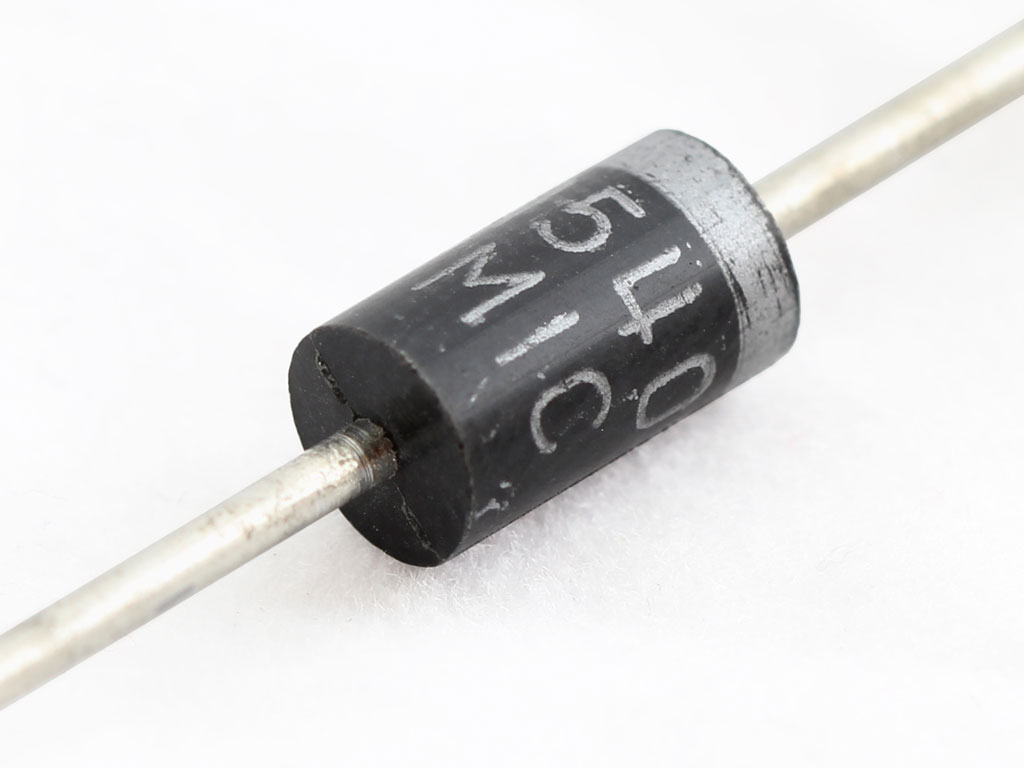
\includegraphics[width=0.3\textwidth]{tech/images/diode.jpeg}
    \caption{Cathode Marking on a Diode: The cathode end is typically identified by a stripe or band around the body of the diode. This marking is crucial for correct installation as diodes must be oriented properly to function. The stripe represents the 'bar' part of the diode symbol, making it easy to correlate the physical component with its schematic representation.}
    \label{fig:cathode_marking}
    % Image showing the marking of the cathode lead on a semiconductor diode.
\end{figure}

\subsubsection*{Light Emission in an LED}
Light-emitting diodes (LEDs) are a special type of diode that emit light when forward current is applied. This happens because the electrons recombine with holes in the semiconductor material, releasing energy in the form of photons. The color of the light depends on the energy gap of the semiconductor material. So, next time you see an LED light up, you'll know it's all about those electrons getting cozy with holes!

\begin{figure}[h]
    \centering
    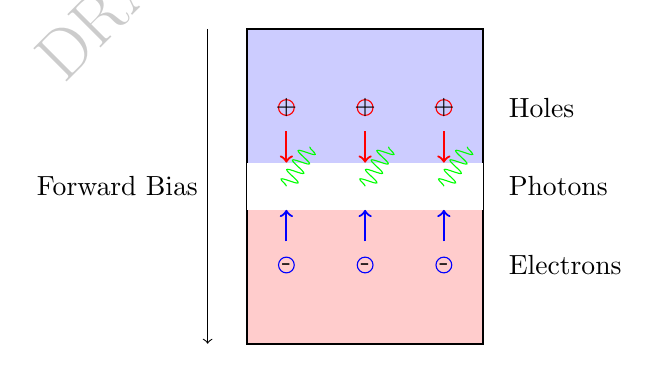
\begin{tikzpicture}
        % P-N Junction structure
        \fill[blue!20] (0,0) rectangle (3,2) node[pos=.5] {P-type};
        \fill[red!20] (0,-2) rectangle (3,0) node[pos=.5] {N-type};
        \draw[black, thick] (0,-2) rectangle (3,2);
        \draw[black, thick] (0,0) -- (3,0);
        
        % Depletion region
        \fill[white!20] (0,-0.3) rectangle (3,0.3);
        
        % Electrons and holes
        \foreach \x in {0.5,1.5,2.5} {
            % Electrons (negative charges)
            \draw[blue] (\x,-1) circle (0.1) node[black] {-};
            \draw[->, blue, thick] (\x,-0.7) -- (\x,-0.3);
            
            % Holes (positive charges)
            \draw[red] (\x,1) circle (0.1) node[black] {+};
            \draw[->, red, thick] (\x,0.7) -- (\x,0.3);
        }
        
        % Light emission
        \foreach \x in {0.5,1.5,2.5} {
            \draw[green, decorate, decoration={snake,amplitude=3pt,segment length=4pt}]
                (\x,0) -- (\x+0.3,0.5);
        }
        
        % Labels
        \node[right] at (3.2,1) {Holes};
        \node[right] at (3.2,-1) {Electrons};
        \node[right] at (3.2,0) {Photons};
        
        % Battery connection
        \draw[->] (-0.5,2) -- (-0.5,-2) node[midway, left] {Forward Bias};
        
    \end{tikzpicture}
    \caption{Light Emission in an LED: When electrons from the N-type material recombine with holes in the P-type material at the junction, energy is released as photons (light)}
    \label{fig:led_light_emission}
\end{figure}

\subsubsection*{Diode Electrodes}
Every diode has two electrodes: the anode and the cathode. The anode is the positive side, and the cathode is the negative side. When you apply a forward voltage, current flows from the anode to the cathode. It's like the diode's way of saying, "This is the way, folks!"

\begin{figure}[h]
    \centering
    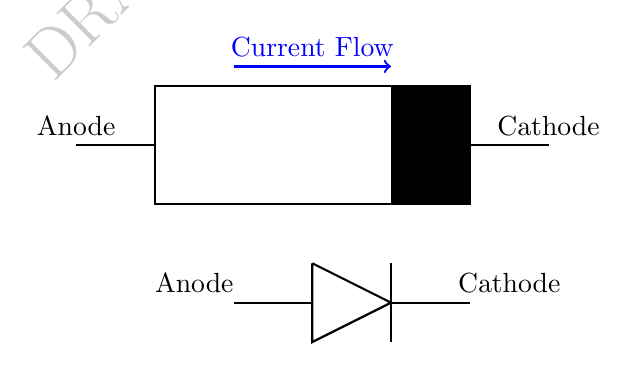
\begin{tikzpicture}
        % Main diode body
        \draw[thick] (0,0) rectangle (4,1.5);
        
        % Leads
        \draw[thick] (-1,0.75) -- (0,0.75);
        \draw[thick] (4,0.75) -- (5,0.75);
        
        % Cathode stripe
        \fill[black] (3,0) rectangle (4,1.5);
        
        % Labels
        \node[above] at (-1.0,0.75) {Anode};
        \node[above] at (5.0,0.75) {Cathode};
        
        % Circuit symbol below
        \begin{scope}[yshift=-2cm]
            \draw[thick] (1,0.75) -- (2,0.75);
            \draw[thick] (2,1.25) -- (2,0.25) -- (3,0.75) -- (2,1.25);
            \draw[thick] (3,1.25) -- (3,0.25);
            \draw[thick] (3,0.75) -- (4,0.75);
            
            % Labels for symbol
            \node[above] at (0.5,0.75) {Anode};
            \node[above] at (4.5,0.75) {Cathode};
        \end{scope}
        
        % Add direction arrow
        \draw[->, thick, blue] (1,1.75) -- (3,1.75) 
            node[midway, above] {Current Flow};
    \end{tikzpicture}
    \caption{Diode Electrodes: Physical package (top) showing the cathode stripe marking, and circuit symbol (bottom) with current flow direction}
    \label{fig:diode_electrodes}
\end{figure}

\begin{table}[h]
    \centering
    \caption{Comparison of Forward Voltage Drop in Diode Types}
    \label{tab:forward_voltage_comparison}
    \begin{tabular}{|l|c|}
        \hline
        \textbf{Diode Type} & \textbf{Forward Voltage Drop (V)} \\
        \hline
        Silicon Diode & 0.7 \\
        Schottky Diode & 0.3 \\
        Germanium Diode & 0.3 \\
        LED (Red) & 1.8 \\
        LED (Blue) & 3.3 \\
        \hline
    \end{tabular}
\end{table}

\subsubsection*{Questions}

\begin{tcolorbox}[colback=gray!10!white,colframe=black!75!black,title={T6B01}]
    Which is true about forward voltage drop in a diode?
    \begin{enumerate}[label=\Alph*),noitemsep]
        \item \textbf{It is lower in some diode types than in others}
        \item It is proportional to peak inverse voltage
        \item It indicates that the diode is defective
        \item It has no impact on the voltage delivered to the load
    \end{enumerate}
\end{tcolorbox}
The forward voltage drop varies depending on the diode type, as different materials and constructions lead to different energy barriers. This is why some diodes, like Schottky diodes, have a lower forward voltage drop compared to silicon diodes.

\begin{tcolorbox}[colback=gray!10!white,colframe=black!75!black,title={T6B02}]
    What electronic component allows current to flow in only one direction?
    \begin{enumerate}[label=\Alph*),noitemsep]
        \item Resistor
        \item Fuse
        \item \textbf{Diode}
        \item Driven element
    \end{enumerate}
\end{tcolorbox}
A diode is specifically designed to allow current to flow in only one direction, thanks to its PN junction.

\begin{tcolorbox}[colback=gray!10!white,colframe=black!75!black,title={T6B06}]
    How is the cathode lead of a semiconductor diode often marked on the package?
    \begin{enumerate}[label=\Alph*),noitemsep]
        \item With the word "cathode"
        \item \textbf{With a stripe}
        \item With the letter C
        \item With the letter K
    \end{enumerate}
\end{tcolorbox}
The cathode is typically marked with a stripe on the diode's package, making it easy to identify.

\begin{tcolorbox}[colback=gray!10!white,colframe=black!75!black,title={T6B07}]
    What causes a light-emitting diode (LED) to emit light?
    \begin{enumerate}[label=\Alph*),noitemsep]
        \item \textbf{Forward current}
        \item Reverse current
        \item Capacitively-coupled RF signal
        \item Inductively-coupled RF signal
    \end{enumerate}
\end{tcolorbox}
When forward current is applied to an LED, electrons recombine with holes, releasing energy in the form of photons, which we see as light.

\begin{tcolorbox}[colback=gray!10!white,colframe=black!75!black,title={T6B09}]
    What are the names for the electrodes of a diode?
    \begin{enumerate}[label=\Alph*),noitemsep]
        \item Plus and minus
        \item Source and drain
        \item \textbf{Anode and cathode}
        \item Gate and base
    \end{enumerate}
\end{tcolorbox}
The two electrodes of a diode are called the anode (positive side) and the cathode (negative side). These terms are standard in diode terminology.

\subsection{Transistors (BJT, FET), Amplification}
\label{subsec:transistors}

Transistors are semiconductor devices that serve as the fundamental building blocks of modern electronics. Think of them as tiny electronic switches or amplifiers that can control the flow of electricity. What makes transistors truly remarkable is that they can use a small electrical signal to control a much larger one—like using a small stream of water to control a powerful river!

At their core, transistors are made from layers of semiconductor materials (usually silicon) that have been specially treated or "doped" to create specific electrical properties. These layers work together to control the flow of electrons in ways that make our modern electronic devices possible. Without transistors, we wouldn't have computers, smartphones, or any of the digital technology we rely on today.

Transistors can perform three essential functions:
\begin{itemize}
    \item Amplification: Making weak signals stronger
    \item Switching: Turning electrical signals on and off
    \item Control: Regulating the amount of current flowing through a circuit
\end{itemize}

In this section, we'll explore how transistors work, focusing on two main types: Bipolar Junction Transistors (BJTs) and Field-Effect Transistors (FETs). We'll also dive into the concept of amplification and how these little devices can make weak signals strong enough to be useful.

\subsubsection*{Transistor as an Electronic Switch}
One of the most common uses of a transistor is as an electronic switch. Imagine you have a light bulb, and you want to turn it on and off using a small signal. A transistor can do this job perfectly. When a small current or voltage is applied to the base (in a BJT) or the gate (in a FET), it allows a larger current to flow between the collector and emitter (in a BJT) or the drain and source (in a FET). This is like flipping a switch—except it’s all done electronically, no physical flipping required!



\subsubsection*{Structure of a Transistor}
A transistor, whether it's a BJT or a FET, is made up of three regions of semiconductor material, each connected to an electrode (an electrical conductor through which current can flow into or out of a component). In a BJT, these electrodes are called the emitter, base, and collector. The base is the middle layer, and it's very thin. The emitter and collector are on either side. In a FET, the electrodes are called the source, gate, and drain. The gate controls the flow of electrons from the source to the drain. Think of it like a water faucet: the gate is the handle, and the source and drain are the pipes.

% Illustration of the three regions of a bipolar junction transistor.
\begin{figure}[h!]
    \centering
    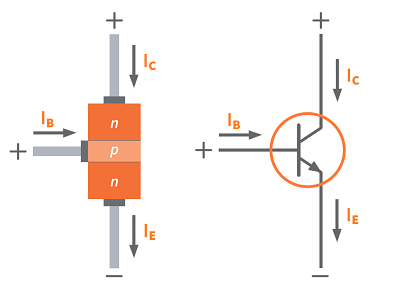
\includegraphics[width=0.6\textwidth]{tech/images/bjt-transistor.png}
    \caption{Bipolar Junction Transistor Structure: Cross-sectional view of an NPN transistor showing the three semiconductor layers (Emitter, Base, and Collector), along with the symbol. The base region is very thin compared to the emitter and collector regions. Electron flow  $I_c$, $I_b$, $I_e$ represent the current on the collector, base, and emitter, respectively. }
    \label{fig:bjt_structure}
\end{figure}

\subsubsection*{Field-Effect Transistor (FET)}
FETs are a bit different from BJTs. Instead of using a current to control the flow of electrons, FETs use a voltage. The gate in a FET is like a gatekeeper—it controls how many electrons can pass from the source to the drain. FETs are often used in low-power applications because they’re very efficient. They’re also the backbone of modern integrated circuits, like the ones in your smartphone.

% % Diagram of a Field-Effect Transistor (FET) showing the gate, drain, and source.
% \begin{figure}[h!]
%     \centering
%     % \includegraphics[width=0.6\textwidth]{fet_structure.svg}
%     \caption{Field-Effect Transistor (FET) Structure. The diagram shows the gate, drain, and source regions.}
%     \label{fig:fet_structure}
% \end{figure}

\subsubsection*{What Does FET Stand For?}
FET stands for Field-Effect Transistor. The “field-effect” part refers to the way the gate controls the flow of electrons. It creates an electric field that either allows or blocks the flow of electrons from the source to the drain. This is different from a BJT, which uses a current to control the flow.

\subsubsection*{Power Gain and Amplification}
One of the most important features of a transistor is its ability to amplify signals. This means it can take a small input signal and produce a larger output signal. The amount of amplification is called the gain. For example, if you have a weak radio signal, a transistor can amplify it so that it’s strong enough to drive a speaker. This is why transistors are used in everything from radios to amplifiers.

% Graph showing the power gain provided by a transistor.
\begin{figure}[h!]
    \centering
    \begin{minipage}{0.45\textwidth}
        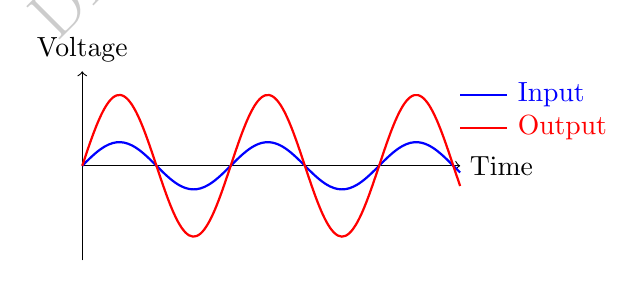
\begin{tikzpicture}[scale=0.6]
            % Grid and axes
            \draw[->] (0,0) -- (8,0) node[right] {Time};
            \draw[->] (0,-2) -- (0,2) node[above] {Voltage};
            
            % Input signal (smaller amplitude)
            \draw[blue, thick, smooth] plot[domain=0:8,samples=100] 
                (\x,{0.5*sin(2*\x r)});
                
            % Output signal (larger amplitude)
            \draw[red, thick, smooth] plot[domain=0:8,samples=100] 
                (\x,{1.5*sin(2*\x r)});
            
            \draw[blue, thick, smooth] (8,1.5) -- (9,1.5) node[right]{Input};
            \draw[red, thick, smooth] (8,0.8) -- (9,0.8) node[right]{Output};
        \end{tikzpicture}
        \caption*{(a) Signal amplification: A small input signal (blue) is amplified to produce a larger output signal (red)}
    \end{minipage}%
    \hfill%
    \begin{minipage}{0.4\textwidth}
        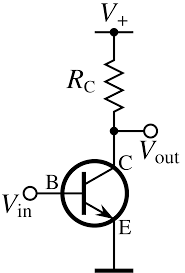
\includegraphics[width=0.3\textwidth]{tech/images/transistor-amplifier.png}
        \caption*{(b) Schematic diagram of a common emitter amplifier circuit}
    \end{minipage}
    \caption{Transistor Power Gain. }
    \label{fig:transistor_power_gain}
\end{figure}

\subsubsection*{Gain: The Measure of Amplification}
Gain is a term that describes how much a device can amplify a signal. It’s usually expressed as a ratio of the output signal to the input signal. For example, if the output signal is 10 times stronger than the input signal, the gain is 10. Gain is a crucial parameter in designing circuits, especially in audio amplifiers and radio receivers.

\subsubsection*{Electrodes of a Bipolar Junction Transistor}
In a BJT, the three electrodes are called the emitter, base, and collector. The emitter is where the electrons start their journey, the base controls the flow, and the collector is where they end up. It’s like a relay race: the emitter hands off the electrons to the base, which then passes them to the collector.

% Diagram labeling the emitter, base, and collector of a bipolar junction transistor.
% \begin{figure}[h!]
%     \centering
%     % \includegraphics[width=0.6\textwidth]{bjt_electrodes.svg}
%     \caption{BJT Electrodes. The diagram labels the emitter, base, and collector of a BJT.}
%     \label{fig:bjt_electrodes}
% \end{figure}

\subsubsection*{Comparison of BJT and FET Transistors}
To wrap things up, let’s compare BJTs and FETs. BJTs are current-controlled devices, while FETs are voltage-controlled. BJTs are generally better for high-power applications, while FETs are more efficient for low-power applications. Both have their strengths and weaknesses, and the choice between them depends on the specific application.

\begin{table}[h!]
    \centering
    \begin{tabular}{|l|l|l|}
        \hline
        \textbf{Characteristic} & \textbf{BJT} & \textbf{FET} \\
        \hline
        Control Mechanism & Current & Voltage \\
        Power Efficiency & Lower & Higher \\
        Input Impedance & Low & High \\
        Typical Use & High-power & Low-power \\
        \hline
    \end{tabular}
    \caption{Comparison of BJT and FET Transistors.}
    \label{tab:bjt_fet_comparison}
\end{table}

\subsubsection*{Questions}
\begin{tcolorbox}[colback=gray!10!white,colframe=black!75!black,title={T6B03}]
    Which of these components can be used as an electronic switch?
    \begin{enumerate}[label=\Alph*),noitemsep]
        \item Varistor
        \item Potentiometer
        \item \textbf{Transistor}
        \item Thermistor
    \end{enumerate}
\end{tcolorbox}
A transistor can be used as an electronic switch because it can control the flow of current between two terminals using a small input signal. Varistors, potentiometers, and thermistors do not have this capability.

\begin{tcolorbox}[colback=gray!10!white,colframe=black!75!black,title={T6B04}]
    Which of the following components can consist of three regions of semiconductor material?
    \begin{enumerate}[label=\Alph*),noitemsep]
        \item Alternator
        \item \textbf{Transistor}
        \item Triode
        \item Pentagrid converter
    \end{enumerate}
\end{tcolorbox}
A transistor consists of three regions of semiconductor material: the emitter, base, and collector in a BJT, or the source, gate, and drain in a FET. Alternators, triodes, and pentagrid converters do not have this structure.

\begin{tcolorbox}[colback=gray!10!white,colframe=black!75!black,title={T6B05}]
    What type of transistor has a gate, drain, and source?
    \begin{enumerate}[label=\Alph*),noitemsep]
        \item Varistor
        \item \textbf{Field-effect}
        \item Tesla-effect
        \item Bipolar junction
    \end{enumerate}
\end{tcolorbox}
A Field-Effect Transistor (FET) has a gate, drain, and source. These are the three terminals that control the flow of electrons in a FET. Varistors and BJTs do not have these terminals.

\begin{tcolorbox}[colback=gray!10!white,colframe=black!75!black,title={T6B08}]
    What does the abbreviation FET stand for?
    \begin{enumerate}[label=\Alph*),noitemsep]
        \item Frequency Emission Transmitter
        \item Fast Electron Transistor
        \item Free Electron Transmitter
        \item \textbf{Field Effect Transistor}
    \end{enumerate}
\end{tcolorbox}
FET stands for Field-Effect Transistor. It refers to the way the gate controls the flow of electrons using an electric field.

\begin{tcolorbox}[colback=gray!10!white,colframe=black!75!black,title={T6B10}]
    Which of the following can provide power gain?
    \begin{enumerate}[label=\Alph*),noitemsep]
        \item Transformer
        \item \textbf{Transistor}
        \item Reactor
        \item Resistor
    \end{enumerate}
\end{tcolorbox}
A transistor can provide power gain by amplifying a small input signal to produce a larger output signal. Transformers, reactors, and resistors do not have this capability.

\begin{tcolorbox}[colback=gray!10!white,colframe=black!75!black,title={T6B11}]
    What is the term that describes a device's ability to amplify a signal?
    \begin{enumerate}[label=\Alph*),noitemsep]
        \item \textbf{Gain}
        \item Forward resistance
        \item Forward voltage drop
        \item On resistance
    \end{enumerate}
\end{tcolorbox}
Gain is the term that describes a device's ability to amplify a signal. It is the ratio of the output signal to the input signal.

\begin{tcolorbox}[colback=gray!10!white,colframe=black!75!black,title={T6B12}]
    What are the names of the electrodes of a bipolar junction transistor?
    \begin{enumerate}[label=\Alph*),noitemsep]
        \item Signal, bias, power
        \item \textbf{Emitter, base, collector}
        \item Input, output, supply
        \item Pole one, pole two, output
    \end{enumerate}
\end{tcolorbox}
The electrodes of a bipolar junction transistor are called the emitter, base, and collector. These are the three terminals that control the flow of current in a BJT.

\section{Circuit Symbols and Schematics}
\subsection{Reading Schematics}
\label{subsec:schem-reading}

When you first look at a schematic diagram, it might seem like a jumble of lines and symbols. But don't worry, it's not as complicated as it looks! A schematic is essentially a map of an electrical circuit, showing how components are connected together. It uses standardized symbols to represent different components, making it easier for engineers and hobbyists to understand and build circuits without needing to know what each component looks like physically.

\subsubsection*{The Purpose of Schematics}
The primary purpose of a schematic is to provide a clear and concise representation of an electrical circuit. Unlike a physical layout, which shows where components are placed on a board, a schematic focuses on the connections between components. This allows you to understand how the circuit functions without getting bogged down by the physical arrangement.

\subsubsection*{Standard Symbols in Schematics}
In schematics, each component is represented by a unique symbol. For example, a resistor is typically shown as a zigzag line, while a transistor might be represented by a combination of lines and arrows. Batteries are often depicted as a series of long and short lines, and the ground symbol is usually a horizontal line with three downward-pointing lines. These symbols are standardized, so once you learn them, you can read any schematic.

\subsubsection*{Identifying Components}
Let's take a closer look at some common components and their symbols:

\begin{itemize}[noitemsep]    \item \textbf{Resistor}: Represented by a zigzag line. Resistors are used to limit the flow of current in a circuit.
    \item \textbf{Transistor}: Typically shown as a combination of lines and arrows. Transistors are used to amplify or switch electronic signals.
    \item \textbf{Battery}: Depicted as a series of long and short lines. Batteries provide the power needed to run the circuit.
    \item \textbf{Ground Symbol}: A horizontal line with three downward-pointing lines. This symbol represents the reference point in a circuit, often connected to the earth or a common return path.
\end{itemize}

\subsubsection*{Capacitors and Inductors}
Capacitors and inductors are also common in electronic circuits. Capacitors, represented by two parallel lines, store electrical energy, while inductors, shown as a series of loops, store energy in a magnetic field. Both components are crucial for filtering and tuning circuits.

\subsubsection*{Light-Emitting Diodes (LEDs)}
LEDs are represented by a triangle with a line pointing away from it, often with a small arrow indicating the direction of light emission. LEDs are used to indicate the status of a circuit or to provide illumination.

\subsubsection*{Variable Components}
Variable components, like resistors and inductors, are represented with an arrow through their standard symbols. These components allow you to adjust the resistance or inductance in a circuit, making them useful for tuning and calibration.

\subsubsection*{Transformers}
Transformers are depicted as two coils with a line between them. They are used to step up or step down voltage levels in a circuit, making them essential for power supply designs.

\subsubsection*{Antennas}
Antennas are represented by a simple line with a small triangle at the end. They are used to transmit or receive radio signals, making them a key component in radio circuits.

% \begin{figure}[h]
%     \centering
%     %\includegraphics[width=0.8\textwidth]{schematic-example}
%     \caption{Example schematic diagram with standard electronic components.}
%     \label{fig:schematic-example}
%     % Prompt: A detailed schematic diagram showing common electronic components like resistors, capacitors, transistors, and LEDs.
% \end{figure}

% \begin{figure}[h]
%     \centering
%     %\includegraphics[width=0.8\textwidth]{component-symbols}
%     \caption{Comparison of physical components and their schematic symbols.}
%     \label{fig:component-symbols}
%     % Prompt: A comparison of physical components and their schematic symbols.
% \end{figure}

\begin{table}[h]
    \centering
    \begin{tabular}{|c|c|c|c|}
        \hline
        \begin{tikzpicture}[baseline]
            \draw (0,0) to[R] (1,0);
        \end{tikzpicture} &
        \begin{tikzpicture}[baseline]
            \draw (0,0) to[pR,scale=0.7] (1,0);
        \end{tikzpicture} &
        \begin{tikzpicture}[baseline]
            \draw (0,0) to[C] (1,0);
        \end{tikzpicture} &
        \begin{tikzpicture}[baseline]
            \draw (0,0) to[vC] (1,0);
        \end{tikzpicture} \\[1ex]
        Resistor & Variable Resistor & Capacitor & Variable Capacitor \\[3ex]
        \hline
        \begin{tikzpicture}[baseline]
            \draw (0,0) to[L] (1,0);
        \end{tikzpicture} &
        \begin{tikzpicture}[baseline]
            \draw (0,0) to[vL] (1,0);
        \end{tikzpicture} &
        \begin{tikzpicture}[baseline]
            \draw (0,0) node[transformer core,scale=0.7]{};
        \end{tikzpicture} &
        \begin{tikzpicture}[baseline=-1.5ex]
            \draw (0,-1) node[antenna,scale=0.7] {};
        \end{tikzpicture} \\[1ex]
        Inductor & Variable Inductor & Transformer & Antenna \\[3ex]
        \hline
        \begin{tikzpicture}[baseline]
            \draw (0,0) to[D,scale=0.7] (1,0);
        \end{tikzpicture} &
        \begin{tikzpicture}[baseline]
            \draw (0,0) to[led,scale=0.7] (1,0);
        \end{tikzpicture} &
        \begin{tikzpicture}[baseline]
            \draw (0,0) to[zD,scale=0.7] (1,0);
        \end{tikzpicture} &
        \begin{tikzpicture}[baseline]
            \draw (0,0) to[bulb] (1,0);
        \end{tikzpicture} \\[1ex]
        Diode & LED & Zener Diode & Bulb \\[3ex]
        \hline
        \begin{tikzpicture}[baseline]
            \draw (0,0) node[npn,scale=0.7] (npn) {};
        \end{tikzpicture} &
        \begin{tikzpicture}[baseline]
            \draw (0,0) node[pnp,scale=0.7] (pnp) {};
        \end{tikzpicture} &
        \begin{tikzpicture}[baseline]
            \draw (0,0) to[battery1] (1,0);
        \end{tikzpicture} &
        \begin{tikzpicture}[baseline]
            \draw (0,0) node[ground] {};
        \end{tikzpicture} \\[1ex]
        Transistor (NPN) & Transistor (PNP) & Battery & Ground \\[3ex]
        \hline
    \end{tabular}
    \caption{Common electronic components and their schematic symbols.}
    \label{tab:component-symbols}
\end{table}

\subsubsection*{Questions}

\begin{tcolorbox}[colback=gray!10!white,colframe=black!75!black,title={T6C01}]
    What is the name of an electrical wiring diagram that uses standard component symbols?
    \begin{enumerate}[label=\Alph*),noitemsep]
        \item Bill of materials
        \item Connector pinout
        \item \textbf{Schematic}
        \item Flow chart
    \end{enumerate}
\end{tcolorbox}
A schematic is the correct term for an electrical wiring diagram that uses standard component symbols. The other options refer to different types of documentation.



\begin{tcolorbox}[
    colback=gray!10!white,
    colframe=black!75!black,
    title={T6C02},
    sidebyside,
    sidebyside align=top,
    lefthand width=0.45\textwidth
]
What is component 1 in figure T-1?
\begin{enumerate}[label=\Alph*),noitemsep]
    \item \textbf{Resistor}
    \item Transistor
    \item Battery
    \item Connector
\end{enumerate}
\tcblower
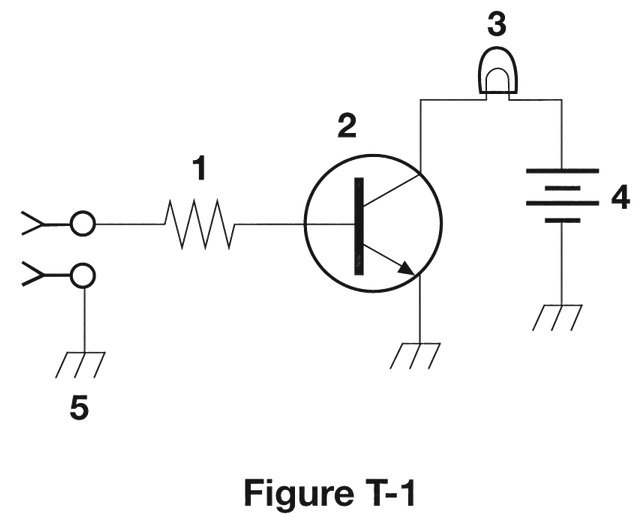
\includegraphics[width=0.7\textwidth]{tech/images/t1.png}
\end{tcolorbox}
Component 1 in figure T-1 is a resistor. Resistors are commonly represented by a zigzag line in schematics.

\begin{tcolorbox}[
    colback=gray!10!white,
    colframe=black!75!black,
    title={T6C03},
    sidebyside,
    sidebyside align=top,
    lefthand width=0.45\textwidth
]
What is component 2 in figure T-1?
\begin{enumerate}[label=\Alph*),noitemsep]
    \item Resistor
    \item \textbf{Transistor}
    \item Indicator lamp
    \item Connector
\end{enumerate}
\tcblower
\includegraphics[width=0.7\textwidth]{tech/images/t1.png}
\end{tcolorbox}
Component 2 in figure T-1 is a transistor. Transistors are typically represented by a combination of lines and arrows.

\begin{tcolorbox}[
    colback=gray!10!white,
    colframe=black!75!black,
    title={T6C04},
    sidebyside,
    sidebyside align=top,
    lefthand width=0.45\textwidth
]
What is component 3 in figure T-1?
\begin{enumerate}[label=\Alph*),noitemsep]
    \item Resistor
    \item Transistor
    \item \textbf{Lamp}
    \item Ground symbol
\end{enumerate}
\tcblower
\includegraphics[width=0.7\textwidth]{tech/images/t1.png}
\end{tcolorbox}
Component 3 in figure T-1 is a lamp. Lamps are often represented by a circle with a cross inside.

\begin{tcolorbox}[
    colback=gray!10!white,
    colframe=black!75!black,
    title={T6C05},
    sidebyside,
    sidebyside align=top,
    lefthand width=0.45\textwidth
]
What is component 4 in figure T-1?
\begin{enumerate}[label=\Alph*),noitemsep]
    \item Resistor
    \item Transistor
    \item Ground symbol
    \item \textbf{Battery}
\end{enumerate}
\tcblower
\includegraphics[width=0.7\textwidth]{tech/images/t1.png}
\end{tcolorbox}
Component 4 in figure T-1 is a battery. Batteries are typically represented by a series of long and short lines.



\begin{tcolorbox}[
    colback=gray!10!white,
    colframe=black!75!black,
    title={T6C06},
    sidebyside,
    sidebyside align=top,
    lefthand width=0.45\textwidth
]
What is component 6 in figure T-2?
\begin{enumerate}[label=\Alph*),noitemsep]
    \item Resistor
    \item \textbf{Capacitor}
    \item Regulator IC
    \item Transistor
\end{enumerate}
\tcblower
\includegraphics[width=0.7\textwidth]{tech/images/t2.png}
\end{tcolorbox}
Component 6 in figure T-2 is a capacitor. Capacitors are represented by two parallel lines in schematics.

\begin{tcolorbox}[
    colback=gray!10!white,
    colframe=black!75!black,
    title={T6C07},
    sidebyside,
    sidebyside align=top,
    lefthand width=0.45\textwidth
]
What is component 8 in figure T-2?
\begin{enumerate}[label=\Alph*),noitemsep]
    \item Resistor
    \item Inductor
    \item Regulator IC
    \item \textbf{Light emitting diode}
\end{enumerate}
\tcblower
\includegraphics[width=0.7\textwidth]{tech/images/t2.png}
\end{tcolorbox}
Component 8 in figure T-2 is a light-emitting diode (LED). LEDs are represented by a triangle with a line and arrow.

\begin{tcolorbox}[
    colback=gray!10!white,
    colframe=black!75!black,
    title={T6C08},
    sidebyside,
    sidebyside align=top,
    lefthand width=0.45\textwidth
]
What is component 9 in figure T-2?
\begin{enumerate}[label=\Alph*),noitemsep]
    \item Variable capacitor
    \item Variable inductor
    \item \textbf{Variable resistor}
    \item Variable transformer
\end{enumerate}
\tcblower
\includegraphics[width=0.7\textwidth]{tech/images/t2.png}
\end{tcolorbox}
Component 9 in figure T-2 is a variable resistor. Variable resistors are represented by a zigzag line with an arrow.

\begin{tcolorbox}[
    colback=gray!10!white,
    colframe=black!75!black,
    title={T6C09},
    sidebyside,
    sidebyside align=top,
    lefthand width=0.45\textwidth
]
What is component 4 in figure T-2?
\begin{enumerate}[label=\Alph*),noitemsep]
    \item Variable inductor
    \item Double-pole switch
    \item Potentiometer
    \item \textbf{Transformer}
\end{enumerate}
\tcblower
\includegraphics[width=0.7\textwidth]{tech/images/t2.png}
\end{tcolorbox}
Component 4 in figure T-2 is a transformer. Transformers are represented by two coils with a line between them.

\begin{tcolorbox}[
    colback=gray!10!white,
    colframe=black!75!black,
    title={T6C10},
    sidebyside,
    sidebyside align=top,
    lefthand width=0.45\textwidth
]
What is component 3 in figure T-3?
\begin{enumerate}[label=\Alph*),noitemsep]
    \item Connector
    \item Meter
    \item Variable capacitor
    \item \textbf{Variable inductor}
\end{enumerate}
\tcblower
\includegraphics[width=0.7\textwidth]{tech/images/t3.png}
\end{tcolorbox}
Component 3 in figure T-3 is a variable inductor. Variable inductors are represented by a series of loops with an arrow.

\begin{tcolorbox}[
    colback=gray!10!white,
    colframe=black!75!black,
    title={T6C11},
    sidebyside,
    sidebyside align=top,
    lefthand width=0.45\textwidth
]
What is component 4 in figure T-3?
\begin{enumerate}[label=\Alph*),noitemsep]
    \item \textbf{Antenna}
    \item Transmitter
    \item Dummy load
    \item Ground
\end{enumerate}
\tcblower
\includegraphics[width=0.7\textwidth]{tech/images/t3.png}
\end{tcolorbox}
Component 4 in figure T-3 is an antenna. Antennas are represented by a line with a small triangle at the end.

\begin{tcolorbox}[colback=gray!10!white,colframe=black!75!black,title={T6C12}]
    Which of the following is accurately represented in electrical schematics?
    \begin{enumerate}[label=\Alph*),noitemsep]
        \item Wire lengths
        \item Physical appearance of components
        \item \textbf{Component connections}
        \item All these choices are correct
    \end{enumerate}
\end{tcolorbox}
Component connections are accurately represented in electrical schematics. Wire lengths and physical appearances are not typically shown in schematics.

\section{Integrated Circuits, Filters, Rectifiers}
\subsection{Rectifiers, Regulators, etc.}
\label{subsec:rect-reg}

\subsubsection*{Rectifiers: Turning AC into DC}
Let's start with rectifiers, the power behind the throne of the electronics world. A rectifier is a device that converts alternating current (AC) into direct current (DC). Think of it as a traffic cop for electrons, only letting them flow in one direction. This is crucial because many electronic devices, like your smartphone or laptop, need DC to function properly. The rectifier achieves this by using diodes, which act like one-way valves for electrical current. 

For example, in a simple half-wave rectifier, only the positive half of the AC waveform is allowed through, while the negative half is blocked. A full-wave rectifier, on the other hand, flips the negative half of the waveform to make it positive, resulting in a smoother DC output. You can see this process illustrated in Figure~\ref{fig:rectifier}.

\begin{figure}[h]
    \centering
    \footnotesize
    \begin{minipage}{0.4\textwidth}
        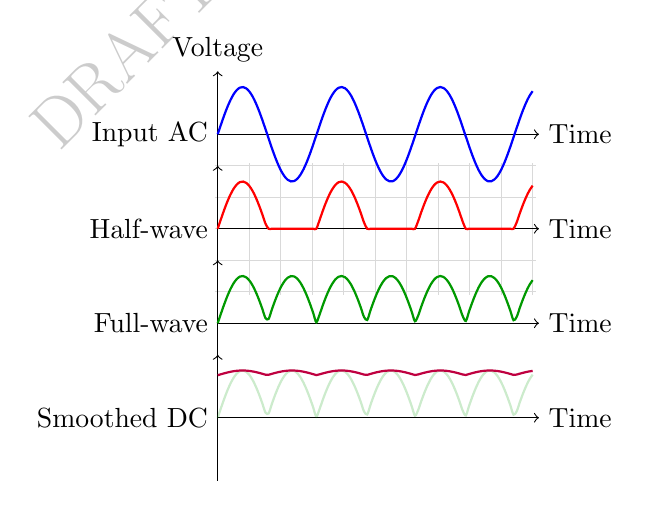
\begin{tikzpicture}[scale=0.4]
            % Grid for all plots
            \draw[gray!30, step=1] (-0.1,-2.1) grid (10.1,2.1);
            
            % Input AC Signal
            \begin{scope}[yshift=3cm]
                \draw[->] (0,0) -- (10.2,0) node[right] {Time};
                \draw[->] (0,-2) -- (0,2) node[above] {Voltage};
                \draw[blue, thick, smooth] plot[domain=0:10,samples=100] 
                    (\x,{1.5*sin(2*\x r)});
                \node[left] at (0,0) {Input AC};
            \end{scope}
            
            % Half-wave rectified
            \begin{scope}[yshift=0cm]
                \draw[->] (0,0) -- (10.2,0) node[right] {Time};
                \draw[->] (0,-2) -- (0,2) node[above] {};
                \draw[red, thick, smooth] plot[domain=0:10,samples=100] 
                    (\x,{max(0,1.5*sin(2*\x r))});
                \node[left] at (0,0) {Half-wave};
            \end{scope}
            
            % Full-wave rectified
            \begin{scope}[yshift=-3cm]
                \draw[->] (0,0) -- (10.2,0) node[right] {Time};
                \draw[->] (0,-2) -- (0,2) node[above] {};
                \draw[green!60!black, thick, smooth] plot[domain=0:10,samples=100] 
                    (\x,{abs(1.5*sin(2*\x r))});
                \node[left] at (0,0) {Full-wave};
            \end{scope}
            
            % Smoothed DC (with capacitor)
            \begin{scope}[yshift=-6cm]
                \draw[->] (0,0) -- (10.2,0) node[right] {Time};
                \draw[->] (0,-2) -- (0,2) node[above] {};
                % Base full-wave rectified
                \draw[green!60!black, thick, smooth, opacity=0.2] plot[domain=0:10,samples=100] 
                    (\x,{abs(1.5*sin(2*\x r))});
                % Smoothed output
                \draw[purple, thick, smooth] plot[domain=0:10,samples=100] 
                    (\x,{1.35+0.15*abs(sin(2*\x r))});
                \node[left] at (0,0) {Smoothed DC};
            \end{scope}
        \end{tikzpicture}
        \caption*{(a) Waveforms showing AC to DC conversion process}
    \end{minipage}%
    \hfill%
    \begin{minipage}{0.4\textwidth}
        \begin{circuitikz}[scale=0.4],american]
            % AC source
            \draw (0,5) to[sinusoidal voltage source, l_=AC] (0,-5);
        
            \draw (0,-5) -- (6,-5) -- (6, -4);
            \draw (0,5) -- (6,5) -- (6,4);
            \draw[->] (2,0) -- (1,0) -- (1,-6) --(12,-6)node[right]{$-$};
            \draw[->] (10,0) -- (12,0)node[right]{$+$};
            
            \draw (2,0)  to[D, -] (6,-4);
            \draw (6,-4)  to[D, -] (10,0);
            \draw (2,0)   to[D, -] (6,4);
            \draw (6,4)  to[D, -] (10,0);
             \draw[<->,dashed] (12,-6) -- (12,0) node[midway,above] {DC}; 
        \end{circuitikz}
        
        \caption*{(b) Four-diode bridge rectifier circuit}
    \end{minipage}
    \caption{AC to DC conversion using rectifiers. (a) Shows the progression from AC input to smoothed DC output: original AC signal, half-wave rectification, full-wave rectification, and smoothed DC after filtering. (b) Shows a typical bridge rectifier circuit that performs full-wave rectification using four diodes.}
    \label{fig:rectifier}
\end{figure}
    
\begin{table}[h]
    \centering
    \caption{Comparison of rectifier types.}
    \label{tab:rectifiers}
    \begin{tabular}{|l|l|l|}
    \hline
    \textbf{Type} & \textbf{Efficiency} & \textbf{Output} \\
    \hline
    Half-wave & Low & Pulsating DC \\
    Full-wave & Higher & Smoother DC \\
    Bridge & Highest & Smoother DC \\
    \hline
    \end{tabular}
\end{table}
    



\subsubsection*{Relays: The Electrically-Controlled Switch}
Next up, we have relays. A relay is essentially an electrically-controlled switch. When you send a small current through the relay's coil, it creates a magnetic field that pulls a switch to connect or disconnect a larger current. This is super handy when you want to control a high-power circuit with a low-power signal, like turning on a motor with a tiny button. 

% add a figure of a relay
\begin{figure}[h]
    \centering
    \begin{minipage}{0.24\textwidth}
        \includegraphics[width=\textwidth]{tech/images/relay.jpg}
        \caption*{(a) Relay}
    \end{minipage}%
    \hfill%
    \begin{minipage}{0.24\textwidth}
        \includegraphics[width=\textwidth]{tech/images/transformer.jpg}
        \caption*{(b) Transformer}
    \end{minipage}%
    \hfill%
    \begin{minipage}{0.24\textwidth}
        \centering
        \includegraphics[width=0.5\textwidth]{tech/images/multimeter.jpg}
        \caption*{(c) Multimeter}
    \end{minipage}%
    \hfill%
    \begin{minipage}{0.24\textwidth}
        \includegraphics[width=\textwidth]{tech/images/regulator.jpg}
        \caption*{(d) Voltage Regulator}
    \end{minipage}
    \caption{Common electronic components: (a) A relay for switching high-power circuits with low-power signals, (b) A transformer for changing AC voltage levels, (c) A multimeter for measuring electrical quantities, and (d) A voltage regulator for maintaining constant output voltage.}
    \label{fig:electronic-components}
\end{figure}


\subsubsection*{Shielded Wire: Keeping Signals Clean}
Ever wonder why some wires are wrapped in a metallic braid? That's shielded wire, and its job is to prevent unwanted signal coupling. In other words, it keeps your signals from getting mixed up with other signals nearby. This is especially important in radio circuits, where even a tiny bit of interference can mess things up. 

\subsubsection*{Meters: The Numeric Display of Electrical Quantities}
Meters are the gadgets that give you a numeric readout of electrical quantities like voltage, current, or resistance. They’re like the speedometer in your car, but for electricity. Whether it's an analog needle or a digital display, meters help you keep track of what's going on in your circuit.

\subsubsection*{Regulators: Keeping Voltage in Check}
A voltage regulator is like a thermostat for your power supply. It maintains a constant output voltage even when the input voltage or load current changes. Inside a typical linear regulator, a feedback circuit continuously monitors the output voltage and adjusts a control element (usually a transistor) to maintain the desired voltage level. For example, if the output voltage starts to drop due to increased load, the regulator compensates by allowing more current to flow through. Common regulators like the 7805 can take a varying input of 7-35V and provide a steady 5V output, perfect for powering digital circuits.

\subsubsection*{Transformers: Changing AC Voltage Levels}
Transformers are the workhorses of AC circuits. They can step up (increase) or step down (decrease) AC voltage levels. This is done using two coils of wire wrapped around a common core. When AC flows through the primary coil, it creates a magnetic field that induces a voltage in the secondary coil. The ratio of the number of turns in the coils determines the voltage change. For example, if you need to step down 120 V AC to 12 V AC, a transformer is your go-to device.

\subsubsection*{LEDs: The Visual Indicators}
Finally, let's talk about LEDs, or Light Emitting Diodes. These little guys are everywhere, from your TV remote to the indicator lights on your stereo. LEDs are great because they’re energy-efficient, long-lasting, and come in a variety of colors. They’re the perfect way to give you a visual cue about what’s happening in your circuit.



% \begin{figure}[h]
% \centering
% % \includegraphics{relay.svg} % Placeholder for the relay schematic
% \caption{Relay circuit schematic.}
% \label{fig:relay}
% % Prompt: Schematic of a relay circuit.
% \end{figure}

% \begin{figure}[h]
% \centering
% % \includegraphics{shielded-wire.svg} % Placeholder for the shielded wire illustration
% \caption{Shielded wire preventing signal interference.}
% \label{fig:shielded-wire}
% % Prompt: Illustration of shielded wire preventing signal interference.
% \end{figure}

\subsubsection*{Questions}

\begin{tcolorbox}[colback=gray!10!white,colframe=black!75!black,title={T6D01}]
Which of the following devices or circuits changes an alternating current into a varying direct current signal?
\begin{enumerate}[label=\Alph*),noitemsep]
    \item Transformer
    \item \textbf{Rectifier}
    \item Amplifier
    \item Reflector
\end{enumerate}
\end{tcolorbox}
A rectifier is specifically designed to convert AC to DC. Transformers change voltage levels, amplifiers increase signal strength, and reflectors are used in antennas, not for current conversion.

\begin{tcolorbox}[colback=gray!10!white,colframe=black!75!black,title={T6D02}]
What is a relay?
\begin{enumerate}[label=\Alph*),noitemsep]
    \item \textbf{An electrically-controlled switch}
    \item A current controlled amplifier
    \item An inverting amplifier
    \item A pass transistor
\end{enumerate}
\end{tcolorbox}
A relay uses a small electrical current to control a larger one, acting as a switch. The other options describe different types of amplifiers or transistors, not relays.

\begin{tcolorbox}[colback=gray!10!white,colframe=black!75!black,title={T6D03}]
Which of the following is a reason to use shielded wire?
\begin{enumerate}[label=\Alph*),noitemsep]
    \item To decrease the resistance of DC power connections
    \item To increase the current carrying capability of the wire
    \item \textbf{To prevent coupling of unwanted signals to or from the wire}
    \item To couple the wire to other signals
\end{enumerate}
\end{tcolorbox}
Shielded wire is used to prevent interference, not to change resistance or current capacity. Coupling signals is the opposite of what shielded wire is designed to do.

\begin{tcolorbox}[colback=gray!10!white,colframe=black!75!black,title={T6D04}]
Which of the following displays an electrical quantity as a numeric value?
\begin{enumerate}[label=\Alph*),noitemsep]
    \item Potentiometer
    \item Transistor
    \item \textbf{Meter}
    \item Relay
\end{enumerate}
\end{tcolorbox}
Meters are designed to display electrical quantities like voltage, current, or resistance numerically. The other components do not have this function.

\begin{tcolorbox}[colback=gray!10!white,colframe=black!75!black,title={T6D05}]
What type of circuit controls the amount of voltage from a power supply?
\begin{enumerate}[label=\Alph*),noitemsep]
    \item \textbf{Regulator}
    \item Oscillator
    \item Filter
    \item Phase inverter
\end{enumerate}
\end{tcolorbox}
A regulator maintains a constant voltage output, regardless of changes in input voltage or load. Oscillators generate signals, filters remove unwanted frequencies, and phase inverters change the phase of a signal.

\begin{tcolorbox}[colback=gray!10!white,colframe=black!75!black,title={T6D06}]
What component changes 120 V AC power to a lower AC voltage for other uses?
\begin{enumerate}[label=\Alph*),noitemsep]
    \item Variable capacitor
    \item \textbf{Transformer}
    \item Transistor
    \item Diode
\end{enumerate}
\end{tcolorbox}
Transformers are specifically designed to change AC voltage levels. Capacitors, transistors, and diodes do not perform this function.

\begin{tcolorbox}[colback=gray!10!white,colframe=black!75!black,title={T6D07}]
Which of the following is commonly used as a visual indicator?
\begin{enumerate}[label=\Alph*),noitemsep]
    \item \textbf{LED}
    \item FET
    \item Zener diode
    \item Bipolar transistor
\end{enumerate}
\end{tcolorbox}
LEDs are widely used as visual indicators due to their low power consumption and bright light output. The other components are not typically used for this purpose.

\subsection{Resonant Circuits and Integrated Circuits}
\label{subsec:transformers-ind}

Alright, let’s dive into the world of inductors and capacitors! These components are the unsung heroes of radio technology, quietly doing their jobs to make sure your circuits work as intended. In this section, we’ll explore resonant circuits, integrated circuits, and the roles of inductors and capacitors. Don’t worry if you’re not an expert—we’ll keep things simple and fun.

\subsubsection*{Resonant Circuits: The Dynamic Duo of Inductors and Capacitors}

A resonant circuit is like a well-choreographed dance between an inductor and a capacitor. When you combine these two components, they create a circuit that can store and release energy at a specific frequency. This is called resonance, and it’s super useful in radio technology for tuning into specific frequencies.

The inductor, with its ability to store energy in a magnetic field, and the capacitor, which stores energy in an electric field, work together to create oscillations. When connected in series or parallel, they form a resonant circuit. The frequency at which this happens is called the resonant frequency, and it’s given by the formula:

\begin{equation}
f = \frac{1}{2\pi\sqrt{LC}}
\label{eq:resonant-frequency}
\end{equation}

Here, \( L \) is the inductance of the inductor, and \( C \) is the capacitance of the capacitor. Pretty neat, right? You can see a diagram of a resonant circuit in Figure~\ref{fig:resonant-circuit}.

\begin{figure}[h!]
    \centering
    \begin{circuitikz}[scale=0.8]
        % Series RLC Circuit
        \begin{scope}[xshift=-6cm]
            \draw (0,0) 
                to[vsource, l=$V_{in}$] (0,4)
                to[L, l=$L$] (4,4)
                to[C, l=$C$] (8,4)
                -- (8,0)
                -- (0,0);
            \node[above] at (4,5) {Series Resonant Circuit};
        \end{scope}
        
        % Parallel RLC Circuit
        \begin{scope}[xshift=4cm]
            \draw (0,0) 
                to[vsource, l=$V_{in}$] (0,4)
                -- (2,4)
                to[short] (2,0)
                -- (0,0);
            \draw (2,4)
                to[L, l=$L$] (2,2);
            \draw (2,2)
                to[C, l=$C$] (2,0);
            \node[above] at (2,5) {Parallel Resonant Circuit};
        \end{scope}
    \end{circuitikz}
    \caption{Basic resonant circuits. Left: Series resonant circuit where inductor and capacitor are connected in series. Right: Parallel resonant circuit where inductor and capacitor are connected in parallel. Both circuits resonate at frequency $f = \frac{1}{2\pi\sqrt{LC}}$.}
    \label{fig:resonant-circuit}
\end{figure}



\subsubsection*{Integrated Circuits: The Swiss Army Knife of Electronics}
Integrated circuits (ICs) are like the multitaskers of the electronics world. They combine multiple semiconductor devices—like transistors, diodes, and resistors—into a single, compact package. This makes them incredibly versatile and efficient. Whether it’s amplifying a signal, processing data, or controlling a device, ICs are everywhere in modern electronics.

There are different types of ICs, each designed for specific tasks. For example, analog ICs handle continuous signals, while digital ICs work with binary data. You can find a comparison of different IC types in Table~\ref{tab:ics}. 


% Table: Comparison of integrated circuit types
\begin{table}[h!]
    \centering
    \begin{tabular}{|l|l|}
        \hline
        \textbf{Type} & \textbf{Description} \\
        \hline
        Analog IC & Handles continuous signals \\
        Digital IC & Works with binary data \\
        Mixed-Signal IC & Combines analog and digital functions \\
        \hline
    \end{tabular}
    \caption{Comparison of integrated circuit types.}
    \label{tab:ics}
    % Table prompt: Table comparing different types of integrated circuits.
\end{table}

\subsubsection*{Inductors and Capacitors: The Yin and Yang of Circuits}
Inductors and capacitors are like the yin and yang of electronic components. Inductors resist changes in current, while capacitors resist changes in voltage. Together, they form the backbone of many circuits, including the resonant circuits we just talked about.

An inductor’s primary job is to store energy in a magnetic field when current flows through it. This stored energy can then be released back into the circuit, which is why inductors are often used to smooth out current fluctuations. Capacitors, on the other hand, store energy in an electric field and are great for filtering out noise or stabilizing voltage.

\subsubsection*{Questions}
\begin{tcolorbox}[colback=gray!10!white,colframe=black!75!black,title={T6D08}]
Which of the following is combined with an inductor to make a resonant circuit?
\begin{enumerate}[label=\Alph*),noitemsep]
    \item Resistor
    \item Zener diode
    \item Potentiometer
    \item \textbf{Capacitor}
\end{enumerate}
\end{tcolorbox}
A resonant circuit is made by combining an inductor and a capacitor. The inductor stores energy in a magnetic field, while the capacitor stores energy in an electric field. Together, they create oscillations at a specific frequency, known as the resonant frequency. The other options—resistor, Zener diode, and potentiometer—don’t play a role in creating resonance.

\begin{tcolorbox}[colback=gray!10!white,colframe=black!75!black,title={T6D09}]
What is the name of a device that combines several semiconductors and other components into one package?
\begin{enumerate}[label=\Alph*),noitemsep]
    \item Transducer
    \item Multi-pole relay
    \item \textbf{Integrated circuit}
    \item Transformer
\end{enumerate}
\end{tcolorbox}
An integrated circuit (IC) is a device that combines multiple semiconductor components, like transistors and diodes, into a single package. This makes ICs incredibly versatile and efficient for a wide range of applications. The other options—transducer, multi-pole relay, and transformer—don’t fit this description.


\begin{tcolorbox}[colback=gray!10!white,colframe=black!75!black,title={T6D11}]
Which of the following is a resonant or tuned circuit?
\begin{enumerate}[label=\Alph*),noitemsep]
    \item \textbf{An inductor and a capacitor in series or parallel}
    \item A linear voltage regulator
    \item A resistor circuit used for reducing standing wave ratio
    \item A circuit designed to provide high-fidelity audio
\end{enumerate}
\end{tcolorbox}
A resonant or tuned circuit is made by combining an inductor and a capacitor in series or parallel. This combination allows the circuit to oscillate at a specific frequency, which is useful for tuning into radio frequencies. The other options—linear voltage regulator, resistor circuit, and high-fidelity audio circuit—don’t create resonance.





% \part{Practical Circuits and Station Equipment}
% \chapter{Transceivers, Receivers, and Transmitters}
% \section{Fundamentals of Radios}
% \subsection{Receiver Sensitivity and Selectivity}
\label{subsec:rx-sense-select}

When it comes to radio receivers, two of the most critical performance metrics are \textit{sensitivity} and \textit{selectivity}. These terms might sound like they belong in a psychology textbook, but in the world of radio technology, they are all about how well your receiver can pick up and distinguish signals. Let’s dive into what these terms mean and why they matter.

\subsubsection*{Sensitivity: The Art of Hearing Whispers}
Receiver sensitivity is all about how well your receiver can detect weak signals. Think of it as the receiver’s ability to hear a whisper in a noisy room. The more sensitive the receiver, the fainter the signals it can pick up. Sensitivity is typically measured in microvolts ($\mu V$) or decibels relative to one milliwatt (dBm). The lower the value, the better the sensitivity. For example, a receiver with a sensitivity of $0.1 \mu V$ can detect much weaker signals than one with a sensitivity of $1 \mu V$.

Mathematically, sensitivity can be expressed as:
\begin{equation}
    S = 10 \log_{10} \left( \frac{P_{\text{min}}}{1 \text{mW}} \right)
    \label{eq:sensitivity}
\end{equation}
where $P_{\text{min}}$ is the minimum detectable power. This equation tells us that sensitivity is a logarithmic measure of the smallest signal power the receiver can detect.


\begin{figure}[h]
    \centering
    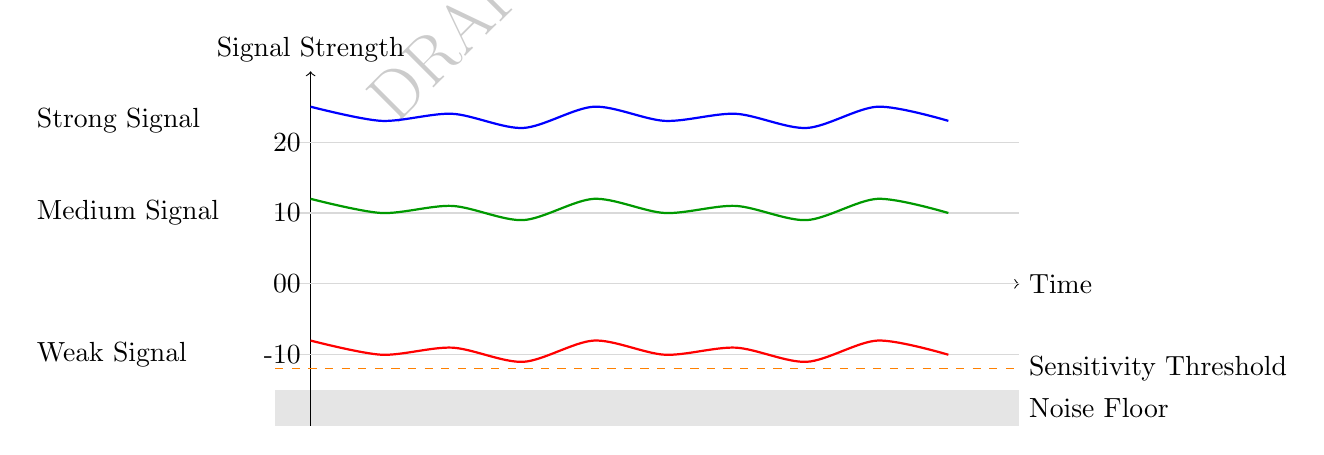
\begin{tikzpicture}[scale=0.9]
        % Define noise floor
        \fill[gray!20] (-0.5,-2) rectangle (10,-1.5);
        \node[right] at (10,-1.75) {Noise Floor};
        
        % Draw signal strength axis
        \draw[->] (-0.5,0) -- (10,0) node[right] {Time};
        \draw[->] (0,-2) -- (0,3) node[above] {Signal Strength};
        
        % Draw grid lines and labels
        \foreach \y in {-1,0,1,2} {
            \draw[gray!30] (-0.5,\y) -- (10,\y);
            \node[left] at (0,\y) {\y0};
        }
        
        % Draw three signals of different strengths
        \draw[thick,blue] plot[smooth] coordinates {
            (0,2.5) (1,2.3) (2,2.4) (3,2.2) (4,2.5) (5,2.3) (6,2.4) (7,2.2) (8,2.5) (9,2.3)
        };
        \node[right] at (-4,2.3) {Strong Signal};
        
        \draw[thick,green!60!black] plot[smooth] coordinates {
            (0,1.2) (1,1.0) (2,1.1) (3,0.9) (4,1.2) (5,1.0) (6,1.1) (7,0.9) (8,1.2) (9,1.0)
        };
        \node[right] at (-4,1.0) {Medium Signal};
        
        \draw[thick,red] plot[smooth] coordinates {
            (0,-0.8) (1,-1.0) (2,-0.9) (3,-1.1) (4,-0.8) (5,-1.0) (6,-0.9) (7,-1.1) (8,-0.8) (9,-1.0)
        };
        \node[right] at (-4,-1.0) {Weak Signal };
        
        % Draw sensitivity threshold
        \draw[dashed,orange] (-0.5,-1.2) -- (10,-1.2);
        \node[right] at (10,-1.2) {Sensitivity Threshold};
        
        
    \end{tikzpicture}
    \caption{Sensitivity in Radio Receivers: The diagram shows three signals of different strengths relative to the receiver's sensitivity threshold and noise floor. Signals must be above both the sensitivity threshold and noise floor to be detected reliably.}
    \label{fig:sensitivity-diagram}
\end{figure}

\subsubsection*{Selectivity: The Art of Ignoring Noise}
While sensitivity is about detecting weak signals, selectivity is about ignoring the ones you don’t want. Selectivity refers to the receiver’s ability to discriminate between multiple signals, especially those that are close in frequency. Imagine trying to listen to your favorite radio station while another station is broadcasting on a nearby frequency. A receiver with good selectivity can filter out the unwanted station, letting you enjoy your music without interference.

Selectivity is often measured in terms of bandwidth and rejection ratio. A narrower bandwidth generally means better selectivity, as it allows the receiver to focus on a smaller range of frequencies. The rejection ratio indicates how well the receiver can suppress signals outside its desired bandwidth.


\begin{figure}[h]
    \centering
    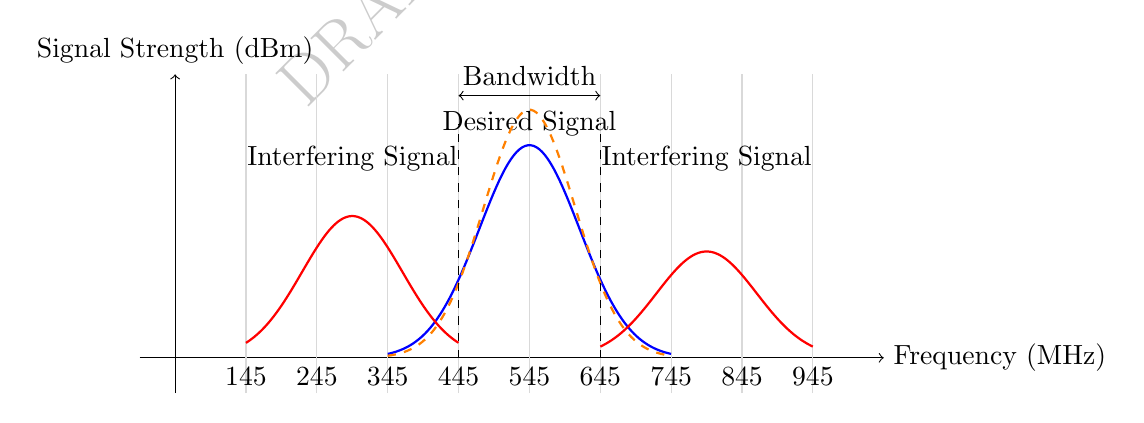
\begin{tikzpicture}[scale=0.9]
        % Draw axes
        \draw[->] (-0.5,0) -- (10,0) node[right] {Frequency (MHz)};
        \draw[->] (0,-0.5) -- (0,4) node[above] {Signal Strength (dBm)};
        
        % Draw grid lines
        \foreach \x in {1,2,3,4,5,6,7,8,9} {
            \draw[gray!30] (\x,-0.5) -- (\x,4);
            \node[below] at (\x,0) {\x45};
        }
        
        % Draw desired signal (center frequency)
        \draw[thick,blue] plot[domain=3:7,samples=100] 
            (\x,{3*exp(-(\x-5)*(\x-5))});
        \node[above] at (5,3) {Desired Signal};
        
        % Draw interfering signals
        \draw[thick,red] plot[domain=1:4,samples=100] 
            (\x,{2*exp(-(\x-2.5)*(\x-2.5))});
        \node[above] at (2.5,2.5) {Interfering Signal};
        
        \draw[thick,red] plot[domain=6:9,samples=100] 
            (\x,{1.5*exp(-(\x-7.5)*(\x-7.5))});
        \node[above] at (7.5,2.5) {Interfering Signal};
        
        % Draw selectivity filter response
        \draw[dashed,orange,thick] plot[domain=3:7,samples=100] 
            (\x,{3.5*exp(-1.2*(\x-5)*(\x-5))});
        % \node[below] at (11,2) {Filter Response};
        
        % Draw bandwidth markers
        \draw[<->] (4,3.7) -- (6,3.7) node[midway,above] {Bandwidth};
        \draw[dashed] (4,0) -- (4,3.3);
        \draw[dashed] (6,0) -- (6,3.3);
        
        % Add rejection ratio indicator
        % \draw[<->] (5,3) -- (5,0.5) node[midway,right] {Rejection Ratio};
        
        % Add explanatory text
        
    \end{tikzpicture}
    \caption{Selectivity in Radio Receivers: The diagram shows how a receiver's selectivity filter responds to signals at different frequencies. The desired signal (blue) passes through while interfering signals (red) are attenuated. The bandwidth determines the range of frequencies accepted.}
    \label{fig:selectivity-diagram}
\end{figure}

\subsubsection*{Sensitivity vs. Selectivity: A Friendly Rivalry}
While sensitivity and selectivity are both crucial for receiver performance, they often pull in opposite directions. A highly sensitive receiver might pick up weak signals, but it could also pick up more noise and interference. On the other hand, a highly selective receiver might filter out unwanted signals, but it could also miss some of the weaker ones. The key is to strike a balance between the two, depending on your specific needs.



\begin{table}[h]
    \centering
    \begin{tabular}{|l|l|l|}
        \hline
        \textbf{Parameter} & \textbf{Sensitivity} & \textbf{Selectivity} \\
        \hline
        Definition & Ability to detect weak signals & Ability to discriminate between signals \\
        \hline
        Measurement & Microvolts ($\mu V$) or dBm & Bandwidth and rejection ratio \\
        \hline
        Impact & Detects faint signals & Reduces interference \\
        \hline
    \end{tabular}
    \caption{Comparison of Sensitivity and Selectivity}
    \label{tab:sensitivity-selectivity}
\end{table}

\subsubsection{Questions}

\begin{tcolorbox}[colback=gray!10!white,colframe=black!75!black,title={T7A01}]
    Which term describes the ability of a receiver to detect the presence of a signal?
    \begin{enumerate}[label=\Alph*),noitemsep]
        \item Linearity
        \item \textbf{Sensitivity}
        \item Selectivity
        \item Total Harmonic Distortion
    \end{enumerate}
\end{tcolorbox}

Sensitivity is the term that describes a receiver's ability to detect weak signals. It is measured in microvolts or dBm, and a lower value indicates better sensitivity. The other options, such as linearity and total harmonic distortion, are related to different aspects of receiver performance.

\begin{tcolorbox}[colback=gray!10!white,colframe=black!75!black,title={T7A04}]
    Which term describes the ability of a receiver to discriminate between multiple signals?
    \begin{enumerate}[label=\Alph*),noitemsep]
        \item Discrimination ratio
        \item Sensitivity
        \item \textbf{Selectivity}
        \item Harmonic distortion
    \end{enumerate}
\end{tcolorbox}

Selectivity is the ability of a receiver to distinguish between multiple signals, especially those close in frequency. It is crucial for reducing interference. Sensitivity, on the other hand, is about detecting weak signals, while harmonic distortion is related to signal quality.

% \subsection{Mixer, Oscillator, Frequency Conversion}
\label{subsec:mixer-osc}

In this section, we'll dive into the fascinating world of mixers, oscillators, and frequency conversion. These components are the unsung heroes of radio technology, quietly working behind the scenes to make sure your signals get where they need to go. Let's break it down, shall we?

\subsubsection*{The Role of a Mixer}

A mixer is like the DJ of the radio world—it takes two signals and blends them together to create something new. Specifically, a mixer performs frequency conversion, which is essential for shifting signals from one frequency to another. This is crucial in radio systems because it allows us to transmit and receive signals at different frequencies without interference.

Imagine you have a signal at frequency \( f_1 \) and you want to convert it to frequency \( f_2 \). The mixer takes this signal and combines it with another signal from a local oscillator (more on that later) at frequency \( f_{LO} \). The result is a new signal at the sum or difference of these frequencies, typically \( f_1 + f_{LO} \) or \( f_1 - f_{LO} \). This process is known as heterodyning, and it's the backbone of frequency conversion in radio systems.

\subsubsection*{The Function of an Oscillator}

Now, let's talk about the oscillator. If the mixer is the DJ, the oscillator is the beat generator. It produces a signal at a specific frequency, which is then used by the mixer to perform frequency conversion. Oscillators are also key players in frequency synthesis and modulation, where they help generate the precise frequencies needed for various radio applications.

An oscillator circuit typically consists of an amplifier and a feedback loop that sustains the oscillation. The frequency of the output signal is determined by the components in the circuit, such as capacitors and inductors. This makes oscillators incredibly versatile, as they can be tuned to produce a wide range of frequencies.

\subsubsection*{Frequency Conversion: The Big Picture}

Frequency conversion is the process of changing a signal's frequency, and it's where mixers and oscillators come together in perfect harmony. The mixer takes the input signal and the oscillator's signal, and through the magic of heterodyning, produces a new signal at the desired frequency. This is essential in radio systems, where signals often need to be shifted to different frequencies for transmission, reception, or further processing.

For example, in a superheterodyne receiver, the incoming signal is mixed with a local oscillator signal to produce an intermediate frequency (IF) that's easier to process. This allows the receiver to be more selective and sensitive, improving overall performance.

\begin{figure}[h!]
    \centering
    % \includegraphics[width=0.8\textwidth]{mixer-diagram}
    \caption{Mixer Circuit Diagram}
    \label{fig:mixer-diagram}
    % Block diagram of a mixer circuit showing input, output, and local oscillator connections.
\end{figure}

\begin{figure}[h!]
    \centering
    % \includegraphics[width=0.8\textwidth]{oscillator-diagram}
    \caption{Oscillator Circuit Diagram}
    \label{fig:oscillator-diagram}
    % Diagram of an oscillator circuit generating a specific frequency signal.
\end{figure}

\begin{table}[h!]
    \centering
    \begin{tabular}{|l|l|}
        \hline
        \textbf{Component} & \textbf{Function} \\
        \hline
        Mixer & Performs frequency conversion by combining input signals with a local oscillator signal. \\
        Oscillator & Generates a signal at a specific frequency for use in frequency conversion and modulation. \\
        \hline
    \end{tabular}
    \caption{Mixer and Oscillator Functions}
    \label{tab:mixer-oscillator}
\end{table}

\subsubsection*{Questions}

\begin{tcolorbox}[colback=gray!10!white,colframe=black!75!black,title={T7A03}]
    Which of the following is used to convert a signal from one frequency to another?
    \begin{enumerate}[label=\Alph*),noitemsep]
        \item Phase splitter
        \item \textbf{Mixer}
        \item Inverter
        \item Amplifier
    \end{enumerate}
\end{tcolorbox}

A mixer is used to convert a signal from one frequency to another by combining it with a local oscillator signal. This process is known as heterodyning. The other options—phase splitter, inverter, and amplifier—do not perform frequency conversion.

\begin{tcolorbox}[colback=gray!10!white,colframe=black!75!black,title={T7A05}]
    What is the name of a circuit that generates a signal at a specific frequency?
    \begin{enumerate}[label=\Alph*),noitemsep]
        \item Reactance modulator
        \item Phase modulator
        \item Low-pass filter
        \item \textbf{Oscillator}
    \end{enumerate}
\end{tcolorbox}

An oscillator is a circuit that generates a signal at a specific frequency. Reactance modulators, phase modulators, and low-pass filters do not generate signals at specific frequencies; they modify or filter existing signals.

% \subsection{Transverter, PTT lines, etc.}
\label{subsec:transverter-ptt}

In this section, we'll explore the world of amplifiers, the driving forces of radio communication that ensure your signal reaches its destination. We'll cover essential components from transceivers to RF power amplifiers, including the important switches that keep everything running smoothly. This will be a brief overview of these topics, providing just enough information to help you pass the exam. We'll explore these topics in greater detail in subsequent books.

\subsubsection*{Transverter: The Frequency Shifter}
A transverter is a nifty device that converts the RF input and output of a transceiver to another band. Think of it as a translator for radio frequencies. If your transceiver operates on one band, but you need to communicate on another, the transverter steps in to make the conversion. It does this by mixing the incoming signal with a local oscillator signal, resulting in a new frequency that matches the desired band. This process is crucial for multi-band operations, allowing you to communicate across different frequency ranges without needing multiple transceivers.

\begin{figure}[h!]
    \centering
    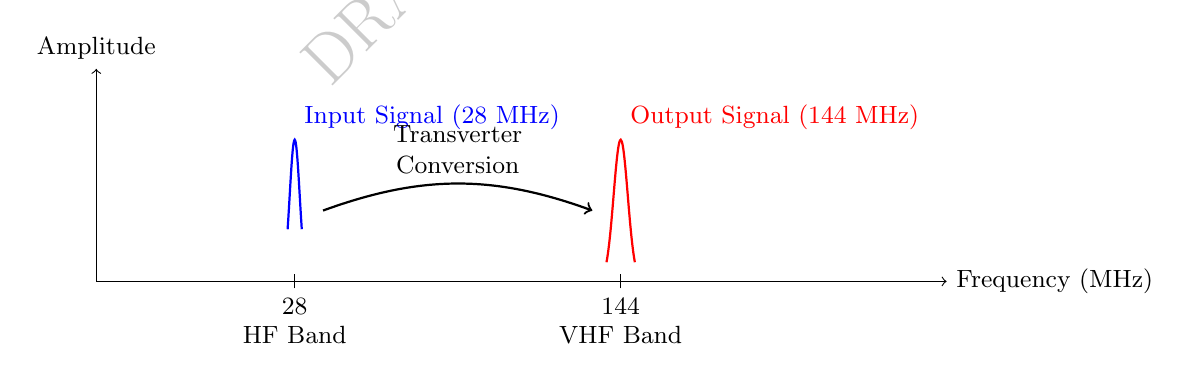
\begin{tikzpicture}[
        scale=0.9,
        every node/.style={font=\small}
    ]
        % Grid settings
        \def\ymax{3}
        \def\xmax{12}
        
        % Axes
        \draw[->] (0,0) -- (\xmax,0) node[right] {Frequency (MHz)};
        \draw[->] (0,0) -- (0,\ymax) node[above] {Amplitude};
        
        % Frequency markers
        \foreach \x/\label in {2.8/28, 7.4/144} {
            \draw (\x,-0.1) -- (\x,0.1);
            \node[below] at (\x,-0.1) {\label};
        }
        
        % Input signal at 28 MHz
        \draw[thick, blue] plot[domain=2.7:2.9,smooth] (\x,{2*exp(-100*(\x-2.8)*(\x-2.8))});
        \node[blue, above right] at (2.8,2) {Input Signal (28 MHz)};
        
        % Output signal at 144 MHz
        \draw[thick, red] plot[domain=7.2:7.6,smooth] (\x,{2*exp(-50*(\x-7.4)*(\x-7.4))});
        \node[red, above right] at (7.4,2) {Output Signal (144 MHz)};
        
        % Conversion arrow
        \draw[->, thick] (3.2,1) to[bend left=20] 
            node[midway, above, text width=2cm, align=center] {Transverter\\Conversion} (7,1);
            
        % Optional: Add frequency bands labels
        \node[below] at (2.8,-0.5) {HF Band};
        \node[below] at (7.4,-0.5) {VHF Band};
        
    \end{tikzpicture}
    \caption{Frequency spectrum showing signal conversion by a transverter from 28 MHz (HF) to 144 MHz (VHF) band}
    \label{fig:transverter-signals}
\end{figure}

\subsubsection*{PTT (Push-to-Talk): The Transmit/Receive Switch}
Next up is the PTT input, a critical feature in transceivers. The PTT input is what switches your transceiver from receive mode to transmit mode when grounded. In simpler terms, when you press the PTT button (usually on your microphone), it grounds the PTT input, telling the transceiver, "Hey, it's time to transmit!" When you release the button, the transceiver goes back to listening mode. This mechanism ensures that you're not transmitting and receiving at the same time, which would be... well, chaotic.


\subsubsection*{Modulation: The Voice of Radio}
Modulation is how we combine our voice or data with a radio signal for transmission. Think of it like writing a message, where we have three different ways to vary our writing:

\begin{itemize}[noitemsep]
    \item \textbf{Amplitude Modulation (AM):} Like changing how hard you press the pencil while writing. The height (strength) of the radio wave changes based on your voice - louder voice makes taller waves, softer voice makes shorter waves.
    
    \item \textbf{Frequency Modulation (FM):} Like changing how quickly you write each letter. The radio wave bunches up or spreads out based on your voice - louder parts make the waves bunch closer together, softer parts spread them apart.
    
    \item \textbf{Phase Modulation (PM):} Like slightly shifting each letter forward or backward while writing. The timing of each radio wave peak shifts slightly based on your voice - similar to FM but responds to how quickly your voice changes rather than its volume.
\end{itemize}

Each method has its advantages: AM is simple but picks up noise easily, FM gives better quality and is less affected by noise (which is why it's used for music radio), and PM is particularly useful for digital signals.

\begin{figure}[h!]
    \centering
    \includegraphics[width=0.9\textwidth]{images/modulations.png}
    \caption{Comparison of different modulation types: Amplitude Modulation (AM) varies the signal amplitude,  Frequency Modulation (FM) varies the signal frequency, and  Phase Modulation (PM) varies the signal phase according to the modulating signal}
    \label{fig:modulation-comparison}
\end{figure}


\subsubsection{Questions}
\begin{tcolorbox}[colback=gray!10!white,colframe=black!75!black,title={T7A06}]
    What device converts the RF input and output of a transceiver to another band?
    \begin{enumerate}[label=\Alph*),noitemsep]
        \item High-pass filter
        \item Low-pass filter
        \item \textbf{Transverter}
        \item Phase converter
    \end{enumerate}
\end{tcolorbox}
A transverter is specifically designed to convert RF signals from one band to another, making it the correct answer. High-pass and low-pass filters are used to filter frequencies, not convert them, and a phase converter is unrelated to frequency conversion.

\begin{tcolorbox}[colback=gray!10!white,colframe=black!75!black,title={T7A07}]
    What is the function of a transceiver’s PTT input?
    \begin{enumerate}[label=\Alph*),noitemsep]
        \item Input for a key used to send CW
        \item \textbf{Switches transceiver from receive to transmit when grounded}
        \item Provides a transmit tuning tone when grounded
        \item Input for a preamplifier tuning tone
    \end{enumerate}
\end{tcolorbox}
The PTT input is used to switch the transceiver from receive to transmit mode when grounded. It’s not related to CW keys, tuning tones, or preamplifiers.

\begin{tcolorbox}[colback=gray!10!white,colframe=black!75!black,title={T7A08}]
    Which of the following describes combining speech with an RF carrier signal?
    \begin{enumerate}[label=\Alph*),noitemsep]
        \item Impedance matching
        \item Oscillation
        \item \textbf{Modulation}
        \item Low-pass filtering
    \end{enumerate}
\end{tcolorbox}
Modulation is the process of combining speech with an RF carrier signal. Impedance matching, oscillation, and low-pass filtering are unrelated to this process.

% \section{RF Power Amplifiers and Preamps}
% \subsection{Amplifier Basics}
\label{subsec:amp-basics}

In this section, we'll dive into the world of amplifiers, those driving forces of the radio world that make sure your signal gets where it needs to go. We'll cover everything from transceivers to RF power amplifiers, and even touch on those nifty little switches that make sure everything runs smoothly. We will only have a shallow dip on these topics just enough to get you through the exam. In the next books we will dive deeper into these topics.

\subsubsection*{Transceiver: The Jack of All Trades}
A transceiver is like the Swiss Army knife of radio equipment. It combines both a receiver and a transmitter into a single device, making it incredibly versatile. Imagine trying to juggle two separate devices every time you wanted to switch between sending and receiving signals—sounds like a nightmare, right? Well, that's exactly what a transceiver saves you from. It seamlessly integrates both functions, allowing you to communicate efficiently without breaking a sweat.


\subsubsection*{The SSB/CW-FM Switch: Mode Master}
Ever wondered how a VHF power amplifier knows whether you're in Single Sideband (SSB), Continuous Wave (CW), or Frequency Modulation (FM) mode? Enter the SSB/CW-FM switch. This little guy ensures that your amplifier is set up correctly for the mode you're operating in. It doesn't change the mode itself—that's your job—but it makes sure the amplifier is optimized for whatever mode you've chosen. Think of it as the amplifier's personal trainer, keeping it in tip-top shape for whatever you throw at it.


\subsubsection*{RF Power Amplifier: The Muscle}
If your transceiver is the brain, then the RF power amplifier is the brawn. This device takes the relatively weak signal from your transceiver and boosts it to a level that can be transmitted over long distances. Without it, your signal might not even make it out of your backyard. So, if you're looking to reach someone on the other side of the world, you'll want to make sure your RF power amplifier is up to the task.


\subsubsection*{RF Preamplifier: The First Responder}
The RF preamplifier is the first line of defense in your signal reception process. It's installed between the antenna and the receiver, and its job is to amplify weak signals before they reach the receiver. This is crucial because weak signals can easily get lost in the noise, making them impossible to decode. By boosting these signals early on, the RF preamplifier ensures that your receiver has a fighting chance of picking them up.


\begin{table}[h!]
    \centering
    \begin{tabular}{|l|l|}
        \hline
        \textbf{Device} & \textbf{Function} \\
        \hline
        Transceiver & Combines receiver and transmitter into a single device \\
        RF Power Amplifier & Boosts the transmitted signal from the transceiver \\
        RF Preamplifier & Amplifies weak signals before they reach the receiver \\
        \hline
    \end{tabular}
    \caption{Comparison of transceiver, RF power amplifier, and RF preamplifier functions.}
    \label{tab:comparison-functions}
\end{table}

\subsubsection*{Questions}

\begin{tcolorbox}[colback=gray!10!white,colframe=black!75!black,title={T7A02}]
    What is a transceiver?
    \begin{enumerate}[label=\Alph*),noitemsep]
        \item \textbf{A device that combines a receiver and transmitter}
        \item A device for matching feed line impedance to 50 ohms
        \item A device for automatically sending and decoding Morse code
        \item A device for converting receiver and transmitter frequencies to another band
    \end{enumerate}
\end{tcolorbox}

A transceiver is a device that combines both a receiver and a transmitter into a single unit. This integration allows for seamless switching between sending and receiving signals, making it a versatile tool in radio communication. The other options describe different devices or functions that are not related to the definition of a transceiver.

\begin{tcolorbox}[colback=gray!10!white,colframe=black!75!black,title={T7A09}]
    What is the function of the SSB/CW-FM switch on a VHF power amplifier?
    \begin{enumerate}[label=\Alph*),noitemsep]
        \item Change the mode of the transmitted signal
        \item \textbf{Set the amplifier for proper operation in the selected mode}
        \item Change the frequency range of the amplifier to operate in the proper segment of the band
        \item Reduce the received signal noise
    \end{enumerate}
\end{tcolorbox}

The SSB/CW-FM switch on a VHF power amplifier ensures that the amplifier is configured correctly for the mode you're operating in. It doesn't change the mode itself but optimizes the amplifier's settings for SSB, CW, or FM modes. The other options describe functions that are either unrelated or incorrect for this specific switch.

\begin{tcolorbox}[colback=gray!10!white,colframe=black!75!black,title={T7A10}]
    What device increases the transmitted output power from a transceiver?
    \begin{enumerate}[label=\Alph*),noitemsep]
        \item A voltage divider
        \item \textbf{An RF power amplifier}
        \item An impedance network
        \item All these choices are correct
    \end{enumerate}
\end{tcolorbox}

An RF power amplifier is specifically designed to increase the transmitted output power from a transceiver. Voltage dividers and impedance networks serve different purposes and do not amplify signals. Therefore, the correct answer is B.

\begin{tcolorbox}[colback=gray!10!white,colframe=black!75!black,title={T7A11}]
    Where is an RF preamplifier installed?
    \begin{enumerate}[label=\Alph*),noitemsep]
        \item \textbf{Between the antenna and receiver}
        \item At the output of the transmitter power amplifier
        \item Between the transmitter and the antenna tuner
        \item At the output of the receiver audio amplifier
    \end{enumerate}
\end{tcolorbox}

An RF preamplifier is installed between the antenna and the receiver to amplify weak signals before they reach the receiver. This placement ensures that the signals are strong enough to be processed effectively. The other options describe incorrect locations for an RF preamplifier.

% \chapter{Power Supplies, Cables, and Station Setup}
% \section{Power Supplies}
% \subsection{Choosing and Using}
\label{subsec:psu-choice}

When it comes to setting up your radio station, choosing the right components is crucial. Let's dive into some key considerations for selecting and using various equipment, from power supplies to digital mode interfaces.

\subsubsection*{Power Supply Ratings}
Selecting the correct power supply for your mobile FM transceiver is like choosing the right fuel for your car—get it wrong, and you're not going anywhere fast. The power supply must match the voltage and current requirements of your transceiver to ensure optimal performance. For a typical 50-watt output mobile FM transceiver, you'll need a power supply that can deliver 13.8 volts at 12 amperes. This ensures that your transceiver gets the juice it needs without overloading the power supply.

\subsubsection*{SWR Meter Selection}
An SWR meter is your best friend when it comes to tuning your antenna. But not all SWR meters are created equal. When selecting one, consider the frequency and power level at which you'll be making measurements. A meter that works great at low power might not cut it when you crank up the watts. Always check the specifications to ensure the meter can handle your station's requirements.

\subsubsection*{DC Power Connection Wires}
Ever wonder why those wires connecting your transceiver to the power supply are so short and thick? It's all about minimizing voltage drop. When you're transmitting, your transceiver draws a lot of current, and if the wires are too long or too thin, you'll lose voltage along the way. Short, heavy-gauge wires ensure that your transceiver gets the full voltage it needs, keeping your signal strong and clear.

\subsubsection*{FT8 Configuration}
FT8 is a popular digital mode, and setting it up requires a bit of know-how. The transceiver's audio input and output need to be connected to a computer running WSJT-X software. This setup allows the computer to handle the digital encoding and decoding, while the transceiver takes care of the RF side of things. It's a match made in ham radio heaven.

\subsubsection*{RF Power Meter Installation}
An RF power meter is like the speedometer for your transmitter. It tells you how much power is actually making it to the antenna. For accurate readings, install the meter in the feed line between the transmitter and the antenna. This placement ensures that you're measuring the power that's actually being radiated, not just what's coming out of the transmitter.

\subsubsection*{Computer-Radio Interface Signals}
When operating digital modes, your computer and transceiver need to talk to each other. This communication happens through a few key signals: receive audio, transmit audio, and transmitter keying. These signals allow the computer to control the transceiver and process the digital data, making modern digital modes possible.

\subsubsection*{Digital Mode Connections}
Connecting your computer to your transceiver for digital mode operation isn't as complicated as it sounds. The key is to connect the computer's "line in" to the transceiver's speaker connector. This setup allows the computer to receive audio from the transceiver and send audio back for transmission. It's a simple but effective way to bridge the gap between your computer and your radio.

\subsubsection*{RF Bonding Conductors}
When it comes to bonding at RF frequencies, not all conductors are created equal. Flat copper strap is the preferred choice because it offers low impedance and excellent conductivity. Other materials, like steel wire or twisted-pair cable, just don't cut it when you're dealing with high-frequency signals.

\subsubsection*{Battery Runtime Calculation}
Calculating how long your equipment can run on a battery is a handy skill. The formula is simple: divide the battery's ampere-hour rating by the average current draw of your equipment. This gives you the runtime in hours. For example, a 20 Ah battery powering a transceiver that draws 2 A on average will last about 10 hours.

\subsubsection*{Digital Mode Hot Spot Function}
A digital mode hot spot is like a mini repeater for digital voice and data communication. It connects your transceiver to the internet, allowing you to communicate with other hams around the world using digital modes. It's a game-changer for anyone looking to expand their digital horizons.

\subsubsection*{Mobile Transceiver Grounding}
Proper grounding is essential for a mobile transceiver. The negative power return should be connected to the vehicle's 12-volt battery chassis ground. This ensures a solid ground connection, reducing noise and improving performance. Don't skimp on this step—your signal will thank you.

\subsubsection*{Electronic Keyer}
An electronic keyer is a handy tool for Morse code enthusiasts. It assists in manual sending by automating the timing of dots and dashes, making your code more consistent and easier to read. It's a must-have for anyone serious about CW operation.

\begin{figure}[h!]
    \centering
    % \includegraphics[width=0.8\textwidth]{power-supply-relationship.svg}
    \caption{Power Supply Voltage and Current Relationship}
    \label{fig:power-supply-relationship}
    % Diagram showing the relationship between voltage, current, and power in a mobile FM transceiver power supply.
\end{figure}

\begin{figure}[h!]
    \centering
    % \includegraphics[width=0.8\textwidth]{rf-power-meter-installation.svg}
    \caption{RF Power Meter Installation}
    \label{fig:rf-power-meter-installation}
    % Illustration of a station setup with an RF power meter installed in the feed line between the transmitter and antenna.
\end{figure}

\begin{figure}[h!]
    \centering
    % \includegraphics[width=0.8\textwidth]{computer-radio-interface.svg}
    \caption{Computer-Radio Interface for Digital Modes}
    \label{fig:computer-radio-interface}
    % Diagram of a computer-radio interface for digital mode operation, showing audio and keying signal connections.
\end{figure}

\begin{table}[h!]
    \centering
    \begin{tabular}{|l|l|l|}
        \hline
        \textbf{Conductor Type} & \textbf{Advantages} & \textbf{Disadvantages} \\
        \hline
        Flat Copper Strap & Low impedance, excellent conductivity & Bulkier, harder to bend \\
        Copper Braid & Flexible, easy to route & Higher impedance \\
        Steel Wire & Strong, durable & Poor conductivity \\
        Twisted-Pair Cable & Good for low-frequency signals & Not suitable for RF \\
        \hline
    \end{tabular}
    \caption{Comparison of RF Bonding Conductors}
    \label{tab:rf-bonding-conductors}
\end{table}

\begin{table}[h!]
    \centering
    \begin{tabular}{|l|l|}
        \hline
        \textbf{Battery Ampere-Hour Rating} & \textbf{Runtime (hours)} \\
        \hline
        10 Ah & 5 \\
        20 Ah & 10 \\
        30 Ah & 15 \\
        40 Ah & 20 \\
        \hline
    \end{tabular}
    \caption{Battery Runtime Calculation}
    \label{tab:battery-runtime-calculation}
\end{table}

\subsubsection*{Questions}

\begin{tcolorbox}[colback=gray!10!white,colframe=black!75!black,title={T4A01}]
    Which of the following is an appropriate power supply rating for a typical 50 watt output mobile FM transceiver?
    \begin{enumerate}[label=\Alph*),noitemsep]
        \item 24.0 volts at 4 amperes
        \item 13.8 volts at 4 amperes
        \item 24.0 volts at 12 amperes
        \item \textbf{13.8 volts at 12 amperes}
    \end{enumerate}
\end{tcolorbox}
A 50-watt transceiver typically requires a power supply that can deliver 13.8 volts at 12 amperes. This ensures that the transceiver receives sufficient power without overloading the supply.

\begin{tcolorbox}[colback=gray!10!white,colframe=black!75!black,title={T4A02}]
    Which of the following should be considered when selecting an accessory SWR meter?
    \begin{enumerate}[label=\Alph*),noitemsep]
        \item \textbf{The frequency and power level at which the measurements will be made}
        \item The distance that the meter will be located from the antenna
        \item The types of modulation being used at the station
        \item All these choices are correct
    \end{enumerate}
\end{tcolorbox}
The frequency and power level are critical factors when selecting an SWR meter. The meter must be capable of handling the specific frequency and power levels at which you'll be operating.

\begin{tcolorbox}[colback=gray!10!white,colframe=black!75!black,title={T4A03}]
    Why are short, heavy-gauge wires used for a transceiver’s DC power connection?
    \begin{enumerate}[label=\Alph*),noitemsep]
        \item \textbf{To minimize voltage drop when transmitting}
        \item To provide a good counterpoise for the antenna
        \item To avoid RF interference
        \item All these choices are correct
    \end{enumerate}
\end{tcolorbox}
Short, heavy-gauge wires minimize voltage drop, ensuring that the transceiver receives the full voltage it needs during transmission.

\begin{tcolorbox}[colback=gray!10!white,colframe=black!75!black,title={T4A04}]
    How are the transceiver audio input and output connected in a station configured to operate using FT8?
    \begin{enumerate}[label=\Alph*),noitemsep]
        \item To a computer running a terminal program and connected to a terminal node controller unit
        \item \textbf{To the audio input and output of a computer running WSJT-X software}
        \item To an FT8 conversion unit, a keyboard, and a computer monitor
        \item To a computer connected to the FT8converter.com website
    \end{enumerate}
\end{tcolorbox}
For FT8 operation, the transceiver's audio input and output are connected to a computer running WSJT-X software, which handles the digital encoding and decoding.

\begin{tcolorbox}[colback=gray!10!white,colframe=black!75!black,title={T4A05}]
    Where should an RF power meter be installed?
    \begin{enumerate}[label=\Alph*),noitemsep]
        \item \textbf{In the feed line, between the transmitter and antenna}
        \item At the power supply output
        \item In parallel with the push-to-talk line and the antenna
        \item In the power supply cable, as close as possible to the radio
    \end{enumerate}
\end{tcolorbox}
An RF power meter should be installed in the feed line between the transmitter and the antenna to accurately measure the power being radiated.

\begin{tcolorbox}[colback=gray!10!white,colframe=black!75!black,title={T4A06}]
    What signals are used in a computer-radio interface for digital mode operation?
    \begin{enumerate}[label=\Alph*),noitemsep]
        \item Receive and transmit mode, status, and location
        \item Antenna and RF power
        \item \textbf{Receive audio, transmit audio, and transmitter keying}
        \item NMEA GPS location and DC power
    \end{enumerate}
\end{tcolorbox}
The key signals used in a computer-radio interface for digital modes are receive audio, transmit audio, and transmitter keying.

\begin{tcolorbox}[colback=gray!10!white,colframe=black!75!black,title={T4A07}]
    Which of the following connections is made between a computer and a transceiver to use computer software when operating digital modes?
    \begin{enumerate}[label=\Alph*),noitemsep]
        \item Computer “line out” to transceiver push-to-talk
        \item Computer “line in” to transceiver push-to-talk
        \item \textbf{Computer “line in” to transceiver speaker connector}
        \item Computer “line out” to transceiver speaker connector
    \end{enumerate}
\end{tcolorbox}
For digital mode operation, connect the computer's "line in" to the transceiver's speaker connector to allow the computer to receive audio from the transceiver.

\begin{tcolorbox}[colback=gray!10!white,colframe=black!75!black,title={T4A08}]
    Which of the following conductors is preferred for bonding at RF?
    \begin{enumerate}[label=\Alph*),noitemsep]
        \item Copper braid removed from coaxial cable
        \item Steel wire
        \item Twisted-pair cable
        \item \textbf{Flat copper strap}
    \end{enumerate}
\end{tcolorbox}
Flat copper strap is preferred for RF bonding due to its low impedance and excellent conductivity.

\begin{tcolorbox}[colback=gray!10!white,colframe=black!75!black,title={T4A09}]
    How can you determine the length of time that equipment can be powered from a battery?
    \begin{enumerate}[label=\Alph*),noitemsep]
        \item Divide the watt-hour rating of the battery by the peak power consumption of the equipment
        \item \textbf{Divide the battery ampere-hour rating by the average current draw of the equipment}
        \item Multiply the watts per hour consumed by the equipment by the battery power rating
        \item Multiply the square of the current rating of the battery by the input resistance of the equipment
    \end{enumerate}
\end{tcolorbox}
To calculate battery runtime, divide the battery's ampere-hour rating by the average current draw of the equipment.

\begin{tcolorbox}[colback=gray!10!white,colframe=black!75!black,title={T4A10}]
    What function is performed with a transceiver and a digital mode hot spot?
    \begin{enumerate}[label=\Alph*),noitemsep]
        \item \textbf{Communication using digital voice or data systems via the internet}
        \item FT8 digital communications via AFSK
        \item RTTY encoding and decoding without a computer
        \item High-speed digital communications for meteor scatter
    \end{enumerate}
\end{tcolorbox}
A digital mode hot spot enables communication using digital voice or data systems via the internet.

\begin{tcolorbox}[colback=gray!10!white,colframe=black!75!black,title={T4A11}]
    Where should the negative power return of a mobile transceiver be connected in a vehicle?
    \begin{enumerate}[label=\Alph*),noitemsep]
        \item \textbf{At the 12 volt battery chassis ground}
        \item At the antenna mount
        \item To any metal part of the vehicle
        \item Through the transceiver’s mounting bracket
    \end{enumerate}
\end{tcolorbox}
The negative power return of a mobile transceiver should be connected to the vehicle's 12-volt battery chassis ground for proper grounding.

\begin{tcolorbox}[colback=gray!10!white,colframe=black!75!black,title={T4A12}]
    What is an electronic keyer?
    \begin{enumerate}[label=\Alph*),noitemsep]
        \item A device for switching antennas from transmit to receive
        \item A device for voice activated switching from receive to transmit
        \item \textbf{A device that assists in manual sending of Morse code}
        \item An interlock to prevent unauthorized use of a radio
    \end{enumerate}
\end{tcolorbox}
An electronic keyer assists in manual sending of Morse code by automating the timing of dots and dashes.

% \section{Radio/Audio Controls}
% \subsection{Mic Gain, Squelch, etc.}
\label{subsec:mic-squelch}

In this section, we'll dive into some of the finer details of radio operation, focusing on microphone gain, squelch, and other related concepts. These might seem like small details, but trust me, they can make a big difference in your radio experience. So, let's get started!

\subsubsection*{Microphone Gain and SSB Transmissions}

Microphone gain is essentially how sensitive your microphone is to your voice. Think of it like turning up the volume on your voice before it even hits the transmitter. While this might sound like a good thing, too much gain can lead to distorted audio. Imagine shouting into a microphone—your voice might start to sound like a robot or, worse, like you're underwater. This is because excessive gain can cause the audio signal to clip, leading to distortion. In SSB (Single Sideband) transmissions, this distortion can make your signal hard to understand, which is the last thing you want when you're trying to communicate clearly.

\begin{figure}[h]
    \centering
    % \includegraphics[width=0.8\textwidth]{figures/mic-gain-distortion}
    \caption{Impact of Microphone Gain on SSB Transmissions}

    \label{fig:mic-gain-distortion}
    % Diagram showing the relationship between microphone gain and audio distortion in SSB transmissions
\end{figure}

\subsubsection*{Frequency Entry Methods}

When it comes to entering frequencies on your transceiver, you have a few options. The most common methods are using the keypad or the VFO (Variable Frequency Oscillator) knob. The keypad is straightforward—just punch in the frequency you want. The VFO knob, on the other hand, lets you scroll through frequencies manually. Both methods have their pros and cons, but they’re generally more user-friendly than other techniques like CTCSS or DTMF encoding, which are more specialized.

\begin{figure}[h]
    \centering
    % \includegraphics[width=0.8\textwidth]{figures/frequency-entry}
    \caption{Frequency Entry Methods on a Transceiver}
    \label{fig:frequency-entry}
    % Illustration of a transceiver's keypad and VFO knob for frequency entry
\end{figure}

\subsubsection*{Squelch and Weak FM Signals}

Squelch is like a gatekeeper for your receiver. It keeps the noise out when there’s no signal, but lets the signal through when it’s strong enough. Adjusting the squelch threshold is crucial for hearing weak FM signals. If you set it too high, you might miss a faint signal. Set it too low, and you’ll be bombarded with noise. The trick is to find that sweet spot where the receiver output audio is just barely on all the time, allowing you to catch those weak signals without the constant hiss of background noise.

\begin{figure}[h]
    \centering
    % \includegraphics[width=0.8\textwidth]{figures/squelch-threshold}
    \caption{Squelch Threshold Adjustment for Weak FM Signals}
    \label{fig:squelch-threshold}
    % Graph showing the effect of squelch threshold adjustment on weak FM signal reception
\end{figure}

\subsubsection*{Memory Channels}

Memory channels are a lifesaver when you want quick access to your favorite frequencies. Instead of manually entering the frequency every time, you can store it in a memory channel and recall it with a single button press. It’s like having a speed dial for your radio. This is especially handy when you’re in the middle of an intense QSO (conversation) and don’t want to fumble with the keypad.

\begin{figure}[h]
    \centering
    % \includegraphics[width=0.8\textwidth]{figures/memory-channel}
    \caption{Memory Channel Interface for Quick Frequency Access}
    \label{fig:memory-channel}
    % Diagram of a transceiver's memory channel interface for quick frequency access
\end{figure}

\subsubsection*{Scanning Function}

The scanning function in FM transceivers is like having a radar for radio frequencies. It tunes through a range of frequencies to check for activity, which is incredibly useful when you’re trying to find someone to talk to or monitoring a busy channel. It’s like flipping through radio stations, but for ham radio. This feature is particularly handy in environments where frequencies are constantly changing, like during a contest or emergency situation.

\begin{figure}[h]
    \centering
    % \includegraphics[width=0.8\textwidth]{figures/scanning-function}
    \caption{FM Transceiver Scanning Function}
    \label{fig:scanning-function}
    % Flowchart of the scanning function in an FM transceiver
\end{figure}

\subsubsection*{RIT/Clarifier}

The RIT (Receiver Incremental Tuning) or Clarifier is your best friend when dealing with SSB signals that sound a bit off. If the voice pitch of a returning signal seems too high or low, you can use the RIT/Clarifier to fine-tune the frequency and correct the pitch. It’s like adjusting the tuning on a guitar—just a little twist can make all the difference.

\begin{figure}[h]
    \centering
    % \includegraphics[width=0.8\textwidth]{figures/rit-clarifier}
    \caption{RIT/Clarifier in SSB Signal Pitch Adjustment}
    \label{fig:rit-clarifier}
    % Diagram illustrating the use of RIT/Clarifier in SSB signal pitch adjustment
\end{figure}

\subsubsection*{DMR Code Plug}

A DMR (Digital Mobile Radio) code plug is essentially a configuration file that contains all the necessary information for your DMR transceiver to operate. This includes access information for repeaters and talkgroups. Think of it as the brain of your DMR radio—without it, your radio wouldn’t know where to connect or how to communicate.

\begin{figure}[h]
    \centering
    % \includegraphics[width=0.8\textwidth]{figures/dmr-code-plug}
    \caption{Contents of a DMR Code Plug}
    \label{fig:dmr-code-plug}
    % Illustration of a DMR code plug and its contents
\end{figure}

\subsubsection*{Receive Bandwidth}

Receive bandwidth is all about finding the right balance between signal clarity and noise reduction. Different modes require different bandwidth settings. For example, a narrower bandwidth might be better for reducing noise, but it could also cut out some of the signal’s detail. On the other hand, a wider bandwidth might give you more detail, but at the cost of increased noise. It’s a trade-off, and finding the right setting can make a big difference in your reception quality.

\begin{figure}[h]
    \centering
    % \includegraphics[width=0.8\textwidth]{figures/receive-bandwidth}
    \caption{Receive Bandwidth Settings and Noise Reduction}
    \label{fig:receive-bandwidth}
    % Graph comparing different receive bandwidth settings and their impact on noise reduction
\end{figure}

\subsubsection*{Digital Voice Group Selection}

Selecting a specific group of stations on a digital voice transceiver is usually done by entering the group’s identification code. This is particularly useful in digital communication, where you might want to talk to a specific group of people without broadcasting to everyone. It’s like having a private chat room within the larger network.

\begin{figure}[h]
    \centering
    % \includegraphics[width=0.8\textwidth]{figures/group-selection}
    \caption{Group Selection on a Digital Voice Transceiver}
    \label{fig:group-selection}
    % Diagram showing the process of selecting a group of stations on a digital voice transceiver
\end{figure}

\subsubsection*{Receiver Filter Bandwidth}

The receiver filter bandwidth plays a crucial role in SSB reception. A wider bandwidth might give you a better signal-to-noise ratio, but it could also let in more noise. Conversely, a narrower bandwidth might reduce noise, but it could also cut out some of the signal’s detail. The key is to find the right balance for your specific situation.

\begin{figure}[h]
    \centering
    % \includegraphics[width=0.8\textwidth]{figures/filter-bandwidth}
    \caption{Receiver Filter Bandwidth and Signal-to-Noise Ratio}
    \label{fig:filter-bandwidth}
    % Graph showing the relationship between receiver filter bandwidth and signal-to-noise ratio in SSB reception
\end{figure}

\subsubsection*{D-STAR Configuration}

Before you can transmit on a D-STAR digital transceiver, you need to program your call sign into the device. This is a crucial step, as it ensures that your transmissions are properly identified. Without this configuration, your radio might not even transmit, or worse, it could transmit without proper identification, which is a big no-no in the ham radio world.

\begin{figure}[h]
    \centering
    % \includegraphics[width=0.8\textwidth]{figures/dstar-config}
    \caption{D-STAR Transceiver Configuration Interface}
    \label{fig:dstar-config}
    % Diagram of a D-STAR transceiver configuration interface
\end{figure}

\subsubsection*{FM Receiver Tuning}

Tuning an FM receiver above or below a signal’s frequency can have some interesting effects. If you tune too far, you might hear a change in the audio pitch, or even some distortion. This is because the receiver is no longer perfectly aligned with the signal’s frequency, leading to a loss of clarity. It’s like trying to listen to a radio station that’s just slightly out of range—you might catch some of it, but it won’t be crystal clear.

\begin{figure}[h]
    \centering
    % \includegraphics[width=0.8\textwidth]{figures/fm-tuning}
    \caption{Effects of FM Receiver Tuning}
    \label{fig:fm-tuning}
    % Graph illustrating the effects of tuning an FM receiver above or below a signal's frequency
\end{figure}

\subsubsection*{Tables}

\begin{table}[h]
    \centering
    \caption{Comparison of Receiver Filter Bandwidths for SSB Reception}
    \label{tab:filter-bandwidth-comparison}
    \begin{tabular}{|c|c|}
        \hline
        \textbf{Bandwidth (Hz)} & \textbf{Impact on SSB Reception} \\
        \hline
        500 & Narrow, reduces noise but may cut signal detail \\
        1000 & Moderate, balances noise reduction and signal clarity \\
        2400 & Wide, better signal-to-noise ratio but more noise \\
        5000 & Very wide, maximum detail but highest noise \\
        \hline
    \end{tabular}
\end{table}

\begin{table}[h]
    \centering
    \caption{Effects of Excessive Microphone Gain on SSB Transmissions}
    \label{tab:mic-gain-effects}
    \begin{tabular}{|c|c|}
        \hline
        \textbf{Microphone Gain Level} & \textbf{Effect on SSB Transmissions} \\
        \hline
        Low & Clear audio, but may be too quiet \\
        Moderate & Optimal balance of clarity and volume \\
        High & Distorted audio, clipping, and reduced intelligibility \\
        \hline
    \end{tabular}
\end{table}

\subsubsection*{Questions}

\begin{tcolorbox}[colback=gray!10!white,colframe=black!75!black,title={T4B01}]
    What is the effect of excessive microphone gain on SSB transmissions?
    \begin{enumerate}[label=\Alph*),noitemsep]
        \item Frequency instability
        \item \textbf{Distorted transmitted audio}
        \item Increased SWR
        \item All these choices are correct
    \end{enumerate}
\end{tcolorbox}

Excessive microphone gain can cause the audio signal to clip, leading to distorted transmitted audio. This distortion makes the signal hard to understand, which is problematic for clear communication.

\begin{tcolorbox}[colback=gray!10!white,colframe=black!75!black,title={T4B02}]
    Which of the following can be used to enter a transceiver’s operating frequency?
    \begin{enumerate}[label=\Alph*),noitemsep]
        \item \textbf{The keypad or VFO knob}
        \item The CTCSS or DTMF encoder
        \item The Automatic Frequency Control
        \item All these choices are correct
    \end{enumerate}
\end{tcolorbox}

The keypad or VFO knob are the most common methods for entering a transceiver’s operating frequency. Other methods like CTCSS or DTMF encoding are more specialized and not typically used for frequency entry.

\begin{tcolorbox}[colback=gray!10!white,colframe=black!75!black,title={T4B03}]
    How is squelch adjusted so that a weak FM signal can be heard?
    \begin{enumerate}[label=\Alph*),noitemsep]
        \item \textbf{Set the squelch threshold so that receiver output audio is on all the time}
        \item Turn up the audio level until it overcomes the squelch threshold
        \item Turn on the anti-squelch function
        \item Enable squelch enhancement
    \end{enumerate}
\end{tcolorbox}

Setting the squelch threshold so that the receiver output audio is on all the time allows weak FM signals to be heard without being drowned out by noise.

\begin{tcolorbox}[colback=gray!10!white,colframe=black!75!black,title={T4B04}]
    What is a way to enable quick access to a favorite frequency or channel on your transceiver?
    \begin{enumerate}[label=\Alph*),noitemsep]
        \item Enable the frequency offset
        \item \textbf{Store it in a memory channel}
        \item Enable the VOX
        \item Use the scan mode to select the desired frequency
    \end{enumerate}
\end{tcolorbox}

Storing a favorite frequency in a memory channel allows for quick and easy access, making it much more convenient than manually entering the frequency each time.

\begin{tcolorbox}[colback=gray!10!white,colframe=black!75!black,title={T4B05}]
    What does the scanning function of an FM transceiver do?
    \begin{enumerate}[label=\Alph*),noitemsep]
        \item Checks incoming signal deviation
        \item Prevents interference to nearby repeaters
        \item \textbf{Tunes through a range of frequencies to check for activity}
        \item Checks for messages left on a digital bulletin board
    \end{enumerate}
\end{tcolorbox}

The scanning function tunes through a range of frequencies to check for activity, which is useful for monitoring multiple channels or finding active frequencies.

\begin{tcolorbox}[colback=gray!10!white,colframe=black!75!black,title={T4B06}]
    Which of the following controls could be used if the voice pitch of a single-sideband signal returning to your CQ call seems too high or low?
    \begin{enumerate}[label=\Alph*),noitemsep]
        \item The AGC or limiter
        \item The bandwidth selection
        \item The tone squelch
        \item \textbf{The RIT or Clarifier}
    \end{enumerate}
\end{tcolorbox}

The RIT (Receiver Incremental Tuning) or Clarifier can be used to adjust the pitch of an SSB signal, ensuring that the voice sounds natural and clear.

\begin{tcolorbox}[colback=gray!10!white,colframe=black!75!black,title={T4B07}]
    What does a DMR “code plug” contain?
    \begin{enumerate}[label=\Alph*),noitemsep]
        \item Your call sign in CW for automatic identification
        \item \textbf{Access information for repeaters and talkgroups}
        \item The codec for digitizing audio
        \item The DMR software version
    \end{enumerate}
\end{tcolorbox}

A DMR code plug contains access information for repeaters and talkgroups, which is essential for configuring your DMR transceiver.

\begin{tcolorbox}[colback=gray!10!white,colframe=black!75!black,title={T4B08}]
    What is the advantage of having multiple receive bandwidth choices on a multimode transceiver?
    \begin{enumerate}[label=\Alph*),noitemsep]
        \item Permits monitoring several modes at once by selecting a separate filter for each mode
        \item \textbf{Permits noise or interference reduction by selecting a bandwidth matching the mode}
        \item Increases the number of frequencies that can be stored in memory
        \item Increases the amount of offset between receive and transmit frequencies
    \end{enumerate}
\end{tcolorbox}

Having multiple receive bandwidth choices allows you to select a bandwidth that matches the mode you’re using, which can help reduce noise and interference.

\begin{tcolorbox}[colback=gray!10!white,colframe=black!75!black,title={T4B09}]
    How is a specific group of stations selected on a digital voice transceiver?
    \begin{enumerate}[label=\Alph*),noitemsep]
        \item By retrieving the frequencies from transceiver memory
        \item By enabling the group’s CTCSS tone
        \item \textbf{By entering the group’s identification code}
        \item By activating automatic identification
    \end{enumerate}
\end{tcolorbox}

A specific group of stations is selected by entering the group’s identification code, which allows you to communicate with that group without broadcasting to everyone.

\begin{tcolorbox}[colback=gray!10!white,colframe=black!75!black,title={T4B10}]
    Which of the following receiver filter bandwidths provides the best signal-to-noise ratio for SSB reception?
    \begin{enumerate}[label=\Alph*),noitemsep]
        \item 500 Hz
        \item 1000 Hz
        \item \textbf{2400 Hz}
        \item 5000 Hz
    \end{enumerate}
\end{tcolorbox}

A receiver filter bandwidth of 2400 Hz provides a good balance between signal clarity and noise reduction, offering the best signal-to-noise ratio for SSB reception.

\begin{tcolorbox}[colback=gray!10!white,colframe=black!75!black,title={T4B11}]
    Which of the following must be programmed into a D-STAR digital transceiver before transmitting?
    \begin{enumerate}[label=\Alph*),noitemsep]
        \item \textbf{Your call sign}
        \item Your output power
        \item The codec type being used
        \item All these choices are correct
    \end{enumerate}
\end{tcolorbox}

Your call sign must be programmed into a D-STAR transceiver before transmitting. This is a fundamental requirement for D-STAR operation as it ensures proper identification of your transmissions in the digital network.

\begin{tcolorbox}[colback=gray!10!white,colframe=black!75!black,title={T4B12}]
    What is the result of tuning an FM receiver above or below a signal's frequency?
    \begin{enumerate}[label=\Alph*),noitemsep]
        \item Change in audio pitch
        \item Sideband inversion
        \item Generation of a heterodyne tone
        \item \textbf{Distortion of the signal's audio}
    \end{enumerate}
\end{tcolorbox}

When an FM receiver is tuned off-frequency (either above or below the signal's frequency), the result is distortion of the audio signal. This occurs because FM demodulation relies on proper center frequency alignment for accurate signal recovery.

% \chapter{Meters, Test Equipment, Troubleshooting and Interference}
% \section{Preventing Distortion and Overload}
% \subsection{Over-deviation, Fundamental Overload}
\label{subsec:over-dev}

Let's dive into the world of FM transceivers and the pesky issues of over-deviation and fundamental overload. These are two common problems that can affect both amateur and non-amateur radio systems, and understanding them is key to maintaining clear and reliable communication.

\subsubsection*{Over-deviation in FM Transceivers}

Over-deviation occurs when the frequency deviation in an FM signal exceeds the maximum allowed limit. This can happen if the input signal (like your voice) is too strong, causing the transmitter to modulate the carrier frequency beyond its designed range. The result? A distorted signal that can be difficult to decode at the receiver end. Think of it as trying to listen to a song where the volume keeps jumping up and down—it’s not a pleasant experience!

To mitigate over-deviation, one simple trick is to adjust your microphone distance. If you’re told your FM handheld or mobile transceiver is over-deviating, try talking a bit farther away from the microphone. This reduces the input signal strength and keeps the frequency deviation within acceptable limits. No need to shout or let your transceiver cool off—distance is your friend here.

\subsubsection*{Fundamental Overload}

Now, let’s talk about fundamental overload. This happens when a strong amateur radio signal overwhelms a non-amateur radio or TV receiver. The receiver, not designed to handle such strong signals, gets overloaded, leading to interference or even complete loss of reception. It’s like trying to listen to a whisper while standing next to a jet engine—it just doesn’t work.

To reduce or eliminate fundamental overload, you can use a filter at the antenna input of the affected receiver. This filter blocks the strong amateur signal, allowing the receiver to function normally. Switching the transmitter to a different mode or power level won’t help much here—what you need is a good old-fashioned filter.

\subsubsection*{Filters to the Rescue}

Filters are essential components in radio communication systems. They come in various forms, but the goal is always the same: to block unwanted signals. For example, a band-pass filter can be used to allow only the desired frequency range to pass through, effectively blocking strong amateur signals that fall outside this range. 

\begin{figure}[h]
    \centering
    % \includegraphics[width=0.8\textwidth]{figures/filter-block.png}
    \caption{Block diagram of a filter used to block amateur signals at the antenna input.}
    \label{fig:filter-block}
    % Prompt: Block diagram of a filter used to block amateur signals at the antenna input. The diagram should show the antenna, the filter, and the receiver, with arrows indicating the flow of signals.
\end{figure}

\begin{table}[h]
    \centering
    \begin{tabular}{|l|l|}
    \hline
    \textbf{Method} & \textbf{Effectiveness} \\ \hline
    Use a filter at the antenna input & High \\ \hline
    Switch transmitter mode & Low \\ \hline
    Adjust transmitter power & Medium \\ \hline
    \end{tabular}
    \caption{Comparison of different methods to reduce fundamental overload.}
    \label{tab:overload-methods}
\end{table}

\subsubsection{Questions}

\begin{tcolorbox}[colback=gray!10!white,colframe=black!75!black,title={T7B01}]
    What can you do if you are told your FM handheld or mobile transceiver is over-deviating?
    \begin{enumerate}[label=\Alph*),noitemsep]
        \item Talk louder into the microphone
        \item Let the transceiver cool off
        \item Change to a higher power level
        \item \textbf{Talk farther away from the microphone}
    \end{enumerate}
\end{tcolorbox}

If your FM transceiver is over-deviating, the best solution is to talk farther away from the microphone. This reduces the input signal strength, keeping the frequency deviation within the allowed range. Talking louder or changing the power level won’t help, and letting the transceiver cool off is irrelevant to this issue.

\begin{tcolorbox}[colback=gray!10!white,colframe=black!75!black,title={T7B05}]
    How can fundamental overload of a non-amateur radio or TV receiver by an amateur signal be reduced or eliminated?
    \begin{enumerate}[label=\Alph*),noitemsep]
        \item \textbf{Block the amateur signal with a filter at the antenna input of the affected receiver}
        \item Block the interfering signal with a filter on the amateur transmitter
        \item Switch the transmitter from FM to SSB
        \item Switch the transmitter to a narrow-band mode
    \end{enumerate}
\end{tcolorbox}

To reduce or eliminate fundamental overload, the most effective method is to block the amateur signal with a filter at the antenna input of the affected receiver. This prevents the strong amateur signal from overwhelming the receiver. Blocking the signal at the transmitter or switching modes won’t solve the problem, as the issue lies with the receiver’s inability to handle the strong signal.

% \subsection{RFI, Filtering Solutions}
\label{subsec:rfi-filters}

Radio Frequency Interference (RFI) is a common issue in both amateur and broadcast radio systems. It occurs when unwanted signals disrupt the intended reception of a radio transmission. Let's dive into the causes of RFI and how we can mitigate it.

\subsubsection*{Causes of RFI in Broadcast AM or FM Radios}
One of the primary causes of RFI in broadcast AM or FM radios is the inability of the receiver to reject strong signals outside the AM or FM band. This can lead to the unintentional reception of amateur radio transmissions. Imagine your favorite FM station suddenly interrupted by a ham operator discussing their latest antenna setup—quite the surprise, right? This happens because the receiver's front-end filtering isn't robust enough to block out-of-band signals, especially if they are strong.

\subsubsection*{Harmonics and Spurious Emissions}
Harmonics and spurious emissions are also significant contributors to RFI. Harmonics are integer multiples of the fundamental frequency, and spurious emissions are unwanted signals that can occur at various frequencies. Both can interfere with other radio services, causing distortion or complete signal loss. Think of harmonics as the "echoes" of your signal bouncing around where they shouldn't be, and spurious emissions as the "noise" that sneaks into other frequency bands.

\subsubsection*{Ferrite Chokes to the Rescue}
When it comes to curing distorted audio caused by RF current on the shield of a microphone cable, ferrite chokes are your best friend. A ferrite choke is a passive device that suppresses high-frequency noise by absorbing RF energy. By placing a ferrite choke around the microphone cable, you can effectively block RF currents from interfering with your audio signal. It's like putting a noise-canceling headset on your microphone cable!

\subsubsection*{Filtering Solutions}
There are several filtering solutions available to mitigate RFI. These include band-pass filters, low-pass filters, and high-pass filters, each designed to allow specific frequency ranges to pass while blocking others. For example, a low-pass filter can be used to block high-frequency harmonics, while a band-pass filter can be used to isolate a specific frequency range. The choice of filter depends on the specific RFI issue you're dealing with.

\begin{figure}[h]
    \centering
    % \includegraphics[width=0.8\textwidth]{rfi-broadcast}
    \caption{RFI in Broadcast Radios}
    \label{fig:rfi-broadcast}
    % Diagram illustrating RFI in broadcast AM or FM radios. The diagram should show a broadcast radio receiving both the intended AM/FM signal and an interfering amateur radio signal.
\end{figure}

\begin{figure}[h]
    \centering
    % \includegraphics[width=0.8\textwidth]{ferrite-choke}
    \caption{Ferrite Choke Application}
    \label{fig:ferrite-choke}
    % Illustration of a ferrite choke applied to a microphone cable. The figure should show the ferrite choke clamped around the cable, with arrows indicating the suppression of RF currents.
\end{figure}

\begin{table}[h]
    \centering
    \begin{tabular}{|l|l|}
        \hline
        \textbf{Filter Type} & \textbf{Application} \\
        \hline
        Band-pass Filter & Isolates a specific frequency range \\
        Low-pass Filter & Blocks high-frequency harmonics \\
        High-pass Filter & Blocks low-frequency noise \\
        \hline
    \end{tabular}
    \caption{Filtering Solutions for RFI}
    \label{tab:rfi-filters}
\end{table}

\subsubsection{Questions}

\begin{tcolorbox}[colback=gray!10!white,colframe=black!75!black,title={T7B02}]
    What would cause a broadcast AM or FM radio to receive an amateur radio transmission unintentionally?
    \begin{enumerate}[label=\Alph*),noitemsep]
        \item \textbf{The receiver is unable to reject strong signals outside the AM or FM band}
        \item The microphone gain of the transmitter is turned up too high
        \item The audio amplifier of the transmitter is overloaded
        \item The deviation of an FM transmitter is set too low
    \end{enumerate}
\end{tcolorbox}

This happens because the receiver's front-end filtering isn't robust enough to block out-of-band signals, especially if they are strong. The other options are unrelated to the receiver's ability to filter signals.

\begin{tcolorbox}[colback=gray!10!white,colframe=black!75!black,title={T7B03}]
    Which of the following can cause radio frequency interference?
    \begin{enumerate}[label=\Alph*),noitemsep]
        \item Fundamental overload
        \item Harmonics
        \item Spurious emissions
        \item \textbf{All these choices are correct}
    \end{enumerate}
\end{tcolorbox}

All these factors can contribute to RFI. Fundamental overload occurs when a receiver is overwhelmed by a strong signal, harmonics are multiples of the fundamental frequency, and spurious emissions are unwanted signals at various frequencies.

\begin{tcolorbox}[colback=gray!10!white,colframe=black!75!black,title={T7B04}]
    Which of the following could you use to cure distorted audio caused by RF current on the shield of a microphone cable?
    \begin{enumerate}[label=\Alph*),noitemsep]
        \item Band-pass filter
        \item Low-pass filter
        \item Preamplifier
        \item \textbf{Ferrite choke}
    \end{enumerate}
\end{tcolorbox}

A ferrite choke is specifically designed to suppress RF currents on cables, making it the ideal solution for this problem. Band-pass and low-pass filters are used for frequency filtering, and a preamplifier would only amplify the noise along with the signal.

% \subsection{Addressing Interference, TVI, etc.}
\label{subsec:interference}

Interference can be a real headache, especially when it involves your neighbors' TV or radio reception. Let's dive into some common scenarios and how to handle them like a pro.

\subsubsection*{Steps to Take if a Neighbor Reports Interference}

If a neighbor tells you that your station's transmissions are interfering with their radio or TV reception, don't panic! The first thing you should do is ensure that your station is functioning properly. Check if your own radio or television experiences interference when tuned to the same channel. This simple step can often reveal if the issue is on your end.

\subsubsection*{Using Band-Reject Filters}

Overload of a VHF transceiver by a nearby commercial FM station can be a tricky problem. One effective solution is to install a band-reject filter. This filter helps to block out the unwanted frequencies from the commercial FM station, allowing your VHF transceiver to operate without interference. For a visual guide, refer to Figure~\ref{fig:band-reject}.

% Figure: Band-Reject Filter Installation
\begin{figure}[h]
    \centering
    % \includegraphics[width=0.8\textwidth]{band-reject-filter-installation.svg}
    \caption{Band-Reject Filter Installation. The diagram shows the proper placement of a band-reject filter in a VHF transceiver setup to mitigate interference from nearby commercial FM stations.}
    \label{fig:band-reject}
\end{figure}

\subsubsection*{Symptoms of RF Feedback}

RF feedback in a transmitter or transceiver can manifest as garbled, distorted, or unintelligible voice transmissions. If you're receiving reports of such issues, it's a clear sign that RF feedback might be the culprit. Addressing this involves checking your equipment and ensuring that all connections are secure and properly shielded. For more details, see Figure~\ref{fig:rf-feedback}.

% Figure: RF Feedback Symptoms
\begin{figure}[h]
    \centering
    % \includegraphics[width=0.8\textwidth]{rf-feedback-symptoms.svg}
    \caption{RF Feedback Symptoms. The illustration depicts common symptoms of RF feedback, such as distorted audio and unintelligible transmissions.}
    \label{fig:rf-feedback}
\end{figure}

\subsubsection*{Resolving Non-Fiber Optic Cable TV Interference}

When dealing with non-fiber optic cable TV interference caused by your amateur radio transmissions, the first step is to ensure that all TV feed line coaxial connectors are installed properly. This simple check can often resolve the issue without the need for additional filters or amplifiers.

\subsubsection*{Comparison of Methods to Address TVI and RF Feedback}

To give you a clearer picture, Table~\ref{tab:tvi-rf-feedback} compares different methods to address TVI and RF feedback. This table can serve as a handy reference when troubleshooting interference issues.

% Table: Methods to Address TVI and RF Feedback
\begin{table}[h]
    \centering
    \begin{tabular}{|l|l|}
        \hline
        \textbf{Method} & \textbf{Description} \\
        \hline
        Band-Reject Filter & Blocks unwanted frequencies from nearby FM stations. \\
        Proper Coaxial Connectors & Ensures secure and interference-free connections. \\
        RF Feedback Checks & Identifies and mitigates feedback issues in transmitters. \\
        \hline
    \end{tabular}
    \caption{Methods to Address TVI and RF Feedback. This table compares different approaches to resolving interference issues.}
    \label{tab:tvi-rf-feedback}
\end{table}

\subsubsection*{Questions}

\begin{tcolorbox}[colback=gray!10!white,colframe=black!75!black,title={T7B06}]
    Which of the following actions should you take if a neighbor tells you that your station’s transmissions are interfering with their radio or TV reception?
    \begin{enumerate}[label=\Alph*),noitemsep]
        \item \textbf{Make sure that your station is functioning properly and that it does not cause interference to your own radio or television when it is tuned to the same channel}
        \item Immediately turn off your transmitter and contact the nearest FCC office for assistance
        \item Install a harmonic doubler on the output of your transmitter and tune it until the interference is eliminated
        \item All these choices are correct
    \end{enumerate}
\end{tcolorbox}

The correct approach is to first ensure that your station is functioning properly and not causing interference to your own equipment. This helps to rule out any issues on your end before taking further action.

\begin{tcolorbox}[colback=gray!10!white,colframe=black!75!black,title={T7B07}]
    Which of the following can reduce overload of a VHF transceiver by a nearby commercial FM station?
    \begin{enumerate}[label=\Alph*),noitemsep]
        \item Installing an RF preamplifier
        \item Using double-shielded coaxial cable
        \item Installing bypass capacitors on the microphone cable
        \item \textbf{Installing a band-reject filter}
    \end{enumerate}
\end{tcolorbox}

A band-reject filter is specifically designed to block out unwanted frequencies, making it the most effective solution for reducing overload from nearby commercial FM stations.

\begin{tcolorbox}[colback=gray!10!white,colframe=black!75!black,title={T7B08}]
    What should you do if something in a neighbor’s home is causing harmful interference to your amateur station?
    \begin{enumerate}[label=\Alph*),noitemsep]
        \item Work with your neighbor to identify the offending device
        \item Politely inform your neighbor that FCC rules prohibit the use of devices that cause interference
        \item Make sure your station meets the standards of good amateur practice
        \item \textbf{All these choices are correct}
    \end{enumerate}
\end{tcolorbox}

All the listed actions are appropriate when dealing with interference from a neighbor's device. Cooperation and adherence to FCC rules are key.

\begin{tcolorbox}[colback=gray!10!white,colframe=black!75!black,title={T7B09}]
    What should be the first step to resolve non-fiber optic cable TV interference caused by your amateur radio transmission?
    \begin{enumerate}[label=\Alph*),noitemsep]
        \item Add a low-pass filter to the TV antenna input
        \item Add a high-pass filter to the TV antenna input
        \item Add a preamplifier to the TV antenna input
        \item \textbf{Be sure all TV feed line coaxial connectors are installed properly}
    \end{enumerate}
\end{tcolorbox}

Ensuring that all TV feed line coaxial connectors are properly installed is the first and most straightforward step to resolve interference issues.

\begin{tcolorbox}[colback=gray!10!white,colframe=black!75!black,title={T7B10}]
    What might be a problem if you receive a report that your audio signal through an FM repeater is distorted or unintelligible?
    \begin{enumerate}[label=\Alph*),noitemsep]
        \item Your transmitter is slightly off frequency
        \item Your batteries are running low
        \item You are in a bad location
        \item \textbf{All these choices are correct}
    \end{enumerate}
\end{tcolorbox}

All the listed issues can contribute to distorted or unintelligible audio signals through an FM repeater. It's important to check each potential cause.

\begin{tcolorbox}[colback=gray!10!white,colframe=black!75!black,title={T7B11}]
    What is a symptom of RF feedback in a transmitter or transceiver?
    \begin{enumerate}[label=\Alph*),noitemsep]
        \item Excessive SWR at the antenna connection
        \item The transmitter will not stay on the desired frequency
        \item \textbf{Reports of garbled, distorted, or unintelligible voice transmissions}
        \item Frequent blowing of power supply fuses
    \end{enumerate}
\end{tcolorbox}

RF feedback typically manifests as garbled, distorted, or unintelligible voice transmissions. This is a clear indicator that RF feedback is occurring and needs to be addressed.


% \section{Dummy Loads, SWR Meters, Antenna Analyzers}
% \section{SWR, Transmission Line Loss, etc.}
% \section{Multimeters and Soldering}
% \part{Antennas, Feed Lines, and Propagation}
% \chapter{Antenna Fundamentals}
% \section{Dipoles, Verticals, Beams}
% \subsection{Dipole Basics}
\label{subsec:dipole}

Let's dive into the world of dipole antennas! If you've ever wondered how your radio communicates with the world, the dipole antenna is one of the most fundamental building blocks. A dipole antenna is essentially a straight electrical conductor, typically split in the middle, and fed with a radio frequency signal. When oriented parallel to Earth's surface, it becomes a \textbf{horizontally polarized antenna}. This means the electric field of the radio wave is parallel to the ground, which is great for certain types of communication, like amateur radio.

Now, let's talk about efficiency. The short, flexible antennas that come with handheld radios are convenient, but they often sacrifice efficiency. Compared to a full-sized quarter-wave antenna, these little guys just don't radiate as much power. This is because their small size limits their ability to effectively couple with the surrounding electromagnetic field. So, while they're handy, they're not the most efficient option out there.

What about tuning your dipole? The resonant frequency of a dipole antenna is determined by its length. If you want to increase the resonant frequency, you need to \textbf{shorten} the antenna. Conversely, lengthening it will decrease the resonant frequency. This is because the resonant frequency is inversely proportional to the antenna's length. So, if you're looking to tweak your antenna for a specific frequency, grab your wire cutters (or your soldering iron) and get to work!

Speaking of length, let's calculate the approximate length of a half-wavelength dipole for the 6-meter band. The formula for the length of a half-wavelength dipole is:
\begin{equation}
L = \frac{468}{f}
\end{equation}
where \( L \) is the length in feet and \( f \) is the frequency in MHz. For the 6-meter band, which is around 50 MHz, the length comes out to about 112 inches. That's a pretty manageable size for most setups.

Finally, let's talk about radiation patterns. A half-wave dipole doesn't radiate equally in all directions. Instead, it radiates most strongly \textbf{broadside} to the antenna. This means the strongest signal is perpendicular to the length of the antenna. So, if you're trying to maximize your signal strength, make sure you're pointing your antenna in the right direction!

\begin{figure}[h!]
    \centering
    % \includegraphics[width=0.8\textwidth]{dipole-orientation}
    \caption{Dipole Antenna Orientation and Radiation Pattern. The diagram shows the orientation of the dipole relative to Earth's surface and the resulting radiation pattern.}
    \label{fig:dipole-orientation}
\end{figure}

\begin{figure}[h!]
    \centering
    % \includegraphics[width=0.8\textwidth]{antenna-comparison}
    \caption{Comparison of Antenna Types. The figure compares the efficiency and radiation patterns of a short flexible antenna versus a full-sized quarter-wave antenna.}
    \label{fig:antenna-comparison}
\end{figure}

\begin{table}[h!]
    \centering
    \begin{tabular}{|c|c|}
        \hline
        \textbf{Antenna Length} & \textbf{Resonant Frequency} \\
        \hline
        Full-wave & Lower \\
        Half-wave & Medium \\
        Quarter-wave & Higher \\
        \hline
    \end{tabular}
    \caption{Comparison of Dipole Antenna Lengths and Resonant Frequencies.}
    \label{tab:dipole-lengths}
\end{table}

\subsubsection{Questions}

\begin{tcolorbox}[colback=gray!10!white,colframe=black!75!black,title={T9A03}]
    Which of the following describes a simple dipole oriented parallel to Earth's surface?
    \begin{enumerate}[label=\Alph*),noitemsep]
        \item A ground-wave antenna
        \item \textbf{A horizontally polarized antenna}
        \item A travelling-wave antenna
        \item A vertically polarized antenna
    \end{enumerate}
\end{tcolorbox}
A dipole antenna oriented parallel to Earth's surface is horizontally polarized. This means the electric field of the radio wave is parallel to the ground, making it ideal for certain types of communication.

\begin{tcolorbox}[colback=gray!10!white,colframe=black!75!black,title={T9A04}]
    What is a disadvantage of the short, flexible antenna supplied with most handheld radio transceivers, compared to a full-sized quarter-wave antenna?
    \begin{enumerate}[label=\Alph*),noitemsep]
        \item \textbf{It has low efficiency}
        \item It transmits only circularly polarized signals
        \item It is mechanically fragile
        \item All these choices are correct
    \end{enumerate}
\end{tcolorbox}
The short, flexible antennas found on handheld radios are less efficient than full-sized quarter-wave antennas. This is due to their smaller size, which limits their ability to effectively radiate power.

\begin{tcolorbox}[colback=gray!10!white,colframe=black!75!black,title={T9A05}]
    Which of the following increases the resonant frequency of a dipole antenna?
    \begin{enumerate}[label=\Alph*),noitemsep]
        \item Lengthening it
        \item Inserting coils in series with radiating wires
        \item \textbf{Shortening it}
        \item Adding capacitive loading to the ends of the radiating wires
    \end{enumerate}
\end{tcolorbox}
Shortening a dipole antenna increases its resonant frequency. This is because the resonant frequency is inversely proportional to the antenna's length.

\begin{tcolorbox}[colback=gray!10!white,colframe=black!75!black,title={T9A09}]
    What is the approximate length, in inches, of a half-wavelength 6 meter dipole antenna?
    \begin{enumerate}[label=\Alph*),noitemsep]
        \item 6
        \item 50
        \item \textbf{112}
        \item 236
    \end{enumerate}
\end{tcolorbox}
The length of a half-wavelength dipole for the 6-meter band (around 50 MHz) is approximately 112 inches. This is calculated using the formula \( L = \frac{468}{f} \), where \( L \) is the length in feet and \( f \) is the frequency in MHz.

\begin{tcolorbox}[colback=gray!10!white,colframe=black!75!black,title={T9A10}]
    In which direction does a half-wave dipole antenna radiate the strongest signal?
    \begin{enumerate}[label=\Alph*),noitemsep]
        \item Equally in all directions
        \item Off the ends of the antenna
        \item In the direction of the feed line
        \item \textbf{Broadside to the antenna}
    \end{enumerate}
\end{tcolorbox}
A half-wave dipole antenna radiates most strongly broadside to the antenna, meaning the strongest signal is perpendicular to the length of the antenna.

% \subsection{Vertical Antennas, Ground-Planes}
\label{subsec:verticals}

In this section, we'll dive into the world of vertical antennas and their close cousins, ground-plane antennas. These antennas are like the unheralded champions of the radio world—simple, effective, and often overlooked. Let's start by understanding what makes them tick.

\subsubsection*{Vertical Antennas}
A vertical antenna is exactly what it sounds like: an antenna that stands vertically. These antennas are omnidirectional, meaning they radiate and receive signals equally in all horizontal directions. This makes them particularly useful for applications where you need to communicate with stations in all directions, such as in mobile communications or base stations. Think of them as the friendly neighborhood antennas, always ready to chat with anyone around.

\subsubsection*{Ground-Plane Antennas}
Now, let's talk about ground-plane antennas. These are a type of vertical antenna that includes a ground plane—a flat, conductive surface that acts as a mirror for the antenna's signals. The ground plane helps to improve the antenna's performance by reflecting signals that would otherwise be lost into the ground. It's like having a trusty sidekick that ensures your signals don't go to waste.

\subsubsection*{Quarter-Wavelength Vertical Antennas}
One of the most common types of vertical antennas is the quarter-wavelength vertical antenna. As the name suggests, this antenna is approximately one-quarter the wavelength of the frequency it's designed for. The length of the antenna is crucial because it determines how well the antenna resonates at the desired frequency. 

To calculate the length of a quarter-wavelength vertical antenna, you can use the following formula:

\begin{equation}
L = \frac{300}{4f}
\end{equation}

where \( L \) is the length in meters and \( f \) is the frequency in megahertz (MHz). For example, if you're working with a frequency of 146 MHz, the length of the antenna would be:

\begin{equation}
L = \frac{300}{4 \times 146} \approx 0.513 \text{ meters} \approx 19 \text{ inches}
\end{equation}

So, for 146 MHz, a quarter-wavelength vertical antenna would be approximately 19 inches long. Easy, right?

\begin{figure}[h]
    \centering
    % \includegraphics[width=0.8\textwidth]{vertical-antenna}
    % Diagram of a vertical antenna with ground plane.
    % The figure should show a vertical antenna with a ground plane consisting of several radial wires extending horizontally from the base of the antenna.
    \caption{Vertical Antenna with Ground Plane}
    \label{fig:vertical-antenna}
\end{figure}

\begin{table}[h]
    \centering
    \begin{tabular}{|c|c|}
        \hline
        Frequency (MHz) & Length (inches) \\
        \hline
        146 & 19 \\
        440 & 6.7 \\
        50 & 56 \\
        \hline
    \end{tabular}
    \caption{Quarter-Wavelength Vertical Antenna Lengths}
    \label{tab:vertical-lengths}
\end{table}

\subsubsection{Questions}

\begin{tcolorbox}[colback=gray!10!white,colframe=black!75!black,title={T9A01}]
    What is a beam antenna?
    \begin{enumerate}[label=\Alph*),noitemsep]
        \item An antenna built from aluminum I-beams
        \item An omnidirectional antenna invented by Clarence Beam
        \item \textbf{An antenna that concentrates signals in one direction}
        \item An antenna that reverses the phase of received signals
    \end{enumerate}
\end{tcolorbox}

A beam antenna is designed to focus signals in a specific direction, making it highly directional. This is useful for long-distance communication where you want to maximize signal strength in a particular direction. The other options are either incorrect or irrelevant.

\begin{tcolorbox}[colback=gray!10!white,colframe=black!75!black,title={T9A08}]
    What is the approximate length, in inches, of a quarter-wavelength vertical antenna for 146 MHz?
    \begin{enumerate}[label=\Alph*),noitemsep]
        \item 112
        \item 50
        \item \textbf{19}
        \item 12
    \end{enumerate}
\end{tcolorbox}

Using the formula \( L = \frac{300}{4f} \), we calculated that a quarter-wavelength vertical antenna for 146 MHz is approximately 19 inches long. The other options are either too long or too short for this frequency.

And there you have it! A quick tour of vertical antennas and ground-plane antennas. Whether you're setting up a base station or just tinkering with your radio setup, these antennas are a solid choice for reliable communication.

% \subsection{Beam/Yagi, Gain Concepts}
\label{subsec:beam-yagi}

Alright, let’s dive into the world of beam antennas, Yagi antennas, and the ever-important concept of antenna gain. If you’ve ever wondered how antennas can focus signals in one direction or why some antennas seem to “boost” your signal, this is the section for you. We’ll break it down step by step, and by the end, you’ll be able to explain these concepts like a pro.

\subsubsection*{Beam Antennas: Focusing Signals Like a Flashlight}
A beam antenna is like the flashlight of the radio world. Instead of sending signals in all directions (like an isotropic radiator), a beam antenna concentrates the signal in one specific direction. This is super useful when you want to communicate with a specific station or avoid interference from other directions. The key idea here is \textit{directivity}—the ability to focus energy in a particular direction. Think of it as shouting into a megaphone instead of just yelling into the wind.

\subsubsection*{Yagi Antennas: The Classic Beam Antenna}
Now, let’s talk about the Yagi antenna, which is a specific type of beam antenna. A Yagi antenna consists of multiple elements: a driven element (the part connected to the transmitter), one or more reflectors, and several directors. The reflectors and directors work together to focus the signal in one direction, making the Yagi antenna highly directional. You’ve probably seen these on rooftops—they look like a series of parallel rods. The Yagi is a favorite among ham radio operators because of its simplicity and effectiveness.

\begin{figure}[h]
    \centering
    % \includegraphics[width=0.8\textwidth]{yagi-antenna}
    \caption{Yagi Antenna Structure and Radiation Pattern}
    \label{fig:yagi-antenna}
    % Diagram of a Yagi antenna showing its elements and radiation pattern.
    % The driven element is connected to the transmitter, while the reflectors and directors focus the signal.
\end{figure}

\subsubsection*{Antenna Gain: What’s the Big Deal?}
Antenna gain is a measure of how much an antenna boosts the signal in a particular direction compared to a reference antenna, usually an isotropic radiator (which radiates equally in all directions). Gain is expressed in decibels (dB), and it’s a way to quantify how “good” an antenna is at focusing energy. For example, a Yagi antenna might have a gain of 10 dB, meaning it’s 10 times more effective in its preferred direction than an isotropic radiator.

\begin{figure}[h]
    \centering
    % \includegraphics[width=0.8\textwidth]{antenna-gain}
    \caption{Antenna Gain Comparison}
    \label{fig:antenna-gain}
    % Illustration of antenna gain compared to an isotropic radiator.
    % The Yagi antenna shows a focused beam, while the isotropic radiator shows a uniform sphere.
\end{figure}

\subsubsection*{Antenna Loading: Tweaking the Length}
Antenna loading is a technique used to adjust the electrical length of an antenna. This is often done by adding inductors or capacitors to the antenna elements. For example, if you want to make an antenna resonate at a lower frequency without physically making it longer, you can add an inductor to “electrically lengthen” it. This is particularly useful for mobile antennas, where physical size is a constraint.

\begin{table}[h]
    \centering
    \begin{tabular}{|l|c|}
        \hline
        \textbf{Antenna Type} & \textbf{Gain (dB)} \\
        \hline
        Isotropic Radiator & 0 \\
        J-Pole & 2-3 \\
        5/8 Wave Vertical & 3-4 \\
        Yagi & 10-15 \\
        \hline
    \end{tabular}
    \caption{Comparison of Antenna Gain}
    \label{tab:antenna-gain}
\end{table}

\subsubsection*{Questions}
\begin{tcolorbox}[colback=gray!10!white,colframe=black!75!black,title={T9A02}]
Which of the following describes a type of antenna loading?
\begin{enumerate}[label=\Alph*),noitemsep]
    \item \textbf{Electrically lengthening by inserting inductors in radiating elements}
    \item Inserting a resistor in the radiating portion of the antenna to make it resonant
    \item Installing a spring in the base of a mobile vertical antenna to make it more flexible
    \item Strengthening the radiating elements of a beam antenna to better resist wind damage
\end{enumerate}
\end{tcolorbox}

Antenna loading involves adjusting the electrical length of an antenna, often by adding inductors or capacitors. Option A correctly describes this process. The other options are either unrelated or describe physical modifications rather than electrical ones.

\begin{tcolorbox}[colback=gray!10!white,colframe=black!75!black,title={T9A06}]
Which of the following types of antenna offers the greatest gain?
\begin{enumerate}[label=\Alph*),noitemsep]
    \item 5/8 wave vertical
    \item Isotropic
    \item J pole
    \item \textbf{Yagi}
\end{enumerate}
\end{tcolorbox}

The Yagi antenna is known for its high gain due to its directional design. As shown in Table~\ref{tab:antenna-gain}, a Yagi can achieve gains of 10-15 dB, which is significantly higher than the other options listed.

\begin{tcolorbox}[colback=gray!10!white,colframe=black!75!black,title={T9A11}]
What is antenna gain?
\begin{enumerate}[label=\Alph*),noitemsep]
    \item The additional power that is added to the transmitter power
    \item The additional power that is required in the antenna when transmitting on a higher frequency
    \item \textbf{The increase in signal strength in a specified direction compared to a reference antenna}
    \item The increase in impedance on receive or transmit compared to a reference antenna
\end{enumerate}
\end{tcolorbox}

Antenna gain is all about directionality. It measures how much stronger the signal is in a specific direction compared to a reference antenna, usually an isotropic radiator. Option C captures this perfectly. The other options either confuse gain with power or impedance, which are different concepts.

% \subsection{Mobile Antennas}
\label{subsec:mobile}

When it comes to mobile antennas, there are a few challenges and advantages that are worth discussing. Let's dive into some of the key concepts, starting with the challenges of using a handheld VHF transceiver with a flexible antenna inside a vehicle.

\subsubsection*{Challenges of Using a Handheld VHF Transceiver in a Vehicle}
Using a handheld VHF transceiver with a flexible antenna inside a vehicle can be tricky. One of the main issues is the \textit{shielding effect} of the vehicle. The metal body of the car acts like a Faraday cage, which can significantly reduce the signal strength. This happens because the metal structure of the vehicle blocks or reflects the radio waves, making it harder for the antenna to transmit or receive signals effectively. Imagine trying to have a conversation with someone while standing inside a metal box—it's not going to be easy!

\subsubsection*{Advantages of a 5/8 Wavelength Whip Antenna}
Now, let's talk about something a bit more positive: the advantages of a 5/8 wavelength whip antenna for VHF or UHF mobile service. Compared to a 1/4-wavelength antenna, the 5/8 wavelength whip antenna has more gain. This means it can transmit and receive signals more effectively, especially in mobile environments where signal strength can be a challenge. The 5/8 wavelength design also helps in directing the signal more horizontally, which is ideal for mobile communication where you're typically trying to reach other stations on the ground rather than in the sky.

\subsubsection*{The Shielding Effect of a Vehicle}
The shielding effect of a vehicle is a critical factor to consider when using mobile antennas. As mentioned earlier, the metal body of the car can block or reflect radio waves, reducing the effectiveness of your antenna. This is why many mobile operators prefer to use external antennas mounted on the roof or trunk of the vehicle. These external antennas are less affected by the shielding effect and can provide better performance.

\begin{figure}[h]
    \centering
    % \includegraphics[width=0.8\textwidth]{mobile-shielding}
    \caption{Mobile Antenna Shielding Effect}
    \label{fig:mobile-shielding}
    % Diagram showing a mobile antenna setup inside a vehicle, with arrows indicating how the metal body of the car blocks or reflects radio waves, reducing signal strength.
\end{figure}

\begin{figure}[h]
    \centering
    % \includegraphics[width=0.8\textwidth]{whip-comparison}
    \caption{Comparison of Whip Antennas}
    \label{fig:whip-comparison}
    % Diagram comparing the radiation patterns of a 1/4-wavelength and a 5/8-wavelength whip antenna, showing the increased gain and horizontal radiation of the 5/8-wavelength antenna.
\end{figure}

\begin{table}[h]
    \centering
    \caption{Comparison of Whip Antenna Performance}
    \label{tab:whip-performance}
    \begin{tabular}{|l|c|c|}
        \hline
        \textbf{Antenna Type} & \textbf{Gain (dBi)} & \textbf{Radiation Pattern} \\
        \hline
        1/4-wavelength & 2.15 & Omnidirectional \\
        5/8-wavelength & 3.5 & More horizontal \\
        \hline
    \end{tabular}
\end{table}

\subsubsection*{Questions}

\begin{tcolorbox}[colback=gray!10!white,colframe=black!75!black,title={T9A07}]
    What is a disadvantage of using a handheld VHF transceiver with a flexible antenna inside a vehicle?
    \begin{enumerate}[label=\Alph*),noitemsep]
        \item \textbf{Signal strength is reduced due to the shielding effect of the vehicle}
        \item The bandwidth of the antenna will decrease, increasing SWR
        \item The SWR might decrease, decreasing the signal strength
        \item All these choices are correct
    \end{enumerate}
\end{tcolorbox}

The shielding effect of the vehicle's metal body reduces the signal strength, making it harder for the antenna to transmit or receive signals effectively. The other options are incorrect because the bandwidth and SWR are not directly affected by the shielding effect in the way described.

\begin{tcolorbox}[colback=gray!10!white,colframe=black!75!black,title={T9A12}]
    What is an advantage of a 5/8 wavelength whip antenna for VHF or UHF mobile service?
    \begin{enumerate}[label=\Alph*),noitemsep]
        \item \textbf{It has more gain than a 1/4-wavelength antenna}
        \item It radiates at a very high angle
        \item It eliminates distortion caused by reflected signals
        \item It has 10 times the power gain of a 1/4 wavelength whip
    \end{enumerate}
\end{tcolorbox}

The 5/8 wavelength whip antenna has more gain than a 1/4-wavelength antenna, which means it can transmit and receive signals more effectively. The other options are incorrect because the 5/8 wavelength antenna does not radiate at a very high angle, nor does it eliminate distortion caused by reflected signals. Additionally, it does not have 10 times the power gain of a 1/4 wavelength whip.

% \chapter{Feed Lines and SWR}
% \section{Coax, Ladder Line, Connectors}
% \subsection{Coax Impedance and Loss}
\label{subsec:coax-imp}

Coaxial cables are the unsung heroes of amateur radio, quietly carrying signals from your transmitter to your antenna (and back). But not all coax is created equal. Let's dive into the world of coaxial cable impedance, signal loss, and why 50 ohms is the magic number in amateur radio.

\subsubsection*{Coaxial Cable Impedance}
The impedance of a coaxial cable is a measure of how much the cable resists the flow of electrical energy. In amateur radio, the most common impedance is 50 ohms. Why 50 ohms, you ask? Well, it's a sweet spot that balances power handling and signal loss. If the impedance is too low, the cable can't handle much power. If it's too high, the signal loss increases. So, 50 ohms is like the Goldilocks of impedances—just right.

\subsubsection*{Signal Loss in Coaxial Cables}
Signal loss in coaxial cables is like the toll you pay for using a highway. The longer the cable, the more tolls you pay, and the weaker your signal gets. Several factors contribute to this loss:
\begin{itemize}[noitemsep]    \item \textbf{Resistance in the conductors}: The inner conductor and the outer shield both have some resistance, which converts some of your signal into heat.
    \item \textbf{Dielectric losses}: The insulating material (dielectric) between the inner conductor and the outer shield isn't perfect. It absorbs some of the energy, especially at higher frequencies.
    \item \textbf{Radiation losses}: Some of the signal can escape through the outer shield, especially if it's not well-shielded.
\end{itemize}

As the frequency of the signal increases, the losses also increase. This is why VHF and UHF signals are more prone to loss than HF signals.

\subsubsection*{Comparing Coaxial Cables}
Not all coaxial cables are created equal. Let's compare two common types: RG-58 and RG-213.
\begin{itemize}[noitemsep]    \item \textbf{RG-58}: This is a thinner, more flexible cable, but it has higher loss, especially at higher frequencies. It's great for short runs but not ideal for long distances.
    \item \textbf{RG-213}: This is a thicker, less flexible cable, but it has lower loss and can handle more power. It's better suited for longer runs and higher power levels.
\end{itemize}

\subsubsection*{Practical Implications}
When choosing a coaxial cable for your amateur radio setup, consider the following:
\begin{itemize}[noitemsep]    \item \textbf{Length of the run}: Longer runs require cables with lower loss.
    \item \textbf{Frequency of operation}: Higher frequencies require cables with lower loss.
    \item \textbf{Power handling}: Higher power levels require cables that can handle the heat.
\end{itemize}

\begin{figure}[h!]
    \centering
    % \includegraphics[width=0.8\textwidth]{coax-structure}
    \caption{Structure of a coaxial cable.}
    \label{fig:coax-structure}
    % Diagram showing the structure of a coaxial cable with labels for the inner conductor, dielectric, and outer shield.
\end{figure}

\begin{figure}[h!]
    \centering
    % \includegraphics[width=0.8\textwidth]{coax-loss}
    \caption{Signal loss comparison for different coaxial cables.}
    \label{fig:coax-loss}
    % Graph showing signal loss in dB per 100 feet for different types of coaxial cables (e.g., RG-58, RG-213) at various frequencies.
\end{figure}

\begin{table}[h!]
    \centering
    \begin{tabular}{|l|c|c|c|}
        \hline
        \textbf{Cable Type} & \textbf{Impedance (ohms)} & \textbf{Loss (dB/100ft)} & \textbf{Power Handling (W)} \\
        \hline
        RG-58 & 50 & 6.0 & 300 \\
        RG-213 & 50 & 2.5 & 1500 \\
        \hline
    \end{tabular}
    \caption{Comparison of common coaxial cables.}
    \label{tab:coax-comparison}
\end{table}

\subsubsection*{Questions}

\begin{tcolorbox}[colback=gray!10!white,colframe=black!75!black,title={T9B01}]
What is a benefit of low SWR?
\begin{enumerate}[label=\Alph*),noitemsep]
    \item Reduced television interference
    \item \textbf{Reduced signal loss}
    \item Less antenna wear
    \item All these choices are correct
\end{enumerate}
\end{tcolorbox}
Low SWR (Standing Wave Ratio) means that more of your signal is being transmitted to the antenna and less is being reflected back. This reduces signal loss, making your transmission more efficient.

\begin{tcolorbox}[colback=gray!10!white,colframe=black!75!black,title={T9B02}]
What is the most common impedance of coaxial cables used in amateur radio?
\begin{enumerate}[label=\Alph*),noitemsep]
    \item 8 ohms
    \item \textbf{50 ohms}
    \item 600 ohms
    \item 12 ohms
\end{enumerate}
\end{tcolorbox}
50 ohms is the most common impedance in amateur radio because it strikes a balance between power handling and signal loss.

\begin{tcolorbox}[colback=gray!10!white,colframe=black!75!black,title={T9B03}]
Why is coaxial cable the most common feed line for amateur radio antenna systems?
\begin{enumerate}[label=\Alph*),noitemsep]
    \item \textbf{It is easy to use and requires few special installation considerations}
    \item It has less loss than any other type of feed line
    \item It can handle more power than any other type of feed line
    \item It is less expensive than any other type of feed line
\end{enumerate}
\end{tcolorbox}
Coaxial cable is easy to use and doesn't require special installation considerations, making it the go-to choice for amateur radio operators.

\begin{tcolorbox}[colback=gray!10!white,colframe=black!75!black,title={T9B05}]
What happens as the frequency of a signal in coaxial cable is increased?
\begin{enumerate}[label=\Alph*),noitemsep]
    \item The characteristic impedance decreases
    \item The loss decreases
    \item The characteristic impedance increases
    \item \textbf{The loss increases}
\end{enumerate}
\end{tcolorbox}
As the frequency increases, the loss in the coaxial cable also increases due to higher dielectric and conductor losses.

\begin{tcolorbox}[colback=gray!10!white,colframe=black!75!black,title={T9B08}]
Which of the following is a source of loss in coaxial feed line?
\begin{enumerate}[label=\Alph*),noitemsep]
    \item Water intrusion into coaxial connectors
    \item High SWR
    \item Multiple connectors in the line
    \item \textbf{All these choices are correct}
\end{enumerate}
\end{tcolorbox}
All these factors contribute to signal loss in coaxial cables. Water intrusion can cause corrosion, high SWR reflects power back, and multiple connectors introduce additional resistance.

\begin{tcolorbox}[colback=gray!10!white,colframe=black!75!black,title={T9B10}]
What is the electrical difference between RG-58 and RG-213 coaxial cable?
\begin{enumerate}[label=\Alph*),noitemsep]
    \item There is no significant difference between the two types
    \item RG-58 cable has two shields
    \item \textbf{RG-213 cable has less loss at a given frequency}
    \item RG-58 cable can handle higher power levels
\end{enumerate}
\end{tcolorbox}
RG-213 has less loss at a given frequency compared to RG-58, making it better for longer runs or higher frequencies.

\begin{tcolorbox}[colback=gray!10!white,colframe=black!75!black,title={T9B11}]
Which of the following types of feed line has the lowest loss at VHF and UHF?
\begin{enumerate}[label=\Alph*),noitemsep]
    \item 50-ohm flexible coax
    \item Multi-conductor unbalanced cable
    \item \textbf{Air-insulated hardline}
    \item 75-ohm flexible coax
\end{enumerate}
\end{tcolorbox}
Air-insulated hardline has the lowest loss at VHF and UHF due to its superior construction and lower dielectric losses.

% \subsection{Connectors (PL-259, Type N, etc.)}
\label{subsec:connectors}

When it comes to connecting your radio equipment, the type of connector you use can make a big difference. Let's dive into the world of RF connectors, specifically the PL-259 and Type N connectors, and see what makes them tick.

\subsubsection*{PL-259 Connector}
The PL-259 connector, also known as the UHF connector, is a classic in the amateur radio world. It's like the old reliable pickup truck of connectors—not the fanciest, but it gets the job done. The PL-259 is commonly used at HF and VHF frequencies, making it a go-to choice for many ham radio operators. However, it's not without its quirks. For instance, while it's great for lower frequencies, it starts to show its limitations as you climb higher in the frequency spectrum.

\begin{figure}[h!]
    \centering
    % \includegraphics[width=0.6\textwidth]{pl259-structure}
    \caption{Structure of a PL-259 connector.}
    \label{fig:pl259-structure}
    % Diagram showing the physical structure of a PL-259 connector. The diagram should include the outer shell, center pin, and dielectric insulator.
\end{figure}

\subsubsection*{Type N Connector}
On the other hand, the Type N connector is like the sports car of connectors—sleek, efficient, and built for speed. It's designed to handle higher frequencies, making it suitable for operations above 400 MHz. The Type N connector is known for its durability and excellent performance, especially in demanding environments. If you're working with UHF or microwave frequencies, this is the connector you want.

\begin{figure}[h!]
    \centering
    % \includegraphics[width=0.6\textwidth]{typeN-structure}
    \caption{Structure of a Type N connector.}
    \label{fig:typeN-structure}
    % Diagram showing the physical structure of a Type N connector. The diagram should include the threaded coupling, center conductor, and dielectric insulator.
\end{figure}

\subsubsection*{Choosing the Right Connector}
Choosing the right RF connector is crucial, especially when dealing with high-frequency operations. The wrong connector can lead to signal loss, interference, and even equipment damage. So, how do you decide? Well, it depends on your specific needs. If you're working with HF or VHF frequencies, the PL-259 might be your best bet. But if you're venturing into UHF or microwave territory, the Type N connector is the way to go.

\begin{table}[h!]
    \centering
    \begin{tabular}{|l|c|c|}
        \hline
        \textbf{Characteristic} & \textbf{PL-259} & \textbf{Type N} \\
        \hline
        Frequency Range & Up to 300 MHz & Up to 11 GHz \\
        Power Handling & Moderate & High \\
        Durability & Good & Excellent \\
        \hline
    \end{tabular}
    \caption{Comparison of PL-259 and Type N connectors.}
    \label{tab:connector-comparison}
\end{table}

\subsubsection{Questions}

\begin{tcolorbox}[colback=gray!10!white,colframe=black!75!black,title={T9B06}]
    Which of the following RF connector types is most suitable for frequencies above 400 MHz?
    \begin{enumerate}[label=\Alph*),noitemsep]
        \item UHF (PL-259/SO-239)
        \item \textbf{Type N}
        \item RS-213
        \item DB-25
    \end{enumerate}
\end{tcolorbox}

The Type N connector is designed to handle higher frequencies, making it the best choice for operations above 400 MHz. The PL-259, while reliable, is not suitable for such high frequencies. The RS-213 and DB-25 connectors are not typically used for RF applications.

\begin{tcolorbox}[colback=gray!10!white,colframe=black!75!black,title={T9B07}]
    Which of the following is true of PL-259 type coax connectors?
    \begin{enumerate}[label=\Alph*),noitemsep]
        \item They are preferred for microwave operation
        \item They are watertight
        \item \textbf{They are commonly used at HF and VHF frequencies}
        \item They are a bayonet-type connector
    \end{enumerate}
\end{tcolorbox}

PL-259 connectors are commonly used at HF and VHF frequencies, making them a staple in amateur radio setups. They are not preferred for microwave operation, nor are they watertight. Additionally, they are not bayonet-type connectors.

% \subsection{Installation and Maintenance}
\label{subsec:install-maint}

Proper installation and maintenance of antenna systems, including feed lines and connectors, are crucial for ensuring optimal performance and longevity of your amateur radio setup. A well-installed antenna system not only improves signal quality but also minimizes the risk of damage from environmental factors. Let's dive into some key aspects of installation and maintenance, and how to troubleshoot common issues.

\subsubsection*{The Importance of Proper Installation}
When setting up your antenna, it's essential to ensure that all connections are secure and that the antenna is mounted correctly. A loose connection in the antenna or feed line can lead to erratic changes in SWR (Standing Wave Ratio), which we'll discuss in more detail shortly. Additionally, proper grounding and weatherproofing are critical to protect your equipment from lightning strikes and moisture.

\subsubsection*{Common Causes of Erratic SWR Readings}
Erratic SWR readings can be frustrating, but they often point to specific issues in your setup. One of the most common causes is a loose connection in the antenna or feed line. This can disrupt the impedance matching between the transmitter and the antenna, leading to reflections and high SWR. Other potential causes include damaged coaxial cables, corroded connectors, or even nearby metallic objects interfering with the antenna's performance.

To troubleshoot erratic SWR, start by checking all connections to ensure they are tight and secure. Inspect the coaxial cable for any signs of damage, such as cuts or kinks. If the issue persists, consider using an antenna analyzer to pinpoint the problem.

\subsubsection*{Best Practices for Maintaining Coaxial Cables and Connectors}
Coaxial cables and connectors are the lifelines of your antenna system, and their maintenance is vital for optimal performance. Regularly inspect the cables for wear and tear, and replace any damaged sections promptly. Keep connectors clean and free from corrosion by using dielectric grease or specialized cleaning solutions. Additionally, ensure that connectors are properly seated and tightened to prevent signal loss.

\begin{figure}[h]
    \centering
    % \includegraphics[width=0.8\textwidth]{antenna-installation}
    \caption{Typical amateur radio antenna installation. The diagram shows the antenna, feed line, and connectors, highlighting the key components of a well-installed system.}
    \label{fig:antenna-installation}
\end{figure}

\begin{table}[h]
    \centering
    \begin{tabular}{|l|l|}
        \hline
        \textbf{Issue} & \textbf{Solution} \\
        \hline
        Loose connections & Tighten all connectors and inspect for damage. \\
        Damaged coaxial cable & Replace the damaged section of the cable. \\
        Corroded connectors & Clean connectors and apply dielectric grease. \\
        High SWR & Check for impedance mismatches and adjust antenna placement. \\
        \hline
    \end{tabular}
    \caption{Common issues and solutions in antenna installation and maintenance.}
    \label{tab:antenna-issues}
\end{table}

\subsubsection*{Questions}
\begin{tcolorbox}[colback=gray!10!white,colframe=black!75!black,title={T9B09}]
    What can cause erratic changes in SWR?
    \begin{enumerate}[label=\Alph*),noitemsep]
        \item Local thunderstorm
        \item \textbf{Loose connection in the antenna or feed line}
        \item Over-modulation
        \item Overload from a strong local station
    \end{enumerate}
\end{tcolorbox}

A loose connection in the antenna or feed line is the most likely cause of erratic SWR changes. This disrupts the impedance matching, leading to reflections and high SWR. Local thunderstorms, over-modulation, and overload from a strong local station are less likely to cause erratic SWR readings, as they typically affect other aspects of the signal rather than the impedance matching.

% \subsection{Standing Wave Ratio (SWR)}
\label{subsec:standing-wave}

\subsubsection*{What is SWR and Why Should You Care?}
Standing Wave Ratio, or SWR, is a measure of how well your antenna system is matched to your transmission line. Think of it as a way to check if your antenna and transmitter are on the same page—literally. When the impedance of your antenna system matches the impedance of your transmission line, you get maximum power transfer, and your signal efficiency is at its peak. If they don’t match, you end up with reflected waves, which can lead to signal loss and even damage to your equipment. Not cool, right?

The SWR is expressed as a ratio, typically written as \( \text{SWR} = \frac{V_{\text{max}}}{V_{\text{min}}} \), where \( V_{\text{max}} \) and \( V_{\text{min}} \) are the maximum and minimum voltage amplitudes of the standing wave on the transmission line. Ideally, you want an SWR of 1:1, which means no reflected waves and perfect impedance matching. In the real world, an SWR of 2:1 or less is generally acceptable for most amateur radio setups.

\subsubsection*{The Role of the Antenna Tuner}
Now, let’s talk about the quiet achiever of the antenna world: the antenna tuner (or antenna coupler). Its main job is to match the impedance of your antenna system to the output impedance of your transceiver. This is crucial because, as we’ve just discussed, mismatched impedance leads to higher SWR, which in turn leads to inefficiency and potential damage.

An antenna tuner works by adjusting the impedance seen by the transmitter, effectively "tricking" it into thinking that the antenna system is perfectly matched. This is done using a combination of inductors and capacitors that can be adjusted to balance out the impedance mismatch. Think of it as a mediator between your transmitter and antenna, ensuring they work together harmoniously.

\subsubsection*{SWR and Signal Efficiency}
So, how does SWR affect your signal efficiency? Well, the higher the SWR, the more power is reflected back into your transmitter instead of being radiated by the antenna. This not only reduces your effective radiated power (ERP) but can also cause your transmitter to overheat. In extreme cases, it can even damage your equipment. 

To give you a better idea, take a look at Figure~\ref{fig:swr-efficiency}, which shows the relationship between SWR and signal efficiency. As you can see, as the SWR increases, the efficiency drops off pretty quickly. That’s why keeping your SWR as low as possible is so important.

\begin{figure}[h!]
    \centering
    % \includegraphics[width=0.8\textwidth]{swr-efficiency.png}
    % Graph showing the relationship between SWR and signal efficiency.
    % X-axis: SWR (1:1 to 5:1)
    % Y-axis: Signal Efficiency (0% to 100%)
    % A curve showing a steep decline in efficiency as SWR increases.
    \caption{Relationship between SWR and signal efficiency.}
    \label{fig:swr-efficiency}
\end{figure}

\subsubsection*{Effects of SWR on Equipment}
To summarize the effects of different SWR values, we’ve put together Table~\ref{tab:swr-effects}. This table shows how SWR impacts both signal efficiency and the risk of equipment damage. As you can see, keeping your SWR low is not just about getting the best performance—it’s also about protecting your gear.

\begin{table}[h!]
    \centering
    \begin{tabular}{|c|c|c|}
        \hline
        \textbf{SWR} & \textbf{Signal Efficiency} & \textbf{Risk of Damage} \\
        \hline
        1:1 & 100\% & None \\
        2:1 & 90\% & Low \\
        3:1 & 75\% & Moderate \\
        4:1 & 60\% & High \\
        5:1 & 50\% & Very High \\
        \hline
    \end{tabular}
    \caption{Effects of SWR on signal efficiency and equipment.}
    \label{tab:swr-effects}
\end{table}

\subsubsection*{Questions}

\begin{tcolorbox}[colback=gray!10!white,colframe=black!75!black,title={T9B04}]
    What is the major function of an antenna tuner (antenna coupler)?
    \begin{enumerate}[label=\Alph*),noitemsep]
        \item \textbf{It matches the antenna system impedance to the transceiver's output impedance}
        \item It helps a receiver automatically tune in weak stations
        \item It allows an antenna to be used on both transmit and receive
        \item It automatically selects the proper antenna for the frequency band being used
    \end{enumerate}
\end{tcolorbox}

The antenna tuner's primary role is to match the impedance of the antenna system to the transceiver's output impedance. This ensures maximum power transfer and minimizes reflected waves, which can lead to inefficiency and equipment damage. The other options describe functions that are either unrelated or incorrect.

\begin{tcolorbox}[colback=gray!10!white,colframe=black!75!black,title={T9B12}]
    What is standing wave ratio (SWR)?
    \begin{enumerate}[label=\Alph*),noitemsep]
        \item \textbf{A measure of how well a load is matched to a transmission line}
        \item The ratio of amplifier power output to input
        \item The transmitter efficiency ratio
        \item An indication of the quality of your station’s ground connection
    \end{enumerate}
\end{tcolorbox}

SWR is a measure of how well the load (usually the antenna) is matched to the transmission line. A low SWR indicates good impedance matching, while a high SWR indicates a mismatch. The other options describe different concepts unrelated to SWR.

\subsubsection*{Final Thoughts}
So, there you have it—SWR in a nutshell. It’s a crucial concept in amateur radio, and understanding it can make a big difference in your station’s performance. Keep an eye on your SWR, use an antenna tuner if needed, and you’ll be well on your way to efficient and effective communication. Happy transmitting!

% \chapter{Radio Wave Propagation}
% \section{VHF/UHF}
% \subsection{Line of Sight, Multipath, Ducting}
\label{subsec:los-multipath}

In this section, we'll dive into some fascinating phenomena that affect VHF and UHF signals. You might have noticed that sometimes, moving your antenna just a few feet can cause the signal strength to vary dramatically. This is due to \textbf{multipath propagation}, where signals take multiple paths to reach the receiver, sometimes canceling each other out and sometimes reinforcing each other. Imagine it like ripples in a pond—when two ripples meet, they can either amplify or cancel each other, depending on their phase. This is why even a small movement can make a big difference in signal strength.

Vegetation, on the other hand, is a bit of a party pooper for UHF and microwave signals. It tends to \textbf{absorb} these signals, reducing their strength. So, if you're trying to communicate through a forest, you might find your signal struggling to get through. This is particularly important for microwave frequencies, where absorption by vegetation can significantly reduce the range.

When it comes to long-distance VHF and UHF communications, \textbf{antenna polarization} plays a crucial role. For CW and SSB contacts, horizontal polarization is typically used. Why? Because it tends to perform better over long distances, especially when dealing with ionospheric propagation. If the antennas at opposite ends of a VHF or UHF link aren't using the same polarization, the received signal strength can drop significantly. It's like trying to shake hands with someone who's offering their left hand while you're offering your right—it just doesn't work as well.

Now, let's talk about \textbf{signal reflection}. If buildings or other obstructions are blocking your direct line of sight to a repeater, you can sometimes find a path that reflects signals to the repeater. This is where directional antennas come in handy—they can help you find those reflective paths and keep your communication going.

Ever heard of \textbf{picket fencing}? No, it's not about building fences. In mobile VHF/UHF communications, it refers to the rapid flutter in signal strength caused by multipath propagation. It's like driving through a picket fence—your signal keeps getting interrupted as you move.

Weather can also play a role, especially at microwave frequencies. Precipitation, like rain or snow, can absorb and scatter microwave signals, reducing their range. So, if you're planning a microwave link, keep an eye on the weather forecast!

Finally, let's touch on \textbf{tropospheric ducting}. This is a phenomenon where temperature inversions in the atmosphere create a "duct" that can trap VHF and UHF signals, allowing them to travel much farther than usual—sometimes up to 300 miles! It's like a superhighway for your signals, bypassing the usual line-of-sight limitations.

\begin{figure}[h]
    \centering
    % \includegraphics[width=0.8\textwidth]{figures/multipath-propagation.svg}
    \caption{Multipath propagation causing signal cancellation and reinforcement.}
    \label{fig:multipath-propagation}
    % Diagram illustrating multipath propagation and its effect on VHF signal strength.
\end{figure}

\begin{figure}[h]
    \centering
    % \includegraphics[width=0.8\textwidth]{figures/vegetation-absorption.svg}
    \caption{Absorption of UHF and microwave signals by vegetation.}
    \label{fig:vegetation-absorption}
    % Graph showing the absorption of UHF and microwave signals by vegetation.
\end{figure}

\begin{figure}[h]
    \centering
    % \includegraphics[width=0.8\textwidth]{figures/antenna-polarization.svg}
    \caption{Comparison of horizontal and vertical polarization in VHF/UHF antennas.}
    \label{fig:antenna-polarization}
    % Diagram comparing horizontal and vertical polarization in VHF/UHF antennas.
\end{figure}

\begin{figure}[h]
    \centering
    % \includegraphics[width=0.8\textwidth]{figures/signal-reflection.svg}
    \caption{Signal reflection to bypass obstructions in VHF/UHF communications.}
    \label{fig:signal-reflection}
    % Illustration of signal reflection to overcome obstructions in VHF/UHF communications.
\end{figure}

\begin{figure}[h]
    \centering
    % \includegraphics[width=0.8\textwidth]{figures/picket-fencing.svg}
    \caption{Picket fencing caused by multipath propagation in mobile communications.}
    \label{fig:picket-fencing}
    % Diagram showing the concept of 'picket fencing' in mobile VHF/UHF communications.
\end{figure}

\begin{figure}[h]
    \centering
    % \includegraphics[width=0.8\textwidth]{figures/precipitation-effect.svg}
    \caption{Effect of precipitation on microwave signal range.}
    \label{fig:precipitation-effect}
    % Graph depicting the effect of precipitation on microwave signal range.
\end{figure}

\begin{figure}[h]
    \centering
    % \includegraphics[width=0.8\textwidth]{figures/elliptical-polarization.svg}
    \caption{Elliptical polarization in ionospheric propagation.}
    \label{fig:elliptical-polarization}
    % Diagram explaining elliptical polarization in ionospheric propagation.
\end{figure}

\begin{figure}[h]
    \centering
    % \includegraphics[width=0.8\textwidth]{figures/tropospheric-ducting.svg}
    \caption{Tropospheric ducting enabling over-the-horizon VHF/UHF communications.}
    \label{fig:tropospheric-ducting}
    % Illustration of tropospheric ducting enabling over-the-horizon VHF/UHF communications.
\end{figure}

\begin{figure}[h]
    \centering
    % \includegraphics[width=0.8\textwidth]{figures/temperature-inversions.svg}
    \caption{Temperature inversions leading to tropospheric ducting.}
    \label{fig:temperature-inversions}
    % Diagram showing temperature inversions causing tropospheric ducting.
\end{figure}

\begin{table}[h]
    \centering
    \caption{Summary of factors affecting VHF/UHF signal propagation.}
    \label{tab:vhf-uhf-propagation-factors}
    \begin{tabular}{|l|l|}
        \hline
        \textbf{Factor} & \textbf{Effect on Signal} \\
        \hline
        Multipath Propagation & Signal cancellation or reinforcement \\
        Vegetation Absorption & Signal strength reduction \\
        Antenna Polarization & Signal strength reduction if mismatched \\
        Signal Reflection & Overcoming obstructions \\
        Picket Fencing & Rapid signal flutter \\
        Precipitation & Reduced microwave range \\
        Tropospheric Ducting & Extended signal range \\
        \hline
    \end{tabular}
\end{table}

\subsubsection{Questions}

\begin{tcolorbox}[colback=gray!10!white,colframe=black!75!black,title={T3A01}]
    Why do VHF signal strengths sometimes vary greatly when the antenna is moved only a few feet?
    \begin{enumerate}[label=\Alph*),noitemsep]
        \item The signal path encounters different concentrations of water vapor
        \item VHF ionospheric propagation is very sensitive to path length
        \item \textbf{Multipath propagation cancels or reinforces signals}
        \item All these choices are correct
    \end{enumerate}
\end{tcolorbox}
Multipath propagation causes signals to take multiple paths, leading to interference that can either cancel or reinforce the signal. This is why even a small movement of the antenna can result in significant changes in signal strength.

\begin{tcolorbox}[colback=gray!10!white,colframe=black!75!black,title={T3A02}]
    What is the effect of vegetation on UHF and microwave signals?
    \begin{enumerate}[label=\Alph*),noitemsep]
        \item Knife-edge diffraction
        \item \textbf{Absorption}
        \item Amplification
        \item Polarization rotation
    \end{enumerate}
\end{tcolorbox}
Vegetation absorbs UHF and microwave signals, reducing their strength. This is particularly problematic in environments with dense foliage.

\begin{tcolorbox}[colback=gray!10!white,colframe=black!75!black,title={T3A03}]
    What antenna polarization is normally used for long-distance CW and SSB contacts on the VHF and UHF bands?
    \begin{enumerate}[label=\Alph*),noitemsep]
        \item Right-hand circular
        \item Left-hand circular
        \item \textbf{Horizontal}
        \item Vertical
    \end{enumerate}
\end{tcolorbox}
Horizontal polarization is typically used for long-distance VHF and UHF communications, especially for CW and SSB contacts, as it tends to perform better over long distances.

\begin{tcolorbox}[colback=gray!10!white,colframe=black!75!black,title={T3A04}]
    What happens when antennas at opposite ends of a VHF or UHF line of sight radio link are not using the same polarization?
    \begin{enumerate}[label=\Alph*),noitemsep]
        \item The modulation sidebands might become inverted
        \item \textbf{Received signal strength is reduced}
        \item Signals have an echo effect
        \item Nothing significant will happen
    \end{enumerate}
\end{tcolorbox}
Mismatched polarization leads to a reduction in received signal strength, as the antennas are not optimally aligned to receive the signal.

\begin{tcolorbox}[colback=gray!10!white,colframe=black!75!black,title={T3A05}]
    When using a directional antenna, how might your station be able to communicate with a distant repeater if buildings or obstructions are blocking the direct line of sight path?
    \begin{enumerate}[label=\Alph*),noitemsep]
        \item Change from vertical to horizontal polarization
        \item \textbf{Try to find a path that reflects signals to the repeater}
        \item Try the long path
        \item Increase the antenna SWR
    \end{enumerate}
\end{tcolorbox}
Directional antennas can be used to find reflective paths that bypass obstructions, allowing communication with distant repeaters even when direct line of sight is blocked.

\begin{tcolorbox}[colback=gray!10!white,colframe=black!75!black,title={T3A06}]
    What is the meaning of the term “picket fencing”?
    \begin{enumerate}[label=\Alph*),noitemsep]
        \item Alternating transmissions during a net operation
        \item \textbf{Rapid flutter on mobile signals due to multipath propagation}
        \item A type of ground system used with vertical antennas
        \item Local vs long-distance communications
    \end{enumerate}
\end{tcolorbox}
Picket fencing refers to the rapid flutter in signal strength experienced in mobile communications due to multipath propagation.

\begin{tcolorbox}[colback=gray!10!white,colframe=black!75!black,title={T3A07}]
    What weather condition might decrease range at microwave frequencies?
    \begin{enumerate}[label=\Alph*),noitemsep]
        \item High winds
        \item Low barometric pressure
        \item \textbf{Precipitation}
        \item Colder temperatures
    \end{enumerate}
\end{tcolorbox}
Precipitation, such as rain or snow, can absorb and scatter microwave signals, reducing their range.

\begin{tcolorbox}[colback=gray!10!white,colframe=black!75!black,title={T3A09}]
    Which of the following results from the fact that signals propagated by the ionosphere are elliptically polarized?
    \begin{enumerate}[label=\Alph*),noitemsep]
        \item Digital modes are unusable
        \item \textbf{Either vertically or horizontally polarized antennas may be used for transmission or reception}
        \item FM voice is unusable
        \item Both the transmitting and receiving antennas must be of the same polarization
    \end{enumerate}
\end{tcolorbox}
Elliptical polarization allows for flexibility in antenna polarization, meaning either vertical or horizontal antennas can be used for transmission or reception.

\begin{tcolorbox}[colback=gray!10!white,colframe=black!75!black,title={T3C06}]
    What type of propagation is responsible for allowing over-the-horizon VHF and UHF communications to ranges of approximately 300 miles on a regular basis?
    \begin{enumerate}[label=\Alph*),noitemsep]
        \item \textbf{Tropospheric ducting}
        \item D region refraction
        \item F2 region refraction
        \item Faraday rotation
    \end{enumerate}
\end{tcolorbox}
Tropospheric ducting is a phenomenon where temperature inversions in the atmosphere create a "duct" that traps VHF and UHF signals, allowing them to travel much farther than usual.

\begin{tcolorbox}[colback=gray!10!white,colframe=black!75!black,title={T3C08}]
    What causes tropospheric ducting?
    \begin{enumerate}[label=\Alph*),noitemsep]
        \item Discharges of lightning during electrical storms
        \item Sunspots and solar flares
        \item Updrafts from hurricanes and tornadoes
        \item \textbf{Temperature inversions in the atmosphere}
    \end{enumerate}
\end{tcolorbox}
Temperature inversions in the atmosphere are the primary cause of tropospheric ducting, creating conditions that trap and guide VHF and UHF signals over long distances.

% \section{HF Propagation and Beyond}
% \subsection{Ionosphere, Sunspots, Sporadic E}
\label{subsec:ionosphere}

The ionosphere plays a crucial role in the propagation of HF and VHF radio waves. This layer of the Earth's atmosphere, located approximately 60 to 1000 kilometers above the surface, is ionized by solar radiation. The ionosphere can refract or bend radio waves, allowing them to travel beyond the line of sight. This phenomenon is particularly important for HF (High Frequency) communication, where signals can bounce off the ionosphere and return to Earth, enabling long-distance communication. VHF (Very High Frequency) signals, on the other hand, are less affected by the ionosphere but can still experience some bending, especially under certain conditions like Sporadic E.

Sunspots, which are dark spots on the Sun's surface caused by intense magnetic activity, have a significant impact on HF propagation. During periods of high sunspot activity, the ionosphere becomes more ionized, enhancing the propagation of HF signals. This is because the increased ionization strengthens the ionosphere's ability to refract radio waves. Conversely, during low sunspot activity, HF propagation is generally weaker, making long-distance communication more challenging.

Sporadic E is a fascinating phenomenon where patches of intense ionization form in the E layer of the ionosphere. These patches can refract VHF signals, allowing them to travel much farther than usual. This effect is most noticeable on the 10, 6, and 2 meter bands, where signals can suddenly appear from hundreds or even thousands of kilometers away. Sporadic E is unpredictable, but when it occurs, it can provide exciting opportunities for long-distance communication on these bands.

Multi-path propagation occurs when a radio signal reaches the receiver via multiple paths, often due to reflections off the ionosphere, buildings, or other obstacles. While this can sometimes enhance signal strength, it more often leads to signal distortion and increased error rates in data transmissions. This is because the different paths can cause the signal to arrive at slightly different times, leading to interference and phase cancellation.

Auroral backscatter is another interesting propagation mode, particularly for VHF signals. When the aurora is active, VHF signals can be scattered back to Earth by the ionized particles in the auroral region. This results in signals that are often distorted and vary considerably in strength. While this can make communication challenging, it also provides a unique opportunity to make contacts over long distances.

Knife-edge diffraction is a phenomenon where radio waves bend around sharp edges, such as mountain ridges or tall buildings. This allows signals to travel beyond obstructions that would otherwise block them. While the signal strength is usually reduced after diffraction, it can still be strong enough for communication, especially in VHF and UHF bands.

Meteor scatter is a propagation mode that takes advantage of the ionized trails left by meteors as they burn up in the Earth's atmosphere. These trails can reflect VHF and UHF signals, allowing for brief but often strong communication opportunities. The 6 meter band is particularly well-suited for meteor scatter, as it offers a good balance between signal strength and the duration of the meteor trails.

The F region of the ionosphere is the most important for long-distance HF communication, especially during periods of high sunspot activity. The F region is most effective at refracting HF signals during daylight hours, from dawn to shortly after sunset. This is because the F region is most ionized during the day, making it more reflective to radio waves.

Finally, the radio horizon for VHF and UHF signals is typically more distant than the visual horizon due to atmospheric refraction. The Earth's atmosphere bends radio waves slightly, allowing them to travel farther than they would in a vacuum. This effect is more pronounced at higher frequencies, which is why VHF and UHF signals can often be received beyond the line of sight.

\begin{figure}[h]
    \centering
    % \includegraphics[width=0.8\textwidth]{ionosphere-layers}
    \caption{Layers of the ionosphere and their impact on radio wave propagation.}
    \label{fig:ionosphere-layers}
    % Diagram showing the layers of the ionosphere and their effects on radio wave propagation.
\end{figure}

\begin{figure}[h]
    \centering
    % \includegraphics[width=0.8\textwidth]{sunspot-activity}
    \caption{Sunspot activity and its effect on HF propagation.}
    \label{fig:sunspot-activity}
    % Graph showing the relationship between sunspot activity and HF propagation quality.
\end{figure}

\begin{figure}[h]
    \centering
    % \includegraphics[width=0.8\textwidth]{sporadic-e}
    \caption{Sporadic E propagation and its impact on radio signals.}
    \label{fig:sporadic-e}
    % Illustration of Sporadic E propagation and its effects on different frequency bands.
\end{figure}

\begin{figure}[h]
    \centering
    % \includegraphics[width=0.8\textwidth]{multi-path}
    \caption{Multi-path propagation and its impact on signal quality.}
    \label{fig:multi-path}
    % Diagram showing multi-path propagation and its effects on signal quality.
\end{figure}

\begin{figure}[h]
    \centering
    % \includegraphics[width=0.8\textwidth]{auroral-backscatter}
    \caption{Auroral backscatter and its impact on VHF signals.}
    \label{fig:auroral-backscatter}
    % Illustration of auroral backscatter and its effects on VHF signals.
\end{figure}

\begin{figure}[h]
    \centering
    % \includegraphics[width=0.8\textwidth]{knife-edge-diffraction}
    \caption{Knife-edge diffraction and its effect on signal propagation.}
    \label{fig:knife-edge-diffraction}
    % Diagram showing knife-edge diffraction and how it allows signals to travel beyond obstructions.
\end{figure}

\begin{figure}[h]
    \centering
    % \includegraphics[width=0.8\textwidth]{meteor-scatter-bands}
    \caption{Optimal bands for meteor scatter communication.}
    \label{fig:meteor-scatter-bands}
    % Graph showing the best bands for meteor scatter communication.
\end{figure}

\begin{figure}[h]
    \centering
    % \includegraphics[width=0.8\textwidth]{f-region-propagation}
    \caption{F region propagation and its impact on long-distance communication.}
    \label{fig:f-region-propagation}
    % Diagram showing the F region propagation and its effects on long-distance communication.
\end{figure}

\begin{figure}[h]
    \centering
    % \includegraphics[width=0.8\textwidth]{radio-horizon}
    \caption{Radio horizon vs. visual horizon, illustrating atmospheric refraction.}
    \label{fig:radio-horizon}
    % Illustration of the radio horizon compared to the visual horizon, showing atmospheric refraction.
\end{figure}

\begin{table}[h]
    \centering
    \caption{Effects of propagation phenomena on frequency bands.}
    \label{tab:propagation-effects}
    \begin{tabular}{|l|l|}
        \hline
        \textbf{Phenomenon} & \textbf{Effect on Frequency Bands} \\
        \hline
        Ionospheric Refraction & Enhances HF, minor effect on VHF \\
        Sunspots & Increases HF propagation during high activity \\
        Sporadic E & Enhances 10, 6, and 2 meter bands \\
        Multi-path Propagation & Increases error rates in data transmissions \\
        Auroral Backscatter & Distorts VHF signals, variable strength \\
        Knife-edge Diffraction & Allows signals to travel beyond obstructions \\
        Meteor Scatter & Best on 6 meter band \\
        F Region Propagation & Optimal for long-distance HF during high sunspot activity \\
        Atmospheric Refraction & Extends radio horizon for VHF and UHF \\
        \hline
    \end{tabular}
\end{table}

\subsubsection{Questions}

\begin{tcolorbox}[colback=gray!10!white,colframe=black!75!black,title={T3A08}]
    What is a likely cause of irregular fading of signals propagated by the ionosphere?
    \begin{enumerate}[label=\Alph*),noitemsep]
        \item Frequency shift due to Faraday rotation
        \item Interference from thunderstorms
        \item Intermodulation distortion
        \item \textbf{Random combining of signals arriving via different paths}
    \end{enumerate}
\end{tcolorbox}
Irregular fading of signals propagated by the ionosphere is often caused by the random combining of signals arriving via different paths. This is known as multi-path propagation, where the signal takes multiple routes to reach the receiver, leading to phase cancellation and signal fading.

\begin{tcolorbox}[colback=gray!10!white,colframe=black!75!black,title={T3A10}]
    What effect does multi-path propagation have on data transmissions?
    \begin{enumerate}[label=\Alph*),noitemsep]
        \item Transmission rates must be increased by a factor equal to the number of separate paths observed
        \item Transmission rates must be decreased by a factor equal to the number of separate paths observed
        \item No significant changes will occur if the signals are transmitted using FM
        \item \textbf{Error rates are likely to increase}
    \end{enumerate}
\end{tcolorbox}
Multi-path propagation can cause signals to arrive at the receiver at slightly different times, leading to interference and phase cancellation. This increases the likelihood of errors in data transmissions, as the receiver may struggle to correctly interpret the overlapping signals.

\begin{tcolorbox}[colback=gray!10!white,colframe=black!75!black,title={T3A11}]
    Which region of the atmosphere can refract or bend HF and VHF radio waves?
    \begin{enumerate}[label=\Alph*),noitemsep]
        \item The stratosphere
        \item The troposphere
        \item \textbf{The ionosphere}
        \item The mesosphere
    \end{enumerate}
\end{tcolorbox}
The ionosphere is the region of the atmosphere that can refract or bend HF and VHF radio waves. This bending allows signals to travel beyond the line of sight, enabling long-distance communication.

\begin{tcolorbox}[colback=gray!10!white,colframe=black!75!black,title={T3A12}]
    What is the effect of fog and rain on signals in the 10 meter and 6 meter bands?
    \begin{enumerate}[label=\Alph*),noitemsep]
        \item Absorption
        \item \textbf{There is little effect}
        \item Deflection
        \item Range increase
    \end{enumerate}
\end{tcolorbox}
Fog and rain have little effect on signals in the 10 meter and 6 meter bands. These frequencies are high enough that they are not significantly absorbed or scattered by atmospheric moisture.

\begin{tcolorbox}[colback=gray!10!white,colframe=black!75!black,title={T3C01}]
    Why are simplex UHF signals rarely heard beyond their radio horizon?
    \begin{enumerate}[label=\Alph*),noitemsep]
        \item They are too weak to go very far
        \item FCC regulations prohibit them from going more than 50 miles
        \item \textbf{UHF signals are usually not propagated by the ionosphere}
        \item UHF signals are absorbed by the ionospheric D region
    \end{enumerate}
\end{tcolorbox}
UHF signals are rarely heard beyond their radio horizon because they are usually not propagated by the ionosphere. UHF frequencies are too high to be effectively refracted by the ionosphere, so they tend to travel in straight lines and are limited by the curvature of the Earth.

\begin{tcolorbox}[colback=gray!10!white,colframe=black!75!black,title={T3C02}]
    What is a characteristic of HF communication compared with communications on VHF and higher frequencies?
    \begin{enumerate}[label=\Alph*),noitemsep]
        \item HF antennas are generally smaller
        \item HF accommodates wider bandwidth signals
        \item \textbf{Long-distance ionospheric propagation is far more common on HF}
        \item There is less atmospheric interference (static) on HF
    \end{enumerate}
\end{tcolorbox}
A key characteristic of HF communication is that long-distance ionospheric propagation is far more common compared to VHF and higher frequencies. This is because HF signals are effectively refracted by the ionosphere, allowing them to travel long distances.

\begin{tcolorbox}[colback=gray!10!white,colframe=black!75!black,title={T3C03}]
    What is a characteristic of VHF signals received via auroral backscatter?
    \begin{enumerate}[label=\Alph*),noitemsep]
        \item They are often received from 10,000 miles or more
        \item \textbf{They are distorted and signal strength varies considerably}
        \item They occur only during winter nighttime hours
        \item They are generally strongest when your antenna is aimed west
    \end{enumerate}
\end{tcolorbox}
VHF signals received via auroral backscatter are often distorted and exhibit considerable variability in signal strength. This is due to the irregular ionization caused by the aurora, which scatters the signals in unpredictable ways.

\begin{tcolorbox}[colback=gray!10!white,colframe=black!75!black,title={T3C04}]
    Which of the following types of propagation is most commonly associated with occasional strong signals on the 10, 6, and 2 meter bands from beyond the radio horizon?
    \begin{enumerate}[label=\Alph*),noitemsep]
        \item Backscatter
        \item \textbf{Sporadic E}
        \item D region absorption
        \item Gray-line propagation
    \end{enumerate}
\end{tcolorbox}
Sporadic E is the type of propagation most commonly associated with occasional strong signals on the 10, 6, and 2 meter bands from beyond the radio horizon. This phenomenon occurs when patches of intense ionization form in the E layer of the ionosphere, refracting VHF signals over long distances.

\begin{tcolorbox}[colback=gray!10!white,colframe=black!75!black,title={T3C05}]
    Which of the following effects may allow radio signals to travel beyond obstructions between the transmitting and receiving stations?
    \begin{enumerate}[label=\Alph*),noitemsep]
        \item \textbf{Knife-edge diffraction}
        \item Faraday rotation
        \item Quantum tunneling
        \item Doppler shift
    \end{enumerate}
\end{tcolorbox}
Knife-edge diffraction is the effect that allows radio signals to travel beyond obstructions between the transmitting and receiving stations. This occurs when radio waves bend around sharp edges, such as mountain ridges or tall buildings, allowing the signal to reach the receiver even if there is no direct line of sight.

\begin{tcolorbox}[colback=gray!10!white,colframe=black!75!black,title={T3C07}]
    What band is best suited for communicating via meteor scatter?
    \begin{enumerate}[label=\Alph*),noitemsep]
        \item 33 centimeters
        \item \textbf{6 meters}
        \item 2 meters
        \item 70 centimeters
    \end{enumerate}
\end{tcolorbox}
The 6 meter band is best suited for communicating via meteor scatter. This band offers a good balance between signal strength and the duration of the meteor trails, making it ideal for brief but often strong communication opportunities.

\begin{tcolorbox}[colback=gray!10!white,colframe=black!75!black,title={T3C09}]
    What is generally the best time for long-distance 10 meter band propagation via the F region?
    \begin{enumerate}[label=\Alph*),noitemsep]
        \item \textbf{From dawn to shortly after sunset during periods of high sunspot activity}
        \item From shortly after sunset to dawn during periods of high sunspot activity
        \item From dawn to shortly after sunset during periods of low sunspot activity
        \item From shortly after sunset to dawn during periods of low sunspot activity
    \end{enumerate}
\end{tcolorbox}
The best time for long-distance 10 meter band propagation via the F region is from dawn to shortly after sunset during periods of high sunspot activity. During this time, the F region is most ionized, making it more reflective to radio waves and enhancing long-distance communication.

\begin{tcolorbox}[colback=gray!10!white,colframe=black!75!black,title={T3C10}]
    Which of the following bands may provide long-distance communications via the ionosphere’s F region during the peak of the sunspot cycle?
    \begin{enumerate}[label=\Alph*),noitemsep]
        \item \textbf{6 and 10 meters}
        \item 23 centimeters
        \item 70 centimeters and 1.25 meters
        \item All these choices are correct
    \end{enumerate}
\end{tcolorbox}
The 6 and 10 meter bands may provide long-distance communications via the ionosphere’s F region during the peak of the sunspot cycle. These bands are particularly well-suited for F region propagation, as they are effectively refracted by the ionosphere during periods of high ionization.

\begin{tcolorbox}[colback=gray!10!white,colframe=black!75!black,title={T3C11}]
    Why is the radio horizon for VHF and UHF signals more distant than the visual horizon?
    \begin{enumerate}[label=\Alph*),noitemsep]
        \item Radio signals move somewhat faster than the speed of light
        \item Radio waves are not blocked by dust particles
        \item \textbf{The atmosphere refracts radio waves slightly}
        \item Radio waves are blocked by dust particles
    \end{enumerate}
\end{tcolorbox}
The radio horizon for VHF and UHF signals is more distant than the visual horizon because the atmosphere refracts radio waves slightly. This bending of the radio waves allows them to travel farther than they would in a straight line, extending the radio horizon beyond the visual horizon.

% \part{Signals, Emissions, and Digital Modes}
% \chapter{Modulation Modes (AM, FM, SSB, CW)}
% \section{Amplitude and Frequency Modulation}
% \subsection{AM, Single-Sideband}
\label{subsec:am-ssb}

Single Sideband (SSB) modulation is a form of amplitude modulation (AM) that is widely used in radio communications, particularly for voice transmission. Unlike traditional AM, which transmits both the carrier and two sidebands (upper and lower), SSB suppresses the carrier and one of the sidebands, transmitting only the remaining sideband. This results in a more efficient use of bandwidth and power, making SSB particularly advantageous for long-distance communication.

\subsubsection*{Upper Sideband vs. Lower Sideband}
In SSB, the choice between Upper Sideband (USB) and Lower Sideband (LSB) depends on the frequency band being used. For example, USB is typically used for 10 meter HF, VHF, and UHF bands, while LSB is more common in lower frequency bands. The reason for this is largely historical and based on convention, but it also has to do with the way signals propagate at different frequencies.

\subsubsection*{Bandwidth Efficiency}
One of the key advantages of SSB is its narrow bandwidth. A typical SSB voice signal has a bandwidth of approximately 3 kHz, compared to 6 kHz for AM and even wider for FM. This narrower bandwidth allows more channels to be packed into the same frequency range, which is particularly useful in crowded bands like the HF spectrum. Additionally, the reduced bandwidth means less noise is picked up, improving signal clarity over long distances.

\subsubsection*{Comparison with Other Modulation Types}
When compared to FM, SSB signals are not only narrower in bandwidth but also more efficient in terms of power usage. FM, while more resistant to certain types of interference, requires a wider bandwidth and more power to transmit the same information. This makes SSB a preferred choice for weak signal communication, especially in the VHF and UHF bands where long-distance contacts are often made under challenging conditions.

\begin{figure}[h]
    \centering
    % \includegraphics[width=0.8\textwidth]{ssb-spectrum}
    \caption{Frequency Spectrum Comparison of SSB, AM, and FM Signals}
    \label{fig:ssb-spectrum}
    % Diagram showing the frequency spectrum of an SSB signal compared to AM and FM signals.
    % The figure should clearly illustrate the narrower bandwidth of SSB and the presence of both sidebands in AM.
\end{figure}

\begin{table}[h]
    \centering
    \begin{tabular}{|l|c|c|c|}
        \hline
        \textbf{Modulation Type} & \textbf{Bandwidth} & \textbf{Efficiency} & \textbf{Typical Usage} \\
        \hline
        SSB & 3 kHz & High & Long-distance voice \\
        AM & 6 kHz & Medium & Broadcast radio \\
        FM & 15 kHz & Low & Local communication \\
        \hline
    \end{tabular}
    \caption{Comparison of SSB, AM, and FM Modulation Techniques}
    \label{tab:modulation-comparison}
\end{table}

\subsubsection*{Questions}

\begin{tcolorbox}[colback=gray!10!white,colframe=black!75!black,title={T8A01}]
    Which of the following is a form of amplitude modulation?
    \begin{enumerate}[label=\Alph*),noitemsep]
        \item Spread spectrum
        \item Packet radio
        \item \textbf{Single sideband}
        \item Phase shift keying (PSK)
    \end{enumerate}
\end{tcolorbox}
Single sideband (SSB) is a form of amplitude modulation. Spread spectrum and packet radio are digital modulation techniques, while phase shift keying (PSK) is a form of phase modulation.

\begin{tcolorbox}[colback=gray!10!white,colframe=black!75!black,title={T8A03}]
    Which type of voice mode is often used for long-distance (weak signal) contacts on the VHF and UHF bands?
    \begin{enumerate}[label=\Alph*),noitemsep]
        \item FM
        \item DRM
        \item \textbf{SSB}
        \item PM
    \end{enumerate}
\end{tcolorbox}
SSB is often used for long-distance contacts on VHF and UHF bands due to its narrow bandwidth and efficient power usage, making it ideal for weak signal communication.

\begin{tcolorbox}[colback=gray!10!white,colframe=black!75!black,title={T8A06}]
    Which sideband is normally used for 10 meter HF, VHF, and UHF single-sideband communications?
    \begin{enumerate}[label=\Alph*),noitemsep]
        \item \textbf{Upper sideband}
        \item Lower sideband
        \item Suppressed sideband
        \item Inverted sideband
    \end{enumerate}
\end{tcolorbox}
Upper sideband (USB) is typically used for 10 meter HF, VHF, and UHF communications. This is a convention that has been established over time and is widely followed in amateur radio.

\begin{tcolorbox}[colback=gray!10!white,colframe=black!75!black,title={T8A07}]
    What is a characteristic of single sideband (SSB) compared to FM?
    \begin{enumerate}[label=\Alph*),noitemsep]
        \item SSB signals are easier to tune in correctly
        \item SSB signals are less susceptible to interference
        \item \textbf{SSB signals have narrower bandwidth}
        \item All these choices are correct
    \end{enumerate}
\end{tcolorbox}
SSB signals have a narrower bandwidth compared to FM, which makes them more efficient for long-distance communication. While SSB signals are not necessarily easier to tune or less susceptible to interference, their narrow bandwidth is a significant advantage.

\begin{tcolorbox}[colback=gray!10!white,colframe=black!75!black,title={T8A08}]
    What is the approximate bandwidth of a typical single sideband (SSB) voice signal?
    \begin{enumerate}[label=\Alph*),noitemsep]
        \item 1 kHz
        \item \textbf{3 kHz}
        \item 6 kHz
        \item 15 kHz
    \end{enumerate}
\end{tcolorbox}
The approximate bandwidth of a typical SSB voice signal is 3 kHz. This narrow bandwidth allows for more efficient use of the frequency spectrum and is one of the reasons SSB is preferred for long-distance communication.

% \subsection{Frequency Modulation}
\label{subsec:fm}

Frequency Modulation (FM) is a method of encoding information in a carrier wave by varying its frequency. Unlike Amplitude Modulation (AM), where the amplitude of the carrier wave is varied, FM keeps the amplitude constant while changing the frequency in proportion to the input signal. This makes FM more resistant to noise and interference, which is why it's commonly used in VHF and UHF voice communications, including repeaters.

\subsubsection*{How FM Works}
In FM, the frequency of the carrier wave is altered based on the amplitude of the modulating signal. For example, if you're transmitting a voice signal, the frequency of the carrier wave will increase when the voice signal's amplitude increases and decrease when the amplitude decreases. This variation in frequency is called \textit{frequency deviation}. The amount of deviation depends on the amplitude of the modulating signal and the modulation index, which is the ratio of the frequency deviation to the frequency of the modulating signal.

The bandwidth of an FM signal is determined by the frequency deviation and the modulating signal's frequency. A higher deviation or a higher modulating frequency results in a wider bandwidth. For VHF and UHF repeaters, the typical bandwidth of an FM voice signal is between 10 and 15 kHz, as shown in Figure~\ref{fig:fm-deviation}.

\begin{figure}[htbp]
    \centering
    % \includegraphics[width=0.8\textwidth]{fm-deviation} % Placeholder for the image
    \caption{Frequency Deviation in FM Signals. The diagram shows how the frequency of the carrier wave varies with the amplitude of the modulating signal.}
    \label{fig:fm-deviation}
\end{figure}

\subsubsection*{Advantages and Disadvantages of FM}
FM has several advantages over AM and Single Sideband (SSB) modulation. First, FM is less susceptible to noise and interference because noise typically affects the amplitude of a signal, not its frequency. Second, FM provides better signal quality, especially for voice communications. However, FM requires more bandwidth than SSB, which can be a disadvantage in crowded frequency bands.

\begin{table}[htbp]
    \centering
    \caption{Characteristics of Frequency Modulation (FM)}
    \label{tab:fm-characteristics}
    \begin{tabular}{|l|l|}
        \hline
        \textbf{Characteristic} & \textbf{Description} \\
        \hline
        Bandwidth & 10-15 kHz for VHF/UHF voice signals \\
        \hline
        Typical Usage & VHF/UHF repeaters, FM radio broadcasting \\
        \hline
        Advantages & Noise resistance, better signal quality \\
        \hline
        Disadvantages & Higher bandwidth usage compared to SSB \\
        \hline
    \end{tabular}
\end{table}

\subsubsection*{Questions}

\begin{tcolorbox}[colback=gray!10!white,colframe=black!75!black,title={T8A02}]
    What type of modulation is commonly used for VHF packet radio transmissions?
    \begin{enumerate}[label=\Alph*),noitemsep]
        \item \textbf{FM or PM}
        \item SSB
        \item AM
        \item PSK
    \end{enumerate}
\end{tcolorbox}
FM or PM (Phase Modulation) is commonly used for VHF packet radio transmissions because of their noise resistance and reliability. SSB and AM are less common due to their susceptibility to noise, and PSK is typically used for digital communications.

\begin{tcolorbox}[colback=gray!10!white,colframe=black!75!black,title={T8A04}]
    Which type of modulation is commonly used for VHF and UHF voice repeaters?
    \begin{enumerate}[label=\Alph*),noitemsep]
        \item AM
        \item SSB
        \item PSK
        \item \textbf{FM or PM}
    \end{enumerate}
\end{tcolorbox}
FM or PM is the standard for VHF and UHF voice repeaters because of their superior noise resistance and signal quality. AM and SSB are less suitable for these applications due to their higher susceptibility to interference.

\begin{tcolorbox}[colback=gray!10!white,colframe=black!75!black,title={T8A09}]
    What is the approximate bandwidth of a VHF repeater FM voice signal?
    \begin{enumerate}[label=\Alph*),noitemsep]
        \item Less than 500 Hz
        \item About 150 kHz
        \item \textbf{Between 10 and 15 kHz}
        \item Between 50 and 125 kHz
    \end{enumerate}
\end{tcolorbox}
The bandwidth of a VHF repeater FM voice signal is typically between 10 and 15 kHz. This range ensures clear voice transmission while minimizing the use of spectrum. Options A and B are incorrect because they are too narrow or too wide, respectively. Option D is also incorrect as it exceeds the typical bandwidth for FM voice signals.

% \subsection{CW (Morse Code)}
\label{subsec:cw}

Continuous Wave (CW) transmission is one of the oldest and simplest forms of radio communication. It involves transmitting a pure, unmodulated carrier wave that is turned on and off to convey information. Historically, CW was the backbone of early radio communication, especially in maritime and military applications. Its simplicity made it reliable and effective, even with the limited technology of the time. Today, CW is still used in amateur radio, particularly for long-distance communication, due to its efficiency and narrow bandwidth requirements.

\subsubsection*{Bandwidth of CW Signals}
One of the key advantages of CW is its extremely narrow bandwidth. Unlike other modulation techniques like FM or SSB, which require a wider range of frequencies to transmit voice or data, CW signals occupy only a tiny slice of the spectrum. This is because CW is essentially just a single frequency being turned on and off. The bandwidth of a CW signal is typically around \textbf{150 Hz}, making it the narrowest among common modulation types. This narrow bandwidth allows CW signals to travel long distances with minimal interference and noise, which is why it remains popular in amateur radio.

\subsubsection*{Morse Code in CW Transmissions}
Morse Code is the language of CW. It uses a series of dots (short signals) and dashes (long signals) to represent letters, numbers, and punctuation. While Morse Code may seem archaic, it has a unique charm and efficiency. It requires no special equipment beyond a simple key and a receiver, making it accessible to amateur radio operators. Even in the age of digital communication, Morse Code remains a valuable skill, especially in emergency situations where other forms of communication may fail.

\begin{figure}[h]
    \centering
    % \includegraphics[width=0.8\textwidth]{cw-spectrum}
    \caption{Frequency Spectrum of CW Signals}
    \label{fig:cw-spectrum}
    % Diagram showing the frequency spectrum of a CW signal compared to SSB and FM signals.
    % The figure should clearly illustrate the narrow bandwidth of CW compared to the wider bandwidths of SSB and FM.
\end{figure}

\begin{table}[h]
    \centering
    \begin{tabular}{|l|c|c|}
        \hline
        \textbf{Modulation Type} & \textbf{Bandwidth} & \textbf{Typical Usage} \\
        \hline
        CW & 150 Hz & Long-distance communication, amateur radio \\
        SSB & 2.4 kHz & Voice communication, amateur radio \\
        FM & 15 kHz & Broadcast radio, two-way radio \\
        \hline
    \end{tabular}
    \caption{Comparison of CW, SSB, and FM Modulation Techniques}
    \label{tab:cw-comparison}
\end{table}

\subsubsection*{Questions}

\begin{tcolorbox}[colback=gray!10!white,colframe=black!75!black,title={T8A05}]
    Which of the following types of signal has the narrowest bandwidth?
    \begin{enumerate}[label=\Alph*),noitemsep]
        \item FM voice
        \item SSB voice
        \item \textbf{CW}
        \item Slow-scan TV
    \end{enumerate}
\end{tcolorbox}
CW signals have the narrowest bandwidth, typically around 150 Hz. This is because CW is a simple on-off keying of a carrier wave, unlike FM or SSB, which require more bandwidth to transmit voice or data.

\begin{tcolorbox}[colback=gray!10!white,colframe=black!75!black,title={T8A11}]
    What is the approximate bandwidth required to transmit a CW signal?
    \begin{enumerate}[label=\Alph*),noitemsep]
        \item 2.4 kHz
        \item \textbf{150 Hz}
        \item 1000 Hz
        \item 15 kHz
    \end{enumerate}
\end{tcolorbox}
The bandwidth required for a CW signal is approximately 150 Hz. This narrow bandwidth is one of the reasons CW is so efficient for long-distance communication, as it minimizes interference and noise.

% \subsection{Bandwidth Comparisons}
\label{subsec:bandwidth}

Bandwidth is a fundamental concept in radio communication, and understanding it is crucial for designing efficient communication systems. In simple terms, bandwidth refers to the range of frequencies occupied by a signal. Think of it like the width of a highway: the wider the highway, the more cars (or data) can travel simultaneously. In radio terms, the wider the bandwidth, the more information can be transmitted. However, bandwidth is a limited resource, so we need to use it wisely.

\subsubsection*{AM Fast-Scan TV Bandwidth}
AM fast-scan TV, also known as analog television, requires a relatively large bandwidth to transmit both video and audio signals. The approximate bandwidth for AM fast-scan TV is about 6 MHz. This is significantly wider than the bandwidth required for voice communication, which is why TV signals can carry so much more information. For comparison, a typical FM radio signal uses about 200 kHz, and a single sideband (SSB) signal uses only about 3 kHz. This difference in bandwidth is one of the reasons why AM fast-scan TV is no longer widely used—it simply takes up too much of the radio spectrum.

\subsubsection*{FM vs. SSB Bandwidth}
When it comes to bandwidth efficiency, single sideband (SSB) is the clear winner. SSB uses only half the bandwidth of a standard AM signal and a fraction of the bandwidth of an FM signal. However, FM has its advantages, such as better noise immunity and the ability to transmit stereo audio. The trade-off is that FM requires more bandwidth, which means fewer FM signals can coexist in the same frequency range compared to SSB signals. This is why SSB is often used in long-distance communication, where bandwidth is at a premium.

\begin{figure}[h]
    \centering
    % \includegraphics[width=0.8\textwidth]{bandwidth-comparison.svg}
    % Diagram comparing the bandwidth of AM fast-scan TV, FM, and SSB signals.
    % The figure should show three frequency spectra side by side, with AM fast-scan TV occupying the widest range, FM in the middle, and SSB the narrowest.
    \caption{Bandwidth Comparison of AM Fast-Scan TV, FM, and SSB Signals}
    \label{fig:bandwidth-comparison}
\end{figure}

\begin{table}[h]
    \centering
    \begin{tabular}{|l|c|}
        \hline
        \textbf{Modulation Type} & \textbf{Bandwidth} \\
        \hline
        AM Fast-Scan TV & 6 MHz \\
        FM & 200 kHz \\
        SSB & 3 kHz \\
        \hline
    \end{tabular}
    \caption{Bandwidth Requirements for Different Modulation Types}
    \label{tab:bandwidth-requirements}
\end{table}

\subsubsection*{Questions}

\begin{tcolorbox}[colback=gray!10!white,colframe=black!75!black,title={T8A10}]
    What is the approximate bandwidth of AM fast-scan TV transmissions?
    \begin{enumerate}[label=\Alph*),noitemsep]
        \item More than 10 MHz
        \item \textbf{About 6 MHz}
        \item About 3 MHz
        \item About 1 MHz
    \end{enumerate}
\end{tcolorbox}

The bandwidth of AM fast-scan TV is approximately 6 MHz. This is because the signal needs to carry both video and audio information, which requires a wide frequency range. Option A is incorrect because 10 MHz is too wide for AM fast-scan TV. Option C is the bandwidth of an SSB signal, and option D is far too narrow for any TV transmission.

\begin{tcolorbox}[colback=gray!10!white,colframe=black!75!black,title={T8A12}]
    Which of the following is a disadvantage of FM compared with single sideband?
    \begin{enumerate}[label=\Alph*),noitemsep]
        \item Voice quality is poorer
        \item \textbf{Only one signal can be received at a time}
        \item FM signals are harder to tune
        \item All these choices are correct
    \end{enumerate}
\end{tcolorbox}

FM signals require more bandwidth than SSB signals, which means fewer FM signals can coexist in the same frequency range. This is why only one FM signal can typically be received at a time in a given frequency band. Option A is incorrect because FM actually has better voice quality than SSB. Option C is also incorrect because FM signals are not harder to tune than SSB signals. Option D is incorrect because not all the choices are correct.

% \chapter{Satellite Operations}
% \section{Working Amateur Satellites}
% \subsection{Satellite Telemetry and Beacons}
\label{subsec:sat-telemetry-beacons}

Satellite telemetry and beacons are essential components of amateur radio satellites. They provide critical information about the satellite's health, status, and operational parameters. Let's dive into what these terms mean and why they are important.

\subsubsection*{Purpose and Types of Telemetry Information}
Satellite beacons transmit telemetry data, which is essentially the satellite's way of saying, "Hey, I'm still alive and here's how I'm doing!" This data typically includes information about the satellite's health and status, such as battery voltage, temperature, and the status of various subsystems. For example, if the satellite's solar panels are not generating enough power, the telemetry data will reflect that. This information is crucial for ground operators to monitor and maintain the satellite's functionality.

\subsubsection*{Common Modes of Transmission}
Amateur radio satellites use various modes of transmission to communicate with ground stations. These modes include Single Sideband (SSB), Frequency Modulation (FM), and Continuous Wave (CW)/data. Each mode has its advantages and is chosen based on the specific requirements of the mission. For instance, SSB is often used for voice communication, while CW/data is preferred for telemetry and beacon signals due to its efficiency and simplicity.

\subsubsection*{What is a Satellite Beacon?}
A satellite beacon is a continuous transmission from a satellite that contains status information. Think of it as the satellite's heartbeat, constantly sending out signals to let us know it's operational. This beacon is not just a simple signal; it carries vital telemetry data that helps operators on the ground monitor the satellite's health and performance.

\begin{figure}[h]
    \centering
    % \includegraphics[width=0.8\textwidth]{sat-beacon-telemetry}
    \caption{Satellite Beacon and Telemetry Data Flow}
    \label{fig:sat-beacon-telemetry}
    % Diagram showing the components of a satellite beacon and the telemetry data flow.
    % The figure should include a satellite with labeled components (e.g., solar panels, antennas, transmitters) and arrows indicating the flow of telemetry data from the satellite to a ground station.
\end{figure}

\begin{table}[h]
    \centering
    \begin{tabular}{|l|l|}
        \hline
        \textbf{Type of Information} & \textbf{Description} \\
        \hline
        Battery Voltage & Indicates the current voltage level of the satellite's batteries. \\
        Temperature & Shows the internal and external temperature of the satellite. \\
        Subsystem Status & Provides the operational status of various subsystems (e.g., solar panels, transmitters). \\
        \hline
    \end{tabular}
    \caption{Types of Telemetry Information}
    \label{tab:telemetry-types}
\end{table}

\subsubsection*{Questions}

\begin{tcolorbox}[colback=gray!10!white,colframe=black!75!black,title={T8B01}]
    What telemetry information is typically transmitted by satellite beacons?
    \begin{enumerate}[label=\Alph*),noitemsep]
        \item The signal strength of received signals
        \item Time of day accurate to plus or minus 1/10 second
        \item \textbf{Health and status of the satellite}
        \item All these choices are correct
    \end{enumerate}
\end{tcolorbox}
The correct answer is \textbf{C}. Satellite beacons primarily transmit health and status information, such as battery voltage and subsystem status, to help ground operators monitor the satellite's condition.

\begin{tcolorbox}[colback=gray!10!white,colframe=black!75!black,title={T8B04}]
    What mode of transmission is commonly used by amateur radio satellites?
    \begin{enumerate}[label=\Alph*),noitemsep]
        \item SSB
        \item FM
        \item CW/data
        \item \textbf{All these choices are correct}
    \end{enumerate}
\end{tcolorbox}
The correct answer is \textbf{D}. Amateur radio satellites use a variety of transmission modes, including SSB, FM, and CW/data, depending on the specific requirements of the mission.

\begin{tcolorbox}[colback=gray!10!white,colframe=black!75!black,title={T8B05}]
    What is a satellite beacon?
    \begin{enumerate}[label=\Alph*),noitemsep]
        \item The primary transmit antenna on the satellite
        \item An indicator light that shows where to point your antenna
        \item A reflective surface on the satellite
        \item \textbf{A transmission from a satellite that contains status information}
    \end{enumerate}
\end{tcolorbox}
The correct answer is \textbf{D}. A satellite beacon is a continuous transmission that carries status information, allowing ground operators to monitor the satellite's health and performance.

% \subsection{Doppler Shift, Tracking, Avoiding Excess Power}
\label{subsec:sat-tracking}

\subsubsection*{Doppler Shift in Satellite Communications}
When you're communicating with a satellite, one of the fascinating phenomena you'll encounter is the Doppler shift. Imagine you're standing on a train platform, and a train is zooming past you while blowing its horn. As the train approaches, the pitch of the horn sounds higher, and as it moves away, the pitch drops. This is the Doppler effect in action, and it happens with radio waves too! In satellite communications, the Doppler shift refers to the change in frequency of the signal due to the relative motion between the satellite and the Earth station. If the satellite is moving towards you, the frequency of the signal increases, and if it's moving away, the frequency decreases. This effect is crucial to account for, especially in low Earth orbit (LEO) satellites, where the relative speed is significant.

The Doppler shift can be calculated using the formula:
\begin{equation}
    f' = f \left( \frac{c \pm v}{c \mp v} \right)
\end{equation}
where \( f' \) is the observed frequency, \( f \) is the transmitted frequency, \( c \) is the speed of light, and \( v \) is the relative velocity between the satellite and the Earth station. The plus and minus signs depend on whether the satellite is approaching or receding.

\subsubsection*{Satellite Tracking Programs}
Satellite tracking programs are like your GPS for the sky. They help you figure out where the satellite is, when it will be overhead, and even what frequency you should be listening to, considering the Doppler shift. These programs take in a set of inputs, such as the Keplerian elements (which describe the satellite's orbit), and provide outputs like the time, azimuth, and elevation of the satellite's pass. They also give you the apparent frequency of the satellite's transmission, taking into account the Doppler shift. So, if you're planning to communicate with a satellite, these programs are your best friend.

\subsubsection*{Avoiding Excessive Effective Radiated Power}
Now, let's talk about power. While it might be tempting to crank up the power on your uplink to make sure the satellite hears you, this can actually cause more harm than good. Using excessive effective radiated power (ERP) can block access to the satellite for other users. Imagine shouting into a crowded room—everyone else will have a hard time hearing anything else. The same principle applies here. Excessive power can also lead to other issues, like overloading the satellite's batteries or even causing it to reboot. So, it's important to use just enough power to get your signal across without stepping on anyone else's toes.

\subsubsection*{Questions}

\begin{tcolorbox}[colback=gray!10!white,colframe=black!75!black,title={T8B02}]
What is the impact of using excessive effective radiated power on a satellite uplink?
\begin{enumerate}[label=\Alph*),noitemsep]
    \item Possibility of commanding the satellite to an improper mode
    \item \textbf{Blocking access by other users}
    \item Overloading the satellite batteries
    \item Possibility of rebooting the satellite control computer
\end{enumerate}
\end{tcolorbox}
Using excessive ERP can block access to the satellite for other users, making it difficult for them to communicate. This is similar to shouting in a crowded room, where your voice drowns out others.

\begin{tcolorbox}[colback=gray!10!white,colframe=black!75!black,title={T8B03}]
Which of the following are provided by satellite tracking programs?
\begin{enumerate}[label=\Alph*),noitemsep]
    \item Maps showing the real-time position of the satellite track over Earth
    \item The time, azimuth, and elevation of the start, maximum altitude, and end of a pass
    \item The apparent frequency of the satellite transmission, including effects of Doppler shift
    \item \textbf{All these choices are correct}
\end{enumerate}
\end{tcolorbox}
Satellite tracking programs provide all the listed outputs, including real-time position maps, pass details, and frequency adjustments for Doppler shift.

\begin{tcolorbox}[colback=gray!10!white,colframe=black!75!black,title={T8B06}]
Which of the following are inputs to a satellite tracking program?
\begin{enumerate}[label=\Alph*),noitemsep]
    \item The satellite transmitted power
    \item \textbf{The Keplerian elements}
    \item The last observed time of zero Doppler shift
    \item All these choices are correct
\end{enumerate}
\end{tcolorbox}
The Keplerian elements are the primary inputs to a satellite tracking program, as they describe the satellite's orbit. The other options are not typically used as inputs.

\begin{tcolorbox}[colback=gray!10!white,colframe=black!75!black,title={T8B07}]
What is Doppler shift in reference to satellite communications?
\begin{enumerate}[label=\Alph*),noitemsep]
    \item A change in the satellite orbit
    \item A mode where the satellite receives signals on one band and transmits on another
    \item \textbf{An observed change in signal frequency caused by relative motion between the satellite and Earth station}
    \item A special digital communications mode for some satellites
\end{enumerate}
\end{tcolorbox}
Doppler shift is the change in frequency of the signal due to the relative motion between the satellite and the Earth station. This effect is crucial to account for in satellite communications.

\subsubsection*{Figures}

\begin{figure}[h!]
    \centering
    % \includegraphics[width=0.8\textwidth]{doppler-shift.png}
    \caption{Doppler Shift Effect on Signal Frequency}
    \label{fig:doppler-shift}
    % Prompt: Graph illustrating the Doppler shift effect on signal frequency over time.
    % Software: gnuplot
    % Description: A plot showing the frequency of a signal as a satellite approaches and recedes from an Earth station.
\end{figure}

\begin{figure}[h!]
    \centering
    % \includegraphics[width=0.8\textwidth]{sat-tracking.png}
    \caption{Satellite Position and Tracking Data}
    \label{fig:sat-tracking}
    % Prompt: Diagram showing the relationship between satellite position and tracking data.
    % Software: Graphviz
    % Description: A diagram illustrating how satellite position data is used to generate tracking information.
\end{figure}

\subsubsection*{Table}

\begin{table}[h!]
    \centering
    \caption{Satellite Tracking Program Inputs and Outputs}
    \label{tab:tracking-inputs-outputs}
    \begin{tabular}{|l|l|}
        \hline
        \textbf{Inputs} & \textbf{Outputs} \\
        \hline
        Keplerian elements & Time, azimuth, and elevation of pass \\
        & Apparent frequency (with Doppler shift) \\
        & Real-time position maps \\
        \hline
    \end{tabular}
\end{table}

% \subsection{Modes (U/V), Spin Fading, LEO}
\label{subsec:sat-modes}

\subsubsection*{U/V Mode}
When we say a satellite is operating in \textbf{U/V mode}, we're talking about the frequency bands it uses for communication. Specifically, the uplink (the signal sent from Earth to the satellite) is in the \textbf{70 centimeter band}, while the downlink (the signal sent from the satellite back to Earth) is in the \textbf{2 meter band}. This is a common setup for amateur radio satellites, and it allows for efficient communication between the ground station and the satellite. If you're curious about the exact frequencies, take a look at Figure~\ref{fig:uv-mode-bands}, which shows a diagram of the frequency bands used in U/V mode.

\subsubsection*{Spin Fading}
Now, let's talk about something called \textbf{spin fading}. This is a phenomenon where the signal from a satellite fades in and out as the satellite rotates. Why does this happen? Well, satellites often spin to stabilize themselves, and as they do, their antennas rotate too. This rotation can cause the signal strength to fluctuate, especially if the antennas are not perfectly aligned with your ground station. It's like trying to catch a ball while spinning around—sometimes you catch it, and sometimes you miss. Figure~\ref{fig:spin-fading} illustrates this effect, showing how the signal strength varies as the satellite spins.

\subsubsection*{LEO Satellites}
A \textbf{LEO satellite} is one that orbits the Earth at a relatively low altitude, typically between 160 and 2,000 kilometers. These satellites are called \textbf{Low Earth Orbit} (LEO) satellites, and they have some unique characteristics. For one, they orbit the Earth much faster than satellites in higher orbits, completing a full orbit in about 90 to 120 minutes. This means they're only visible from a given point on Earth for a short period, usually a few minutes. LEO satellites are commonly used for communication, Earth observation, and even scientific research. If you're interested in the specifics, check out Table~\ref{tab:leo-characteristics}, which summarizes the key characteristics of LEO satellites. Figure~\ref{fig:leo-orbit} also provides a visual representation of a LEO satellite's orbit around Earth.

\subsubsection*{Telemetry and Uplink Power}
Finally, let's touch on telemetry and uplink power. \textbf{Telemetry} is the data sent by a satellite that provides information about its status, such as battery voltage, temperature, and signal strength. The good news is that \textbf{anyone} can receive telemetry from a space station—you don't need any special permissions or equipment. As for uplink power, it's important to make sure your signal isn't too weak or too strong. A good rule of thumb is that your signal strength on the downlink should be about the same as the beacon. If it's too weak, your signal might not reach the satellite; if it's too strong, you could interfere with other users.

\begin{tcolorbox}[colback=gray!10!white,colframe=black!75!black,title={T8B08}]
What is meant by the statement that a satellite is operating in U/V mode?
\begin{enumerate}[label=\Alph*),noitemsep]
    \item The satellite uplink is in the 15 meter band and the downlink is in the 10 meter band
    \item \textbf{The satellite uplink is in the 70 centimeter band and the downlink is in the 2 meter band}
    \item The satellite operates using ultraviolet frequencies
    \item The satellite frequencies are usually variable
\end{enumerate}
\end{tcolorbox}
In U/V mode, the satellite uses the 70 cm band for uplink and the 2 m band for downlink. This is a common configuration for amateur radio satellites, allowing for efficient communication.

\begin{tcolorbox}[colback=gray!10!white,colframe=black!75!black,title={T8B09}]
What causes spin fading of satellite signals?
\begin{enumerate}[label=\Alph*),noitemsep]
    \item Circular polarized noise interference radiated from the sun
    \item \textbf{Rotation of the satellite and its antennas}
    \item Doppler shift of the received signal
    \item Interfering signals within the satellite uplink band
\end{enumerate}
\end{tcolorbox}
Spin fading occurs due to the rotation of the satellite and its antennas, causing the signal strength to fluctuate as the antennas move in and out of alignment with the ground station.

\begin{tcolorbox}[colback=gray!10!white,colframe=black!75!black,title={T8B10}]
What is a LEO satellite?
\begin{enumerate}[label=\Alph*),noitemsep]
    \item A sun synchronous satellite
    \item A highly elliptical orbit satellite
    \item A satellite in low energy operation mode
    \item \textbf{A satellite in low earth orbit}
\end{enumerate}
\end{tcolorbox}
A LEO satellite is one that orbits the Earth at a low altitude, typically between 160 and 2,000 kilometers. These satellites are known for their fast orbital periods and are commonly used for communication and Earth observation.

\begin{tcolorbox}[colback=gray!10!white,colframe=black!75!black,title={T8B11}]
Who may receive telemetry from a space station?
\begin{enumerate}[label=\Alph*),noitemsep]
    \item \textbf{Anyone}
    \item A licensed radio amateur with a transmitter equipped for interrogating the satellite
    \item A licensed radio amateur who has been certified by the protocol developer
    \item A licensed radio amateur who has registered for an access code from AMSAT
\end{enumerate}
\end{tcolorbox}
Telemetry from a space station can be received by anyone. There are no restrictions on who can access this data, making it accessible to all interested parties.

\begin{tcolorbox}[colback=gray!10!white,colframe=black!75!black,title={T8B12}]
Which of the following is a way to determine whether your satellite uplink power is neither too low nor too high?
\begin{enumerate}[label=\Alph*),noitemsep]
    \item Check your signal strength report in the telemetry data
    \item Listen for distortion on your downlink signal
    \item \textbf{Your signal strength on the downlink should be about the same as the beacon}
    \item All these choices are correct
\end{enumerate}
\end{tcolorbox}
To ensure your uplink power is appropriate, your signal strength on the downlink should be roughly the same as the beacon. This indicates that your signal is neither too weak nor too strong, ensuring effective communication with the satellite.

% \chapter{Digital Modes and Networking}
% \section{Packet, APRS, DMR, etc.}
% \subsection{Packet Basics}
\label{subsec:packet-basics}

Packet radio is a fascinating digital communication mode that has been a cornerstone of amateur radio for decades. Unlike traditional analog modes, packet radio breaks data into discrete packets, each containing a header, payload, and checksum. This structure allows for efficient and reliable communication, even in noisy environments. The header typically includes the call sign of the destination station, ensuring that the packet reaches the correct recipient. The payload carries the actual data, while the checksum is used for error detection, ensuring the integrity of the transmitted information.

\subsubsection*{Error Detection and Checksums}
One of the key features of packet radio is its robust error detection mechanism. Each packet includes a checksum, which is a mathematical value calculated from the data in the packet. When the packet is received, the checksum is recalculated and compared to the one sent. If they match, the packet is considered error-free. If not, the packet is discarded, and the sender is notified to retransmit the data. This process is crucial for maintaining the reliability of communication, especially in environments with high levels of interference.

\subsubsection*{Automatic Repeat Request (ARQ)}
To further enhance reliability, packet radio employs an Automatic Repeat Request (ARQ) mechanism. If a packet is lost or corrupted during transmission, the receiver sends a request to the sender to retransmit the packet. This process continues until the packet is successfully received. ARQ ensures that data is delivered accurately, even in challenging conditions. The flowchart in Figure~\ref{fig:arq-process} illustrates this process in detail.

\subsubsection*{Morse Code and Packet Radio}
While Morse code (CW) is often associated with analog communication, it is actually a digital mode. Morse code represents information as a series of on-off keying (OOK) signals, which can be considered a form of digital modulation. However, Morse code is fundamentally different from packet radio, as it does not use packets or error detection mechanisms. Instead, Morse code relies on the operator's skill to interpret the signals, making it a unique and enduring mode of communication.

\begin{figure}[htbp]
    \centering
    % \includegraphics[width=0.8\textwidth]{packet-structure}
    \caption{Structure of a Packet Radio Transmission. The diagram shows the header, payload, and checksum components of a packet.}
    \label{fig:packet-structure}
    % Prompt: Diagram showing the structure of a packet radio transmission, including headers, payload, and checksum.
\end{figure}

\begin{figure}[htbp]
    \centering
    % \includegraphics[width=0.8\textwidth]{arq-process}
    \caption{ARQ Process in Packet Radio. The flowchart illustrates the steps involved in the automatic repeat request mechanism.}
    \label{fig:arq-process}
    % Prompt: Flowchart illustrating the automatic repeat request (ARQ) process in packet radio.
\end{figure}

\begin{table}[htbp]
    \centering
    \caption{Comparison of Digital Communication Modes}
    \label{tab:digital-mode-comparison}
    \begin{tabular}{|l|c|c|c|}
        \hline
        \textbf{Mode} & \textbf{Bandwidth} & \textbf{Error Detection} & \textbf{Use Cases} \\
        \hline
        Packet Radio & Medium & Yes & Data transmission, messaging \\
        FT8 & Narrow & Yes & Weak signal communication \\
        DMR & Wide & Yes & Voice and data communication \\
        \hline
    \end{tabular}
    % Prompt: Table comparing packet radio with other digital communication modes (e.g., FT8, DMR) in terms of bandwidth, error detection, and use cases.
\end{table}

\subsubsection*{Questions}

\begin{tcolorbox}[colback=gray!10!white,colframe=black!75!black,title={T8D01}]
    Which of the following is a digital communications mode?
    \begin{enumerate}[label=\Alph*),noitemsep]
        \item Packet radio
        \item IEEE 802.11
        \item FT8
        \item \textbf{All these choices are correct}
    \end{enumerate}
\end{tcolorbox}
All the options listed are indeed digital communication modes. Packet radio, IEEE 802.11 (Wi-Fi), and FT8 are all examples of digital modes used in various communication contexts.

\begin{tcolorbox}[colback=gray!10!white,colframe=black!75!black,title={T8D08}]
    Which of the following is included in packet radio transmissions?
    \begin{enumerate}[label=\Alph*),noitemsep]
        \item A check sum that permits error detection
        \item A header that contains the call sign of the station to which the information is being sent
        \item Automatic repeat request in case of error
        \item \textbf{All these choices are correct}
    \end{enumerate}
\end{tcolorbox}
Packet radio transmissions include all the listed components: a checksum for error detection, a header with the destination call sign, and an automatic repeat request mechanism to ensure reliable communication.

\begin{tcolorbox}[colback=gray!10!white,colframe=black!75!black,title={T8D09}]
    What is CW?
    \begin{enumerate}[label=\Alph*),noitemsep]
        \item A type of electromagnetic propagation
        \item A digital mode used primarily on 2 meter FM
        \item A technique for coil winding
        \item \textbf{Another name for a Morse code transmission}
    \end{enumerate}
\end{tcolorbox}
CW stands for Continuous Wave, which is another name for Morse code transmission. Morse code is a digital mode that uses on-off keying to represent information, making it distinct from other digital modes like packet radio.

% \subsection{APRS}
\label{subsec:aprs2}

APRS, or Automatic Packet Reporting System, is one of those nifty tools in amateur radio that makes you feel like you're living in the future. Imagine being able to send not just voice, but all sorts of data over the airwaves. That's APRS for you! It's like the Swiss Army knife of amateur radio, allowing you to transmit GPS position data, text messages, and even weather data. But wait, there's more! APRS isn't just about sending data; it's about sending it in a way that's useful and actionable.

\subsubsection*{What Can APRS Transmit?}

APRS is incredibly versatile. It can transmit GPS position data, which is super handy if you're out hiking and want to let others know where you are. It can also send text messages, so you can chat with fellow hams without needing a phone. And if you're into weather, APRS can transmit weather data, making it a great tool for amateur meteorologists. In short, APRS can do it all!

\subsubsection*{Real-Time Tactical Communication}

One of the coolest applications of APRS is in real-time tactical communication. Imagine you're coordinating a large event, like a marathon or a disaster response. With APRS, you can see the locations of all the stations on a map in real-time. This makes it much easier to coordinate efforts and ensure everyone is where they need to be. It's like having a live, interactive map of your entire operation.

% Figure: Components of an APRS System
\begin{figure}[h]
    \centering
    % \includegraphics[width=0.8\textwidth]{aprs-components} % Placeholder for the actual image
    \caption{Components of an APRS System}
    \label{fig:aprs-components}
    % Prompt: Diagram showing the components of an APRS system, including GPS, transceiver, and mapping software.
\end{figure}

% Figure: APRS Station Locations and Data Paths
\begin{figure}[h]
    \centering
    % \includegraphics[width=0.8\textwidth]{aprs-map} % Placeholder for the actual image
    \caption{APRS Station Locations and Data Paths}
    \label{fig:aprs-map}
    % Prompt: Map visualization showing APRS station locations and data transmission paths.
\end{figure}

% Table: APRS Data Types and Applications
\begin{table}[h]
    \centering
    \begin{tabular}{|l|l|}
        \hline
        \textbf{Data Type} & \textbf{Application} \\
        \hline
        GPS Position Data & Tracking locations of individuals or assets \\
        Text Messages & Communication between stations \\
        Weather Data & Real-time weather monitoring \\
        \hline
    \end{tabular}
    \caption{APRS Data Types and Applications}
    \label{tab:aprs-data-types}
\end{table}

\subsubsection*{Questions}

\begin{tcolorbox}[colback=gray!10!white,colframe=black!75!black,title={T8D03}]
    What kind of data can be transmitted by APRS?
    \begin{enumerate}[label=\Alph*),noitemsep]
        \item GPS position data
        \item Text messages
        \item Weather data
        \item \textbf{All these choices are correct}
    \end{enumerate}
\end{tcolorbox}

APRS is designed to be versatile, allowing the transmission of various types of data, including GPS position data, text messages, and weather data. This makes it a powerful tool for a wide range of applications in amateur radio.

\begin{tcolorbox}[colback=gray!10!white,colframe=black!75!black,title={T8D05}]
    Which of the following is an application of APRS?
    \begin{enumerate}[label=\Alph*),noitemsep]
        \item \textbf{Providing real-time tactical digital communications in conjunction with a map showing the locations of stations}
        \item Showing automatically the number of packets transmitted via PACTOR during a specific time interval
        \item Providing voice over internet connection between repeaters
        \item Providing information on the number of stations signed into a repeater
    \end{enumerate}
\end{tcolorbox}

APRS is particularly useful for real-time tactical communication, where it can provide a live map showing the locations of various stations. This is invaluable in scenarios like disaster response or large-scale events where coordination is key. The other options, while related to amateur radio, do not describe the primary function of APRS.

% \subsection{DMR Talkgroups}
\label{subsec:dmr-talkgroups2}

In this section, we'll dive into the fascinating world of DMR (Digital Mobile Radio) talkgroups. If you've ever wondered how multiple users can share a single channel without stepping on each other's toes, you're in the right place. Let's break it down.

\subsubsection*{What are Talkgroups?}
Talkgroups are essentially a way for groups of users to share a channel at different times without hearing other users on the channel. Imagine you're at a party, and instead of everyone talking at once, you have different groups chatting in their own little corners. That's what talkgroups do—they keep the conversation organized and interference-free.

\subsubsection*{Time-Multiplexing in DMR}
DMR uses a technique called time-multiplexing to transmit two digital voice signals on a single 12.5 kHz repeater channel. Think of it as a time-share condo: two users get to use the same channel, but at different times. This is achieved by dividing the channel into time slots, each carrying a separate voice signal. The result? Efficient use of bandwidth and more users can communicate simultaneously.

\begin{figure}[h]
    \centering
    % \includegraphics[width=0.8\textwidth]{dmr-time-multiplexing}
    \caption{Time-Multiplexing in DMR}
    \label{fig:dmr-time-multiplexing}
    % Diagram illustrating the time-multiplexing process in DMR, showing how two voice signals share a single channel.
\end{figure}

\subsubsection*{Advantages of DMR Talkgroups}
Talkgroups offer several advantages for group communication. First, they reduce interference from other users, making conversations clearer. Second, they allow for efficient channel sharing, which is especially useful in crowded frequency bands. Finally, they provide a level of privacy, as only members of the talkgroup can hear the conversation.

\begin{figure}[h]
    \centering
    % \includegraphics[width=0.8\textwidth]{dmr-talkgroups}
    \caption{DMR Talkgroup Organization}
    \label{fig:dmr-talkgroups}
    % Flowchart showing how talkgroups are organized and accessed in a DMR repeater system.
\end{figure}

\begin{table}[h]
    \centering
    \begin{tabular}{|l|l|l|}
        \hline
        \textbf{Method} & \textbf{Description} & \textbf{Advantages} \\
        \hline
        DMR Talkgroups & Time-multiplexing & Efficient, low interference \\
        CTCSS & Continuous Tone-Coded Squelch System & Simple, but limited users \\
        CDMA & Code Division Multiple Access & High capacity, complex \\
        \hline
    \end{tabular}
    \caption{Comparison of Channel-Sharing Methods}
    \label{tab:channel-sharing-comparison}
\end{table}

\subsubsection{Questions}

\begin{tcolorbox}[colback=gray!10!white,colframe=black!75!black,title={T8D02}]
    What is a “talkgroup” on a DMR repeater?
    \begin{enumerate}[label=\Alph*),noitemsep]
        \item A group of operators sharing common interests
        \item \textbf{A way for groups of users to share a channel at different times without hearing other users on the channel}
        \item A protocol that increases the signal-to-noise ratio when multiple repeaters are linked together
        \item A net that meets at a specified time
    \end{enumerate}
\end{tcolorbox}

Talkgroups allow multiple users to share a single channel by dividing it into time slots. This way, users in different talkgroups can communicate without interfering with each other. Options A, C, and D describe other concepts but do not accurately define a talkgroup.

\begin{tcolorbox}[colback=gray!10!white,colframe=black!75!black,title={T8D07}]
    Which of the following describes DMR?
    \begin{enumerate}[label=\Alph*),noitemsep]
        \item \textbf{A technique for time-multiplexing two digital voice signals on a single 12.5 kHz repeater channel}
        \item An automatic position tracking mode for FM mobiles communicating through repeaters
        \item An automatic computer logging technique for hands-off logging when communicating while operating a vehicle
        \item A digital technique for transmitting on two repeater inputs simultaneously for automatic error correction
    \end{enumerate}
\end{tcolorbox}

DMR uses time-multiplexing to allow two digital voice signals to share a single 12.5 kHz channel. This is a key feature of DMR, distinguishing it from other digital radio technologies. Options B, C, and D describe functionalities that are not related to DMR's core technology.

% \subsection{Mesh Networks}
\label{subsec:mesh}

Amateur radio mesh networks are a fascinating evolution in the world of radio communication. Unlike traditional repeater networks, which rely on a central hub to relay signals, mesh networks operate in a decentralized manner. Each node in the network can communicate directly with other nodes, creating a web-like structure that is both resilient and scalable. This decentralized approach allows for more flexible and robust communication, especially in scenarios where traditional infrastructure might be compromised, such as during natural disasters.

\subsubsection*{The Role of Wi-Fi Equipment in Mesh Networks}

One of the key components of amateur radio mesh networks is the use of commercial Wi-Fi equipment that has been modified with custom firmware. This modification allows the equipment to operate on amateur radio frequencies, enabling the creation of a data network that is both cost-effective and highly adaptable. The modified firmware often includes features that are specifically tailored for amateur radio use, such as enhanced error correction and the ability to operate in a mesh topology.

\subsubsection*{Advantages of Mesh Networks in Emergency Communication}

Mesh networks offer several advantages over traditional repeater networks, particularly in emergency communication scenarios. Because each node in the network can act as a relay, the network can continue to function even if some nodes are damaged or destroyed. This makes mesh networks particularly well-suited for use in disaster zones, where traditional communication infrastructure may be unavailable. Additionally, the decentralized nature of mesh networks allows for greater scalability, as new nodes can be added to the network without the need for significant infrastructure changes.

\begin{figure}[h]
    \centering
    % \includegraphics[width=0.8\textwidth]{mesh-topology}
    \caption{Amateur Radio Mesh Network Topology}
    \label{fig:mesh-topology}
    % Diagram showing the topology of an amateur radio mesh network, including nodes and data paths.
\end{figure}

\begin{figure}[h]
    \centering
    % \includegraphics[width=0.8\textwidth]{mesh-wifi}
    \caption{Modified Wi-Fi Equipment for Mesh Networks}
    \label{fig:mesh-wifi}
    % Illustration of modified Wi-Fi equipment used in amateur radio mesh networks.
\end{figure}

\begin{table}[h]
    \centering
    \begin{tabular}{|l|l|l|}
        \hline
        \textbf{Feature} & \textbf{Mesh Networks} & \textbf{Repeater Networks} \\
        \hline
        Scalability & High & Limited \\
        Reliability & High (due to decentralized nature) & Moderate (dependent on central hub) \\
        Use Cases & Emergency communication, rural areas & Urban areas, fixed infrastructure \\
        \hline
    \end{tabular}
    \caption{Comparison of Mesh Networks and Repeater Networks}
    \label{tab:mesh-repeater-comparison}
\end{table}

\subsubsection*{Questions}

\begin{tcolorbox}[colback=gray!10!white,colframe=black!75!black,title={T8D12}]
    Which of the following best describes an amateur radio mesh network?
    \begin{enumerate}[label=\Alph*),noitemsep]
        \item \textbf{An amateur-radio based data network using commercial Wi-Fi equipment with modified firmware}
        \item A wide-bandwidth digital voice mode employing DMR protocols
        \item A satellite communications network using modified commercial satellite TV hardware
        \item An internet linking protocol used to network repeaters
    \end{enumerate}
\end{tcolorbox}

\subsubsection*{Explanation}

An amateur radio mesh network is best described as an amateur-radio based data network that utilizes commercial Wi-Fi equipment with modified firmware. This setup allows for the creation of a decentralized network where each node can communicate directly with others, enhancing both scalability and reliability. Option B is incorrect because it describes a digital voice mode, not a data network. Option C is also incorrect as it refers to satellite communications, which is a different technology altogether. Option D is incorrect because it describes a protocol used for linking repeaters, not a mesh network.

% \subsection{FT8 and Weak-Signal Modes}
\label{subsec:ft8-weak}

In this section, we'll dive into the fascinating world of FT8 and other weak-signal modes, which have revolutionized amateur radio communication, especially under challenging propagation conditions. Let's start by exploring the FT8 digital mode, its unique characteristics, and why it's so well-suited for low signal-to-noise operation.

\subsubsection*{What is FT8?}
FT8 is a digital mode specifically designed for weak-signal communication. It's part of the WSJT-X software suite, which is a collection of tools aimed at making the most out of marginal propagation conditions. FT8 stands out because it can decode signals that are barely above the noise floor, making it ideal for long-distance communication when traditional modes might fail. The mode uses a combination of forward error correction (FEC) and a highly efficient modulation scheme to achieve this. Think of it as a digital whisper that can travel thousands of miles, even when the conditions are less than ideal.

\subsubsection*{Weak-Signal Propagation Modes in WSJT-X}
The WSJT-X software suite supports a variety of weak-signal propagation modes, each tailored for specific conditions. For example, Earth-Moon-Earth (EME) communication, also known as "moonbounce," involves bouncing signals off the moon to communicate with stations on the other side of the globe. Another interesting mode is meteor scatter, where signals are reflected off the ionized trails left by meteors entering the Earth's atmosphere. These modes are particularly useful when traditional propagation paths are unavailable or unreliable.

\subsubsection*{Advantages of FT8 and Weak-Signal Modes}
One of the biggest advantages of FT8 and other weak-signal modes is their ability to maintain communication over long distances, even when the signal is extremely weak. This is particularly useful during periods of low solar activity when the ionosphere is less reflective. Additionally, these modes are highly automated, allowing for efficient communication with minimal manual intervention. This makes them accessible to a wide range of operators, from beginners to seasoned experts.

\begin{figure}[h!]
    \centering
    % \includegraphics[width=0.8\textwidth]{ft8-structure}
    \caption{FT8 Signal Structure. The diagram illustrates the key features of the FT8 signal, including its forward error correction mechanism.}
    \label{fig:ft8-structure}
    % Image prompt: Diagram showing the FT8 signal structure and its key features, such as forward error correction.
\end{figure}

\begin{figure}[h!]
    \centering
    % \includegraphics[width=0.8\textwidth]{eme-ft8}
    \caption{Earth-Moon-Earth Communication with FT8. The illustration shows how FT8 can be used for EME communication, bouncing signals off the moon to reach distant stations.}
    \label{fig:eme-ft8}
    % Image prompt: Illustration of Earth-Moon-Earth (EME) communication using FT8.
\end{figure}

\begin{table}[h!]
    \centering
    \begin{tabular}{|l|l|}
        \hline
        \textbf{Mode} & \textbf{Application} \\
        \hline
        FT8 & Low signal-to-noise communication \\
        EME & Long-distance communication via moonbounce \\
        Meteor Scatter & Short-duration communication via meteor trails \\
        \hline
    \end{tabular}
    \caption{Weak-Signal Modes in WSJT-X. This table summarizes the various weak-signal modes supported by the WSJT-X software suite and their typical applications.}
    \label{tab:wsjt-x-modes}
\end{table}

\subsubsection*{Questions}

\begin{tcolorbox}[colback=gray!10!white,colframe=black!75!black,title={T8D10}]
    Which of the following operating activities is supported by digital mode software in the WSJT-X software suite?
    \begin{enumerate}[label=\Alph*),noitemsep]
        \item Earth-Moon-Earth
        \item Weak signal propagation beacons
        \item Meteor scatter
        \item \textbf{All these choices are correct}
    \end{enumerate}
\end{tcolorbox}

The WSJT-X software suite is incredibly versatile, supporting a wide range of weak-signal activities, including Earth-Moon-Earth (EME), weak signal propagation beacons, and meteor scatter. This makes option D the correct choice.

\begin{tcolorbox}[colback=gray!10!white,colframe=black!75!black,title={T8D13}]
    What is FT8?
    \begin{enumerate}[label=\Alph*),noitemsep]
        \item A wideband FM voice mode
        \item \textbf{A digital mode capable of low signal-to-noise operation}
        \item An eight channel multiplex mode for FM repeaters
        \item A digital slow-scan TV mode with forward error correction and automatic color compensation
    \end{enumerate}
\end{tcolorbox}

FT8 is a digital mode specifically designed for low signal-to-noise operation, making it ideal for weak-signal communication. This aligns with option B. The other options describe different modes or technologies that are not related to FT8.

% \section{PSK, ARQ, and Other Error Correction}
% \subsection{PSK (Phase Shift Keying)}
\label{subsec:psk-digital}

Phase Shift Keying (PSK) is a digital modulation technique where the phase of the carrier signal is varied to represent different data symbols. This method is widely used in radio communication due to its efficiency in bandwidth utilization and robustness against noise. In PSK, the phase of the carrier signal is shifted by specific amounts to encode binary data. For example, in Binary Phase Shift Keying (BPSK), a phase shift of 0 degrees might represent a binary '0', while a phase shift of 180 degrees represents a binary '1'. 

\subsubsection*{How PSK Works}
Imagine you're trying to send a message using a flashlight. Instead of turning the light on and off (which would be like Amplitude Shift Keying, or ASK), you decide to rotate the flashlight to different angles to represent different letters. In PSK, the "angles" are the phase shifts of the carrier wave, and the "letters" are the binary data you're trying to transmit. This method allows for more efficient use of the available bandwidth compared to ASK or Frequency Shift Keying (FSK).

\subsubsection*{Comparison with Other Modulation Techniques}
PSK is often compared with other digital modulation techniques like FSK and ASK. While FSK changes the frequency of the carrier signal to represent data, and ASK changes the amplitude, PSK changes the phase. Each technique has its pros and cons. For instance, PSK is more bandwidth-efficient than FSK but can be more susceptible to phase noise. A detailed comparison is provided in Table~\ref{tab:modulation-comparison}.

\begin{table}[h]
\centering
\caption{Comparison of PSK with other digital modulation techniques.}
\label{tab:modulation-comparison}
\begin{tabular}{|l|c|c|c|}
\hline
\textbf{Modulation} & \textbf{Bandwidth Efficiency} & \textbf{Complexity} & \textbf{Error Rate} \\
\hline
PSK & High & Medium & Low \\
FSK & Low & Low & Medium \\
ASK & Medium & Low & High \\
\hline
\end{tabular}
\end{table}

\subsubsection*{NTSC Signals and PSK}
NTSC, or National Television System Committee, is a standard for analog television signals. While NTSC is primarily associated with analog transmission, understanding it can provide context for how digital modulation techniques like PSK are used in modern communication systems. NTSC signals are analog, but the principles of modulation—changing a carrier signal to encode information—are similar to those used in digital modulation techniques like PSK.

\begin{figure}[h]
\centering
% \includegraphics[width=0.8\textwidth]{figures/psk-diagram.png}
\caption{Phase Shift Keying (PSK) diagram showing phase shifts.}
\label{fig:psk-diagram}
% Diagram illustrating the concept of Phase Shift Keying (PSK) with phase shifts represented on a polar plot.
\end{figure}

\begin{figure}[h]
\centering
% \includegraphics[width=0.8\textwidth]{figures/modulation-comparison.png}
\caption{Comparison of PSK, FSK, and ASK modulation techniques.}
\label{fig:modulation-comparison}
% Comparison of PSK with other digital modulation techniques like FSK and ASK.
\end{figure}

\subsubsection*{Applications of PSK}
PSK is commonly used in various applications, including satellite communication, wireless networks, and digital television broadcasting. Its ability to efficiently use bandwidth and resist noise makes it ideal for these high-demand environments.

\begin{tcolorbox}[colback=gray!10!white,colframe=black!75!black,title={T8D04}]
What type of transmission is indicated by the term "NTSC?"
\begin{enumerate}[label=\Alph*),noitemsep]
    \item A Normal Transmission mode in Static Circuit
    \item A special mode for satellite uplink
    \item \textbf{An analog fast-scan color TV signal}
    \item A frame compression scheme for TV signals
\end{enumerate}
\end{tcolorbox}

NTSC stands for National Television System Committee, and it refers to the analog fast-scan color TV signal standard used in North America and parts of South America and Asia. The other options are either unrelated or incorrect interpretations of the term.

\begin{tcolorbox}[colback=gray!10!white,colframe=black!75!black,title={T8D06}]
What does the abbreviation "PSK" mean?
\begin{enumerate}[label=\Alph*),noitemsep]
    \item Pulse Shift Keying
    \item \textbf{Phase Shift Keying}
    \item Packet Short Keying
    \item Phased Slide Keying
\end{enumerate}
\end{tcolorbox}

PSK stands for Phase Shift Keying, a digital modulation technique where the phase of the carrier signal is varied to represent different data symbols. The other options are either incorrect or unrelated to the actual meaning of PSK.

% \subsection{ARQ Systems}
\label{subsec:arq-systems}

Automatic Repeat Request (ARQ) is a fascinating and highly effective method for ensuring data integrity during transmission. Imagine you're sending a message to a friend, but the signal gets a bit garbled along the way. ARQ is like having a built-in spell checker that not only spots the errors but also asks for a do-over when things go wrong. In technical terms, ARQ is an error correction method where the receiving station detects errors and sends a request for retransmission. This process ensures that the data you receive is as accurate as possible, even in less-than-ideal transmission conditions.

\subsubsection*{How ARQ Works}
The ARQ process can be broken down into a few key steps:
\begin{enumerate}
    \item \textbf{Transmission}: The sender transmits a block of data to the receiver.
    \item \textbf{Error Detection}: The receiver checks the data for errors using various error-detection techniques, such as cyclic redundancy checks (CRC).
    \item \textbf{Request for Retransmission}: If errors are detected, the receiver sends a request back to the sender to retransmit the erroneous data.
    \item \textbf{Retransmission}: The sender retransmits the data, and the process repeats until the data is received error-free.
\end{enumerate}

This back-and-forth might sound a bit tedious, but it's incredibly effective. ARQ systems are particularly useful in environments where the transmission medium is prone to errors, such as in wireless communication.

\subsubsection*{Advantages and Limitations}
ARQ systems have several advantages:
\begin{itemize}[noitemsep]    \item \textbf{High Reliability}: By ensuring that only error-free data is accepted, ARQ systems provide a high level of reliability.
    \item \textbf{Simplicity}: The concept is straightforward and doesn't require complex algorithms for error correction.
\end{itemize}

However, there are some limitations:
\begin{itemize}[noitemsep]    \item \textbf{Latency}: The need for retransmissions can introduce delays, especially in high-error environments.
    \item \textbf{Bandwidth Usage}: Retransmissions consume additional bandwidth, which can be a concern in bandwidth-limited systems.
\end{itemize}

\subsubsection*{Real-World Applications}
ARQ systems are widely used in various real-world applications, including:
\begin{itemize}[noitemsep]    \item \textbf{Wireless Communication}: Ensuring reliable data transmission over cellular networks.
    \item \textbf{Satellite Communication}: Maintaining data integrity over long distances where signal degradation is common.
    \item \textbf{Internet Protocols}: Protocols like TCP use ARQ-like mechanisms to ensure data packets are received correctly.
\end{itemize}

\begin{figure}[h!]
    \centering
    % \includegraphics[width=0.8\textwidth]{arq-flowchart}
    \caption{Flowchart of the ARQ process.}
    \label{fig:arq-flowchart}
    % Prompt: Flowchart illustrating the ARQ process, including error detection and retransmission request.
    % Software: Graphviz
\end{figure}

\begin{figure}[h!]
    \centering
    % \includegraphics[width=0.8\textwidth]{arq-interaction}
    \caption{Interaction between transmitter and receiver in an ARQ system.}
    \label{fig:arq-interaction}
    % Prompt: Diagram showing the interaction between transmitter and receiver in an ARQ system.
    % Software: Matplotlib
\end{figure}

\begin{table}[h!]
    \centering
    \begin{tabular}{|l|c|c|c|}
        \hline
        \textbf{ARQ Type} & \textbf{Efficiency} & \textbf{Complexity} & \textbf{Error Handling} \\
        \hline
        Stop-and-Wait ARQ & Low & Low & Basic \\
        Go-Back-N ARQ & Medium & Medium & Moderate \\
        Selective Repeat ARQ & High & High & Advanced \\
        \hline
    \end{tabular}
    \caption{Comparison of different ARQ systems.}
    \label{tab:arq-comparison}
\end{table}

\begin{tcolorbox}[colback=gray!10!white,colframe=black!75!black,title={T8D11}]
    \textbf{What is an ARQ transmission system?}
    \begin{enumerate}[label=\Alph*),noitemsep]
        \item A special transmission format limited to video signals
        \item A system used to encrypt command signals to an amateur radio satellite
        \item \textbf{An error correction method in which the receiving station detects errors and sends a request for retransmission}
        \item A method of compressing data using autonomous reiterative Q codes prior to final encoding
    \end{enumerate}
\end{tcolorbox}

ARQ stands for Automatic Repeat Request, and it's a method used to ensure data integrity during transmission. When the receiver detects an error in the received data, it sends a request back to the transmitter to resend the data. This process continues until the data is received without errors. Option C is correct because it accurately describes this process. Option A is incorrect because ARQ is not limited to video signals. Option B is incorrect because ARQ is not related to encryption. Option D is incorrect because ARQ does not involve data compression or Q codes.

% \chapter{EchoLink, IRLP, and VoIP}
% \section{Internet Linking Concepts}
% \subsection{IRLP}
\label{subsec:irlp}

The Internet Radio Linking Project (IRLP) is a fascinating technology that connects amateur radio systems, such as repeaters, via the internet using Voice Over Internet Protocol (VoIP). Imagine being able to communicate with someone on the other side of the world using your local repeater—IRLP makes this possible! It’s like giving your radio a passport to travel the globe without leaving your shack.

\subsubsection*{How IRLP Works}
IRLP operates by linking amateur radio systems through the internet. When you key up your radio, your voice is converted into digital data using VoIP technology. This data is then transmitted over the internet to another IRLP node, where it is converted back into an analog signal and broadcasted through a repeater. This seamless integration of radio and internet technologies allows for global communication without the need for expensive long-distance radio equipment.

\subsubsection*{Over-the-Air Access to IRLP Nodes}
Accessing IRLP nodes over the air is accomplished using DTMF (Dual-Tone Multi-Frequency) signals. These are the same tones you hear when you press the buttons on your phone. By sending specific DTMF sequences, you can control the IRLP node and connect to other nodes around the world. It’s like dialing a phone number, but instead of calling a person, you’re connecting to a repeater in another country. Pretty cool, right?

\subsubsection*{IRLP in Action}
IRLP plays a crucial role in enabling communication between repeaters and other amateur radio systems. It allows hams to expand their reach beyond the limitations of traditional radio waves. Whether you’re chatting with a fellow ham in another state or participating in a net with operators from around the world, IRLP makes it all possible.

\begin{figure}[h]
    \centering
    % \includegraphics[width=0.8\textwidth]{figures/irlp-architecture.png}
    \caption{IRLP System Architecture}
    \label{fig:irlp-architecture}
    % Diagram showing the connection of amateur radio systems via IRLP using VoIP.
    % The figure should include a repeater, an IRLP node, and the internet connection.
    % The flow of data from the radio to the internet and back should be clearly illustrated.
\end{figure}

\begin{table}[h]
    \centering
    \caption{Comparison of Internet Linking Protocols}
    \label{tab:irlp-comparison}
    \begin{tabular}{|l|l|l|l|}
        \hline
        \textbf{Protocol} & \textbf{Technology} & \textbf{Access Method} & \textbf{Primary Use} \\
        \hline
        IRLP & VoIP & DTMF Signals & Repeater Linking \\
        EchoLink & VoIP & Internet & Direct Communication \\
        D-STAR & Digital & Internet & Voice and Data \\
        \hline
    \end{tabular}
\end{table}

\subsubsection{Questions}

\begin{tcolorbox}[colback=gray!10!white,colframe=black!75!black,title={T8C06}]
    How is over the air access to IRLP nodes accomplished?
    \begin{enumerate}[label=\Alph*),noitemsep]
        \item By obtaining a password that is sent via voice to the node
        \item \textbf{By using DTMF signals}
        \item By entering the proper internet password
        \item By using CTCSS tone codes
    \end{enumerate}
\end{tcolorbox}
Access to IRLP nodes is achieved using DTMF signals, which are specific tone sequences that control the node. This method is secure and straightforward, allowing hams to connect to nodes without needing complex passwords or internet credentials.

\begin{tcolorbox}[colback=gray!10!white,colframe=black!75!black,title={T8C08}]
    What is the Internet Radio Linking Project (IRLP)?
    \begin{enumerate}[label=\Alph*),noitemsep]
        \item \textbf{A technique to connect amateur radio systems, such as repeaters, via the internet using Voice Over Internet Protocol (VoIP)}
        \item A system for providing access to websites via amateur radio
        \item A system for informing amateurs in real time of the frequency of active DX stations
        \item A technique for measuring signal strength of an amateur transmitter via the internet
    \end{enumerate}
\end{tcolorbox}
IRLP is a technology that connects amateur radio systems, like repeaters, using VoIP over the internet. This allows hams to communicate globally without the need for traditional long-distance radio equipment.

\begin{tcolorbox}[colback=gray!10!white,colframe=black!75!black,title={T8C09}]
    Which of the following protocols enables an amateur station to transmit through a repeater without using a radio to initiate the transmission?
    \begin{enumerate}[label=\Alph*),noitemsep]
        \item IRLP
        \item D-STAR
        \item DMR
        \item \textbf{EchoLink}
    \end{enumerate}
\end{tcolorbox}
EchoLink allows hams to transmit through a repeater without needing a radio to initiate the transmission. This is particularly useful for operators who may not have immediate access to a radio but still want to participate in a net or communicate with other hams.

\begin{tcolorbox}[colback=gray!10!white,colframe=black!75!black,title={T8C10}]
    What is required before using the EchoLink system?
    \begin{enumerate}[label=\Alph*),noitemsep]
        \item Complete the required EchoLink training
        \item Purchase a license to use the EchoLink software
        \item \textbf{Register your call sign and provide proof of license}
        \item All these choices are correct
    \end{enumerate}
\end{tcolorbox}
Before using EchoLink, you must register your call sign and provide proof of your amateur radio license. This ensures that only licensed operators can use the system, maintaining the integrity and legality of the service.

% \subsection{EchoLink}
\label{subsec:echolink}

EchoLink is a fascinating system that allows amateur radio stations to connect to the internet, bridging the gap between traditional radio communication and modern digital networks. Imagine being able to chat with fellow ham radio operators across the globe without needing to rely solely on atmospheric conditions or expensive equipment. That's the magic of EchoLink!

At the heart of EchoLink is the concept of a \textbf{gateway}. A gateway in EchoLink acts as a bridge between amateur radio stations and the internet. It takes the radio signals from one station, converts them into digital data, and sends them over the internet to another station. This process is reversed when the other station responds, allowing for seamless communication between stations that might be thousands of miles apart.

To use EchoLink, you'll need to go through a registration process. This process ensures that only licensed amateur radio operators can access the system. You'll need to provide proof of your license, which helps maintain the integrity and security of the network. Once registered, you can start connecting with other operators and exploring the vast possibilities that EchoLink offers.

\subsubsection*{EchoLink System Architecture}
% Diagram illustrating the EchoLink system and its gateway functionality.
% Software: Graphviz
% Caption: EchoLink System Architecture
% Label: fig:echolink-architecture
\begin{figure}[h]
    \centering
    % \includegraphics[width=0.8\textwidth]{path/to/echolink-architecture.png}
    \caption{EchoLink System Architecture}
    \label{fig:echolink-architecture}
\end{figure}

\subsubsection*{EchoLink Features and Use Cases}
\begin{table}[h]
    \centering
    \begin{tabular}{|l|l|}
        \hline
        \textbf{Feature} & \textbf{Use Case} \\
        \hline
        Internet Connectivity & Connect with operators worldwide \\
        Gateway Functionality & Bridge between radio and internet \\
        Registration Process & Ensure licensed operators only \\
        \hline
    \end{tabular}
    \caption{EchoLink Features and Use Cases}
    \label{tab:echolink-features}
\end{table}

\begin{tcolorbox}[colback=gray!10!white,colframe=black!75!black,title={T8C11}]
    What is an amateur radio station that connects other amateur stations to the internet?
    \begin{enumerate}[label=\Alph*),noitemsep]
        \item \textbf{A gateway}
        \item A repeater
        \item A digipeater
        \item A beacon
    \end{enumerate}
\end{tcolorbox}

A gateway is the correct answer because it serves as the bridge between amateur radio stations and the internet, enabling communication over long distances. A repeater (B) simply retransmits signals, while a digipeater (C) is used in packet radio networks. A beacon (D) is used to transmit signals for propagation testing, not for internet connectivity.

% \subsection{Voice Over IP (VoIP)}
\label{subsec:voip}

Voice Over Internet Protocol, or VoIP, is a fascinating technology that allows us to transmit voice communications over the internet using digital techniques. Instead of relying on traditional analog signals, VoIP converts your voice into digital data packets, which are then transmitted over the internet. This process is not only efficient but also opens up a world of possibilities for amateur radio operators. Imagine being able to communicate with someone halfway across the globe without the need for expensive long-distance calls or complex radio setups. That's the magic of VoIP!

One of the key advantages of VoIP in amateur radio communication is its ability to leverage the internet's vast infrastructure. This means that you can connect with other operators using just a computer or a smartphone, without the need for specialized radio equipment. Additionally, VoIP offers better sound quality compared to traditional analog methods, as digital signals are less susceptible to noise and interference. 

To better understand how VoIP works, let's take a look at Figure~\ref{fig:voip-process}. This diagram illustrates the process of digital voice communication using VoIP. The voice signal is first digitized, then compressed, and finally transmitted over the internet as data packets. At the receiving end, these packets are decompressed and converted back into an audible voice signal.

\begin{figure}[h]
    \centering
    % \includegraphics[width=0.8\textwidth]{voip-process.png} % Placeholder for the actual image
    \caption{VoIP Communication Process}
    \label{fig:voip-process}
    % Image prompt: Diagram showing the process of digital voice communication using VoIP. The diagram should include steps like digitization, compression, transmission, decompression, and conversion back to voice.
\end{figure}

Now, let's compare VoIP with traditional analog voice communication methods. Table~\ref{tab:voip-comparison} provides a detailed comparison of the two. As you can see, VoIP offers several advantages, including better sound quality, lower cost, and greater flexibility. However, it also has some drawbacks, such as the need for a stable internet connection.

\begin{table}[h]
    \centering
    \begin{tabular}{|l|l|l|}
        \hline
        \textbf{Feature} & \textbf{VoIP} & \textbf{Analog} \\
        \hline
        Sound Quality & High & Moderate \\
        Cost & Low & High \\
        Flexibility & High & Low \\
        Internet Dependency & Yes & No \\
        \hline
    \end{tabular}
    \caption{Comparison of VoIP and Analog Voice Communication}
    \label{tab:voip-comparison}
\end{table}

\subsubsection*{Questions}

\begin{tcolorbox}[colback=gray!10!white,colframe=black!75!black,title={T8C07}]
    What is Voice Over Internet Protocol (VoIP)?
    \begin{enumerate}[label=\Alph*),noitemsep]
        \item A set of rules specifying how to identify your station when linked over the internet to another station
        \item A technique employed to “spot” DX stations via the internet
        \item A technique for measuring the modulation quality of a transmitter using remote sites monitored via the internet
        \item \textbf{A method of delivering voice communications over the internet using digital techniques}
    \end{enumerate}
\end{tcolorbox}

VoIP is a method of delivering voice communications over the internet using digital techniques. This means that your voice is converted into digital data packets, which are then transmitted over the internet. Option D is correct because it accurately describes the core function of VoIP. Option A is incorrect because it describes a protocol for station identification, not VoIP. Option B is incorrect because it refers to spotting DX stations, which is unrelated to VoIP. Option C is incorrect because it describes a technique for measuring modulation quality, not VoIP.

% \part{Safety: Electrical, RF, and Tower}
% \chapter{Electrical and RF Safety}
% \section{Electrical Hazards and Safe Wiring}
% \subsection{Shock Hazards, Fuses, Circuit Breakers}
\label{subsec:shock-fuses}

\subsubsection*{Shock Hazards}
When dealing with electrical circuits, one of the most immediate dangers is the risk of electrical shock. Electrical current flowing through the human body can cause a variety of injuries, from minor discomfort to severe tissue damage or even death. The effects depend on the amount of current, the path it takes through the body, and the duration of exposure. For example, even a small current can disrupt the electrical functions of cells, leading to involuntary muscle contractions or, in severe cases, cardiac arrest. Heating of tissue is another concern, as high currents can cause burns. Always remember: electricity is a powerful tool, but it demands respect!

\subsubsection*{Fuses}
Fuses are the unsung heroes of electrical safety. They are designed to protect circuits by breaking the flow of current when it exceeds a safe level. Inside a fuse, a thin wire melts when too much current passes through it, effectively stopping the flow of electricity. This prevents overheating, which could otherwise lead to fires or damage to equipment. Think of a fuse as a sacrificial component—it gives its life to save your circuit!

\subsubsection*{Circuit Breakers}
Circuit breakers serve a similar purpose to fuses but with a key difference: they can be reset. When a circuit breaker detects an overload, it trips and interrupts the current flow. Unlike a fuse, which must be replaced after it blows, a circuit breaker can simply be reset once the issue is resolved. This makes circuit breakers more convenient for protecting circuits in homes and businesses. However, both fuses and circuit breakers are essential for maintaining electrical safety.

\subsubsection*{Installing Fuses and Circuit Breakers}
In a 120V AC power circuit, fuses and circuit breakers must be installed in series with the hot conductor. This ensures that the circuit is interrupted if an overload occurs. Installing them in parallel or on the neutral conductor would defeat their purpose, as the circuit would remain live even during an overload. Proper installation is critical to ensuring the safety of both the circuit and the people using it.

\subsubsection*{Measuring High Voltages}
When measuring high voltages with a voltmeter, it’s crucial to use equipment rated for the voltages you’re working with. Using a voltmeter or leads that aren’t rated for high voltages can result in dangerous situations, including electrical shocks or equipment failure. Always double-check the ratings before taking measurements—safety first!

% Figure: Effects of Electrical Current on the Human Body
\begin{figure}[h!]
    \centering
    % \includegraphics[width=0.8\textwidth]{current-effects.svg} % Placeholder for the image
    \caption{Effects of Electrical Current on the Human Body. The diagram illustrates how electrical current flows through tissues and cells, causing heating, muscle contractions, and potential disruption of cellular functions.}
    \label{fig:current-effects}
\end{figure}

% Figure: Fuse in an Electrical Circuit
\begin{figure}[h!]
    \centering
    % \includegraphics[width=0.8\textwidth]{fuse-circuit.svg} % Placeholder for the image
    \caption{Fuse in an Electrical Circuit. The schematic shows how a fuse interrupts current flow during an overload, protecting the circuit from damage.}
    \label{fig:fuse-circuit}
\end{figure}

% Figure: Circuit Breaker Installation in a 120V AC Circuit
\begin{figure}[h!]
    \centering
    % \includegraphics[width=0.8\textwidth]{circuit-breaker.svg} % Placeholder for the image
    \caption{Circuit Breaker Installation in a 120V AC Circuit. The diagram demonstrates the correct placement of a circuit breaker in series with the hot conductor.}
    \label{fig:circuit-breaker}
\end{figure}

% Table: Comparison of Fuses and Circuit Breakers
\begin{table}[h!]
    \centering
    \begin{tabular}{|l|l|l|}
        \hline
        \textbf{Feature} & \textbf{Fuse} & \textbf{Circuit Breaker} \\
        \hline
        Response Time & Fast & Slightly slower \\
        Resetability & Must be replaced & Can be reset \\
        Typical Applications & Small electronics, automotive & Homes, businesses \\
        \hline
    \end{tabular}
    \caption{Comparison of Fuses and Circuit Breakers. This table highlights the key differences between fuses and circuit breakers, including their response time, resetability, and typical applications.}
    \label{tab:fuse-vs-breaker}
\end{table}

\subsubsection*{Questions}
\begin{tcolorbox}[colback=gray!10!white,colframe=black!75!black,title={T0A01}]
    Which of the following is a safety hazard of a 12-volt storage battery?
    \begin{enumerate}[label=\Alph*),noitemsep]
        \item Touching both terminals with the hands can cause electrical shock
        \item \textbf{Shorting the terminals can cause burns, fire, or an explosion}
        \item RF emissions from a nearby transmitter can cause the electrolyte to emit poison gas
        \item All these choices are correct
    \end{enumerate}
\end{tcolorbox}
Shorting the terminals of a 12-volt battery can generate a large current, leading to overheating, burns, or even explosions. While touching the terminals with bare hands is unlikely to cause a shock due to the low voltage, RF emissions causing poison gas is not a realistic hazard.

\begin{tcolorbox}[colback=gray!10!white,colframe=black!75!black,title={T0A02}]
    What health hazard is presented by electrical current flowing through the body?
    \begin{enumerate}[label=\Alph*),noitemsep]
        \item It may cause injury by heating tissue
        \item It may disrupt the electrical functions of cells
        \item It may cause involuntary muscle contractions
        \item \textbf{All these choices are correct}
    \end{enumerate}
\end{tcolorbox}
Electrical current flowing through the body can cause heating of tissues, disrupt cellular functions, and induce involuntary muscle contractions. All these effects are hazardous and can lead to serious injury or death.

\begin{tcolorbox}[colback=gray!10!white,colframe=black!75!black,title={T0A04}]
    What is the purpose of a fuse in an electrical circuit?
    \begin{enumerate}[label=\Alph*),noitemsep]
        \item To prevent power supply ripple from damaging a component
        \item \textbf{To remove power in case of overload}
        \item To limit current to prevent shocks
        \item All these choices are correct
    \end{enumerate}
\end{tcolorbox}
A fuse is designed to interrupt the flow of current in case of an overload, protecting the circuit from damage. It does not prevent power supply ripple or limit current to prevent shocks.

\begin{tcolorbox}[colback=gray!10!white,colframe=black!75!black,title={T0A05}]
    Why should a 5-ampere fuse never be replaced with a 20-ampere fuse?
    \begin{enumerate}[label=\Alph*),noitemsep]
        \item The larger fuse would be likely to blow because it is rated for higher current
        \item The power supply ripple would greatly increase
        \item \textbf{Excessive current could cause a fire}
        \item All these choices are correct
    \end{enumerate}
\end{tcolorbox}
Replacing a 5-ampere fuse with a 20-ampere fuse allows excessive current to flow, which can overheat the circuit and potentially cause a fire. The fuse rating must match the circuit's requirements for safety.

\begin{tcolorbox}[colback=gray!10!white,colframe=black!75!black,title={T0A08}]
    Where should a fuse or circuit breaker be installed in a 120V AC power circuit?
    \begin{enumerate}[label=\Alph*),noitemsep]
        \item \textbf{In series with the hot conductor only}
        \item In series with the hot and neutral conductors
        \item In parallel with the hot conductor only
        \item In parallel with the hot and neutral conductors
    \end{enumerate}
\end{tcolorbox}
Fuses and circuit breakers must be installed in series with the hot conductor to ensure the circuit is interrupted during an overload. Installing them in parallel or on the neutral conductor would not provide proper protection.

\begin{tcolorbox}[colback=gray!10!white,colframe=black!75!black,title={T0A09}]
    What should be done to all external ground rods or earth connections?
    \begin{enumerate}[label=\Alph*),noitemsep]
        \item Waterproof them with silicone caulk or electrical tape
        \item Keep them as far apart as possible
        \item \textbf{Bond them together with heavy wire or conductive strap}
        \item Tune them for resonance on the lowest frequency of operation
    \end{enumerate}
\end{tcolorbox}
Ground rods and earth connections should be bonded together to ensure a low-resistance path to ground. This helps maintain electrical safety and proper grounding.

\begin{tcolorbox}[colback=gray!10!white,colframe=black!75!black,title={T0A12}]
    Which of the following precautions should be taken when measuring high voltages with a voltmeter?
    \begin{enumerate}[label=\Alph*),noitemsep]
        \item Ensure that the voltmeter has very low impedance
        \item \textbf{Ensure that the voltmeter and leads are rated for use at the voltages to be measured}
        \item Ensure that the circuit is grounded through the voltmeter
        \item Ensure that the voltmeter is set to the correct frequency
    \end{enumerate}
\end{tcolorbox}
When measuring high voltages, it is essential to use a voltmeter and leads rated for the voltage levels being measured. Using underrated equipment can result in dangerous situations, including electrical shocks or equipment failure.

% \subsection{Grounding and Safety Practices}
\label{subsec:ground-safety}

Grounding is a critical aspect of electrical safety that should never be overlooked. Without proper grounding, your electrical system could turn into a shocking experience—literally! Grounding provides a safe path for electrical current to flow into the earth in case of a fault, preventing you from becoming the path of least resistance. Imagine plugging in your radio equipment and getting zapped every time you touch it. Not fun, right? That's why grounding is essential.

\subsubsection*{Electrical Safety Practices}
When it comes to guarding against electrical shock in your station, there are a few key practices you should follow. First, always use three-wire cords and plugs for all AC-powered equipment. These cords include a ground wire, which connects the equipment to the ground, providing an extra layer of safety. Second, connect all AC-powered station equipment to a common safety ground. This ensures that all equipment is at the same electrical potential, reducing the risk of shock. Finally, consider installing mechanical interlocks in high-voltage circuits. These devices can automatically disconnect power when a circuit is opened, preventing accidental contact with live wires.

\subsubsection*{The Role of Black Wire Insulation}
Now, let’s talk about the black wire in a three-wire 120V cable. In the United States, black wire insulation indicates the "hot" wire, which carries the current from the power source to the load. This is different from the white wire, which is the neutral wire, and the green or bare wire, which is the ground wire. Knowing which wire is which is crucial for safety, especially when working with electrical systems. If you accidentally connect the hot wire to the ground, you could create a short circuit, which is not only dangerous but could also fry your equipment.

\begin{figure}[h]
    \centering
    % \includegraphics[width=0.8\textwidth]{grounding-diagram}
    \caption{Grounding in Electrical Equipment}
    \label{fig:grounding}
    % Diagram showing the grounding of electrical equipment in a station, including the connection to a common safety ground.
\end{figure}

\begin{figure}[h]
    \centering
    % \includegraphics[width=0.8\textwidth]{three-wire-cable}
    \caption{Three-Wire 120V Cable}
    \label{fig:three-wire-cable}
    % Illustration of a three-wire 120V cable, highlighting the black wire insulation and its role in the circuit.
\end{figure}

\begin{table}[h]
    \centering
    \begin{tabular}{|l|l|}
        \hline
        \textbf{Practice} & \textbf{Description} \\
        \hline
        Use three-wire cords & Ensures equipment is grounded, reducing shock risk. \\
        Common safety ground & Connects all equipment to the same ground potential. \\
        Mechanical interlocks & Automatically disconnects power in high-voltage circuits. \\
        \hline
    \end{tabular}
    \caption{Electrical Safety Practices}
    \label{tab:safety-practices}
\end{table}

\subsubsection*{Questions}

\begin{tcolorbox}[colback=gray!10!white,colframe=black!75!black,title={T0A03}]
    In the United States, what circuit does black wire insulation indicate in a three-wire 120 V cable?
    \begin{enumerate}[label=\Alph*),noitemsep]
        \item Neutral
        \item \textbf{Hot}
        \item Equipment ground
        \item Black insulation is never used
    \end{enumerate}
\end{tcolorbox}

The black wire in a three-wire 120V cable is the "hot" wire, which carries the current from the power source to the load. This is a standard color-coding practice in the United States, where the white wire is neutral, and the green or bare wire is the ground. Option A is incorrect because the neutral wire is white, not black. Option C is incorrect because the equipment ground is typically green or bare. Option D is incorrect because black insulation is indeed used for the hot wire.

\begin{tcolorbox}[colback=gray!10!white,colframe=black!75!black,title={T0A06}]
    What is a good way to guard against electrical shock at your station?
    \begin{enumerate}[label=\Alph*),noitemsep]
        \item Use three-wire cords and plugs for all AC powered equipment
        \item Connect all AC powered station equipment to a common safety ground
        \item Install mechanical interlocks in high-voltage circuits
        \item \textbf{All these choices are correct}
    \end{enumerate}
\end{tcolorbox}

All the options listed are effective ways to guard against electrical shock. Using three-wire cords ensures that equipment is properly grounded, connecting all equipment to a common safety ground prevents potential differences, and mechanical interlocks add an extra layer of safety by disconnecting power automatically. Therefore, the correct answer is D, as all these practices contribute to a safer station environment.

% \subsection{Lightning Arrestors, Capacitor Discharge}
\label{subsec:lightning-cap}

\subsubsection*{Lightning Arrestors}
Lightning arrestors are essential protective devices in your radio setup. They protect your equipment from the destructive effects of lightning strikes, which can induce high voltages in your coaxial feed lines. The best place to install a lightning arrester is on a grounded panel near where the feed lines enter the building. This placement ensures that any high voltage induced by lightning is safely diverted to the ground before it can reach your precious transceiver or other equipment. For a visual representation, check out Figure~\ref{fig:lightning-arrester}.

\subsubsection*{Capacitor Discharge}
Now, let's talk about capacitors. These little guys store energy, and when you turn off a power supply, they can still hold a charge. This stored charge can be dangerous if not handled properly. Imagine reaching into a power supply and getting zapped by the charge stored in the filter capacitors—ouch! Always discharge capacitors safely before working on any equipment. Figure~\ref{fig:capacitor-charge} illustrates this concept.

\subsubsection*{Battery Hazards}
Batteries are another area where caution is key. Charging or discharging a battery too quickly can lead to overheating or out-gassing. Overheating can damage the battery, and out-gassing can release harmful chemicals. Always follow the manufacturer's guidelines for charging and discharging batteries to avoid these hazards. Figure~\ref{fig:battery-hazards} shows the potential dangers of rapid battery charging.

\begin{table}[h]
    \centering
    \caption{Hazards in Electrical Systems}
    \label{tab:electrical-hazards}
    \begin{tabular}{|l|l|}
        \hline
        \textbf{Hazard} & \textbf{Description} \\
        \hline
        Lightning Arrestors & High voltage from lightning strikes can damage equipment. \\
        Capacitor Discharge & Stored charge in capacitors can cause electric shock. \\
        Battery Hazards & Rapid charging/discharging can cause overheating and out-gassing. \\
        \hline
    \end{tabular}
\end{table}

\begin{figure}[h]
    \centering
    % \includegraphics[width=0.8\textwidth]{lightning-arrester.svg}
    \caption{Lightning Arrester Installation}
    \label{fig:lightning-arrester}
    % Diagram showing the installation of a lightning arrester in a coaxial feed line near the building entry point.
\end{figure}

\begin{figure}[h]
    \centering
    % \includegraphics[width=0.8\textwidth]{battery-hazards.svg}
    \caption{Battery Charging Hazards}
    \label{fig:battery-hazards}
    % Illustration of the hazards of rapid battery charging, including overheating and out-gassing.
\end{figure}

\begin{figure}[h]
    \centering
    % \includegraphics[width=0.8\textwidth]{capacitor-charge.svg}
    \caption{Charge Stored in Filter Capacitors}
    \label{fig:capacitor-charge}
    % Diagram showing the charge stored in filter capacitors in a power supply after it is turned off.
\end{figure}

\subsubsection{Questions}
\begin{tcolorbox}[colback=gray!10!white,colframe=black!75!black,title={T0A07}]
    Where should a lightning arrester be installed in a coaxial feed line?
    \begin{enumerate}[label=\Alph*),noitemsep]
        \item At the output connector of a transceiver
        \item At the antenna feed point
        \item At the ac power service panel
        \item \textbf{On a grounded panel near where feed lines enter the building}
    \end{enumerate}
\end{tcolorbox}
The correct placement for a lightning arrester is on a grounded panel near where the feed lines enter the building. This ensures that any high voltage from lightning is safely diverted to the ground before it can reach your equipment.

\begin{tcolorbox}[colback=gray!10!white,colframe=black!75!black,title={T0A10}]
    What hazard is caused by charging or discharging a battery too quickly?
    \begin{enumerate}[label=\Alph*),noitemsep]
        \item \textbf{Overheating or out-gassing}
        \item Excess output ripple
        \item Half-wave rectification
        \item Inverse memory effect
    \end{enumerate}
\end{tcolorbox}
Charging or discharging a battery too quickly can cause overheating or out-gassing, which can damage the battery and release harmful chemicals.

\begin{tcolorbox}[colback=gray!10!white,colframe=black!75!black,title={T0A11}]
    What hazard exists in a power supply immediately after turning it off?
    \begin{enumerate}[label=\Alph*),noitemsep]
        \item Circulating currents in the dc filter
        \item Leakage flux in the power transformer
        \item Voltage transients from kickback diodes
        \item \textbf{Charge stored in filter capacitors}
    \end{enumerate}
\end{tcolorbox}
After turning off a power supply, the charge stored in the filter capacitors can still be present, posing a risk of electric shock if not properly discharged.

% \section{RF Exposure}
% \subsection{Non-Ionizing Radiation, MPE Limits}
\label{subsec:non-ionizing}

Let's dive into the world of non-ionizing radiation and the Maximum Permissible Exposure (MPE) limits. You might be wondering, "What exactly is non-ionizing radiation?" Well, it's the type of radiation that doesn't have enough energy to remove tightly bound electrons from atoms, which means it doesn't ionize them. This is in contrast to ionizing radiation, like X-rays or gamma rays, which can knock electrons out of atoms and cause chemical changes in cells, potentially damaging DNA. Examples of non-ionizing radiation include radio waves, microwaves, and visible light. So, when you're tuning your amateur radio, you're dealing with non-ionizing radiation, which is generally considered safer—though not entirely without risks.

Now, let's talk about Maximum Permissible Exposure (MPE) limits. These are the safety thresholds set by regulatory bodies like the FCC to ensure that people aren't exposed to harmful levels of RF energy. The MPE limits vary with frequency because the human body absorbs RF energy differently at different frequencies. For instance, at lower frequencies, the body absorbs less energy, so the MPE limits are higher. At higher frequencies, the body absorbs more energy, so the MPE limits are lower. This is why you'll find that the MPE limit at 50 MHz is lower than at 3.5 MHz.

Duty cycle is another critical factor in determining safe RF radiation exposure levels. The duty cycle is the percentage of time that a transmitter is actually transmitting. If you reduce the duty cycle from 100% to 50%, the average power density decreases, which means you can safely increase the power density by a factor of 2 without exceeding the MPE limits. This is because the exposure is averaged over time, and a lower duty cycle means less overall exposure.

Several factors affect RF exposure near an amateur station antenna. These include the frequency and power level of the RF field, the distance from the antenna to a person, and the radiation pattern of the antenna. For example, a high-power transmitter operating at a frequency where the body absorbs more energy will have a higher exposure risk. Similarly, being closer to the antenna increases exposure, and certain antenna radiation patterns can focus energy in specific directions, increasing exposure in those areas.

To ensure your station complies with FCC RF exposure regulations, you can use several methods: calculations based on FCC OET Bulletin 65, computer modeling, or field strength measurements using calibrated equipment. Each method has its pros and cons, but all are acceptable for determining compliance.

One hazard to be aware of is RF burns, which can occur if you touch an antenna during transmission. This happens because the RF energy can cause heating in the skin, leading to burns. It's not the same as electrocution or radiation poisoning, but it's still something to avoid.

To reduce exposure to RF radiation, you can take actions like relocating antennas or transmitters to increase the distance between them and people. Increasing the duty cycle, however, would have the opposite effect, so that's not a good idea.

Ensuring your station stays in compliance with RF safety regulations involves re-evaluating the station whenever you make changes to the transmitter or antenna system. This is crucial because even small changes can affect RF exposure levels.

Finally, let's not forget the importance of duty cycle in determining safe RF radiation exposure levels. The duty cycle affects the average exposure to radiation, not the peak exposure. This is why it's one of the factors used to calculate safe exposure levels.

\subsubsection{Questions}

\begin{tcolorbox}[colback=gray!10!white,colframe=black!75!black,title={T0C01}]
What type of radiation are radio signals?
\begin{enumerate}[label=\Alph*),noitemsep]
    \item Gamma radiation
    \item Ionizing radiation
    \item Alpha radiation
    \item \textbf{Non-ionizing radiation}
\end{enumerate}
\end{tcolorbox}
Radio signals are a form of non-ionizing radiation, which means they don't have enough energy to ionize atoms or molecules. This makes them generally safer than ionizing radiation, like gamma rays, which can cause chemical changes in cells.

\begin{tcolorbox}[colback=gray!10!white,colframe=black!75!black,title={T0C02}]
At which of the following frequencies does maximum permissible exposure have the lowest value?
\begin{enumerate}[label=\Alph*),noitemsep]
    \item 3.5 MHz
    \item \textbf{50 MHz}
    \item 440 MHz
    \item 1296 MHz
\end{enumerate}
\end{tcolorbox}
The MPE limits are lowest at 50 MHz because the human body absorbs more RF energy at this frequency compared to lower frequencies like 3.5 MHz. Higher frequencies like 440 MHz and 1296 MHz also have lower MPE limits, but 50 MHz is the lowest among the given options.

\begin{tcolorbox}[colback=gray!10!white,colframe=black!75!black,title={T0C03}]
How does the allowable power density for RF safety change if duty cycle changes from 100 percent to 50 percent?
\begin{enumerate}[label=\Alph*),noitemsep]
    \item It increases by a factor of 3
    \item It decreases by 50 percent
    \item \textbf{It increases by a factor of 2}
    \item There is no adjustment allowed for lower duty cycle
\end{enumerate}
\end{tcolorbox}
When the duty cycle decreases from 100% to 50%, the average power density decreases, allowing you to increase the power density by a factor of 2 without exceeding the MPE limits. This is because the exposure is averaged over time, and a lower duty cycle means less overall exposure.

\begin{tcolorbox}[colback=gray!10!white,colframe=black!75!black,title={T0C04}]
What factors affect the RF exposure of people near an amateur station antenna?
\begin{enumerate}[label=\Alph*),noitemsep]
    \item Frequency and power level of the RF field
    \item Distance from the antenna to a person
    \item Radiation pattern of the antenna
    \item \textbf{All these choices are correct}
\end{enumerate}
\end{tcolorbox}
All these factors—frequency, power level, distance, and radiation pattern—affect RF exposure. For example, higher power levels and closer distances increase exposure, while certain radiation patterns can focus energy in specific directions.

\begin{tcolorbox}[colback=gray!10!white,colframe=black!75!black,title={T0C05}]
Why do exposure limits vary with frequency?
\begin{enumerate}[label=\Alph*),noitemsep]
    \item Lower frequency RF fields have more energy than higher frequency fields
    \item Lower frequency RF fields do not penetrate the human body
    \item Higher frequency RF fields are transient in nature
    \item \textbf{The human body absorbs more RF energy at some frequencies than at others}
\end{enumerate}
\end{tcolorbox}
Exposure limits vary with frequency because the human body absorbs RF energy differently at different frequencies. At certain frequencies, the body absorbs more energy, necessitating lower exposure limits to ensure safety.

\begin{tcolorbox}[colback=gray!10!white,colframe=black!75!black,title={T0C06}]
Which of the following is an acceptable method to determine whether your station complies with FCC RF exposure regulations?
\begin{enumerate}[label=\Alph*),noitemsep]
    \item By calculation based on FCC OET Bulletin 65
    \item By calculation based on computer modeling
    \item By measurement of field strength using calibrated equipment
    \item \textbf{All these choices are correct}
\end{enumerate}
\end{tcolorbox}
All these methods—calculations based on FCC OET Bulletin 65, computer modeling, and field strength measurements—are acceptable for determining compliance with FCC RF exposure regulations.

\begin{tcolorbox}[colback=gray!10!white,colframe=black!75!black,title={T0C07}]
What hazard is created by touching an antenna during a transmission?
\begin{enumerate}[label=\Alph*),noitemsep]
    \item Electrocution
    \item \textbf{RF burn to skin}
    \item Radiation poisoning
    \item All these choices are correct
\end{enumerate}
\end{tcolorbox}
Touching an antenna during transmission can cause RF burns to the skin due to the heating effect of RF energy. This is different from electrocution or radiation poisoning, which are not typically caused by RF exposure.

\begin{tcolorbox}[colback=gray!10!white,colframe=black!75!black,title={T0C08}]
Which of the following actions can reduce exposure to RF radiation?
\begin{enumerate}[label=\Alph*),noitemsep]
    \item \textbf{Relocate antennas}
    \item Relocate the transmitter
    \item Increase the duty cycle
    \item All these choices are correct
\end{enumerate}
\end{tcolorbox}
Relocating antennas or transmitters can reduce exposure to RF radiation by increasing the distance between the source and people. Increasing the duty cycle, however, would increase exposure, so it's not a good option.

\begin{tcolorbox}[colback=gray!10!white,colframe=black!75!black,title={T0C09}]
How can you make sure your station stays in compliance with RF safety regulations?
\begin{enumerate}[label=\Alph*),noitemsep]
    \item By informing the FCC of any changes made in your station
    \item \textbf{By re-evaluating the station whenever an item in the transmitter or antenna system is changed}
    \item By making sure your antennas have low SWR
    \item All these choices are correct
\end{enumerate}
\end{tcolorbox}
Re-evaluating the station whenever changes are made to the transmitter or antenna system is crucial for ensuring compliance with RF safety regulations. This helps to account for any changes in RF exposure levels.

\begin{tcolorbox}[colback=gray!10!white,colframe=black!75!black,title={T0C10}]
Why is duty cycle one of the factors used to determine safe RF radiation exposure levels?
\begin{enumerate}[label=\Alph*),noitemsep]
    \item \textbf{It affects the average exposure to radiation}
    \item It affects the peak exposure to radiation
    \item It takes into account the antenna feed line loss
    \item It takes into account the thermal effects of the final amplifier
\end{enumerate}
\end{tcolorbox}
Duty cycle affects the average exposure to radiation because it determines the percentage of time the transmitter is actually transmitting. A lower duty cycle means less overall exposure, allowing for higher power densities without exceeding safety limits.

\begin{tcolorbox}[colback=gray!10!white,colframe=black!75!black,title={T0C11}]
What is the definition of duty cycle during the averaging time for RF exposure?
\begin{enumerate}[label=\Alph*),noitemsep]
    \item The difference between the lowest power output and the highest power output of a transmitter
    \item The difference between the PEP and average power output of a transmitter
    \item \textbf{The percentage of time that a transmitter is transmitting}
    \item The percentage of time that a transmitter is not transmitting
\end{enumerate}
\end{tcolorbox}
Duty cycle is defined as the percentage of time that a transmitter is actually transmitting during the averaging time for RF exposure. This is crucial for calculating average exposure levels.

\begin{tcolorbox}[colback=gray!10!white,colframe=black!75!black,title={T0C12}]
How does RF radiation differ from ionizing radiation (radioactivity)?
\begin{enumerate}[label=\Alph*),noitemsep]
    \item \textbf{RF radiation does not have sufficient energy to cause chemical changes in cells and damage DNA}
    \item RF radiation can only be detected with an RF dosimeter
    \item RF radiation is limited in range to a few feet
    \item RF radiation is perfectly safe
\end{enumerate}
\end{tcolorbox}
RF radiation differs from ionizing radiation in that it doesn't have enough energy to cause chemical changes in cells or damage DNA. Ionizing radiation, like X-rays, can ionize atoms and cause such damage.

\begin{tcolorbox}[colback=gray!10!white,colframe=black!75!black,title={T0C13}]
Who is responsible for ensuring that no person is exposed to RF energy above the FCC exposure limits?
\begin{enumerate}[label=\Alph*),noitemsep]
    \item The FCC
    \item \textbf{The station licensee}
    \item Anyone who is near an antenna
    \item The local zoning board
\end{enumerate}
\end{tcolorbox}
The station licensee is responsible for ensuring that no person is exposed to RF energy above the FCC exposure limits. This includes re-evaluating the station whenever changes are made to the transmitter or antenna system.

\subsubsection*{Figures}

% Figure 1: Comparison of Ionizing and Non-Ionizing Radiation
\begin{figure}[h]
    \centering
    % \includegraphics[width=0.8\textwidth]{radiation-comparison.svg}
    % Diagram showing the difference between ionizing and non-ionizing radiation, including examples of each type.
    \caption{Comparison of Ionizing and Non-Ionizing Radiation}
    \label{fig:radiation-comparison}
\end{figure}

% Figure 2: MPE Limits vs Frequency
\begin{figure}[h]
    \centering
    % \includegraphics[width=0.8\textwidth]{mpe-frequency.png}
    % Graph showing how Maximum Permissible Exposure (MPE) limits vary with frequency.
    \caption{MPE Limits vs Frequency}
    \label{fig:mpe-frequency}
\end{figure}

% Figure 3: Duty Cycle and Power Density
\begin{figure}[h]
    \centering
    % \includegraphics[width=0.8\textwidth]{duty-cycle-power-density.svg}
    % Illustration of how duty cycle affects power density and exposure limits.
    \caption{Duty Cycle and Power Density}
    \label{fig:duty-cycle-power-density}
\end{figure}

% Figure 4: Factors Affecting RF Exposure
\begin{figure}[h]
    \centering
    % \includegraphics[width=0.8\textwidth]{rf-exposure-factors.svg}
    % Diagram showing factors affecting RF exposure near an amateur station antenna, including frequency, power level, distance, and radiation pattern.
    \caption{Factors Affecting RF Exposure}
    \label{fig:rf-exposure-factors}
\end{figure}

% Figure 5: RF Burn Mechanism
\begin{figure}[h]
    \centering
    % \includegraphics[width=0.8\textwidth]{rf-burn-mechanism.svg}
    % Illustration of how RF burns occur when touching an antenna during transmission.
    \caption{RF Burn Mechanism}
    \label{fig:rf-burn-mechanism}
\end{figure}

\subsubsection*{Tables}

% Table 1: Comparison of RF Radiation and Ionizing Radiation
\begin{table}[h]
    \centering
    \begin{tabular}{|l|l|}
        \hline
        \textbf{Characteristic} & \textbf{RF Radiation vs Ionizing Radiation} \\
        \hline
        Energy Level & RF radiation has lower energy, non-ionizing. Ionizing radiation has higher energy, can ionize atoms. \\
        \hline
        Biological Effects & RF radiation generally doesn't damage DNA. Ionizing radiation can cause DNA damage. \\
        \hline
        Examples & RF: Radio waves, microwaves. Ionizing: X-rays, gamma rays. \\
        \hline
    \end{tabular}
    \caption{Comparison of RF Radiation and Ionizing Radiation}
    \label{tab:rf-vs-ionizing}
\end{table}

% Table 2: MPE Limits at Different Frequencies
\begin{table}[h]
    \centering
    \begin{tabular}{|l|l|}
        \hline
        \textbf{Frequency} & \textbf{MPE Limit (W/m²)} \\
        \hline
        3.5 MHz & 100 \\
        \hline
        50 MHz & 10 \\
        \hline
        440 MHz & 5 \\
        \hline
        1296 MHz & 2 \\
        \hline
    \end{tabular}
    \caption{MPE Limits at Different Frequencies}
    \label{tab:mpe-limits}
\end{table}

% Table 3: Factors Affecting RF Exposure
\begin{table}[h]
    \centering
    \begin{tabular}{|l|l|}
        \hline
        \textbf{Factor} & \textbf{Impact on RF Exposure} \\
        \hline
        Frequency & Higher frequencies generally have lower MPE limits. \\
        \hline
        Power Level & Higher power levels increase exposure. \\
        \hline
        Distance & Closer distances increase exposure. \\
        \hline
        Radiation Pattern & Directional antennas can focus energy, increasing exposure in certain directions. \\
        \hline
    \end{tabular}
    \caption{Factors Affecting RF Exposure}
    \label{tab:rf-exposure-factors}
\end{table}

% \chapter{Antenna and Tower Safety}
% \section{Installing and Maintaining Towers}
% \subsection{Climbing Safety}
\label{subsec:climb-safety2}

When it comes to climbing antenna towers, safety is not just a suggestion—it's a necessity. Let's dive into some key practices and precautions that will keep you safe while you're up in the air.

\subsubsection*{Proper Grounding Techniques}
Proper grounding is crucial for lightning protection on towers. The connections should be short and direct to minimize resistance and ensure that any lightning strike is safely directed to the ground. Imagine trying to pour water through a long, winding hose—it’s much easier if the hose is short and straight. The same principle applies to grounding wires. For a visual representation, see Figure~\ref{fig:grounding-techniques}.

\subsubsection*{Safe Climbing Practices}
Climbing an antenna tower is not something you do on a whim. You need proper training, the right equipment, and a good dose of common sense. Always wear an approved climbing harness and use appropriate tie-offs to the tower. Think of it as your safety net—literally. For an illustration of these practices, check out Figure~\ref{fig:climbing-safety}.

\subsubsection*{Never Climb Alone}
Climbing a tower without a helper or observer is like juggling chainsaws—it’s just a bad idea. No matter how experienced you are, having someone on the ground to assist or call for help in case of an emergency is essential. Remember, it’s never safe to climb alone, regardless of the height or type of work being done.

\subsubsection*{Overhead Electrical Wires}
When installing an antenna tower, always be on the lookout for overhead electrical wires. The last thing you want is for your antenna to come into contact with a high-voltage line. The minimum safe distance is such that if the antenna falls, no part of it can come closer than 10 feet to the power wires. For a detailed diagram, see Figure~\ref{fig:power-line-distance}.

\subsubsection*{Guy Lines and Turnbuckles}
Guy lines are what keep your tower standing tall, and turnbuckles are used to tension these lines. A safety wire through the turnbuckle prevents it from loosening due to vibration. Think of it as a seatbelt for your tower—it keeps everything snug and secure. For a closer look, refer to Figure~\ref{fig:turnbuckle-safety}.

\subsubsection*{Crank-Up Towers}
Crank-up towers are convenient, but they come with their own set of rules. Never climb a crank-up tower unless it is fully retracted or has mechanical safety locking devices in place. It’s like climbing a ladder—you wouldn’t do it if the ladder wasn’t stable, right? For an illustration, see Figure~\ref{fig:crank-up-tower}.

\subsubsection*{Grounding Methods}
Proper grounding methods involve using separate eight-foot ground rods for each tower leg, bonded to the tower and each other. This ensures a solid ground connection and reduces the risk of lightning damage. It’s like having multiple anchors for a ship—the more, the merrier.

\subsubsection*{Utility Pole Risks}
Attaching an antenna to a utility pole might seem like a good idea, but it’s fraught with risks. The primary concern is the potential for the antenna to come into contact with high-voltage power lines. It’s like playing with fire—sooner or later, you’re going to get burned.

\subsubsection*{Grounding Conductors}
When installing grounding conductors for lightning protection, avoid sharp bends. Sharp bends can increase resistance and reduce the effectiveness of the grounding system. It’s like bending a garden hose—water flows better when the hose is straight.

\subsubsection*{Local Electrical Codes}
Grounding requirements for amateur radio towers or antennas are established by local electrical codes, not just FCC Part 97 rules. It’s important to be aware of and comply with these local regulations to ensure safety and legality.

\begin{table}[h]
\centering
\caption{Summary of safety practices for antenna towers.}
\label{tab:safety-practices}
\begin{tabular}{|l|l|}
\hline
\textbf{Practice} & \textbf{Description} \\
\hline
Proper Grounding & Use short and direct connections for grounding. \\
Climbing Safety & Always use a climbing harness and tie-offs. \\
Never Climb Alone & Always have a helper or observer. \\
Overhead Wires & Maintain a safe distance from power lines. \\
Guy Lines & Use safety wires in turnbuckles to prevent loosening. \\
Crank-Up Towers & Do not climb unless retracted or locked. \\
Grounding Methods & Use separate ground rods for each tower leg. \\
Utility Poles & Avoid attaching antennas to utility poles. \\
Grounding Conductors & Avoid sharp bends in grounding wires. \\
Local Codes & Follow local electrical codes for grounding. \\
\hline
\end{tabular}
\end{table}

\begin{table}[h]
\centering
\caption{Comparison of grounding methods for towers.}
\label{tab:grounding-methods}
\begin{tabular}{|l|l|l|}
\hline
\textbf{Method} & \textbf{Advantages} & \textbf{Disadvantages} \\
\hline
Single Ground Rod & Simple to install & Less effective for large towers \\
Multiple Ground Rods & Better grounding & More complex installation \\
Cold Water Pipe & Easy to connect & May not be reliable \\
Ferrite-Core RF Choke & Reduces RF interference & Not effective for lightning \\
\hline
\end{tabular}
\end{table}

\begin{figure}[h]
\centering
% \includegraphics[width=0.8\textwidth]{grounding-techniques}
\caption{Proper grounding techniques for lightning protection on a tower.}
\label{fig:grounding-techniques}
% Diagram showing proper grounding techniques for a tower, including short and direct connections.
\end{figure}

\begin{figure}[h]
\centering
% \includegraphics[width=0.8\textwidth]{climbing-safety}
\caption{Safe climbing practices for antenna towers.}
\label{fig:climbing-safety}
% Illustration of a climber using a climbing harness and tie-off on an antenna tower.
\end{figure}

\begin{figure}[h]
\centering
% \includegraphics[width=0.8\textwidth]{power-line-distance}
\caption{Minimum safe distance from power lines for antenna installation.}
\label{fig:power-line-distance}
% Diagram showing the minimum safe distance from power lines when installing an antenna.
\end{figure}

\begin{figure}[h]
\centering
% \includegraphics[width=0.8\textwidth]{turnbuckle-safety}
\caption{Safety wire through a turnbuckle to prevent loosening.}
\label{fig:turnbuckle-safety}
% Illustration of a safety wire through a turnbuckle used to tension guy lines.
\end{figure}

\begin{figure}[h]
\centering
% \includegraphics[width=0.8\textwidth]{crank-up-tower}
\caption{Crank-up tower with safety locking devices.}
\label{fig:crank-up-tower}
% Diagram of a crank-up tower with mechanical safety locking devices.
\end{figure}

\textbf{Questions}

\begin{tcolorbox}[colback=gray!10!white,colframe=black!75!black,title={T0B01}]
Which of the following is good practice when installing ground wires on a tower for lightning protection?
\begin{enumerate}[label=\Alph*),noitemsep]
    \item Put a drip loop in the ground connection to prevent water damage to the ground system
    \item Make sure all ground wire bends are right angles
    \item \textbf{Ensure that connections are short and direct}
    \item All these choices are correct
\end{enumerate}
\end{tcolorbox}
The correct practice is to ensure that connections are short and direct to minimize resistance and ensure effective grounding.

\begin{tcolorbox}[colback=gray!10!white,colframe=black!75!black,title={T0B02}]
What is required when climbing an antenna tower?
\begin{enumerate}[label=\Alph*),noitemsep]
    \item Have sufficient training on safe tower climbing techniques
    \item Use appropriate tie-off to the tower at all times
    \item Always wear an approved climbing harness
    \item \textbf{All these choices are correct}
\end{enumerate}
\end{tcolorbox}
All the listed practices are essential for safe tower climbing.

\begin{tcolorbox}[colback=gray!10!white,colframe=black!75!black,title={T0B03}]
Under what circumstances is it safe to climb a tower without a helper or observer?
\begin{enumerate}[label=\Alph*),noitemsep]
    \item When no electrical work is being performed
    \item When no mechanical work is being performed
    \item When the work being done is not more than 20 feet above the ground
    \item \textbf{Never}
\end{enumerate}
\end{tcolorbox}
It is never safe to climb a tower without a helper or observer, regardless of the circumstances.

\begin{tcolorbox}[colback=gray!10!white,colframe=black!75!black,title={T0B04}]
Which of the following is an important safety precaution to observe when putting up an antenna tower?
\begin{enumerate}[label=\Alph*),noitemsep]
    \item Wear a ground strap connected to your wrist at all times
    \item Insulate the base of the tower to avoid lightning strikes
    \item \textbf{Look for and stay clear of any overhead electrical wires}
    \item All these choices are correct
\end{enumerate}
\end{tcolorbox}
Staying clear of overhead electrical wires is a critical safety precaution.

\begin{tcolorbox}[colback=gray!10!white,colframe=black!75!black,title={T0B05}]
What is the purpose of a safety wire through a turnbuckle used to tension guy lines?
\begin{enumerate}[label=\Alph*),noitemsep]
    \item Secure the guy line if the turnbuckle breaks
    \item \textbf{Prevent loosening of the turnbuckle from vibration}
    \item Provide a ground path for lightning strikes
    \item Provide an ability to measure for proper tensioning
\end{enumerate}
\end{tcolorbox}
The safety wire prevents the turnbuckle from loosening due to vibration.

\begin{tcolorbox}[colback=gray!10!white,colframe=black!75!black,title={T0B06}]
What is the minimum safe distance from a power line to allow when installing an antenna?
\begin{enumerate}[label=\Alph*),noitemsep]
    \item Add the height of the antenna to the height of the power line and multiply by a factor of 1.5
    \item The height of the power line above ground
    \item 1/2 wavelength at the operating frequency
    \item \textbf{Enough so that if the antenna falls, no part of it can come closer than 10 feet to the power wires}
\end{enumerate}
\end{tcolorbox}
The minimum safe distance ensures that if the antenna falls, it won’t come within 10 feet of power wires.

\begin{tcolorbox}[colback=gray!10!white,colframe=black!75!black,title={T0B07}]
Which of the following is an important safety rule to remember when using a crank-up tower?
\begin{enumerate}[label=\Alph*),noitemsep]
    \item This type of tower must never be painted
    \item This type of tower must never be grounded
    \item \textbf{This type of tower must not be climbed unless it is retracted, or mechanical safety locking devices have been installed}
    \item All these choices are correct
\end{enumerate}
\end{tcolorbox}
Climbing a crank-up tower is only safe if it is retracted or has mechanical safety locking devices.

\begin{tcolorbox}[colback=gray!10!white,colframe=black!75!black,title={T0B08}]
Which is a proper grounding method for a tower?
\begin{enumerate}[label=\Alph*),noitemsep]
    \item A single four-foot ground rod, driven into the ground no more than 12 inches from the base
    \item A ferrite-core RF choke connected between the tower and ground
    \item A connection between the tower base and a cold water pipe
    \item \textbf{Separate eight-foot ground rods for each tower leg, bonded to the tower and each other}
\end{enumerate}
\end{tcolorbox}
Using separate ground rods for each tower leg and bonding them is a proper grounding method.

\begin{tcolorbox}[colback=gray!10!white,colframe=black!75!black,title={T0B09}]
Why should you avoid attaching an antenna to a utility pole?
\begin{enumerate}[label=\Alph*),noitemsep]
    \item The antenna will not work properly because of induced voltages
    \item The 60 Hz radiations from the feed line may increase the SWR
    \item \textbf{The antenna could contact high-voltage power lines}
    \item All these choices are correct
\end{enumerate}
\end{tcolorbox}
The primary risk is the potential for the antenna to contact high-voltage power lines.

\begin{tcolorbox}[colback=gray!10!white,colframe=black!75!black,title={T0B10}]
Which of the following is true when installing grounding conductors used for lightning protection?
\begin{enumerate}[label=\Alph*),noitemsep]
    \item Use only non-insulated wire
    \item Wires must be carefully routed with precise right-angle bends
    \item \textbf{Sharp bends must be avoided}
    \item Common grounds must be avoided
\end{enumerate}
\end{tcolorbox}
Sharp bends in grounding conductors should be avoided to maintain effective grounding.

\begin{tcolorbox}[colback=gray!10!white,colframe=black!75!black,title={T0B11}]
Which of the following establishes grounding requirements for an amateur radio tower or antenna?
\begin{enumerate}[label=\Alph*),noitemsep]
    \item FCC Part 97 rules
    \item \textbf{Local electrical codes}
    \item FAA tower lighting regulations
    \item UL recommended practices
\end{enumerate}
\end{tcolorbox}
Local electrical codes establish the grounding requirements for amateur radio towers or antennas.

% \part{Operating Procedures (Expanded)}
% \chapter{Contacting Other Stations and Nets}
% \section{Simplex vs. Duplex, Calling CQ}
% \subsection{Offsets, National Calling Frequencies}
\label{subsec:offsets-national}

In this section, we’ll dive into the fascinating world of repeater frequency offsets and national calling frequencies. These concepts are fundamental to understanding how repeaters work and how operators communicate effectively on amateur radio bands. Let’s break it down step by step, with a sprinkle of humor to keep things light—because radio waves are already serious enough!

\subsubsection*{Repeater Frequency Offset}
Repeaters are like the helpful middlemen of the radio world. They receive a signal on one frequency and retransmit it on another. The difference between these two frequencies is called the \textit{repeater frequency offset}. This offset ensures that the repeater doesn’t interfere with its own transmissions. For example, in the 2 meter band, a common offset is \textbf{±600 kHz}, while in the 70 cm band, it’s typically \textbf{±5 MHz}. These values are like the repeater’s personal space—necessary to avoid chaos. Check out Figure~\ref{fig:repeater-offset} for a visual explanation.

\subsubsection*{National Calling Frequency}
When you’re itching to make a contact and don’t have a specific frequency in mind, the national calling frequency is your go-to spot. For FM simplex operations in the 2 meter band, this is \textbf{146.520 MHz}. Think of it as the radio equivalent of a town square—everyone knows to check there first. Figure~\ref{fig:2m-calling-frequency} highlights this frequency in the 2 meter band.

\subsubsection*{Calling a Station on a Repeater}
If you know the call sign of the station you want to contact, the proper procedure is to say their call sign first, followed by your own. For example, “W1ABC, this is W2XYZ.” This is like saying, “Hey, W1ABC, it’s me, W2XYZ!” Figure~\ref{fig:repeater-calling-procedure} provides a handy flowchart for this process.

\subsubsection*{Responding to a CQ Call}
When you hear someone calling “CQ,” they’re essentially shouting, “Hey, is anyone out there?” To respond, you should say their call sign followed by yours. For example, “W1ABC, this is W2XYZ.” It’s like raising your hand in a crowded room—polite and to the point.

\subsubsection*{On-the-Air Test Transmissions}
Before you start testing your equipment on the air, remember to identify your station. This is a requirement under FCC rules. It’s like saying, “This is W2XYZ, testing, testing!” before you start broadcasting.

\subsubsection*{The Meaning of “CQ”}
The procedural signal “CQ” means “Calling any station.” It’s the universal way to say, “Hey, anyone want to chat?” It’s not a test signal or a call for a specific station—it’s an open invitation.

\subsubsection*{Listening on a Repeater}
If a station is listening on a repeater and looking for a contact, they’ll often say their call sign followed by the word “monitoring.” For example, “W1ABC monitoring.” It’s like saying, “I’m here and ready to talk!”

\subsubsection*{Band Plans}
A band plan is a voluntary guideline for using different modes or activities within an amateur band. It’s like a traffic map for radio frequencies, helping operators avoid collisions and stay organized.

\subsubsection*{Simplex Communication}
Simplex communication means transmitting and receiving on the same frequency. It’s like a walkie-talkie—you can’t talk and listen at the same time. This contrasts with duplex communication, where you can do both simultaneously.

\subsubsection*{Before Calling CQ}
Before you call “CQ,” make sure the frequency is clear, ask if it’s in use, and ensure you’re authorized to use it. It’s like knocking on a door before entering—basic etiquette!

\begin{table}[h]
\centering
\caption{Common Repeater Frequency Offsets}
\label{tab:repeater-offsets}
\begin{tabular}{|l|l|}
\hline
\textbf{Band} & \textbf{Common Offset} \\ \hline
2 meter       & ±600 kHz               \\ \hline
70 cm         & ±5 MHz                 \\ \hline
\end{tabular}
\end{table}

\begin{table}[h]
\centering
\caption{National Calling Frequencies}
\label{tab:national-calling-frequencies}
\begin{tabular}{|l|l|}
\hline
\textbf{Band} & \textbf{National Calling Frequency} \\ \hline
2 meter       & 146.520 MHz                        \\ \hline
70 cm         & 446.000 MHz                        \\ \hline
\end{tabular}
\end{table}

\begin{figure}[h]
\centering
% \includegraphics{repeater-offset-diagram.svg} % Placeholder for the actual image
\caption{Repeater Frequency Offset Diagram}
\label{fig:repeater-offset}
% Prompt: Diagram showing the relationship between repeater transmit and receive frequencies with offset.
\end{figure}

\begin{figure}[h]
\centering
% \includegraphics{2m-calling-frequency.svg} % Placeholder for the actual image
\caption{2 Meter Band National Calling Frequency}
\label{fig:2m-calling-frequency}
% Prompt: Illustration of the 2 meter band with the national calling frequency highlighted.
\end{figure}

\begin{figure}[h]
\centering
% \includegraphics{repeater-calling-procedure.svg} % Placeholder for the actual image
\caption{Procedure for Calling a Station on a Repeater}
\label{fig:repeater-calling-procedure}
% Prompt: Flowchart showing the steps for calling another station on a repeater.
\end{figure}

\subsubsection{Questions}

\begin{tcolorbox}[colback=gray!10!white,colframe=black!75!black,title={T2A01}]
What is a common repeater frequency offset in the 2 meter band?
\begin{enumerate}[label=\Alph*),noitemsep]
    \item Plus or minus 5 MHz
    \item \textbf{Plus or minus 600 kHz}
    \item Plus or minus 500 kHz
    \item Plus or minus 1 MHz
\end{enumerate}
\end{tcolorbox}
The common repeater frequency offset in the 2 meter band is ±600 kHz. This ensures that the repeater’s transmit and receive frequencies don’t interfere with each other.

\begin{tcolorbox}[colback=gray!10!white,colframe=black!75!black,title={T2A02}]
What is the national calling frequency for FM simplex operations in the 2 meter band?
\begin{enumerate}[label=\Alph*),noitemsep]
    \item \textbf{146.520 MHz}
    \item 145.000 MHz
    \item 432.100 MHz
    \item 446.000 MHz
\end{enumerate}
\end{tcolorbox}
The national calling frequency for FM simplex operations in the 2 meter band is 146.520 MHz. This is the go-to frequency for making general calls.

\begin{tcolorbox}[colback=gray!10!white,colframe=black!75!black,title={T2A03}]
What is a common repeater frequency offset in the 70 cm band?
\begin{enumerate}[label=\Alph*),noitemsep]
    \item \textbf{Plus or minus 5 MHz}
    \item Plus or minus 600 kHz
    \item Plus or minus 500 kHz
    \item Plus or minus 1 MHz
\end{enumerate}
\end{tcolorbox}
In the 70 cm band, the common repeater frequency offset is ±5 MHz. This larger offset is necessary due to the higher frequencies involved.

\begin{tcolorbox}[colback=gray!10!white,colframe=black!75!black,title={T2A04}]
What is an appropriate way to call another station on a repeater if you know the other station's call sign?
\begin{enumerate}[label=\Alph*),noitemsep]
    \item Say “break, break,” then say the station's call sign
    \item \textbf{Say the station's call sign, then identify with your call sign}
    \item Say “CQ” three times, then the other station's call sign
    \item Wait for the station to call CQ, then answer
\end{enumerate}
\end{tcolorbox}
The correct procedure is to say the other station’s call sign first, followed by your own. This ensures clarity and proper identification.

\begin{tcolorbox}[colback=gray!10!white,colframe=black!75!black,title={T2A05}]
How should you respond to a station calling CQ?
\begin{enumerate}[label=\Alph*),noitemsep]
    \item Transmit “CQ” followed by the other station’s call sign
    \item Transmit your call sign followed by the other station’s call sign
    \item \textbf{Transmit the other station’s call sign followed by your call sign}
    \item Transmit a signal report followed by your call sign
\end{enumerate}
\end{tcolorbox}
When responding to a CQ call, you should say the other station’s call sign first, followed by your own. This is the standard protocol.

\begin{tcolorbox}[colback=gray!10!white,colframe=black!75!black,title={T2A06}]
Which of the following is required when making on-the-air test transmissions?
\begin{enumerate}[label=\Alph*),noitemsep]
    \item \textbf{Identify the transmitting station}
    \item Conduct tests only between 10 p.m. and 6 a.m. local time
    \item Notify the FCC of the transmissions
    \item All these choices are correct
\end{enumerate}
\end{tcolorbox}
The only requirement is to identify the transmitting station. The other options are not necessary.

\begin{tcolorbox}[colback=gray!10!white,colframe=black!75!black,title={T2A07}]
What is meant by “repeater offset”?
\begin{enumerate}[label=\Alph*),noitemsep]
    \item \textbf{The difference between a repeater’s transmit and receive frequencies}
    \item The repeater has a time delay to prevent interference
    \item The repeater station identification is done on a separate frequency
    \item The number of simultaneous transmit frequencies used by a repeater
\end{enumerate}
\end{tcolorbox}
Repeater offset refers to the difference between a repeater’s transmit and receive frequencies. This prevents self-interference.

\begin{tcolorbox}[colback=gray!10!white,colframe=black!75!black,title={T2A08}]
What is the meaning of the procedural signal “CQ”?
\begin{enumerate}[label=\Alph*),noitemsep]
    \item Call on the quarter hour
    \item Test transmission, no reply expected
    \item Only the called station should transmit
    \item \textbf{Calling any station}
\end{enumerate}
\end{tcolorbox}
“CQ” means “Calling any station.” It’s a general call to anyone listening.

\begin{tcolorbox}[colback=gray!10!white,colframe=black!75!black,title={T2A09}]
Which of the following indicates that a station is listening on a repeater and looking for a contact?
\begin{enumerate}[label=\Alph*),noitemsep]
    \item “CQ CQ” followed by the repeater’s call sign
    \item \textbf{The station’s call sign followed by the word “monitoring”}
    \item The repeater call sign followed by the station’s call sign
    \item “QSY” followed by your call sign
\end{enumerate}
\end{tcolorbox}
A station listening on a repeater will often say their call sign followed by “monitoring.”

\begin{tcolorbox}[colback=gray!10!white,colframe=black!75!black,title={T2A10}]
What is a band plan, beyond the privileges established by the FCC?
\begin{enumerate}[label=\Alph*),noitemsep]
    \item \textbf{A voluntary guideline for using different modes or activities within an amateur band}
    \item A list of operating schedules
    \item A list of available net frequencies
    \item A plan devised by a club to indicate frequency band usage
\end{enumerate}
\end{tcolorbox}
A band plan is a voluntary guideline for using different modes or activities within an amateur band. It helps operators stay organized.

\begin{tcolorbox}[colback=gray!10!white,colframe=black!75!black,title={T2A11}]
What term describes an amateur station that is transmitting and receiving on the same frequency?
\begin{enumerate}[label=\Alph*),noitemsep]
    \item Full duplex
    \item Diplex
    \item \textbf{Simplex}
    \item Multiplex
\end{enumerate}
\end{tcolorbox}
Simplex communication involves transmitting and receiving on the same frequency.

\begin{tcolorbox}[colback=gray!10!white,colframe=black!75!black,title={T2A12}]
What should you do before calling CQ?
\begin{enumerate}[label=\Alph*),noitemsep]
    \item Listen first to be sure that no one else is using the frequency
    \item Ask if the frequency is in use
    \item Make sure you are authorized to use that frequency
    \item \textbf{All these choices are correct}
\end{enumerate}
\end{tcolorbox}
Before calling CQ, you should listen to ensure the frequency is clear, ask if it’s in use, and confirm you’re authorized to use it.

% \section{Radio Operating Essentials}
% \subsection{Repeater Use, Reverse Function, Tones}
\label{subsec:repeater-use}

Let's dive into the fascinating world of repeaters, reverse functions, and tones. If you've ever wondered how your VHF/UHF transceiver can magically listen to a repeater's input frequency or why your FM transmission sounds like a robot on voice peaks, this section is for you. We'll also explore some common issues that might be preventing you from accessing a repeater, even if you can hear its output loud and clear.

\subsubsection*{Reverse Function in VHF/UHF Transceivers}
The "reverse" function in a VHF/UHF transceiver is like having a backstage pass to a concert. Normally, you listen to the repeater's output frequency, but with the reverse function, you can tune into the repeater's input frequency. This is particularly useful when you want to hear what's being transmitted directly to the repeater, rather than what's being broadcasted. Imagine it as eavesdropping on the conversation before it gets amplified and sent out to the world.

\begin{figure}[h]
    \centering
    % \includegraphics[width=0.8\textwidth]{reverse-function}
    \caption{Reverse Function in VHF/UHF Transceiver}
    \label{fig:reverse-function}
    % Diagram illustrating the 'reverse' function in a VHF/UHF transceiver, showing the flow of signals between the repeater and the transceiver.
\end{figure}

\subsubsection*{CTCSS: The Secret Handshake}
CTCSS, or Continuous Tone-Coded Squelch System, is like a secret handshake that opens the squelch of a receiver. When you transmit, a sub-audible tone is sent along with your voice. If the receiver is set to the same tone, it will open the squelch and let your voice through. If not, it stays silent. This is particularly useful in busy areas where multiple repeaters might be operating on the same frequency.

\begin{figure}[h]
    \centering
    % \includegraphics[width=0.8\textwidth]{ctcss-squelch}
    \caption{CTCSS and Squelch Activation}
    \label{fig:ctcss-squelch}
    % Diagram showing the relationship between CTCSS tones and squelch activation in a receiver.
\end{figure}

\subsubsection*{Linked Repeater Networks: The Power of Many}
A linked repeater network is like a group of friends who always share what they hear. When one repeater receives a signal, it passes it on to all the other repeaters in the network. This allows for wider coverage and ensures that your message gets through, even if you're far from the original repeater.

\begin{figure}[h]
    \centering
    % \includegraphics[width=0.8\textwidth]{linked-repeater}
    \caption{Linked Repeater Network}
    \label{fig:linked-repeater}
    % Flowchart of a linked repeater network, showing how signals are transmitted across multiple repeaters.
\end{figure}

\subsubsection*{Common Repeater Access Issues}
Sometimes, despite hearing a repeater's output, you just can't seem to access it. This could be due to a variety of reasons, such as an improper transceiver offset, using the wrong CTCSS tone, or even the wrong DCS code. It's like trying to open a door with the wrong key—everything seems right, but it just won't budge.

\subsubsection*{FM Transmission Distortion: The Robot Effect}
Ever noticed that your voice sounds distorted on voice peaks during FM transmission? This is often caused by overmodulation, which happens when you talk too loudly into the microphone. The solution? Just tone it down a bit. Your radio will thank you.

\subsubsection*{DTMF: The Tone Language}
DTMF, or Dual-Tone Multi-Frequency, is a method of signaling that uses pairs of audio tones. It's like the Morse code of the audio world, allowing you to send commands or numbers over the air. This is particularly useful for remote control operations or accessing certain repeater functions.

\subsubsection*{Joining a Digital Repeater's Talkgroup}
Joining a digital repeater's talkgroup is as simple as programming your radio with the group's ID or code. It's like joining a club—once you're in, you can chat with all the members. No need to register with the FCC or sign your call after the courtesy tone.

\subsubsection*{Handling Frequency Interference}
When two stations transmit on the same frequency, it's like two people trying to talk at the same time. The best course of action is to negotiate continued use of the frequency. This ensures that both parties can communicate effectively without stepping on each other's toes.

\subsubsection*{Simplex Channels: The Direct Line}
Simplex channels are designated in the VHF/UHF band plans so that stations within range of each other can communicate directly without tying up a repeater. It's like having a direct line to your friend, bypassing the middleman.

\subsubsection*{Q Signals: The Radio Shorthand}
Q signals are a set of standardized codes used in radio communication. For example, QRM indicates interference from other stations, while QSY means you're changing frequency. It's like having a secret language that only radio operators understand.

\begin{table}[h]
    \centering
    \begin{tabular}{|l|l|}
        \hline
        \textbf{Q Signal} & \textbf{Meaning} \\
        \hline
        QRM & Interference from other stations \\
        QSY & Changing frequency \\
        QTH & Location \\
        QSB & Fading \\
        \hline
    \end{tabular}
    \caption{Common Q Signals and Their Meanings}
    \label{tab:q-signals}
\end{table}

\subsubsection*{DMR Color Code: The Access Key}
In DMR repeater systems, the color code is like a key that must match the repeater's color code for access. It ensures that only authorized users can transmit on the repeater, keeping the airwaves clear and organized.

\subsubsection*{Squelch Function: The Silence Keeper}
The squelch function in a radio receiver mutes the audio when no signal is present. It's like a bouncer at a club, keeping out the noise and only letting in the good stuff. This is particularly useful in reducing background noise and ensuring clear communication.

\subsubsection*{Questions}

\begin{tcolorbox}[colback=gray!10!white,colframe=black!75!black,title={T2B01}]
    How is a VHF/UHF transceiver’s “reverse” function used?
    \begin{enumerate}[label=\Alph*),noitemsep]
        \item To reduce power output
        \item To increase power output
        \item \textbf{To listen on a repeater’s input frequency}
        \item To listen on a repeater’s output frequency
    \end{enumerate}
\end{tcolorbox}

The reverse function allows you to listen to the repeater's input frequency, which is useful for monitoring the direct transmission to the repeater.

\begin{tcolorbox}[colback=gray!10!white,colframe=black!75!black,title={T2B02}]
    What term describes the use of a sub-audible tone transmitted along with normal voice audio to open the squelch of a receiver?
    \begin{enumerate}[label=\Alph*),noitemsep]
        \item Carrier squelch
        \item Tone burst
        \item DTMF
        \item \textbf{CTCSS}
    \end{enumerate}
\end{tcolorbox}

CTCSS uses a sub-audible tone to open the squelch of a receiver, allowing only transmissions with the correct tone to be heard.

\begin{tcolorbox}[colback=gray!10!white,colframe=black!75!black,title={T2B03}]
    Which of the following describes a linked repeater network?
    \begin{enumerate}[label=\Alph*),noitemsep]
        \item \textbf{A network of repeaters in which signals received by one repeater are transmitted by all the repeaters in the network}
        \item A single repeater with more than one receiver
        \item Multiple repeaters with the same control operator
        \item A system of repeaters linked by APRS
    \end{enumerate}
\end{tcolorbox}

A linked repeater network transmits signals received by one repeater to all other repeaters in the network, ensuring wide coverage.

\begin{tcolorbox}[colback=gray!10!white,colframe=black!75!black,title={T2B04}]
    Which of the following could be the reason you are unable to access a repeater whose output you can hear?
    \begin{enumerate}[label=\Alph*),noitemsep]
        \item Improper transceiver offset
        \item You are using the wrong CTCSS tone
        \item You are using the wrong DCS code
        \item \textbf{All these choices are correct}
    \end{enumerate}
\end{tcolorbox}

All these issues—improper offset, wrong CTCSS tone, or wrong DCS code—can prevent access to a repeater.

\begin{tcolorbox}[colback=gray!10!white,colframe=black!75!black,title={T2B05}]
    What would cause your FM transmission audio to be distorted on voice peaks?
    \begin{enumerate}[label=\Alph*),noitemsep]
        \item Your repeater offset is inverted
        \item You need to talk louder
        \item \textbf{You are talking too loudly}
        \item Your transmit power is too high
    \end{enumerate}
\end{tcolorbox}

Talking too loudly into the microphone can cause overmodulation, leading to distorted audio on voice peaks.

\begin{tcolorbox}[colback=gray!10!white,colframe=black!75!black,title={T2B06}]
    What type of signaling uses pairs of audio tones?
    \begin{enumerate}[label=\Alph*),noitemsep]
        \item \textbf{DTMF}
        \item CTCSS
        \item GPRS
        \item D-STAR
    \end{enumerate}
\end{tcolorbox}

DTMF uses pairs of audio tones for signaling, commonly used in remote control operations.

\begin{tcolorbox}[colback=gray!10!white,colframe=black!75!black,title={T2B07}]
    How can you join a digital repeater’s “talkgroup”?
    \begin{enumerate}[label=\Alph*),noitemsep]
        \item Register your radio with the local FCC office
        \item Join the repeater owner’s club
        \item \textbf{Program your radio with the group’s ID or code}
        \item Sign your call after the courtesy tone
    \end{enumerate}
\end{tcolorbox}

To join a digital repeater's talkgroup, you need to program your radio with the group's ID or code.

\begin{tcolorbox}[colback=gray!10!white,colframe=black!75!black,title={T2B08}]
    Which of the following applies when two stations transmitting on the same frequency interfere with each other?
    \begin{enumerate}[label=\Alph*),noitemsep]
        \item \textbf{The stations should negotiate continued use of the frequency}
        \item Both stations should choose another frequency to avoid conflict
        \item Interference is inevitable, so no action is required
        \item Use subaudible tones so both stations can share the frequency
    \end{enumerate}
\end{tcolorbox}

When two stations interfere on the same frequency, they should negotiate continued use to avoid further conflict.

\begin{tcolorbox}[colback=gray!10!white,colframe=black!75!black,title={T2B09}]
    Why are simplex channels designated in the VHF/UHF band plans?
    \begin{enumerate}[label=\Alph*),noitemsep]
        \item \textbf{So stations within range of each other can communicate without tying up a repeater}
        \item For contest operation
        \item For working DX only
        \item So stations with simple transmitters can access the repeater without automated offset
    \end{enumerate}
\end{tcolorbox}

Simplex channels allow direct communication between stations within range, without the need for a repeater.

\begin{tcolorbox}[colback=gray!10!white,colframe=black!75!black,title={T2B10}]
    Which Q signal indicates that you are receiving interference from other stations?
    \begin{enumerate}[label=\Alph*),noitemsep]
        \item \textbf{QRM}
        \item QRN
        \item QTH
        \item QSB
    \end{enumerate}
\end{tcolorbox}

QRM is the Q signal that indicates interference from other stations.

\begin{tcolorbox}[colback=gray!10!white,colframe=black!75!black,title={T2B11}]
    Which Q signal indicates that you are changing frequency?
    \begin{enumerate}[label=\Alph*),noitemsep]
        \item QRU
        \item \textbf{QSY}
        \item QSL
        \item QRZ
    \end{enumerate}
\end{tcolorbox}

QSY is the Q signal used to indicate a change in frequency.

\begin{tcolorbox}[colback=gray!10!white,colframe=black!75!black,title={T2B12}]
    What is the purpose of the color code used on DMR repeater systems?
    \begin{enumerate}[label=\Alph*),noitemsep]
        \item \textbf{Must match the repeater color code for access}
        \item Defines the frequency pair to use
        \item Identifies the codec used
        \item Defines the minimum signal level required for access
    \end{enumerate}
\end{tcolorbox}

The color code in DMR repeater systems must match the repeater's color code for access, ensuring only authorized users can transmit.

\begin{tcolorbox}[colback=gray!10!white,colframe=black!75!black,title={T2B13}]
    What is the purpose of a squelch function?
    \begin{enumerate}[label=\Alph*),noitemsep]
        \item Reduce a CW transmitter's key clicks
        \item \textbf{Mute the receiver audio when a signal is not present}
        \item Eliminate parasitic oscillations in an RF amplifier
        \item Reduce interference from impulse noise
    \end{enumerate}
\end{tcolorbox}

The squelch function mutes the receiver audio when no signal is present, reducing background noise and ensuring clear communication.

% \subsection{Nets, Traffic Handling}
\label{subsec:nets-traffic}

In this section, we'll dive into the fascinating world of nets and traffic handling in amateur radio. Whether you're a seasoned operator or just starting out, understanding these concepts is crucial for effective communication, especially during emergencies. So, let's get started!

\subsubsection*{FCC Rules in Amateur Radio}
First things first: FCC rules. These rules are the backbone of amateur radio operations, ensuring that everything runs smoothly and legally. But here's the kicker—FCC rules always apply, no matter what. Whether you're operating a RACES station, under special FEMA rules, or even under ARES rules, the FCC is always watching. So, don't even think about bending the rules!

\subsubsection*{Net Control Station Duties}
Now, let's talk about the Net Control Station (NCS). Think of the NCS as the conductor of an orchestra. Their job is to call the net to order and direct communications between stations checking in. They don't choose the meeting time or frequency, nor do they check licenses—those are not their responsibilities. Their main focus is to keep the net running smoothly.

\subsubsection*{Phonetic Alphabet Usage}
Ever tried to spell out a word over the radio and realized it sounded like gibberish? That's where the phonetic alphabet comes in. Using a standard phonetic alphabet ensures that unusual words are received correctly. No need to shout into the microphone or resort to Morse code—just spell it out phonetically!

\subsubsection*{RACES}
RACES, or the Radio Amateur Civil Emergency Service, is a vital part of amateur radio. It's an FCC-regulated service designed for civil defense communications during national emergencies. So, if you're ever in a situation where the country is in crisis, RACES will be there to keep communications flowing.

\subsubsection*{Traffic in Net Operations}
In the context of net operations, "traffic" refers to the messages exchanged by net stations. It's not about the number of stations checking in or out, nor is it about mobile or portable operations. It's all about the messages—getting them from point A to point B efficiently.

\subsubsection*{ARES}
The Amateur Radio Emergency Service (ARES) is a group of licensed amateurs who have voluntarily registered their qualifications and equipment for communications duty in the public service. They're the inconspicuous savior who step up during emergencies, ensuring that critical messages get through.

\subsubsection*{Net Participation Protocol}
When participating in a net, there are some standard practices to follow. Unless you're reporting an emergency, you should only transmit when directed by the net control station. And no, you don't need to recite your name and address—just your call sign will do.

\subsubsection*{Traffic Handling Best Practices}
Good traffic handling is all about accuracy. Pass messages exactly as received—no embellishments, no omissions. It's not your job to decide which messages are worthy of relay or delivery. Just stick to the script!

\subsubsection*{Frequency Privileges in Emergencies}
Under normal circumstances, you must operate within the frequency privileges of your license class. However, in situations involving the immediate safety of human life or protection of property, you're allowed to operate outside these privileges. But remember, this is the exception, not the rule.

\subsubsection*{Radiogram Preamble}
The preamble of a formal traffic message contains all the information needed to track the message. It's like the header of an email, but for radio communications. No email addresses or phone numbers here—just the essentials for tracking.

\subsubsection*{Radiogram Header Check}
Finally, the term "check" in a radiogram header refers to the number of words or word equivalents in the text portion of the message. It's a quick way to ensure that the message is complete and hasn't been truncated during transmission.

\begin{figure}[h]
    \centering
    % \includegraphics[width=0.8\textwidth]{net-structure.png}
    \caption{Structure of a Net Operation}
    \label{fig:net-structure}
    % Diagram showing the structure of a typical net operation, including the roles of the net control station and participating stations.
\end{figure}

\begin{figure}[h]
    \centering
    % \includegraphics[width=0.8\textwidth]{traffic-handling.png}
    \caption{Traffic Handling Process in a Net}
    \label{fig:traffic-handling}
    % Flowchart illustrating the process of handling traffic in a net, from message reception to delivery.
\end{figure}

\begin{table}[h]
    \centering
    \begin{tabular}{|l|l|}
        \hline
        \textbf{Component} & \textbf{Purpose} \\
        \hline
        Message Number & Unique identifier for tracking \\
        Precedence & Indicates the urgency of the message \\
        Handling Instructions & Specifies how the message should be handled \\
        Station of Origin & Call sign of the originating station \\
        Check & Number of words in the message \\
        \hline
    \end{tabular}
    \caption{Components of a Radiogram Preamble}
    \label{tab:radiogram-preamble}
\end{table}

\subsubsection*{Questions}

\begin{tcolorbox}[colback=gray!10!white,colframe=black!75!black,title={T2C01}]
    When do FCC rules NOT apply to the operation of an amateur station?
    \begin{enumerate}[label=\Alph*),noitemsep]
        \item When operating a RACES station
        \item When operating under special FEMA rules
        \item When operating under special ARES rules
        \item \textbf{FCC rules always apply}
    \end{enumerate}
\end{tcolorbox}
FCC rules are always in effect, regardless of the situation or the type of station being operated.

\begin{tcolorbox}[colback=gray!10!white,colframe=black!75!black,title={T2C02}]
    Which of the following are typical duties of a Net Control Station?
    \begin{enumerate}[label=\Alph*),noitemsep]
        \item Choose the regular net meeting time and frequency
        \item Ensure that all stations checking into the net are properly licensed for operation on the net frequency
        \item \textbf{Call the net to order and direct communications between stations checking in}
        \item All these choices are correct
    \end{enumerate}
\end{tcolorbox}
The primary duty of a Net Control Station is to call the net to order and direct communications. They do not choose the meeting time or frequency, nor do they check licenses.

\begin{tcolorbox}[colback=gray!10!white,colframe=black!75!black,title={T2C03}]
    What technique is used to ensure that voice messages containing unusual words are received correctly?
    \begin{enumerate}[label=\Alph*),noitemsep]
        \item Send the words by voice and Morse code
        \item Speak very loudly into the microphone
        \item \textbf{Spell the words using a standard phonetic alphabet}
        \item All these choices are correct
    \end{enumerate}
\end{tcolorbox}
Using a standard phonetic alphabet ensures that unusual words are received correctly, eliminating the need for shouting or Morse code.

\begin{tcolorbox}[colback=gray!10!white,colframe=black!75!black,title={T2C04}]
    What is RACES?
    \begin{enumerate}[label=\Alph*),noitemsep]
        \item An emergency organization combining amateur radio and citizens band operators and frequencies
        \item An international radio experimentation society
        \item A radio contest held in a short period, sometimes called a “sprint”
        \item \textbf{An FCC part 97 amateur radio service for civil defense communications during national emergencies}
    \end{enumerate}
\end{tcolorbox}
RACES is an FCC-regulated service designed for civil defense communications during national emergencies.

\begin{tcolorbox}[colback=gray!10!white,colframe=black!75!black,title={T2C05}]
    What does the term “traffic” refer to in net operation?
    \begin{enumerate}[label=\Alph*),noitemsep]
        \item \textbf{Messages exchanged by net stations}
        \item The number of stations checking in and out of a net
        \item Operation by mobile or portable stations
        \item Requests to activate the net by a served agency
    \end{enumerate}
\end{tcolorbox}
In net operations, "traffic" refers to the messages exchanged by net stations.

\begin{tcolorbox}[colback=gray!10!white,colframe=black!75!black,title={T2C06}]
    What is the Amateur Radio Emergency Service (ARES)?
    \begin{enumerate}[label=\Alph*),noitemsep]
        \item \textbf{A group of licensed amateurs who have voluntarily registered their qualifications and equipment for communications duty in the public service}
        \item A group of licensed amateurs who are members of the military and who voluntarily agreed to provide message handling services in the case of an emergency
        \item A training program that provides licensing courses for those interested in obtaining an amateur license to use during emergencies
        \item A training program that certifies amateur operators for membership in the Radio Amateur Civil Emergency Service
    \end{enumerate}
\end{tcolorbox}
ARES is a group of licensed amateurs who have voluntarily registered their qualifications and equipment for communications duty in the public service.

\begin{tcolorbox}[colback=gray!10!white,colframe=black!75!black,title={T2C07}]
    Which of the following is standard practice when you participate in a net?
    \begin{enumerate}[label=\Alph*),noitemsep]
        \item When first responding to the net control station, transmit your call sign, name, and address as in the FCC database
        \item Record the time of each of your transmissions
        \item \textbf{Unless you are reporting an emergency, transmit only when directed by the net control station}
        \item All these choices are correct
    \end{enumerate}
\end{tcolorbox}
The standard practice is to transmit only when directed by the net control station, unless you're reporting an emergency.

\begin{tcolorbox}[colback=gray!10!white,colframe=black!75!black,title={T2C08}]
    Which of the following is a characteristic of good traffic handling?
    \begin{enumerate}[label=\Alph*),noitemsep]
        \item \textbf{Passing messages exactly as received}
        \item Making decisions as to whether messages are worthy of relay or delivery
        \item Ensuring that any newsworthy messages are relayed to the news media
        \item All these choices are correct
    \end{enumerate}
\end{tcolorbox}
Good traffic handling involves passing messages exactly as received, without making any alterations.

\begin{tcolorbox}[colback=gray!10!white,colframe=black!75!black,title={T2C09}]
    Are amateur station control operators ever permitted to operate outside the frequency privileges of their license class?
    \begin{enumerate}[label=\Alph*),noitemsep]
        \item No
        \item Yes, but only when part of a FEMA emergency plan
        \item Yes, but only when part of a RACES emergency plan
        \item \textbf{Yes, but only in situations involving the immediate safety of human life or protection of property}
    \end{enumerate}
\end{tcolorbox}
Amateur station control operators are permitted to operate outside their licensed frequency privileges only in situations involving the immediate safety of human life or protection of property.

\begin{tcolorbox}[colback=gray!10!white,colframe=black!75!black,title={T2C10}]
    What information is contained in the preamble of a formal traffic message?
    \begin{enumerate}[label=\Alph*),noitemsep]
        \item The email address of the originating station
        \item The address of the intended recipient
        \item The telephone number of the addressee
        \item \textbf{Information needed to track the message}
    \end{enumerate}
\end{tcolorbox}
The preamble of a formal traffic message contains information needed to track the message.

\begin{tcolorbox}[colback=gray!10!white,colframe=black!75!black,title={T2C11}]
    What is meant by “check” in a radiogram header?
    \begin{enumerate}[label=\Alph*),noitemsep]
        \item \textbf{The number of words or word equivalents in the text portion of the message}
        \item The call sign of the originating station
        \item A list of stations that have relayed the message
        \item A box on the message form that indicates that the message was received and/or relayed
    \end{enumerate}
\end{tcolorbox}
The term "check" in a radiogram header refers to the number of words or word equivalents in the text portion of the message.

% \chapter{Contesting, Direction Finding, Emergency Ops}
% \section{Contesting Basics}
% \subsection{Contest Exchanges}
\label{subsec:contest-exchanges}

\subsubsection*{What is Contesting?}
Contesting in amateur radio is like a high-speed scavenger hunt, but instead of collecting physical items, you're collecting contacts! The goal is to contact as many stations as possible within a specified period. This activity, often referred to as "contesting," is quite different from other operating activities like net operations or public service events. While net operations focus on organized communication for specific purposes, and public service events involve providing communication support for community activities, contesting is all about speed, efficiency, and the thrill of the chase.

\subsubsection*{Proper Contest Exchange Procedure}
When you're in the heat of a contest, time is of the essence. The key to a successful contest exchange is to send only the minimum information needed for proper identification and the contest exchange. This typically includes your call sign, a signal report, and possibly a grid locator (more on that in a moment). The idea is to keep the exchange brief and to the point, ensuring that both stations can log the contact quickly and move on to the next one.

\subsubsection*{Grid Locators: Your Geographic Identifier}
A grid locator is a letter-number designator assigned to a geographic location. It's a way to pinpoint your location on the Earth's surface, and it's particularly useful in contesting. Grid locators are based on a system that divides the world into a grid of squares, each identified by a unique combination of letters and numbers. This allows contest participants to quickly and accurately exchange their locations, adding an extra layer of information to the contest logs.

% Figure: Flow of a typical contest exchange
\begin{figure}[h]
    \centering
    % \includegraphics[width=0.8\textwidth]{contest-exchange-flow.png} % Placeholder for the actual image
    \caption{Flow of a typical contest exchange. The diagram shows the exchange of call signs and grid locators between two stations during a contest.}
    \label{fig:contest-exchange-flow}
\end{figure}

% Figure: World map with grid locators
\begin{figure}[h]
    \centering
    % \includegraphics[width=0.8\textwidth]{grid-locator-map.png} % Placeholder for the actual image
    \caption{World map with grid locators. The map illustrates how grid locators divide the world into specific geographic areas, each identified by a unique combination of letters and numbers.}
    \label{fig:grid-locator-map}
\end{figure}

% Table: Comparison of contesting with other operating activities
\begin{table}[h]
    \centering
    \begin{tabular}{|l|l|}
        \hline
        \textbf{Activity} & \textbf{Key Characteristics} \\
        \hline
        Contesting & High-speed, competitive, focused on making as many contacts as possible. \\
        Net Operations & Organized, often for specific purposes like emergency communication. \\
        Public Service Events & Community-focused, providing communication support for events. \\
        \hline
    \end{tabular}
    \caption{Comparison of contesting with other operating activities.}
    \label{tab:contesting-comparison}
\end{table}

\subsubsection{Questions}

\begin{tcolorbox}[colback=gray!10!white,colframe=black!75!black,title={T8C03}]
    What operating activity involves contacting as many stations as possible during a specified period?
    \begin{enumerate}[label=\Alph*),noitemsep]
        \item Simulated emergency exercises
        \item Net operations
        \item Public service events
        \item \textbf{Contesting}
    \end{enumerate}
\end{tcolorbox}
Contesting is the activity where operators aim to contact as many stations as possible within a set time frame. This is different from net operations, which are more structured and often serve specific communication purposes, or public service events, which are community-oriented.

\begin{tcolorbox}[colback=gray!10!white,colframe=black!75!black,title={T8C04}]
    Which of the following is good procedure when contacting another station in a contest?
    \begin{enumerate}[label=\Alph*),noitemsep]
        \item Sign only the last two letters of your call if there are many other stations calling
        \item Contact the station twice to be sure that you are in his log
        \item \textbf{Send only the minimum information needed for proper identification and the contest exchange}
        \item All these choices are correct
    \end{enumerate}
\end{tcolorbox}
In a contest, efficiency is key. Sending only the minimum information needed for proper identification and the contest exchange ensures that both stations can log the contact quickly and move on to the next one. This is why option C is the correct choice.

\begin{tcolorbox}[colback=gray!10!white,colframe=black!75!black,title={T8C05}]
    What is a grid locator?
    \begin{enumerate}[label=\Alph*),noitemsep]
        \item \textbf{A letter-number designator assigned to a geographic location}
        \item A letter-number designator assigned to an azimuth and elevation
        \item An instrument for neutralizing a final amplifier
        \item An instrument for radio direction finding
    \end{enumerate}
\end{tcolorbox}
A grid locator is a system used in amateur radio to identify specific geographic locations. It assigns a unique letter-number combination to each grid square on the Earth's surface, making it easier for operators to exchange location information during contests or other activities.

% \section{Direction Finding (Foxhunting)}
% \subsection{Locating Noise and Interference}
\label{subsec:locating-noise}

Radio direction finding (RDF) is a fascinating technique used to locate sources of noise interference or jamming. Imagine you're trying to find a needle in a haystack, but instead of a needle, it's a pesky radio signal causing interference. RDF is like having a metal detector for radio waves. By using a directional antenna, you can determine the direction from which the interfering signal is coming. This is crucial in amateur radio, where identifying and mitigating interference is part of the fun (and sometimes frustration).

A directional antenna is your best friend in a hidden transmitter hunt. Think of it as a flashlight in a dark room—it helps you focus on a specific area. By rotating the antenna and observing the signal strength, you can zero in on the source of interference. This method is particularly useful in urban environments where signals can bounce off buildings, creating confusing echoes.

However, radio direction finding isn't without its challenges. In real-world scenarios, factors like multipath propagation (signals bouncing off surfaces) and atmospheric conditions can make it tricky to pinpoint the exact location of interference. Despite these challenges, RDF remains a powerful tool in the radio enthusiast's arsenal.

\subsubsection*{Radio Direction Finding Process}
% Diagram illustrating the process of radio direction finding with a directional antenna.
\begin{figure}[h]
    \centering
    % \includegraphics[width=0.8\textwidth]{radio-direction-finding.svg}
    \caption{Radio Direction Finding Process}
    \label{fig:radio-direction-finding}
\end{figure}

\subsubsection*{Hidden Transmitter Hunt Setup}
% Illustration of a hidden transmitter hunt setup with a directional antenna.
\begin{figure}[h]
    \centering
    % \includegraphics[width=0.8\textwidth]{hidden-transmitter-hunt.svg}
    \caption{Hidden Transmitter Hunt Setup}
    \label{fig:hidden-transmitter-hunt}
\end{figure}

\begin{table}[h]
    \centering
    \begin{tabular}{|l|l|}
        \hline
        \textbf{Method} & \textbf{Description} \\
        \hline
        Radio Direction Finding & Uses a directional antenna to locate the source of interference. \\
        \hline
        Echolocation & Not applicable for radio waves. \\
        \hline
        Doppler Radar & Used for detecting motion, not for locating static interference. \\
        \hline
        Phase Locking & Used in signal synchronization, not for locating interference. \\
        \hline
    \end{tabular}
    \caption{Comparison of Noise Interference Location Methods}
    \label{tab:noise-interference-methods}
\end{table}

\begin{tcolorbox}[colback=gray!10!white,colframe=black!75!black,title={T8C01}]
    Which of the following methods is used to locate sources of noise interference or jamming?
    \begin{enumerate}[label=\Alph*),noitemsep]
        \item Echolocation
        \item Doppler radar
        \item \textbf{Radio direction finding}
        \item Phase locking
    \end{enumerate}
\end{tcolorbox}

Radio direction finding is the correct method for locating sources of noise interference or jamming. Echolocation is used by bats and dolphins, not radio enthusiasts. Doppler radar is great for tracking storms, but not for finding interference. Phase locking is more about keeping signals in sync rather than locating them.

\begin{tcolorbox}[colback=gray!10!white,colframe=black!75!black,title={T8C02}]
    Which of these items would be useful for a hidden transmitter hunt?
    \begin{enumerate}[label=\Alph*),noitemsep]
        \item Calibrated SWR meter
        \item \textbf{A directional antenna}
        \item A calibrated noise bridge
        \item All these choices are correct
    \end{enumerate}
\end{tcolorbox}

A directional antenna is essential for a hidden transmitter hunt. While an SWR meter and a noise bridge are useful tools in other contexts, they won't help you locate a hidden transmitter. The directional antenna allows you to focus on the signal and track it down effectively.


% \section{Emergency Operations (ARES, RACES)}
% \subsection{Operating in Emergencies}
\label{subsec:emerg-ops}

In this section, we'll dive into the fascinating world of emergency communications in amateur radio. Whether it's a natural disaster or a man-made crisis, amateur radio operators play a crucial role in keeping the lines of communication open. Let's explore the key organizations, protocols, and best practices that make this possible.

\subsubsection*{ARES: The Amateur Radio Emergency Service}
The Amateur Radio Emergency Service (ARES) is a volunteer organization that provides emergency communication support during disasters. ARES is organized at the local, regional, and national levels, with each level having specific responsibilities. At the local level, ARES groups are often affiliated with local emergency management agencies and are responsible for providing communication support during local emergencies. Regionally, ARES coordinates with state and federal agencies to provide broader support. Nationally, ARES works with organizations like the American Red Cross and FEMA to provide communication support during large-scale disasters.

Key responsibilities of ARES include:
\begin{itemize}
    \item Establishing and maintaining communication networks during emergencies.
    \item Providing communication support to emergency management agencies.
    \item Training operators in emergency communication protocols.
\end{itemize}

\subsubsection*{RACES: The Radio Amateur Civil Emergency Service}
RACES, or the Radio Amateur Civil Emergency Service, is another critical organization in emergency communications. Unlike ARES, which is a volunteer organization, RACES is a government-sponsored service that operates under the authority of local, state, or federal emergency management agencies. RACES is activated during declared emergencies and is often used to provide communication support to government agencies.

The key difference between ARES and RACES lies in their operational framework. While ARES is more flexible and can be activated by local groups, RACES requires official government activation. This makes RACES more structured but also more limited in its scope of operation.

\subsubsection*{Net Control Station Duties}
During emergency operations, the Net Control Station (NCS) is the nerve center of communication. The NCS is responsible for coordinating all communication activities, ensuring that messages are relayed accurately and efficiently. The NCS operator must be highly skilled, as they are responsible for managing the flow of traffic, resolving conflicts, and ensuring that all operators adhere to the established protocols.

Key responsibilities of the NCS include:
\begin{itemize}
    \item Establishing and maintaining the net.
    \item Managing the flow of traffic.
    \item Ensuring that all operators follow the established protocols.
\end{itemize}

\subsubsection*{Traffic Handling Best Practices}
Handling traffic during emergencies is a delicate art. Operators must ensure that messages are relayed accurately and efficiently, often under stressful conditions. Best practices include:
\begin{itemize}
    \item Using clear and concise language.
    \item Following established protocols for message handling.
    \item Double-checking all messages for accuracy.
\end{itemize}

\subsubsection*{Frequency Privileges in Emergencies}
During emergencies, amateur radio operators are granted certain frequency privileges that are not available under normal operating conditions. These privileges allow operators to use frequencies that are typically reserved for other services, ensuring that communication lines remain open. The specific privileges granted depend on the nature of the emergency and the regulations in place.

\subsubsection*{Radiogram Preamble}
The radiogram preamble is a critical component of emergency communications. It provides essential information about the message, including its origin, destination, and priority. The preamble typically includes the following components:
\begin{itemize}
    \item Message number.
    \item Precedence (e.g., Emergency, Priority, Routine).
    \item Handling instructions.
    \item Station of origin.
    \item Check (a number used to verify the accuracy of the message).
\end{itemize}

\subsubsection*{Radiogram Header Check}
The radiogram header check is a simple but effective way to ensure the accuracy of a message. It involves adding up the number of words or groups in the message and including this number in the header. The receiving station can then perform the same calculation to verify that the message was received correctly.

\subsubsection*{Net Participation Protocol}
Participating in a net during an emergency requires strict adherence to established protocols. Operators must follow the instructions of the Net Control Station, use clear and concise language, and avoid unnecessary transmissions. Key guidelines include:
\begin{itemize}
    \item Listening before transmitting.
    \item Following the instructions of the NCS.
    \item Keeping transmissions brief and to the point.
\end{itemize}

% Figure: Organizational Structure of ARES and RACES
\begin{figure}[h!]
    \centering
    % \includegraphics[width=0.8\textwidth]{figures/ares-races-structure.png}
    \caption{Organizational Structure of ARES and RACES}
    \label{fig:ares-races-structure}
    % Diagram showing the organizational structure of ARES and RACES, highlighting key roles and responsibilities.
\end{figure}

% Figure: Traffic Handling Process in Emergency Communications
\begin{figure}[h!]
    \centering
    % \includegraphics[width=0.8\textwidth]{figures/traffic-handling-flow.png}
    \caption{Traffic Handling Process in Emergency Communications}
    \label{fig:traffic-handling-flow}
    % Flowchart illustrating the process of handling traffic during emergency communications, from message receipt to relay.
\end{figure}

% Figure: Frequency Privileges in Emergency Operations
\begin{figure}[h!]
    \centering
    % \includegraphics[width=0.8\textwidth]{figures/frequency-privileges.png}
    \caption{Frequency Privileges in Emergency Operations}
    \label{fig:frequency-privileges}
    % Diagram showing the frequency privileges for amateur radio operators during emergencies, comparing them to normal operating conditions.
\end{figure}

% Table: Comparison of ARES and RACES Roles
\begin{table}[h!]
    \centering
    \begin{tabular}{|l|l|}
        \hline
        \textbf{ARES} & \textbf{RACES} \\
        \hline
        Volunteer organization & Government-sponsored service \\
        Activated by local groups & Activated by government agencies \\
        Flexible operational framework & Structured operational framework \\
        \hline
    \end{tabular}
    \caption{Comparison of ARES and RACES Roles}
    \label{tab:ares-races-comparison}
\end{table}

% Table: Components of a Radiogram Preamble
\begin{table}[h!]
    \centering
    \begin{tabular}{|l|l|}
        \hline
        \textbf{Component} & \textbf{Significance} \\
        \hline
        Message number & Identifies the message \\
        Precedence & Indicates the urgency of the message \\
        Handling instructions & Provides additional instructions \\
        Station of origin & Identifies the originating station \\
        Check & Verifies the accuracy of the message \\
        \hline
    \end{tabular}
    \caption{Components of a Radiogram Preamble}
    \label{tab:radiogram-preamble}
\end{table}

% Table: Best Practices for Net Participation in Emergencies
\begin{table}[h!]
    \centering
    \begin{tabular}{|l|}
        \hline
        \textbf{Best Practices} \\
        \hline
        Listen before transmitting \\
        Follow the instructions of the NCS \\
        Keep transmissions brief and to the point \\
        Avoid unnecessary transmissions \\
        \hline
    \end{tabular}
    \caption{Best Practices for Net Participation in Emergencies}
    \label{tab:net-participation-best-practices}
\end{table}

% \part{Practice Exams and Appendix}
% \chapter{Practice Exams}
% \section{Sample Exams}
% \subsection{Practice Test Pools}
\label{subsec:practice-pools}

Welcome to the section where we put all that knowledge to the test! If you've been following along, you should be well-prepared to tackle some practice questions. If not, well, you might want to revisit the previous sections—just saying. 

This subsection is all about practice test pools. Think of it as a friendly sparring match before the big fight. No pressure, just a chance to flex those brain muscles. 

\subsubsection*{What Are Practice Test Pools?}

Practice test pools are essentially collections of questions that are designed to mimic the format and content of the actual exam. They’re like the dress rehearsal before the main event. The idea is to get you comfortable with the types of questions you’ll encounter, so when the real deal comes around, you’ll be as cool as a cucumber.

\subsubsection*{Why Are They Important?}

Well, for starters, they help you identify areas where you might need a bit more study. If you find yourself consistently tripping up on questions about antenna theory, for example, that’s a pretty clear sign that you should probably revisit that topic. Plus, they’re a great way to build confidence. There’s nothing quite like the feeling of nailing a tricky question after a bit of practice.

\subsubsection*{How to Use Them Effectively}

Here’s a pro tip: don’t just blast through the questions like you’re speed-dating. Take your time, read each question carefully, and think through your answer. If you get it wrong, don’t sweat it—use it as a learning opportunity. Go back, figure out where you went astray, and make sure you understand the correct answer. 

And remember, practice makes perfect. Or at least, practice makes you a lot better than you were before. So dive in, have fun, and good luck!


% \chapter{Appendix}
% \section{Reference Materials}
% \subsection{Glossary, Band Plans, Q Signals}
\label{subsec:glossary-band-q}

In this section, we'll dive into some of the essential tools and conventions that make amateur radio communication smoother and more efficient. Think of this as your cheat sheet for navigating the world of radio waves. We'll cover glossaries, band plans, and Q signals—three things that might sound mundane but are actually the unsung heroes of amateur radio.

\subsubsection*{Glossary: Your Radio Dictionary}
A glossary in the context of amateur radio is like a dictionary for all the jargon and technical terms you'll encounter. It’s not just a list of words; it’s a lifeline when you’re trying to decode what someone just said over the airwaves. The structure of a typical amateur radio glossary is straightforward: it lists terms alphabetically, followed by their definitions. Some glossaries even include examples or usage notes to help you understand how a term is used in practice.

For example, if you hear someone mention "QSO," you can quickly look it up in the glossary and find out it means a conversation or contact between two stations. Without a glossary, you might be left scratching your head, wondering if they’re talking about a secret code or a new type of antenna.

\begin{figure}[h!]
    \centering
    % \includegraphics[width=0.8\textwidth]{glossary-structure}
    \caption{Structure of a typical amateur radio glossary.}
    \label{fig:glossary-structure}
    % Image prompt: Diagram showing the structure of a typical amateur radio glossary. The diagram should include sections like "Term," "Definition," and "Example Usage."
\end{figure}

\subsubsection*{Band Plans: The Roadmap of the Airwaves}
Band plans are like the traffic rules of the radio spectrum. They tell you which frequencies are used for what purpose, ensuring that everyone can communicate without stepping on each other's toes. For instance, some frequencies are reserved for voice communication, while others are designated for digital modes or Morse code.

Imagine trying to drive in a city without any traffic signs or lane markings—chaos, right? That’s what the airwaves would be like without band plans. They help amateur radio operators coexist peacefully and make the most of the available spectrum.

\begin{figure}[h!]
    \centering
    % \includegraphics[width=0.8\textwidth]{band-plan}
    \caption{Band plan for a specific frequency range.}
    \label{fig:band-plan}
    % Image prompt: Visual representation of a band plan for a specific frequency range. The figure should show frequency ranges on the x-axis and usage types (e.g., voice, digital, Morse) on the y-axis.
\end{figure}

\subsubsection*{Q Signals: The Universal Language of Radio}
Q signals are a set of three-letter codes that originated in Morse code communication but are now widely used in voice and digital modes. They’re like the emojis of the radio world—short, efficient, and universally understood. For example, "QTH" means "location," and "QRM" means "interference."

These signals are especially useful when you’re dealing with weak signals or noisy conditions. Instead of saying, "I’m experiencing interference from another station," you can simply say, "QRM," and everyone will know what you mean. It’s a quick and efficient way to communicate, especially when every second counts.

\begin{figure}[h!]
    \centering
    % \includegraphics[width=0.8\textwidth]{q-signals}
    \caption{Common Q signals used in amateur radio.}
    \label{fig:q-signals}
    % Image prompt: Illustration of common Q signals used in amateur radio. The figure should include a list of Q signals with their meanings, such as "QTH: Location," "QRM: Interference," etc.
\end{figure}

\begin{table}[h!]
    \centering
    \begin{tabular}{|c|c|}
        \hline
        \textbf{Q Signal} & \textbf{Meaning} \\
        \hline
        QTH & Location \\
        QRM & Interference \\
        QSL & Acknowledgment \\
        QSY & Change frequency \\
        \hline
    \end{tabular}
    \caption{Common Q signals and their meanings.}
    \label{tab:q-signals}
\end{table}

So, there you have it—glossaries, band plans, and Q signals. These tools might not be as glamorous as a shiny new transceiver, but they’re just as important. They help you navigate the complex world of amateur radio with ease and confidence. Now, go forth and communicate like a pro!

% \subsection{Phonetic Alphabet, Formulas}
\label{subsec:phonetic-formulas}

When it comes to radio communication, clarity is king. Imagine trying to spell out your call sign over a crackling, static-filled channel. Without a standardized system, "B" could easily be mistaken for "D," and "M" for "N." Enter the \textbf{phonetic alphabet}, a lifesaver in the world of radio communication. By using words like "Bravo" for "B" and "Delta" for "D," we ensure that every letter is understood, no matter the interference. It's like having a universal translator for the alphabet, and trust me, it makes life a whole lot easier.

Now, let's shift gears and talk about something equally important but a bit more mathematical: \textbf{formulas}. If the phonetic alphabet is the language of radio communication, then formulas are the grammar of radio circuit design. They help us understand how signals behave, how to amplify them, and how to filter out the noise. Whether you're calculating the resonant frequency of a circuit or figuring out the impedance of an antenna, formulas are your best friends. They might look intimidating at first, but once you get the hang of them, they’re like the cheat codes to mastering radio technology.

\begin{figure}[htbp]
    \centering
    % \includegraphics[width=0.8\textwidth]{phonetic-alphabet.svg}
    % Diagram showing the phonetic alphabet used in radio communication.
    % The figure should include a clear representation of the NATO phonetic alphabet, with each letter paired with its corresponding word (e.g., A - Alpha, B - Bravo, etc.).
    \caption{Phonetic alphabet used in radio communication.}
    \label{fig:phonetic-alphabet}
\end{figure}

\begin{figure}[htbp]
    \centering
    % \includegraphics[width=0.8\textwidth]{radio-formulas.png}
    % Visual representation of key formulas used in radio circuit design.
    % The figure should include a clean, well-labeled plot or diagram showing formulas such as Ohm's Law, the resonant frequency formula, and the Friis transmission equation.
    \caption{Key formulas used in radio circuit design.}
    \label{fig:radio-formulas}
\end{figure}

\begin{table}[htbp]
    \centering
    \begin{tabular}{|c|c|}
        \hline
        \textbf{Formula} & \textbf{Description} \\
        \hline
        \( V = IR \) & Ohm's Law: Voltage equals current times resistance. \\
        \hline
        \( f_r = \frac{1}{2\pi\sqrt{LC}} \) & Resonant frequency of an LC circuit. \\
        \hline
        \( P_r = P_t \frac{G_t G_r \lambda^2}{(4\pi d)^2} \) & Friis transmission equation for received power. \\
        \hline
    \end{tabular}
    \caption{Key formulas used in radio circuit design.}
    \label{tab:radio-formulas}
\end{table}

\end{document}